\documentclass[12pt,openany]{book}
%\usepackage{natbib}
\usepackage[
	backend=bibtex,
	style=numeric,
]{biblatex}
\addbibresource{bibliographie}

\usepackage{subcaption}
\usepackage[main=english,vietnamese]{babel}
\usepackage[utf8]{inputenc}
% \usepackage[english]{babel}
% \usepackage[utf8]{inputenc}
\usepackage[T5,T1]{fontenc}
\usepackage[a4paper,left=3cm,right=2.5cm,top=3cm,bottom=3cm, twoside]{geometry}
\usepackage{xcolor}
\usepackage{stmaryrd}
\usepackage{amssymb}
\usepackage{amsmath}
% Libertine currently conflicts with the installed MiKTeX/LaTeX package set.
% Keep the default font to make the report compile reliably.
\usepackage[pdftex]{graphicx}
\usepackage{caption}
\usepackage{subcaption}
\usepackage{float}
\usepackage{multirow}
\usepackage{apalike}
\usepackage{minitoc}
\usepackage{tikz}
\usepackage{enumitem}
\usepackage{epigraph}

%\usetikzlibrary{shadows.blur}
\usepackage{lscape}
\usepackage{titletoc}
%\usepackage{lipsum}
%\usepackage{cite}
\usepackage{booktabs}
\usepackage{array}
\usepackage{tabularx}
\usepackage{ragged2e}
\newcolumntype{Y}{>{\RaggedRight\arraybackslash}X}
\usepackage{arydshln}
\usepackage[nonumberlist]{glossaries}
\usepackage{calc}
\usepackage[]{titlesec} 
\definecolor{linkColor}{HTML}{32a852}
\usepackage[colorlinks=true,citecolor=linkColor,linkcolor=black]{hyperref}
\usepackage{fancyhdr}
\usepackage{lipsum}
% placeins.sty is unavailable in this MiKTeX install, so \FloatBarrier is
% defined locally to flush pending floats and prevent tables drifting past
% the next \subsection heading.
\makeatletter
\@ifundefined{FloatBarrier}{\newcommand{\FloatBarrier}{\clearpage}}{}
\makeatother

%%%%%%%%%%%%%%%%%%%%%%%%%%%%%%%%%%%%%%%%%%%%%%%%%%%%%%%%%%%%%%%%%%%%%%%%%%
%%%%%%%%%%%%%%%%%%%%%%%%%%%%%%%%%%%%%%%%%%%%%%%%%%%%%%%%%%%%%%%%%%%%%%%%%%

\definecolor{yourcolor}{HTML}{8a0e19}%{008bb2}

\titleformat{\chapter}[display]
{\normalfont\color{yourcolor}}
{\filleft\huge\color{black}\textsc\chaptertitlename\hspace*{2mm}%
	\begin{tikzpicture}[baseline={([yshift=-.6ex]current bounding box.center)}]
	\node[fill=yourcolor,circle,text=white] {\thechapter};
	\end{tikzpicture}
}
{1ex}
{\titlerule[1.5pt]\vspace*{1.5ex}\Huge\color{black}\textsc}
[]

\titleformat{name=\chapter,numberless}[display]
{\normalfont\color{black}}
{}
{1ex}
{\vspace*{-5cm}\Huge\textsc}
[]

%command to print the acutal minitoc
% The minitoc lists both sections and subsections (tocdepth >= 2). It is no
% longer wrapped in a tikzpicture/minipage node (which cannot break across
% pages), so a long chapter (e.g. 36 entries in Chapter 2) can flow naturally
% onto the next page while still starting under the chapter title. The top and
% bottom rule are drawn directly so the visual frame is preserved.
\newcommand{\printmyminitoc}[1]{%
	\colorlet{chpnumbercolor}{black}%
	\noindent\textcolor{yourcolor}{\rule{\linewidth}{1pt}}\par
	\vspace*{1ex}%
		\hspace*{1cm}\printcontents[chapters]{}{1}{\setcounter{tocdepth}{3}}%
	\vspace*{1ex}\par
	\noindent\textcolor{yourcolor}{\rule{\linewidth}{1pt}}\par
	\vspace*{3ex}

	#1
}


\newcommand{\HRule}{\rule{\linewidth}{0.7mm}}
\newcommand{\Hrule}{\rule{\linewidth}{0.3mm}}

% Section 4.1.3 is kept here by request; chapter3 calls this macro at the
% correct position under section 4.1 so the PDF numbering remains 4.1.3.
\long\def\chapterThreeExcelPythonComparison{%
\subsection{Đối sánh công cụ phân tích: Excel/Spreadsheet và Python}

Để đáp ứng yêu cầu đối sánh công cụ phân tích, báo cáo chọn đúng hai bộ dữ liệu đại diện: \textbf{Heart Disease} cho nhóm A và \textbf{Appliances Energy Prediction} cho nhóm B. Mỗi bộ dữ liệu được xử lý song song theo hai tuyến: tuyến Excel/Spreadsheet dùng workbook \path{excel/excel_visualization_comparison_native.xlsx}; tuyến Python dùng các script phân tích tái lập trong thư mục \path{src/}. Cách chọn này giúp kiểm tra cùng một câu hỏi phân tích bằng hai môi trường khác nhau: công cụ bảng tính quen thuộc với người dùng nghiệp vụ và pipeline lập trình phù hợp cho xử lý lặp lại.

Tiêu chí đối sánh không chỉ là ``vẽ được biểu đồ'', mà gồm bốn điểm: dữ liệu đầu vào có cùng nguồn, công thức thống kê tương đương, biểu đồ truyền tải cùng kết luận, và artefact có thể truy vết bằng đường dẫn. Workbook Excel được sinh tự động bằng \path{src/create_excel_visualizations.py}; danh sách sheet/chart được lưu tại \path{outputs/tables/excel_visualization_index.csv}. Vì vậy, phần Excel vẫn có bằng chứng tái lập thay vì chỉ là thao tác thủ công không kiểm soát.

\begin{table}[H]
\centering
\caption{Thiết kế đối sánh Excel/Spreadsheet và Python cho hai nhóm dữ liệu}
\label{tab:ch4_tool_comparison_design}
\small
\setlength{\tabcolsep}{3pt}
\renewcommand{\arraystretch}{1.18}
\begin{tabularx}{\textwidth}{p{0.13\textwidth}p{0.19\textwidth}p{0.29\textwidth}Y}
\toprule
Nhóm & Dataset & Minh chứng Excel/Spreadsheet & Minh chứng Python \\
\midrule
A & Heart Disease & \path{excel/excel_visualization_comparison_native.xlsx}: sheet \texttt{Heart Frequency}, \texttt{Heart Age Hist}, \texttt{Heart Scatter}, \texttt{Heart Target}, \texttt{Heart Stats} & \path{src/analyze_heart_disease.py}; bảng \path{outputs/tables/heart_disease_*.csv}; Hình \ref{fig:ch4_cp_bar}, \ref{fig:ch4_heart_hist}, \ref{fig:ch4_heart_scatter}, \ref{fig:ch4_heart_target} \\
B & Appliances Energy & \path{excel/excel_visualization_comparison_native.xlsx}: sheet \texttt{Appliances Daily}, \texttt{Appliances Histogram}, \texttt{Appliances Sample} & \path{src/analyze_appliances_energy.py}; bảng \path{outputs/tables/appliances_energy_*.csv}; Hình \ref{fig:ch4_appliances_daily_line}, \ref{fig:ch4_appliances_log} \\
\bottomrule
\end{tabularx}
\end{table}

\begin{table}[H]
\centering
\caption{Đối chiếu thao tác phân tích tương ứng giữa Excel/Spreadsheet và Python}
\label{tab:ch4_tool_comparison_operations}
\scriptsize
\setlength{\tabcolsep}{3pt}
\renewcommand{\arraystretch}{1.18}
\begin{tabularx}{\textwidth}{p{0.16\textwidth}p{0.25\textwidth}p{0.25\textwidth}Y}
\toprule
Bộ dữ liệu & Thao tác trong Excel/Spreadsheet & Thao tác trong Python & Kết quả đối chiếu \\
\midrule
Heart Disease & Sheet \texttt{Heart Frequency} dùng bảng tần suất \texttt{cp}; sheet \texttt{Heart Stats} dùng \texttt{AVERAGE}, \texttt{MEDIAN}, \texttt{STDEV.S}, \texttt{MIN}, \texttt{MAX}, \texttt{QUARTILE.INC}; sheet \texttt{Heart Scatter} dựng điểm \texttt{age}--\texttt{thalach}. & \path{src/analyze_heart_disease.py} làm sạch dữ liệu, tính bảng tần suất, thống kê mô tả, IQR/outlier và sinh hình bằng pandas/matplotlib/seaborn. & Hai công cụ cùng xác nhận \texttt{cp=4} là mode, tuổi tập trung quanh nhóm trung niên--lớn tuổi, và quan hệ \texttt{age}--\texttt{thalach} có xu hướng âm. Python bổ sung được heatmap tương quan và pipeline tiền xử lý toàn phần. \\
Appliances Energy & Sheet \texttt{Appliances Daily} tính trung bình \texttt{Appliances} theo ngày và dựng line chart; sheet \texttt{Appliances Histogram} dựng histogram cho giá trị gốc và \texttt{log1p}. & \path{src/analyze_appliances_energy.py} giữ index thời gian, tính resampling theo ngày, thống kê mô tả, \texttt{log1p}, \texttt{diff}, rolling và các biểu đồ chuỗi thời gian. & Hai công cụ cùng cho thấy target lệch phải mạnh và biến đổi \texttt{log1p} làm phân phối bớt kéo đuôi. Python vượt trội ở thao tác chuỗi thời gian lặp lại như rolling, differencing và chuẩn bị dữ liệu cho dự báo. \\
\bottomrule
\end{tabularx}
\end{table}

\textbf{Nhóm A -- Heart Disease.} Với dữ liệu dạng bảng, Excel phù hợp cho thao tác kiểm chứng nhanh: đếm tần suất \texttt{cp}, dựng column chart, histogram tuổi và scatter \texttt{age}--\texttt{thalach}. Các biểu đồ Excel trong Hình \ref{fig:ch4_cp_bar}, \ref{fig:ch4_heart_hist} và \ref{fig:ch4_heart_scatter} cho cùng kết luận với Python: \texttt{cp=4} là mode, phân phối tuổi tập trung ở nhóm 50--60, và tuổi có quan hệ âm với nhịp tim tối đa. Tuy nhiên, Python thuận lợi hơn khi cần lặp lại toàn bộ pipeline, xử lý ngoại lai theo IQR, xuất bảng \path{outputs/tables/heart_disease_*.csv} và tạo heatmap tương quan. Vì vậy, Excel đóng vai trò kiểm chứng trực quan và trình bày; Python đóng vai trò xử lý có khả năng tái lập.

\textbf{Nhóm B -- Appliances Energy Prediction.} Với dữ liệu chuỗi thời gian, Excel vẫn tạo được line chart theo ngày và histogram phân phối \texttt{Appliances}/\texttt{log1p(Appliances)} như Hình \ref{fig:ch4_appliances_daily_line} và \ref{fig:ch4_appliances_log}. Kết quả Excel xác nhận thông điệp chính của Python: mức tiêu thụ điện dao động theo ngày, phân phối gốc lệch phải mạnh và biến đổi log làm đuôi phải ngắn hơn. Điểm hạn chế của Excel là khó tự động hóa các bước đặc thù chuỗi thời gian như resampling, rolling mean/rolling standard deviation, interpolation, forward fill và differencing. Python phù hợp hơn cho nhóm B vì giữ được index thời gian, tái chạy pipeline ổn định và mở rộng trực tiếp sang mô hình dự báo.

\textbf{Đánh giá mức tương đương.} Với các phép mô tả cơ bản như tần suất, mean, median, standard deviation và histogram, Excel/Spreadsheet và Python cho kết quả cùng hướng vì đều dựa trên cùng dữ liệu sạch. Khác biệt chủ yếu nằm ở quy mô và khả năng kiểm soát quy trình: Excel thuận lợi khi cần mở file, rà soát một sheet và trao đổi nhanh với người dùng không lập trình; Python thuận lợi khi cần chạy lại nhiều lần, ghi log, đồng bộ bảng/hình với LaTeX và mở rộng sang mô hình học máy ở chương sau. Nói cách khác, Excel là lớp kiểm chứng và truyền thông kết quả; Python là lớp sản xuất kết quả chính.

\begin{table}[H]
\centering
\caption{Tổng hợp ưu/nhược điểm khi dùng Excel/Spreadsheet và Python}
\label{tab:ch4_excel_python_comparison}
\small
\setlength{\tabcolsep}{3pt}
\renewcommand{\arraystretch}{1.18}
\begin{tabularx}{\textwidth}{p{0.22\textwidth}YY}
\toprule
Tiêu chí & Excel/Spreadsheet & Python \\
\midrule
Khả năng kiểm chứng nhanh & Mạnh: thao tác trực quan, dễ mở workbook, phù hợp biểu đồ cột/đường/scatter cơ bản & Cần chạy script, nhưng kết quả nhất quán và lưu được toàn bộ mã nguồn \\
Tái lập kết quả & Phụ thuộc thao tác sheet, dễ sai nếu sửa tay & Cao: script, seed, pipeline và output file rõ ràng \\
Xử lý dữ liệu lớn/lặp lại & Hạn chế khi nhiều sheet, nhiều bước tiền xử lý & Mạnh với pandas/numpy; phù hợp batch processing \\
Chuỗi thời gian & Dựng line chart tốt, nhưng khó rolling/differencing tự động & Mạnh: resampling, rolling, interpolation, differencing, split theo thời gian \\
Trình bày báo cáo & Thuận lợi cho minh họa trực quan và đối chiếu thủ công & Thuận lợi cho sinh ảnh/bảng đồng bộ với LaTeX \\
\bottomrule
\end{tabularx}
\end{table}

Từ đối sánh trên, báo cáo sử dụng chiến lược kết hợp: Python là công cụ chính để làm sạch, thống kê, sinh bảng và biểu đồ tái lập; Excel/Spreadsheet dùng để kiểm chứng một số biểu đồ phổ biến và giúp người đọc thấy cùng một kết luận có thể thu được bằng công cụ văn phòng quen thuộc. Cách làm này đặc biệt hữu ích trong môi trường phân tích dữ liệu ứng dụng, nơi kết quả Python cần được giải thích và đối chiếu với công cụ mà người dùng nghiệp vụ thường sử dụng.
}

%%%%%%%%%%%%%%%%%%%%%%%%%%%%%%%%%%%%%%%%%%%%%%%%%%%%%%%%%%%%%%%%%%%%%%%%%%%%%
%%%%%%%%%%%%%%%%%%%%%%%%%%%%%%%%%%%%%%%%%%%%%%%%%%%%%%%%%%%%%%%%%%%%%%%%%%





\begin{document}
\raggedbottom
\selectlanguage{vietnamese} 
\begin{titlepage}
    \begin{tikzpicture}[remember picture,overlay,inner sep=0,outer sep=0]
     \draw[blue!70!black,line width=4pt] ([xshift=-1.5cm,yshift=-2cm]current page.north east) coordinate (A)--([xshift=1.5cm,yshift=-2cm]current page.north west) coordinate(B)--([xshift=1.5cm,yshift=2cm]current page.south west) coordinate (C)--([xshift=-1.5cm,yshift=2cm]current page.south east) coordinate(D)--cycle;

     \draw ([yshift=0.5cm,xshift=-0.5cm]A)-- ([yshift=0.5cm,xshift=0.5cm]B)--
     ([yshift=-0.5cm,xshift=0.5cm]B) --([yshift=-0.5cm,xshift=-0.5cm]B)--([yshift=0.5cm,xshift=-0.5cm]C)--([yshift=0.5cm,xshift=0.5cm]C)--([yshift=-0.5cm,xshift=0.5cm]C)-- ([yshift=-0.5cm,xshift=-0.5cm]D)--([yshift=0.5cm,xshift=-0.5cm]D)--([yshift=0.5cm,xshift=0.5cm]D)--([yshift=-0.5cm,xshift=0.5cm]A)--([yshift=-0.5cm,xshift=-0.5cm]A)--([yshift=0.5cm,xshift=-0.5cm]A);

     \draw ([yshift=-0.3cm,xshift=0.3cm]A)-- ([yshift=-0.3cm,xshift=-0.3cm]B)--
     ([yshift=0.3cm,xshift=-0.3cm]B) --([yshift=0.3cm,xshift=0.3cm]B)--([yshift=-0.3cm,xshift=0.3cm]C)--([yshift=-0.3cm,xshift=-0.3cm]C)--([yshift=0.3cm,xshift=-0.3cm]C)-- ([yshift=0.3cm,xshift=0.3cm]D)--([yshift=-0.3cm,xshift=0.3cm]D)--([yshift=-0.3cm,xshift=-0.3cm]D)--([yshift=0.3cm,xshift=-0.3cm]A)--([yshift=0.3cm,xshift=0.3cm]A)--([yshift=-0.3cm,xshift=0.3cm]A);

   \end{tikzpicture}
   
	
		\begin{center}
			\begin{tabular}{c@{\hskip 0.1cm}c}
				
\includegraphics[height=2cm]{images/assets/logoCTU.png} 
			\end{tabular}
		\end{center}
	
		
		\begin{center}

			Đại học Cần Thơ \\
			Trường Công nghệ thông tin và Truyền thông
  
  			\vfill
  			
		\textsc{\large	Báo cáo môn học: CTH621 \\ Phân tích dữ liệu}\\[1cm]
   
	 		\HRule \\[0.1cm]
	 		 { \LARGE \bfseries Tên đề tài}
	  		\Hrule \\
		
		\end{center}
		
		\vfill
			
		\begin{center}
			
  	\large	Thực hiện bởi: \\[1cm] 
	 \Large 	Nhóm 6 \\ %\\[1cm] 
			\begin{tabular}{lll}
\textbf{Lê Thành Phát}  &  \textsc{M2525031} & \textsc{Trưởng nhóm} \\
	\textbf{Nguyễn Duy Khang}  &  \textsc{M2525024} & \textsc{Thành viên} \\
	\textbf{Phan Thị Mọng Nghi}  &  \textsc{M2525029} & \textsc{Thành viên} \\
				
			\end{tabular}
% Hướng dẫn bởi: \\[1cm] 
	\\[1cm] 
			\begin{tabular}{ll}
			      GVHD:  PGS. TS. Nguyễn Thanh Hải \\
				
			\end{tabular}

      
      % \\[1cm] 
   
		

		
	
			
			\vspace{1cm}	
  \normalsize Học kỳ 3, năm học 2025-2026\\
\normalsize \today 		%	Tháng 6, 202
   \end{center}
	% \newpage
	\end{titlepage}



\pagestyle{fancy}

\fancyhead{}

\renewcommand{\chaptermark}[1]{\markboth{\textsc{#1}}{}}


\frontmatter

\tableofcontents
\addcontentsline{toc}{chapter}{Mục lục}

\listoffigures
\addcontentsline{toc}{chapter}{Danh sách Hình}

\listoftables
\addcontentsline{toc}{chapter}{Danh sách Bảng}

\input{parts/intro.tex}

\mainmatter

\setlength{\parskip}{.7em}

\titlespacing*{\section}{0pt}{.9em}{.8em}
\renewcommand{\baselinestretch}{1.1}


\fancyhead[RO]{\leftmark}

\chapter{GIỚI THIỆU}

Trong bối cảnh hiện đại, dữ liệu đã trở thành một tài sản quan trọng đối với mọi tổ chức, doanh nghiệp và lĩnh vực nghiên cứu. Phân tích dữ liệu (Data Analysis) không chỉ giúp hiểu rõ hơn về tình hình hiện tại mà còn hỗ trợ ra quyết định, dự đoán xu hướng tương lai, và phát hiện các mẫu tiềm ẩn trong dữ liệu. Từ đó, phân tích dữ liệu đóng vai trò thiết yếu trong các hệ thống thông minh, mô hình dự báo, và ứng dụng học máy.

Quá trình phân tích dữ liệu thường trải qua các bước chính như sau:

\begin{enumerate}[leftmargin=1.8em,label=\textbf{(\arabic*)}]
    \item \textbf{Thu thập dữ liệu}: từ các nguồn có sẵn (file, cơ sở dữ liệu, API, cảm biến, v.v.).
    \item \textbf{Tiền xử lý dữ liệu}: làm sạch, chuyển đổi định dạng, xử lý giá trị thiếu và ngoại lệ.
    \item \textbf{Khám phá và phân tích dữ liệu}: sử dụng thống kê mô tả và trực quan hóa để hiểu cấu trúc và đặc điểm của dữ liệu.
    \item \textbf{Áp dụng mô hình}: lựa chọn và triển khai các thuật toán học máy hoặc thống kê để rút trích thông tin hoặc đưa ra dự đoán.
    \item \textbf{Đánh giá và kết luận}: kiểm tra kết quả, so sánh với các nghiên cứu khác và đưa ra nhận định.
\end{enumerate}

Dữ liệu trong thực tế tồn tại dưới nhiều dạng khác nhau. Trong phạm vi báo cáo này, chúng tôi tập trung phân tích và so sánh ba nhóm dữ liệu phổ biến:

\begin{itemize}[leftmargin=1.6em,label=\textbullet]
    \item \textbf{Nhóm A -- Dữ liệu dạng bảng (Tabular Data)}: là dạng dữ liệu có cấu trúc, thường được lưu dưới dạng bảng gồm các dòng (bản ghi) và cột (thuộc tính). Đây là loại dữ liệu thường gặp trong các hệ thống quản lý như bệnh viện, chăm sóc sức khỏe, ngân hàng. Nhóm này được đại diện bởi ba bộ dữ liệu: \textit{Heart Disease} (dự đoán bệnh tim), \textit{CDC Diabetes Health Indicators} (dấu hiệu bệnh tiểu đường) và \textit{Breast Cancer Wisconsin Diagnostic} (chẩn đoán ung thư vú).
    \item \textbf{Nhóm B -- Dữ liệu chuỗi thời gian và cảm biến (Time Series / Sensor Data)}: là dữ liệu được ghi nhận theo thời gian hoặc từ cảm biến, mỗi điểm dữ liệu tương ứng với một thời điểm cụ thể. Các ứng dụng điển hình bao gồm giám sát tiêu thụ năng lượng, nhận dạng hoạt động con người và phân tích tín hiệu sinh học. Nhóm này gồm \textit{Appliances Energy Prediction} (tiêu thụ điện), \textit{Human Activity Recognition (HAR)} (nhận dạng hoạt động) và \textit{MHEALTH} (tín hiệu sinh lý khi vận động).
    \item \textbf{Nhóm C -- Dữ liệu đa phương tiện (Multimedia Data)}: là dữ liệu phi cấu trúc như ảnh và văn bản. Phân tích nhóm này thường gắn liền với các kỹ thuật trích chọn đặc trưng (feature extraction), thị giác máy tính (Computer Vision) và xử lý ngôn ngữ tự nhiên. Nhóm này gồm \textit{HAM10000} (ảnh tổn thương da) và \textit{Reuters-21578} (văn bản phân loại tin tức).
\end{itemize}

Việc phân tích và so sánh ba nhóm dữ liệu trên sẽ giúp làm rõ điểm mạnh, điểm yếu và kỹ thuật phù hợp cho từng loại, từ đó nâng cao hiểu biết và khả năng ứng dụng vào các bài toán thực tiễn. Để chuẩn bị cho các phân tích này, Chương 2 trình bày cơ sở lý thuyết về thống kê mô tả, trực quan hóa và học máy; Chương 3 mô tả và đánh giá chất lượng của các bộ dữ liệu; Chương 4 trình bày kết quả phân tích đặc điểm dữ liệu qua thống kê và trực quan hóa; và Chương 5 ứng dụng các mô hình học máy cùng đối sánh kết quả trên cả ba nhóm dữ liệu.


\chapter{CƠ SỞ LÝ THUYẾT}

\startcontents[chapters]
\printmyminitoc{
Chương này trình bày nền tảng lý thuyết của thống kê mô tả, các loại biểu đồ trực quan hóa, các phương pháp xử lý và chuẩn hóa dữ liệu, cùng các mô hình học máy dùng trong toàn bộ báo cáo. Các khái niệm lý thuyết được gắn liền với ví dụ minh họa cụ thể để làm rõ ý nghĩa trước khi áp dụng trên các nhóm dữ liệu A, B và C ở các chương tiếp theo.}

Trong chương này, các nội dung về số đo thống kê, biểu đồ trực quan hóa, phương pháp xử lý và chuẩn hóa dữ liệu, cũng như các mô hình học máy được trình bày dưới góc nhìn lý thuyết kết hợp với ví dụ minh họa cụ thể. Để đảm bảo tính nhất quán trong toàn bộ chương, các ví dụ minh họa sử dụng bộ dữ liệu \textit{Heart Disease} (nhóm A), chứa thông tin lâm sàng của 303 bệnh nhân liên quan đến nguy cơ mắc bệnh tim mạch.

Trong số các biến của bộ dữ liệu, biến \texttt{chol} (cholesterol huyết thanh, đơn vị mg/dL) được lựa chọn làm ví dụ xuyên suốt cho các phần minh họa, vì đây là chỉ số có vai trò quan trọng trong chẩn đoán bệnh tim mạch, đồng thời thỏa mãn nhiều tiêu chí phù hợp cho phân tích thống kê, trực quan hóa, xử lý dữ liệu và xây dựng mô hình học máy. Bảng \ref{tab:chapter1_chol_reason} trình bày các lý do cụ thể cho việc lựa chọn biến này:

\begin{table}[H]
\centering
\caption{Lý do lựa chọn biến \texttt{chol} làm ví dụ xuyên suốt chương}
\label{tab:chapter1_chol_reason}
\small
\begin{tabular}{p{0.30\textwidth}p{0.62\textwidth}}
\toprule
Tiêu chí & Lý do phù hợp \\
\midrule
Biến liên tục, định lượng & Có thể dùng cho mọi số đo thống kê mô tả (mean, median, variance, v.v.) và vẽ histogram, boxplot \\
Ý nghĩa y học rõ ràng & Cholesterol huyết thanh phản ánh mỡ máu, liên quan mật thiết đến bệnh tim mạch \\
Có giá trị ngoại lệ thực tế & Tồn tại một số bệnh nhân cholesterol rất cao (tới 564 mg/dL), phù hợp minh họa phát hiện và xử lý dữ liệu bất thường \\
Phân biệt được nhóm bệnh & Phân bố \texttt{chol} khác biệt giữa nhóm có bệnh và không bệnh tim, có giá trị làm input phân lớp \\
Thích hợp dùng làm input ML & Dạng số, phù hợp để minh họa chuẩn hóa dữ liệu trước khi huấn luyện mô hình \\
Không phải biến danh mục & Dữ liệu liên tục, phù hợp minh họa các bước xử lý biến định lượng \\
\bottomrule
\end{tabular}
\end{table}

Bên cạnh đó, nội dung chương còn sử dụng thêm một số biến khác có tính đại diện, nhằm làm rõ hơn các kỹ thuật xử lý dữ liệu trong thực tiễn. Cụ thể:

\begin{itemize}[leftmargin=1.6em,label=\textbullet]
 \item Biến \texttt{thalach} (nhịp tim tối đa) là biến định lượng liên tục thứ hai, được dùng để so sánh đối chiếu với \texttt{chol} trong các công thức thống kê, minh họa cách phân tích mối quan hệ giữa các biến và tính số đo theo nhóm mục tiêu.
 \item Biến \texttt{oldpeak} (ST depression trong test gắng sức) là biến định lượng có nhiều giá trị 0, được dùng để minh họa các hạn chế của một số số đo (như geometric mean hay CV) khi dữ liệu chứa giá trị không.
 \item Biến \texttt{cp} (loại đau ngực) là biến định tính điển hình, được sử dụng để minh họa số đo tần suất, mode, bảng chéo và các kỹ thuật mã hóa biến phân loại như one-hot encoding.
 \item Biến \texttt{Appliances} (mức tiêu thụ điện của bộ dữ liệu Appliances Energy Prediction, nhóm B) được dùng trong phần minh họa tính toán chi tiết để đối chiếu cách chọn số đo thống kê phù hợp cho dữ liệu chuỗi thời gian so với dữ liệu dạng bảng.
\end{itemize}

\section{Các số đo xu hướng trung tâm}

Sau khi đã nắm được nguồn dữ liệu và biến mục tiêu, bước tiếp theo của phân tích dữ liệu khám phá (EDA) là tìm một giá trị đại diện cho từng biến. Nhóm số đo xu hướng trung tâm (central tendency) trả lời câu hỏi: ``giá trị đại diện của biến nằm ở đâu?''. Đây là lớp phân tích đầu tiên của thống kê mô tả: tóm tắt dữ liệu thô thành các đại lượng dễ đọc, hỗ trợ phát hiện độ lệch, dữ liệu bất thường, mất cân bằng và tạo cơ sở chọn biểu đồ hoặc mô hình. Mục này trình bày các công thức cho những số đo trung tâm thường dùng trong báo cáo. Cần lưu ý rằng không có một số đo nào luôn đúng cho mọi dữ liệu; mean, median, mode và percentiles cần được chọn theo kiểu biến, hình dạng phân phối và mục tiêu phân tích. Các mục con dưới đây lần lượt giới thiệu từng số đo, công thức tính, ý nghĩa, trường hợp sử dụng, hạn chế và ví dụ minh họa trên dữ liệu Heart Disease.

\subsection{Mean (Trung bình cộng)}

Mean (số trung bình cộng) là giá trị nhận được khi cộng tất cả các quan sát lại rồi chia đều cho số quan sát. Đây là cách hiểu ``chia đều'' đơn giản nhất: nếu lấy tổng giá trị phân phát đều cho mỗi quan sát thì mỗi quan sát nhận đúng mean -- giống như chia đều tổng thu nhập của một nhóm cho mọi người để ra ``thu nhập mỗi người'' nếu mọi người đều bằng nhau. Công thức mean là công thức thống kê mô tả cơ bản được trình bày trong các tài liệu học phần \cite{Sahay2021Essentials,DeMauro2021DataAnalytics}. Với mẫu gồm $n$ quan sát $x_1, x_2, \ldots, x_n$, trung bình mẫu được tính như sau:

\begin{equation}
\bar{x} = \frac{1}{n}\sum_{i=1}^{n}x_i = \frac{x_1+x_2+\cdots+x_n}{n}
\end{equation}

Trong đó:
\begin{itemize}[leftmargin=1.6em,label=\textbullet]
 \item $x_i$: giá trị quan sát thứ $i$;
 \item $n$: số quan sát hợp lệ;
 \item $\bar{x}$: mean.
\end{itemize}

Mean phù hợp với biến định lượng liên tục hoặc rời rạc khi phân phối tương đối cân bằng, ít dữ liệu bất thường và cần một giá trị đại diện tổng quát. Mean đặc biệt hữu ích khi so sánh trung bình giữa các nhóm, ví dụ cholesterol trung bình của nhóm có bệnh và không bệnh tim. Trường hợp sử dụng phổ biến gồm: tính tuổi trung bình bệnh nhân, mức tiêu thụ năng lượng trung bình theo ngày, độ sáng trung bình của ảnh hoặc giá trị trung bình của đặc trưng đầu vào trước khi chuẩn hóa.

\textbf{Hạn chế.} Mean nhạy với dữ liệu bất thường và phân phối lệch mạnh: chỉ vài giá trị cực trị cũng đủ kéo lệch kết quả. Mean không dùng cho biến định tính; khi dữ liệu lệch cần đọc kèm median, IQR và boxplot.

\textbf{Ví dụ.} Bảng \ref{tab:chapter1_mean_example} minh họa mean trên nhiều đặc tính Heart Disease. Với \texttt{chol}, $\bar{x}=74748/303=246.69$; sau xử lý dữ liệu bất thường, mean giảm còn 245.58, cho thấy mean bị ảnh hưởng bởi giá trị cholesterol rất cao.

\begin{table}[H]
\centering
\caption{Bảng ví dụ Mean trên một số đặc tính Heart Disease}
\label{tab:chapter1_mean_example}
\small
\begin{tabular}{lrrrr}
\toprule
Đặc tính & $n$ & Mean toàn cục & Mean target=0 & Mean target=1 \\
\midrule
\texttt{age} -- tuổi & 303 & 54.44 & 52.59 & 56.63 \\
\texttt{trestbps} -- huyết áp nghỉ & 303 & 131.35 & 129.13 & 133.96 \\
\texttt{chol} -- cholesterol & 303 & 245.58 & 241.04 & 250.94 \\
\texttt{thalach} -- nhịp tim tối đa & 303 & 149.65 & 158.38 & 139.36 \\
\texttt{oldpeak} -- ST depression & 303 & 1.02 & 0.59 & 1.54 \\
\bottomrule
\end{tabular}
\end{table}

\textbf{Nhận xét kết quả Mean.} Bảng \ref{tab:chapter1_mean_example} cho biết ``giá trị đại diện'' của từng đặc tính, đồng thời bổ sung hai cột phân nhóm theo \texttt{target\_binary} để đối sánh trực quan. Nhóm có bệnh (\texttt{target}=1) có tuổi, cholesterol, huyết áp nghỉ và \texttt{oldpeak} trung bình cao hơn; ngược lại \texttt{thalach} trung bình thấp hơn rõ rệt (139.36 so với 158.38). Các cột phân nhóm này được tạo từ \texttt{outputs/tables/chapter2\_table\_2\_2\_mean\_by\_target.csv}.

\subsection{Median (Trung vị)}

Median (số trung vị) là giá trị đứng ngay chính giữa sau khi xếp tất cả các quan sát theo thứ tự từ nhỏ đến lớn: một nửa dữ liệu nhỏ hơn hoặc bằng median, nửa còn lại lớn hơn hoặc bằng median. Cách dễ hình dung là xếp 303 bệnh nhân thành một hàng dài theo tuổi tăng dần, rồi chọn người đứng ở giữa hàng -- tuổi của người đó chính là median. Đây là số đo trung tâm bền vững được khuyến nghị dùng khi dữ liệu lệch hoặc có ngoại lệ \cite{Sahay2021Essentials,DeMauro2021DataAnalytics}. Gọi $x_{(1)} \le x_{(2)} \le \cdots \le x_{(n)}$ là dãy đã sắp xếp. Median được tính như sau:

\begin{equation}
Median =
\begin{cases}
 x_{\left(\frac{n+1}{2}\right)}, & \text{nếu} n \text{ lẻ} \\
 \frac{x_{\left(\frac{n}{2}\right)} + x_{\left(\frac{n}{2}+1\right)}}{2}, & \text{nếu} n \text{ chẵn}
\end{cases}
\end{equation}

Trong đó:
\begin{itemize}[leftmargin=1.6em,label=\textbullet]
 \item $x_{(j)}$: giá trị tại vị trí thứ $j$ sau khi sắp xếp.
\end{itemize}

Median phù hợp khi dữ liệu có dữ liệu bất thường, phân phối lệch hoặc cần mô tả giá trị trung tâm bền vững. Median thường được dùng với thu nhập, giá nhà, chi phí y tế, cholesterol hoặc năng lượng tiêu thụ khi có vài giá trị rất lớn. Trường hợp sử dụng điển hình là báo cáo mức cholesterol đại diện khi có bệnh nhân ngoại lệ, mô tả ngày tiêu thụ điện điển hình trong chuỗi Appliances, hoặc chọn giá trị giữa của độ sáng ảnh khi ảnh có vùng quá tối/quá sáng. Trong tiền xử lý, median cũng thường được dùng để điền khuyết cho biến định lượng có dữ liệu bất thường.

\textbf{Hạn chế.} Median bỏ qua độ lớn của hầu hết quan sát nên mất thông tin biến động; hai bộ dữ liệu có median giống nhau vẫn phân tán rất khác nhau. Median cũng kém thuận tiện hơn mean trong các công thức tối ưu hóa.

\textbf{Ví dụ.} Bảng \ref{tab:chapter1_median_example} minh họa median trên nhiều đặc tính. Với \texttt{chol}, $n=303$ là số lẻ nên vị trí median là $(303+1)/2=152$; giá trị tại vị trí này là 241. Median giữ nguyên trước và sau tiền xử lý, cho thấy cấu trúc trung tâm ít bị ảnh hưởng bởi điểm cực trị.

\begin{table}[H]
\centering
\caption{Bảng ví dụ Median trên một số đặc tính Heart Disease}
\label{tab:chapter1_median_example}
\small
\begin{tabular}{lrrrr}
\toprule
Đặc tính & $n$ & Median toàn cục & Median target=0 & Median target=1 \\
\midrule
\texttt{age} -- tuổi & 303 & 56.00 & 52.00 & 58.00 \\
\texttt{trestbps} -- huyết áp nghỉ & 303 & 130.00 & 130.00 & 130.00 \\
\texttt{chol} -- cholesterol & 303 & 241.00 & 234.50 & 249.00 \\
\texttt{thalach} -- nhịp tim tối đa & 303 & 153.00 & 161.00 & 142.00 \\
\texttt{oldpeak} -- ST depression & 303 & 0.80 & 0.20 & 1.40 \\
\bottomrule
\end{tabular}
\end{table}

\textbf{Nhận xét kết quả Median.} Khoảng cách giữa mean và median là dấu hiệu độ lệch phân phối. Với \texttt{chol}, mean toàn cục lớn hơn median toàn cục $\Rightarrow$ \textit{lệch phải}. Khi đọc theo nhóm, median của \texttt{chol} ở nhóm có bệnh là 249.00, cao hơn nhóm không bệnh 234.50; \texttt{thalach} lại thấp hơn ở nhóm có bệnh (142.00 so với 161.00). Bảng phân nhóm này lấy từ \texttt{outputs/tables/chapter2\_table\_2\_3\_median\_by\_target.csv}.

\subsection{Mode (Giá trị xuất hiện nhiều nhất)}

Mode (sốt mode, hay giá trị xuất hiện nhiều nhất) là giá trị lặp lại nhiều lần nhất trong dữ liệu -- đơn giản là ``giá trị nào đếm được nhiều nhất thì đó là mode''. Ví dụ trong lớp có nhiều học sinh 16 tuổi nhất thì 16 là mode của tuổi. Đây là số đo duy nhất trong nhóm số đo trung tâm dùng được trực tiếp cho biến định tính (nhãn, nhóm), nên thường được dùng trong mô tả biến phân loại và phân phối tần suất \cite{Sahay2021Essentials,DeMauro2021DataAnalytics}:

\begin{equation}
Mode = \arg\max_v f(v), \quad f(v)=\sum_{i=1}^{n} I(x_i=v)
\end{equation}

Trong đó:
\begin{itemize}[leftmargin=1.6em,label=\textbullet]
 \item $v$: một giá trị hoặc một lớp cần xét;
 \item $f(v)$: tần suất của $v$;
 \item $I(\cdot)$: hàm chỉ báo (nhận 1 nếu điều kiện đúng, 0 nếu sai).
\end{itemize}

Mode phù hợp nhất với biến định tính như \texttt{cp}, \texttt{sex}, \texttt{dx}, \texttt{Diagnosis}; cũng dùng được với biến định lượng rời rạc như tuổi hoặc số mạch máu. Trường hợp sử dụng cụ thể gồm xác định loại đau ngực phổ biến nhất trong Heart Disease, lớp tổn thương da xuất hiện nhiều nhất trong HAM10000, nhãn chẩn đoán chiếm ưu thế trong Breast Cancer hoặc mức đánh giá sức khỏe phổ biến trong CDC Diabetes. Trong tiền xử lý, mode thường được dùng để điền khuyết cho biến phân loại vì nó giữ lại nhóm phổ biến nhất.

\textbf{Hạn chế.} Mode không duy nhất: một biến có thể có nhiều mode hoặc không có mode rõ ràng. Mode kém ổn định với biến liên tục; chỉ phản ánh giá trị phổ biến nhất, không cho biết trung tâm số học hay mức phân tán.

\textbf{Ví dụ.} Dựa trên dữ liệu Heart Disease, có thể xác định mode cho nhiều đặc tính khác nhau như Bảng \ref{tab:chapter1_mode_example}. Bảng này cho thấy mode không chỉ dùng cho biến phân loại như \texttt{cp}, \texttt{sex}, \texttt{slope}, mà còn dùng được cho biến định lượng rời rạc hoặc đã làm tròn như \texttt{age}, \texttt{ca}, \texttt{oldpeak}.

\begin{table}[H]
\centering
\caption{Bảng tổng hợp ví dụ kết quả Mode trên một số đặc tính Heart Disease}
\label{tab:chapter1_mode_example}
\small
\begin{tabular}{lrrrr}
\toprule
Đặc tính & $n$ & Mean & Median & Mode \\
\midrule
\texttt{age} -- tuổi & 303 & 54.44 & 56.00 & 58 \\
\texttt{sex} -- giới tính & 303 & 0.68 & 1.00 & 1 \\
\texttt{cp} -- loại đau ngực & 303 & 3.16 & 3.00 & 4 \\
\texttt{trestbps} -- huyết áp nghỉ & 303 & 131.69 & 130.00 & 120 \\
\texttt{chol} -- cholesterol & 303 & 246.69 & 241.00 & 197, 204, 234 \\
\texttt{thalach} -- nhịp tim tối đa & 303 & 149.61 & 153.00 & 162 \\
\texttt{oldpeak} -- ST depression & 303 & 1.04 & 0.80 & 0.0 \\
\texttt{slope} -- độ dốc ST & 303 & 1.60 & 2.00 & 2 \\
\texttt{ca} -- số mạch máu & 303 & 0.67 & 0.00 & 0 \\
\bottomrule
\end{tabular}
\end{table}

\textbf{Nhận xét kết quả Mode.} Khác với mean/median luôn cho một giá trị, mode có thể \textbf{không duy nhất}: với \texttt{chol}, ba giá trị 197, 204, 234 có cùng tần suất cao nhất (\textit{đa mode}) -- đây là lý do mode kém phù hợp với biến liên tục. Mode hữu ích cho biến định tính/rời rạc: \texttt{cp}=4 (không triệu chứng) chiếm 144/303 bệnh nhân, \texttt{sex}=1, \texttt{ca}=0. Với \texttt{age}, mean $<$ median $<$ mode $\Rightarrow$ dấu hiệu \textit{lệch trái} nhẹ.

\subsection{Percentiles (Phân vị)}

Percentile (bách phân vị) trả lời câu hỏi: ``một giá trị nằm ở vị trí thứ mấy trong tổng số, tính theo tỷ lệ phần trăm?''. Cụ thể, percentile thứ $k$ (ký hiệu $P_k$) là một ngưỡng sao cho khoảng $k\%$ số quan sát có giá trị nhỏ hơn hoặc bằng ngưỡng này. Ví dụ nếu $P_{90}$ của điểm thi là 8, nghĩa là khoảng 90\% học sinh đạt 8 điểm trở xuống (tức là chỉ 10\% học sinh đạt trên 8). Đây là số đo thường được dùng để xây dựng quartiles, IQR và boxplot \cite{Sahay2021Essentials,DeMauro2021DataAnalytics}. Gọi $P_k$ là percentile thứ $k$, có thể hiểu $P_k$ là ngưỡng sao cho xấp xỉ $k\%$ quan sát có giá trị nhỏ hơn hoặc bằng ngưỡng đó. Với dãy đã sắp xếp tăng dần, vị trí percentile thường được xác định gần đúng bằng:

\begin{equation}
pos_k = \frac{k}{100}(n+1)
\end{equation}

Sau đó $P_k$ được lấy tại vị trí $pos_k$ hoặc nội suy giữa hai vị trí lân cận nếu $pos_k$ không nguyên. Trong đó:
\begin{itemize}[leftmargin=1.6em,label=\textbullet]
 \item $k$: mức phần trăm cần tính;
 \item $n$: số quan sát;
 \item $pos_k$: vị trí lý thuyết trong dãy đã sắp xếp.
\end{itemize}

Percentiles phù hợp khi cần mô tả phân bố theo ngưỡng, đánh giá nhóm thấp/trung bình/cao hoặc xác định vùng dữ liệu trung tâm. Percentile thứ 25, 50 và 75 lần lượt là $Q_1$, median và $Q_3$. Trong dữ liệu y tế, percentiles giúp xác định nhóm bệnh nhân có chỉ số quá thấp hoặc quá cao; trong chuỗi thời gian, percentiles giúp phân biệt ngày tiêu thụ bình thường và ngày tiêu thụ bất thường; trong dữ liệu ảnh, percentiles của độ sáng pixel giúp mô tả ảnh tối/sáng. Trường hợp sử dụng thực tế gồm đặt ngưỡng cảnh báo cholesterol ở nhóm 10\% cao nhất, chia bệnh nhân theo nhóm tuổi, xác định mức tiêu thụ điện bất thường trên $P_{95}$ hoặc cắt ngưỡng pixel khi chuẩn hóa ảnh.

\textbf{Hạn chế.} Percentile phụ thuộc cách nội suy và kích thước mẫu; với mẫu nhỏ ngưỡng phân vị có thể không ổn định. Percentile chỉ cho biết vị trí tương đối, không giải thích nguyên nhân.

\textbf{Mối liên hệ giữa Tứ phân vị (Quartiles) và Bách phân vị (Percentiles).} Cần lưu ý rằng Tứ phân vị không phải là một khái niệm độc lập mà thực chất là \textbf{trường hợp đặc biệt} của Bách phân vị: nếu Percentile chia dữ liệu đã sắp xếp thành 100 phần bằng nhau thì Quartile chỉ là cách chia thành 4 phần bằng nhau, tức chỉ dùng ba ngưỡng phân vị cụ thể. Nói cách khác, ba quartile lần lượt trùng với ba percentile tương ứng: $Q_1=P_{25}$, $Q_2=P_{50}$ (= median) và $Q_3=P_{75}$. Nhờ liên hệ này, mọi công thức tính percentile (vị trí $pos_k=\tfrac{k}{100}(n+1)$, nội suy giữa hai giá trị lân cận) đều áp dụng được luôn cho quartile; và mọi kết luận về độ lệch, vùng trung tâm hay dữ liệu bất thường ở mục IQR dưới đây đều có thể đọc trên cùng một hệ trục phân vị với median.

\textbf{Ví dụ.} Bảng \ref{tab:chapter1_percentile_example} minh họa percentiles trên nhiều đặc tính. Với \texttt{chol}, $P_{25}=211$, $P_{50}=241$ và $P_{75}=275$, nghĩa là khoảng 75\% bệnh nhân có cholesterol không vượt quá 275.

\begin{table}[H]
\centering
\caption{Bảng ví dụ Percentiles trên một số đặc tính Heart Disease}
\label{tab:chapter1_percentile_example}
\small
\begin{tabular}{lrrr}
\toprule
Đặc tính & Toàn cục $P_{25}/P_{50}/P_{75}$ & Target=0 & Target=1 \\
\midrule
\texttt{age} -- tuổi & 48.00/56.00/61.00 & 44.75/52.00/59.00 & 52.00/58.00/62.00 \\
\texttt{trestbps} -- huyết áp nghỉ & 120.00/130.00/140.00 & 120.00/130.00/140.00 & 120.00/130.00/145.00 \\
\texttt{chol} -- cholesterol & 211.00/241.00/275.00 & 208.75/234.50/267.25 & 217.50/249.00/283.50 \\
\texttt{thalach} -- nhịp tim tối đa & 133.50/153.00/166.00 & 148.75/161.00/172.00 & 125.00/142.00/156.50 \\
\texttt{oldpeak} -- ST depression & 0.00/0.80/1.60 & 0.00/0.20/1.03 & 0.55/1.40/2.50 \\
\bottomrule
\end{tabular}
\end{table}

\textbf{Nhận xét kết quả Percentiles.} Percentiles cho phép đọc phân phối theo nhiều ngưỡng cùng lúc. Với \texttt{chol}, 50\% bệnh nhân toàn bộ mẫu nằm trong khoảng 211--275 mg/dL; khi tách nhóm, khoảng giữa của nhóm có bệnh dịch lên 217.50--283.50, cao hơn nhóm không bệnh 208.75--267.25. Với \texttt{thalach}, toàn bộ ba phân vị của nhóm có bệnh đều thấp hơn nhóm không bệnh, củng cố nhận xét từ mean và median. Bảng này được sinh từ \texttt{outputs/tables/chapter2\_table\_2\_5\_percentiles\_by\_target.csv}.

\subsection{Trimmed Mean (Trung bình cắt ngọn)}

Mean và median thể hiện sự đánh đổi điển hình giữa hiệu quả và tính bền vững: mean tận dụng toàn bộ dữ liệu nhưng nhạy với dữ liệu bất thường, còn median bền vững nhưng bỏ qua độ lớn của hầu hết quan sát. Trimmed mean (trung bình cắt ngọn) là lựa chọn trung gian giữa hai số đo trên: nó vẫn là một dạng trung bình cộng (như mean) nhưng trước khi tính thì ``cắt bỏ'' một tỷ lệ nhỏ các giá trị ở hai đầu -- những giá trị rất nhỏ và rất lớn nhất -- để chúng không còn kéo lệch kết quả. Cách hình dung: xếp 303 bệnh nhân theo cholesterol từ thấp đến cao, bỏ đi 30 người có giá trị thấp nhất và 30 người có giá trị cao nhất, rồi tính trung bình cộng của 243 người còn lại. Đây là số đo trung tâm bền vững được John W. Tukey giới thiệu trong công trình nền tảng về phân tích dữ liệu khám phá \cite{Tukey1977EDA}. Với tỷ lệ cắt $\alpha$ ($0 \le \alpha < 0.5$), trimmed mean loại bỏ $\alpha n$ giá trị nhỏ nhất và $\alpha n$ giá trị lớn nhất sau khi sắp xếp rồi tính trung bình phần còn lại:

\begin{equation}
\bar{x}_{\alpha} = \frac{1}{n - 2\lfloor \alpha n \rfloor}\sum_{i=\lfloor \alpha n \rfloor+1}^{n-\lfloor \alpha n \rfloor} x_{(i)}
\end{equation}

Trong đó:
\begin{itemize}[leftmargin=1.6em,label=\textbullet]
 \item $x_{(1)} \le x_{(2)} \le \cdots \le x_{(n)}$: dãy đã sắp xếp;
 \item $\lfloor \alpha n \rfloor$: số quan sát bị cắt ở mỗi đầu;
 \item $\bar{x}_{\alpha}$: trung bình của phần giữ lại.
\end{itemize}

Trimmed mean phù hợp khi dữ liệu định lượng có phân phối hơi lệch hoặc vài giá trị cực trị, nhưng người phân tích vẫn muốn một số đo trung tâm dạng trung bình số học thay vì median thuần túy. Trường hợp sử dụng thực tế gồm báo cáo cholesterol đại diện bền vững cho Heart Disease khi có vài bệnh nhân có giá trị rất cao, tóm tắt mức tiêu thụ điện điển hình của chuỗi Appliances Energy loại trừ vài ngày đỉnh điểm, hoặc ước lượng độ sáng đại diện của ảnh khi có vùng quá sáng cục bộ.

\textbf{Hạn chế.} Trimmed mean loại bỏ thông tin ở hai đầu phân phối, không thích hợp khi giá trị cực trị cần giữ (ví dụ ngày tiêu thụ điện đỉnh). Việc chọn $\alpha$ có phần chủ quan.

\textbf{Ví dụ.} Bảng \ref{tab:chapter1_trimmed_example} so sánh mean, median và trimmed mean trên các đặc tính Heart Disease. Với \texttt{chol}, mean thường là 246.69 nhưng trimmed mean 10\% chỉ còn 243.97, tiệm cận median 241.00; sự chênh lệch này khẳng định mean bị kéo lên bởi một số bệnh nhân cholesterol rất cao. Ngược lại, với \texttt{age}, mean (54.44), trimmed mean (54.62) và median (56.00) rất gần nhau, phù hợp với phân phối tuổi khá cân bằng của mẫu bệnh nhân.

\begin{table}[H]
\centering
\caption{So sánh Mean, Trimmed Mean và Median trên một số đặc tính Heart Disease}
\label{tab:chapter1_trimmed_example}
\small
\begin{tabular}{lrrrr}
\toprule
Đặc tính & $n$ & Mean & Trimmed mean 10\% & Median \\
\midrule
\texttt{age} -- tuổi & 303 & 54.44 & 54.62 & 56.00 \\
\texttt{trestbps} -- huyết áp nghỉ & 303 & 131.69 & 130.49 & 130.00 \\
\texttt{chol} -- cholesterol & 303 & 246.69 & 243.97 & 241.00 \\
\texttt{thalach} -- nhịp tim tối đa & 303 & 149.61 & 150.93 & 153.00 \\
\texttt{oldpeak} -- ST depression & 303 & 1.04 & 0.86 & 0.80 \\
\bottomrule
\end{tabular}
\end{table}

\textbf{Nhận xét kết quả Trimmed Mean.} Quy tắc đọc: \textbf{khoảng cách mean--trimmed mean càng lớn thì biến càng bị dữ liệu bất thường ảnh hưởng}. Với \texttt{chol}, mean (246.69) $>$ trimmed mean (243.97) $>$ median (241.00) $\Rightarrow$ vài giá trị rất cao kéo mean lên; sau khi cắt 10\% mỗi đầu, mean tiệm cận median. Với \texttt{age}, ba số đo gần trùng nhau $\Rightarrow$ phân phối cân đối, không có dữ liệu bất thường đáng kể.

\subsection{Geometric Mean (Trung bình nhân)}

Geometric mean (trung bình nhân) là ``người anh em'' của mean nhưng dùng phép nhân thay vì phép cộng: thay vì cộng tất cả các giá trị rồi chia cho số lượng, trung bình nhân nhân tất cả các giá trị với nhau rồi lấy căn bậc $n$ của kết quả. Nói cách khác, đây là giá trị sao cho nếu \textit{mọi} quan sát đều bằng đúng nó thì tích của chúng vẫn không đổi -- giống như hỏi ``một giá trị nào, nếu lặp lại $n$ lần, sẽ cho ra cùng một tích như dữ liệu thật''. Trung bình nhân chỉ dùng được khi tất cả giá trị đều dương và đặc biệt phù hợp với dữ liệu có phạm vi giá trị rộng, phân phối lệch phải hoặc biến đổi theo cấp số nhân như tỷ lệ tăng trưởng, độ sáng pixel, mật độ năng lượng. Trung bình nhân được định nghĩa là căn bậc $n$ của tích các giá trị \cite{NIST2013Handbook}:

\begin{equation}
\bar{x}_G = \sqrt[n]{x_1 \cdot x_2 \cdots x_n} = \exp\!\left(\frac{1}{n}\sum_{i=1}^{n}\ln x_i\right)
\end{equation}

Trong đó:
\begin{itemize}[leftmargin=1.6em,label=\textbullet]
 \item $x_i > 0$: quan sát thứ $i$;
 \item $n$: số quan sát dương;
 \item $\bar{x}_G$: trung bình nhân.
\end{itemize}

Geometric mean phù hợp khi biến luôn dương và cần ước lượng trung tâm trên thang multiplicative, ví dụ độ sáng ảnh (pixel intensity), mức tiêu thụ năng lượng, hoặc thời gian phản hồi. Trung bình nhân cũng là công cụ chuẩn để tổng hợp các tỷ lệ tăng trưởng (ví dụ tốc độ tăng số ca bệnh theo tuần) vì cộng log của các tỷ lệ đúng về mặt đại số.

\textbf{Hạn chế.} Trung bình nhân chỉ định nghĩa khi $x_i > 0$, không dùng được cho biến có giá trị 0 hoặc âm (ví dụ \texttt{oldpeak}). Khi cần dùng trên dữ liệu có 0, phải dịch chuyển giá trị ($x_i + c$) và kết quả phụ thuộc $c$.

\textbf{Ví dụ.} Bảng \ref{tab:chapter1_geom_example} so sánh mean, geometric mean và median trên các đặc tính dương của Heart Disease. Với \texttt{chol}, geometric mean (241.62) gần với median (241.00) và thấp hơn mean (246.69), phản ánh phân phối hơi lệch phải mà section Mean đã ghi nhận. Đối với \texttt{thalach} (nhịp tim tối đa), geometric mean (147.71) nằm giữa mean (149.61) và median (153.00). Đặc tính \texttt{oldpeak} bị loại khỏi bảng vì có nhiều giá trị 0, minh họa đúng hạn chế nêu trên.

\begin{table}[H]
\centering
\caption{So sánh Mean, Geometric Mean và Median trên các đặc tính dương của Heart Disease}
\label{tab:chapter1_geom_example}
\small
\begin{tabular}{lrrrr}
\toprule
Đặc tính & $n$ & Mean & Geometric mean & Median \\
\midrule
\texttt{age} -- tuổi & 303 & 54.44 & 53.65 & 56.00 \\
\texttt{trestbps} -- huyết áp nghỉ & 303 & 131.69 & 130.56 & 130.00 \\
\texttt{chol} -- cholesterol & 303 & 246.69 & 241.62 & 241.00 \\
\texttt{thalach} -- nhịp tim tối đa & 303 & 149.61 & 147.71 & 153.00 \\
\bottomrule
\end{tabular}
\end{table}

\textbf{Nhận xét kết quả Geometric Mean.} Tính chất xác nhận trên dữ liệu: \textbf{geometric mean luôn nằm giữa mean và median}. Với \texttt{chol}: mean (246.69) $>$ geometric mean (241.62) $>$ median (241.00) $\Rightarrow$ \textit{lệch phải} nhẹ; với \texttt{thalach}: mean (149.61) $<$ geometric mean (147.71) $<$ median (153.00) $\Rightarrow$ \textit{lệch trái} nhẹ. \texttt{oldpeak} bị loại khỏi bảng vì có giá trị 0 -- minh họa hạn chế \textbf{geometric mean không dùng được khi dữ liệu chứa 0 hoặc âm}.

\section{Các số đo độ phân tán}

Các số đo độ phân tán cho biết dữ liệu nằm gần hay xa giá trị trung tâm. Nếu các số đo xu hướng trung tâm trả lời câu hỏi ``dữ liệu tập trung ở đâu?'', thì các số đo độ phân tán trả lời câu hỏi ``dữ liệu dao động mạnh hay yếu?''. Theo các tài liệu trong \texttt{docments/}, nhóm chỉ số này rất quan trọng trong EDA vì giúp phát hiện dữ liệu không ổn định, dữ liệu bất thường, biến cần chuẩn hóa và biến có thể gây khó khăn cho mô hình học máy \cite{Sahay2021Essentials,DeMauro2021DataAnalytics}. Trong báo cáo này, các chỉ số phân tán được dùng để so sánh dữ liệu thô và dữ liệu sau tiền xử lý.

\subsection{Range (Khoảng biến thiên)}

Range là khoảng biến thiên từ giá trị nhỏ nhất đến lớn nhất:

\begin{equation}
Range = x_{max} - x_{min}
\end{equation}

Trong đó:
\begin{itemize}[leftmargin=1.6em,label=\textbullet]
 \item $x_{max}$: giá trị lớn nhất của biến;
 \item $x_{min}$: giá trị nhỏ nhất của biến.
\end{itemize}

\textbf{Ví dụ.} Bảng \ref{tab:chapter1_range_example} minh họa range trên nhiều đặc tính. Với \texttt{chol}, range thô là $564-126=438$; sau tiền xử lý, max được giới hạn ở 371 nên range còn $371-126=245$.

\begin{table}[H]
\centering
\caption{Bảng ví dụ Range trên một số đặc tính Heart Disease}
\label{tab:chapter1_range_example}
\small
\begin{tabular}{lrrrr}
\toprule
Đặc tính & $n$ & Min & Max & Range \\
\midrule
\texttt{age} -- tuổi & 303 & 29 & 77 & 48 \\
\texttt{trestbps} -- huyết áp nghỉ & 303 & 94 & 200 & 106 \\
\texttt{chol} -- cholesterol & 303 & 126 & 564 & 438 \\
\texttt{thalach} -- nhịp tim tối đa & 303 & 71 & 202 & 131 \\
\texttt{oldpeak} -- ST depression & 303 & 0.0 & 6.2 & 6.2 \\
\bottomrule
\end{tabular}
\end{table}

\subsection{Variance (Phương sai) và Standard Deviation (Độ lệch chuẩn)}

Phương sai đo mức độ phân tán trung bình quanh mean. Với mẫu dữ liệu, báo cáo dùng phương sai mẫu:

\begin{equation}
s^2 = \frac{1}{n-1}\sum_{i=1}^{n}(x_i - \bar{x})^2
\end{equation}

Độ lệch chuẩn là căn bậc hai của phương sai:

\begin{equation}
s = \sqrt{s^2}
\end{equation}

Trong đó:
\begin{itemize}[leftmargin=1.6em,label=\textbullet]
 \item $x_i$: quan sát thứ $i$;
 \item $\bar{x}$: mean;
 \item $n$: số quan sát;
 \item $n-1$: bậc tự do khi tính phương sai mẫu.
\end{itemize}

Về vai trò phân tích, phương sai hữu ích trong công thức toán học, tối ưu hóa mô hình, phân tích phương sai và các thuật toán học máy; độ lệch chuẩn hữu ích hơn khi trình bày báo cáo, so sánh mức dao động và giải thích cho người đọc. Trường hợp sử dụng gồm so sánh độ dao động huyết áp giữa các nhóm bệnh, đánh giá biến nào cần chuẩn hóa trước SVM/logistic regression, đo mức ổn định của năng lượng tiêu thụ hoặc mô tả độ phân tán đặc trưng ảnh.

\textbf{Hạn chế.} Vì bình phương khoảng cách, phương sai và độ lệch chuẩn rất nhạy với dữ liệu bất thường. Cùng một giá trị độ lệch chuẩn có thể tương ứng nhiều hình dạng phân phối khác nhau, nên cần đọc kèm histogram/boxplot.

\textbf{Ví dụ.} Bảng \ref{tab:chapter1_var_sd_example} minh họa variance và standard deviation trên nhiều đặc tính. Với \texttt{chol}, phương sai thô là 2680.85 còn độ lệch chuẩn là $\sqrt{2680.85}=51.78$; số 51.78 dễ hiểu hơn vì có thể đọc là cholesterol thường lệch khỏi mean khoảng 51.78 đơn vị.

\begin{table}[H]
\centering
\caption{Bảng ví dụ Variance và Standard Deviation trên một số đặc tính Heart Disease}
\label{tab:chapter1_var_sd_example}
\small
\begin{tabular}{lrrr}
\toprule
Đặc tính & $n$ & Variance & SD \\
\midrule
\texttt{age} -- tuổi & 303 & 81.70 & 9.04 \\
\texttt{trestbps} -- huyết áp nghỉ & 303 & 309.75 & 17.60 \\
\texttt{chol} -- cholesterol & 303 & 2680.85 & 51.78 \\
\texttt{thalach} -- nhịp tim tối đa & 303 & 524.65 & 22.91 \\
\texttt{oldpeak} -- ST depression & 303 & 1.35 & 1.16 \\
\bottomrule
\end{tabular}
\end{table}

\subsection{Coefficient of Variation (Hệ số biến thiên)}

Hệ số biến thiên chuẩn hóa độ lệch chuẩn theo mean:

\begin{equation}
CV = \frac{s}{\bar{x}}
\end{equation}

Trong đó:
\begin{itemize}[leftmargin=1.6em,label=\textbullet]
 \item $s$: độ lệch chuẩn;
 \item $\bar{x}$: mean của biến.
\end{itemize}

CV phù hợp khi $\bar{x}$ dương và đủ xa 0. Trường hợp sử dụng gồm so sánh độ biến động tương đối giữa tuổi và cholesterol, giữa các cảm biến nhiệt độ/độ ẩm trong Appliances, hoặc giữa các đặc trưng ảnh có thang đo khác nhau.

\textbf{Hạn chế.} Nếu mean gần 0 hoặc âm, CV dễ gây hiểu sai vì mẫu số quá nhỏ hoặc đổi dấu. CV cao có thể do dữ liệu bất thường chứ không phải biến động tự nhiên; không phù hợp cho biến đã chuẩn hóa quanh 0.

\textbf{Ví dụ.} Bảng \ref{tab:chapter1_cv_example} minh họa CV trên nhiều đặc tính. \texttt{oldpeak} có CV khoảng 1.12, cao hơn nhiều so với \texttt{age} là 0.17, cho thấy \texttt{oldpeak} biến động mạnh tương đối với mức trung bình của nó.

\begin{table}[H]
\centering
\caption{Bảng ví dụ Coefficient of Variation trên một số đặc tính Heart Disease}
\label{tab:chapter1_cv_example}
\small
\begin{tabular}{lrrrr}
\toprule
Đặc tính & $n$ & Mean & SD & CV \\
\midrule
\texttt{age} -- tuổi & 303 & 54.44 & 9.04 & 0.17 \\
\texttt{trestbps} -- huyết áp nghỉ & 303 & 131.68 & 17.60 & 0.13 \\
\texttt{chol} -- cholesterol & 303 & 246.69 & 51.78 & 0.21 \\
\texttt{thalach} -- nhịp tim tối đa & 303 & 149.65 & 22.91 & 0.15 \\
\texttt{oldpeak} -- ST depression & 303 & 1.04 & 1.16 & 1.12 \\
\bottomrule
\end{tabular}
\end{table}

\subsection{Interquartile Range (Khoảng tứ phân vị)}

IQR là khoảng giữa tứ phân vị thứ 75 và 25, đo độ rộng của 50\% dữ liệu trung tâm:

\begin{equation}
IQR = Q_3 - Q_1
\end{equation}

Quy tắc phát hiện dữ liệu bất thường phổ biến:

\begin{equation}
Lower = Q_1 - 1.5 \times IQR
\end{equation}

\begin{equation}
Upper = Q_3 + 1.5 \times IQR
\end{equation}

Trong đó:
\begin{itemize}[leftmargin=1.6em,label=\textbullet]
 \item $Q_1=P_{25}$: tứ phân vị dưới;
 \item $Q_3=P_{75}$: tứ phân vị trên;
 \item \texttt{Lower}, \texttt{Upper}: ngưỡng dưới và trên để phát hiện dữ liệu bất thường.
\end{itemize}

Giá trị nhỏ hơn \texttt{Lower} hoặc lớn hơn \texttt{Upper} được xem là ứng viên dữ liệu bất thường.

\textbf{Hạn chế.} Quy tắc $1.5\times IQR$ chỉ đánh dấu điểm cần kiểm tra thêm chứ không khẳng định là lỗi dữ liệu. IQR bỏ qua 50\% dữ liệu ngoài vùng giữa nên không mô tả đầy đủ phần đuôi phân phối.

\textbf{Ví dụ.} Bảng \ref{tab:chapter1_iqr_example} minh họa IQR trên nhiều đặc tính. Với \texttt{chol}, $Q_1=211$, $Q_3=275$, nên $IQR=64$; biên trên là $275+1.5\times64=371$. Vì max thô là 564, giá trị này vượt biên trên và được xem là ứng viên dữ liệu bất thường.

\begin{table}[H]
\centering
\caption{Bảng ví dụ IQR trên một số đặc tính Heart Disease}
\label{tab:chapter1_iqr_example}
\small
\begin{tabular}{lrrrr}
\toprule
Đặc tính & $Q_1$ & $Q_3$ & IQR & Biên trên \\
\midrule
\texttt{age} -- tuổi & 48.00 & 61.00 & 13.00 & 80.50 \\
\texttt{trestbps} -- huyết áp nghỉ & 120.00 & 140.00 & 20.00 & 170.00 \\
\texttt{chol} -- cholesterol & 211.00 & 275.00 & 64.00 & 371.00 \\
\texttt{thalach} -- nhịp tim tối đa & 133.50 & 166.00 & 32.50 & 214.75 \\
\texttt{oldpeak} -- ST depression & 0.00 & 1.60 & 1.60 & 4.00 \\
\bottomrule
\end{tabular}
\end{table}

\subsection{Mean Absolute Deviation (MAD)}

Standard deviation là số đo phân tán phổ biến nhất nhưng, vì bình phương sai lệch $(x_i-\bar{x})^2$, nó rất nhạy với dữ liệu bất thường: chỉ một vài giá trị cực trị cũng làm $s$ phồng lên đáng kể. Mean Absolute Deviation (MAD) -- độ lệch tuyệt đối trung bình -- là số đo phân tán đơn giản hơn, lấy trung bình của các khoảng cách tuyệt đối đến mean thay vì bình phương chúng. Công thức MAD (ký hiệu $D_{\text{mean}}$ để phân biệt với median-MAD ở mục kế tiếp) là:

\begin{equation}
D_{\text{mean}} = \frac{1}{n}\sum_{i=1}^{n}\lvert x_i - \bar{x}\rvert
\end{equation}

Trong đó:
\begin{itemize}[leftmargin=1.6em,label=\textbullet]
 \item $x_i$: quan sát thứ $i$;
 \item $\bar{x}$: mean;
 \item $n$: số quan sát;
 \item $\lvert \cdot \rvert$: giá trị tuyệt đối.
\end{itemize}

$D_{\text{mean}}$ phù hợp khi cần một số đo phân tán dễ giải thích, ít nhạy với một vài cực trị hơn standard deviation, nhưng vẫn gắn với mean để giữ tính liên tục với các phân tích dùng mean. Trường hợp sử dụng thực tế gồm tóm tắt mức dao động cholesterol hoặc huyết áp khi có vài bệnh nhân ngoại lệ, mô tả độ ổn định tiêu thụ điện của Appliances loại trừ các ngày đỉnh, hoặc đo độ phân tán cường độ pixel ảnh.

\textbf{Hạn chế.} Vì vẫn tham chiếu đến mean (bản thân mean đã bị dữ liệu bất thường kéo lệch), $D_{\text{mean}}$ chỉ giảm bớt chứ không triệt tiêu ảnh hưởng của cực trị; khi cần độ bền vững cao hơn, nên dùng median-MAD ở mục kế tiếp.

\textbf{Ví dụ.} Bảng \ref{tab:chapter1_mad_mean_example} so sánh standard deviation và $D_{\text{mean}}$ trên các đặc tính Heart Disease. Với \texttt{chol}, $s=51.78$ nhưng $D_{\text{mean}}=39.31$, nhỏ hơn rõ rệt -- khoảng cách này phản ánh việc một số giá trị cholesterol rất cao làm phồng $s$ thông qua phép bình phương, trong khi $D_{\text{mean}}$ ít bị kéo theo.

\begin{table}[H]
\centering
\caption{So sánh Standard Deviation và Mean Absolute Deviation trên một số đặc tính Heart Disease}
\label{tab:chapter1_mad_mean_example}
\small
\begin{tabular}{lrrrr}
\toprule
Đặc tính & $n$ & Mean & SD & MAD (từ mean) \\
\midrule
\texttt{age} -- tuổi & 303 & 54.44 & 9.04 & 7.42 \\
\texttt{trestbps} -- huyết áp nghỉ & 303 & 131.69 & 17.60 & 13.60 \\
\texttt{chol} -- cholesterol & 303 & 246.69 & 51.78 & 39.31 \\
\texttt{thalach} -- nhịp tim tối đa & 303 & 149.61 & 22.88 & 18.45 \\
\texttt{oldpeak} -- ST depression & 303 & 1.04 & 1.16 & 0.93 \\
\bottomrule
\end{tabular}
\end{table}

\subsection{Median Absolute Deviation (MAD - Độ lệch tuyệt đối trung vị)}

Median Absolute Deviation, hay số đo MAD bền vững, đi thêm một bước nữa so với $D_{\text{mean}}$: thay vì tham chiếu đến mean, nó tham chiếu đến median và lấy median các độ lệch tuyệt đối. Đây là số đo phân tán bền vững (robust) kinh điển trong thống kê, được trình bày chi tiết trong các tài liệu về thống kê bền vững \cite{Huber2009Robust,Rousseeuw1993Alternatives}. Công thức là:

\begin{equation}
\text{MAD} = \text{median}\bigl(\lvert x_i - \tilde{x} \rvert\bigr)
\end{equation}

Trong đó:
\begin{itemize}[leftmargin=1.6em,label=\textbullet]
 \item $\tilde{x}$: median của mẫu;
 \item $\text{median}(\cdot)$: lấy giá trị ở giữa của các độ lệch tuyệt đối.
\end{itemize}

Để so sánh trực tiếp với standard deviation dưới phân phối chuẩn, người ta thường nhân MAD với hệ số 1.4826:

\begin{equation}
\hat{\sigma}_{\text{MAD}} = 1.4826 \times \text{MAD}
\end{equation}

Khi đó $\hat{\sigma}_{\text{MAD}}$ ước lượng cùng đại lượng với $s$ nhưng có breakdown point 50\%, nghĩa là tới một nửa dữ liệu có thể bị nhiễm cực trị mà ước lượng vẫn ổn định -- thuộc tính mà cả standard deviation lẫn $D_{\text{mean}}$ đều không có \cite{Rousseeuw1993Alternatives}.

$\hat{\sigma}_{\text{MAD}}$ phù hợp khi dữ liệu có nhiều dữ liệu bất thường, phân phối lệch nặng hoặc cần một chuẩn tham chiếu bền vững để đối sánh với standard deviation. Trường hợp sử dụng thực tế gồm ước lượng độ phân tán ``thực sự'' của cholesterol khi bác bỏ các giá trị cực cao, mô tả độ dao động của tín hiệu cảm biến HAR/MHEALTH có nhiễu đột biến, hoặc so sánh mức phân tán bền vững giữa các đặc trưng ảnh trước khi chuẩn hóa.

\textbf{Hạn chế.} Hiệu quả thống kê của MAD chỉ khoảng 37\%, thấp hơn standard deviation; tốt cho phát hiện dữ liệu bất thường nhưng khi dữ liệu đã sạch, standard deviation hiệu quả hơn. Với mẫu nhỏ hoặc dữ liệu rời rạc ít giá trị, MAD kém sắc nét.

\textbf{Ví dụ.} Bảng \ref{tab:chapter1_mad_median_example} so sánh ba số đo phân tán trên các đặc tính Heart Disease. Với \texttt{chol}, $s=51.78$ và $\hat{\sigma}_{\text{MAD}}=47.44$ -- hai giá trị khá gần nhau, cho thấy phần lớn dữ liệu cholesterol khá ổn định và các cực trị chỉ đẩy $s$ lên một chút. Trong khi đó, với \texttt{thalach}, $\hat{\sigma}_{\text{MAD}}=22.24$ gần như bằng $s=22.88$, phù hợp với phân phối ít lệch của nhịp tim tối đa. Sự so sánh giữa $s$ và $\hat{\sigma}_{\text{MAD}}$ là một cách nhanh gọn để đánh giá mức độ ảnh hưởng của dữ liệu bất thường lên độ phân tán.

\begin{table}[H]
\centering
\caption{So sánh Standard Deviation, $D_{\text{mean}}$ và $\hat{\sigma}_{\text{MAD}}$ trên một số đặc tính Heart Disease}
\label{tab:chapter1_mad_median_example}
\small
\begin{tabular}{lrrrr}
\toprule
Đặc tính & $n$ & SD & $D_{\text{mean}}$ & $\hat{\sigma}_{\text{MAD}}=1.4826\,\text{MAD}$ \\
\midrule
\texttt{age} -- tuổi & 303 & 9.04 & 7.42 & 8.90 \\
\texttt{trestbps} -- huyết áp nghỉ & 303 & 17.60 & 13.60 & 14.83 \\
\texttt{chol} -- cholesterol & 303 & 51.78 & 39.31 & 47.44 \\
\texttt{thalach} -- nhịp tim tối đa & 303 & 22.88 & 18.45 & 22.24 \\
\texttt{oldpeak} -- ST depression & 303 & 1.16 & 0.93 & 1.19 \\
\bottomrule
\end{tabular}
\end{table}

\subsection{Bảng tần suất và tần suất tương đối}

Với biến định tính, việc tính mean hoặc standard deviation thường không có ý nghĩa. Khi đó, bảng tần suất là công cụ cơ bản. Tần suất tuyệt đối của một lớp $c_j$ được ký hiệu là $f_j$:

\begin{equation}
f_j = \sum_{i=1}^{n} I(x_i = c_j)
\end{equation}

Trong đó:
\begin{itemize}[leftmargin=1.6em,label=\textbullet]
 \item $c_j$: một lớp cần xét;
 \item $f_j$: tần suất tuyệt đối của $c_j$;
 \item $I(\cdot)$: hàm chỉ báo (nhận 1 nếu điều kiện đúng, 0 nếu sai).
\end{itemize}

Tần suất tương đối của lớp $c_j$ là:

\begin{equation}
p_j = \frac{f_j}{n}
\end{equation}

Bảng tần suất được dùng cho các biến như \texttt{sex}, \texttt{cp}, \texttt{Diagnosis}, \texttt{dx}, \texttt{localization}. Trường hợp sử dụng gồm kiểm tra tỷ lệ nam/nữ trong Heart Disease, phân bố loại đau ngực, tỷ lệ khối u lành/ác trong Breast Cancer, phân bố lớp tổn thương da trong HAM10000 và vị trí tổn thương phổ biến. Bảng \ref{tab:chapter1_freq_example} minh họa tần suất và tần suất tương đối của biến \texttt{cp}.

\textbf{Hạn chế.} Bảng tần suất chỉ mô tả số lượng/tỷ lệ từng lớp, không cho biết quan hệ với các biến khác. Nếu số lớp quá nhiều, bảng dài và khó đọc; cần gộp lớp hoặc dùng biểu đồ.

\begin{table}[H]
\centering
\caption{Bảng ví dụ tần suất và tần suất tương đối của biến \texttt{cp}}
\label{tab:chapter1_freq_example}
\small
\begin{tabular}{lrr}
\toprule
Giá trị \texttt{cp} & Tần suất & Tần suất tương đối \\
\midrule
1 & 23 & 7.6\% \\
2 & 50 & 16.5\% \\
3 & 86 & 28.4\% \\
4 & 144 & 47.5\% \\
\bottomrule
\end{tabular}
\end{table}

\subsection{Z-score (Điểm chuẩn hóa)}

Z-score chuẩn hóa giá trị theo mean và standard deviation:

\begin{equation}
z_i = \frac{x_i - \bar{x}}{s}
\end{equation}

Trong đó:
\begin{itemize}[leftmargin=1.6em,label=\textbullet]
 \item $x_i$: quan sát thứ $i$;
 \item $\bar{x}$: mean;
 \item $s$: độ lệch chuẩn;
 \item $z_i$: điểm chuẩn hóa của quan sát thứ $i$.
\end{itemize}

Giá trị $|z_i|$ lớn cho thấy quan sát nằm xa trung tâm dữ liệu. Trong nhiều bài toán, $|z_i| > 3$ được xem là dấu hiệu dữ liệu bất thường. Z-score đặc biệt hữu ích khi cần so sánh các biến có đơn vị khác nhau, ví dụ tuổi, cholesterol và huyết áp. Trường hợp sử dụng gồm chuẩn hóa đặc trưng trước SVM/logistic regression, phát hiện bệnh nhân có chỉ số sinh học quá xa trung bình, chuẩn hóa cảm biến năng lượng và đưa các đặc trưng ảnh về cùng thang đo trước khi huấn luyện mô hình.

\textbf{Hạn chế.} Vì phụ thuộc vào mean và độ lệch chuẩn, z-score nhạy với dữ liệu bất thường và kém phù hợp khi phân phối lệch mạnh. Ngưỡng $|z|>3$ chỉ là quy tắc kinh nghiệm, không thay thế kiểm tra bằng kiến thức miền.

\textbf{Ví dụ.} Bảng \ref{tab:chapter1_zscore_example} minh họa z-score cho một vài quan sát cholesterol, với $\bar{x}=246.69$ và $s=51.78$.

\begin{table}[H]
\centering
\caption{Bảng ví dụ Z-score của một số giá trị cholesterol}
\label{tab:chapter1_zscore_example}
\small
\begin{tabular}{rrrr}
\toprule
Mẫu & \texttt{chol} & Công thức & Z-score \\
\midrule
1 & 126 & $(126-246.69)/51.78$ & -2.33 \\
2 & 241 & $(241-246.69)/51.78$ & -0.11 \\
3 & 275 & $(275-246.69)/51.78$ & 0.55 \\
4 & 371 & $(371-246.69)/51.78$ & 2.40 \\
5 & 564 & $(564-246.69)/51.78$ & 6.13 \\
\bottomrule
\end{tabular}
\end{table}

\section{Minh họa tính toán chi tiết trên hai biến thực tế}

Thống kê mô tả chỉ thực sự có ý nghĩa khi được tính tay trên dữ liệu thật trước khi giao cho máy. Mục này chọn hai biến có bản chất rất khác nhau để cùng áp dụng toàn bộ hệ công thức đã trình bày ở các mục 2.1 và 2.2: biến \texttt{chol} (cholesterol huyết thanh, nhóm A -- Heart Disease, $n=303$) là đại diện cho dữ liệu y tế dạng bảng, và biến \texttt{Appliances} (mức tiêu thụ điện, nhóm B -- Appliances Energy Prediction, $n=19\,735$) là đại diện cho dữ liệu chuỗi thời gian. Việc đặt hai biến cạnh nhau cho phép thấy cùng một công thức nhưng cho ra những bài đọc rất khác, từ đó rút ra nhận xét về cách chọn số đo phù hợp với từng kiểu dữ liệu.

\subsection{Biến \texttt{chol} trong Heart Disease (nhóm A)}

\noindent\textbf{Sắp xếp dữ liệu.} Gọi $X=\{x_1,x_2,\ldots,x_n\}$ là dãy giá trị cholesterol thô với $n=303$. Các bước chuẩn bị như sau:
\begin{enumerate}[leftmargin=2.2em,label=\textbf{\arabic*.}]
 \item Sắp xếp dãy tăng dần thành $x_{(1)}\le x_{(2)}\le\cdots\le x_{(303)}$.
 \item Đọc giá trị nhỏ nhất: $x_{(1)}=x_{min}=126$.
 \item Đọc giá trị lớn nhất: $x_{(303)}=x_{max}=564$.
\end{enumerate}

\noindent\textbf{Mean.} Trung bình mẫu là tổng giá trị chia cho số quan sát. Thực hiện theo hai bước:
\begin{enumerate}[leftmargin=2.2em,label=\textbf{\arabic*.}]
 \item Cộng toàn bộ 303 giá trị: $\sum x_i = 74\,748$.
 \item Chia cho số quan sát:
 \begin{equation}
 \bar{x} = \frac{1}{n}\sum_{i=1}^{n}x_i = \frac{74\,748}{303} = 246.69
 \end{equation}
\end{enumerate}

\noindent\textbf{Median.} Vì $n=303$ là số lẻ, median nằm tại vị trí giữa của dãy đã sắp xếp:
\begin{enumerate}[leftmargin=2.2em,label=\textbf{\arabic*.}]
 \item Tính vị trí median: $\dfrac{n+1}{2}=\dfrac{303+1}{2}=152$.
 \item Đọc giá trị tại vị trí 152: $Median=x_{(152)}=241$.
\end{enumerate}

\noindent\textbf{Mode.} Đếm tần suất từng giá trị xuất hiện trong dãy:
\begin{enumerate}[leftmargin=2.2em,label=\textbf{\arabic*.}]
 \item Đếm số lần lặp lại của từng giá trị.
 \item Chọn giá trị có tần suất cao nhất: giá trị 204 xuất hiện 5 lần, nên $Mode=204$.
\end{enumerate}

\noindent\textbf{Range.} Lấy hiệu số giữa hai giá trị cực trị:
\begin{enumerate}[leftmargin=2.2em,label=\textbf{\arabic*.}]
 \item Lấy $x_{max}=564$ và $x_{min}=126$ từ bước sắp xếp dữ liệu.
 \item Trừ hai giá trị: $Range = x_{max}-x_{min}=564-126=438$.
\end{enumerate}

\noindent\textbf{Variance và Standard deviation.} Phương sai đo mức phân tán trung bình quanh mean; độ lệch chuẩn là căn bậc hai của phương sai:
\begin{enumerate}[leftmargin=2.2em,label=\textbf{\arabic*.}]
 \item Với mỗi quan sát, tính sai lệch tới mean: $x_i-\bar{x}$.
 \item Bình phương từng sai lệch rồi cộng lại: $\sum(x_i-\bar{x})^2 = 809\,616.45$.
 \item Chia cho bậc tự do $n-1=302$ được phương sai mẫu:
 \begin{equation}
 s^2 = \frac{1}{n-1}\sum_{i=1}^{n}(x_i-\bar{x})^2 = \frac{809\,616.45}{302} = 2680.85
 \end{equation}
 \item Lấy căn bậc hai được độ lệch chuẩn:
 \begin{equation}
 s = \sqrt{s^2}=\sqrt{2680.85}=51.78
 \end{equation}
\end{enumerate}

\noindent\textbf{Coefficient of Variation.} CV chuẩn hóa độ lệch chuẩn theo mean để so sánh biến động tương đối:
\begin{enumerate}[leftmargin=2.2em,label=\textbf{\arabic*.}]
 \item Lấy $s=51.78$ và $\bar{x}=246.69$ từ các bước trên.
 \item Chia $s$ cho $\bar{x}$:
 \begin{equation}
 CV = \frac{s}{\bar{x}}=\frac{51.78}{246.69}=0.210
 \end{equation}
\end{enumerate}

\noindent\textbf{Percentiles và IQR.} Dùng công thức vị trí $pos_k=\tfrac{k}{100}(n+1)$ để tìm tứ phân vị:
\begin{enumerate}[leftmargin=2.2em,label=\textbf{\arabic*.}]
 \item Tính vị trí $Q_1$: $pos_{25}=\tfrac{25}{100}\times304=76$, nên $Q_1=P_{25}=x_{(76)}=211$.
 \item Tính vị trí $Q_3$: $pos_{75}=\tfrac{75}{100}\times304=228$, nên $Q_3=P_{75}=x_{(228)}=275$.
 \item Trừ hai tứ phân vị được IQR:
 \begin{equation}
 IQR = Q_3-Q_1 = 275-211 = 64
 \end{equation}
\end{enumerate}

\noindent\textbf{Trimmed mean (10\%).} Cắt một tỷ lệ nhỏ hai đầu rồi tính mean trên phần còn lại:
\begin{enumerate}[leftmargin=2.2em,label=\textbf{\arabic*.}]
 \item Tính số giá trị cắt mỗi đầu: $\lfloor 0.1\times303\rfloor=30$.
 \item Bỏ 30 giá trị nhỏ nhất và 30 giá trị lớn nhất, còn 243 giá trị giữa.
 \item Tính mean trên 243 giá trị này: $\bar{x}_{0.1}=243.97$.
\end{enumerate}

\noindent\textbf{MAD bền vững.} Lấy median của các độ lệch tuyệt đối đến median rồi nhân hệ số qui thang:
\begin{enumerate}[leftmargin=2.2em,label=\textbf{\arabic*.}]
 \item Tính độ lệch tuyệt đối của từng quan sát tới median: $|x_i-241|$.
 \item Lấy median của các độ lệch này: $\text{MAD}=32$.
 \item Nhân hệ số 1.4826 để qui về thang của $s$:
 \begin{equation}
 \hat{\sigma}_{\text{MAD}} = 1.4826 \times \text{MAD} = 1.4826 \times 32 = 47.44
 \end{equation}
\end{enumerate}

\noindent\textbf{Phát hiện dữ liệu bất thường theo IQR.} Dùng quy tắc râu boxplot với $Q_1$, $Q_3$, $IQR$ vừa tính:
\begin{enumerate}[leftmargin=2.2em,label=\textbf{\arabic*.}]
 \item Tính biên dưới:
 \begin{equation}
 Lower = Q_1 - 1.5\times IQR = 211 - 1.5\times 64 = 115
 \end{equation}
 \item Tính biên trên:
 \begin{equation}
 Upper = Q_3 + 1.5\times IQR = 275 + 1.5\times 64 = 371
 \end{equation}
 \item So max thô với biên trên: $564 > 371$ nên max là ứng viên dữ liệu bất thường. Đếm được 5/303 bệnh nhân ($\approx1.7\%$) có \texttt{chol} vượt 371.
\end{enumerate}

\noindent\textbf{Bảng tổng hợp và so sánh trước/sau xử lý dữ liệu bất thường.} Bảng \ref{tab:chapter1_chol_detailed_stats} tổng hợp các giá trị vừa tính và đối chiếu với phiên bản đã cắt dữ liệu bất thường ở ngưỡng 371.

\begin{table}[H]
\centering
\caption[Minh họa thống kê mô tả biến \texttt{chol} Heart Disease]{Minh họa thống kê mô tả biến \texttt{chol} trong Heart Disease bằng cách tính thủ công từ dãy quan sát, kèm so sánh trước/sau khi cắt dữ liệu bất thường ở ngưỡng $Upper=371$.}
\label{tab:chapter1_chol_detailed_stats}
\small
\begin{tabular}{lrrp{0.38\textwidth}}
\toprule
Thông số & Thô & Sau xử lý & Ý nghĩa phân tích \\
\midrule
$n$ & 303 & 298 & 5 bệnh nhân vượt ngưỡng 371 bị cắt. \\
Mean & 246.69 & 245.58 & Mean nhạy với dữ liệu bất thường nên giảm nhẹ sau cắt. \\
Median & 241.00 & 241.00 & Bền vững: không đổi sau cắt. \\
Mode & 204 & 204 & Giá trị phổ biến nhất không đổi. \\
Range & 438 & 245 & Range giảm mạnh vì max từ 564 xuống 371. \\
Variance & 2680.85 & 2261.84 & Phương sai giảm rõ do đuôi phải bị nén. \\
Std & 51.78 & 47.56 & Độ lệch chuẩn giảm cùng phương sai. \\
CV & 0.210 & 0.194 & Dao động tương đối giảm nhẹ. \\
$IQR$ & 64 & 64 & IQR không đổi vì nằm trong vùng trung tâm. \\
Trimmed mean 10\% & 243.97 & 243.97 & Không đổi: bản thân nó đã loại đuôi. \\
$\hat{\sigma}_{\text{MAD}}$ & 47.44 & 47.44 & Bền vững: không đổi sau cắt. \\
\bottomrule
\end{tabular}
\end{table}

\textbf{Nhận xét cho \texttt{chol}.} Ba số đo trung tâm cho ba góc nhìn khác nhau: $\bar{x}=246.69 > Median=241 > Mode=204$. Mean cao hơn median 5.69 đơn vị và cao hơn mode tới 42 đơn vị, gợi ý phân phối hơi lệch phải (skewness $\approx 1.14$). Điều này khẳng định một số bệnh nhân có cholesterol rất cao kéo mean lên. Sự đối lập giữa $s=51.78$ và $\hat{\sigma}_{\text{MAD}}=47.44$ -- hai số đo cùng ước lượng độ phân tán nhưng cách nhau 4.34 đơn vị -- chính là dấu hiệu của dữ liệu bất thường: khi loại 5 giá trị vượt ngưỡng 371, $s$ giảm về 47.56 (gần $\hat{\sigma}_{\text{MAD}}$), trong khi $\hat{\sigma}_{\text{MAD}}$ và $IQR$ gần như không đổi. Bài học thực hành: với dữ liệu y tế có vài ca cực trị, nên báo cáo median kèm IQR cho câu chuyện trung tâm, và dùng $\hat{\sigma}_{\text{MAD}}$ hoặc trimmed mean khi cần số đo bền vững; mean và $s$ chỉ nên dùng sau khi đã xử lý dữ liệu bất thường hoặc khi mô hình yêu cầu rõ.

\FloatBarrier
\subsection{Biến \texttt{Appliances} trong Appliances Energy Prediction (nhóm B)}

\noindent\textbf{Sắp xếp dữ liệu.} Biến \texttt{Appliances} là mức tiêu thụ điện (Wh) ghi theo mốc 10 phút, có $n=19\,735$ quan sát. Các bước chuẩn bị như sau:
\begin{enumerate}[leftmargin=2.2em,label=\textbf{\arabic*.}]
 \item Sắp xếp dãy tăng dần.
 \item Đọc giá trị nhỏ nhất: $x_{min}=10$.
 \item Đọc giá trị lớn nhất: $x_{max}=1080$.
\end{enumerate}

\noindent\textbf{Mean.} Trung bình mẫu là tổng mức tiêu thụ chia cho số mốc. Thực hiện theo hai bước:
\begin{enumerate}[leftmargin=2.2em,label=\textbf{\arabic*.}]
 \item Cộng toàn bộ 19\,735 mốc: $\sum x_i = 1\,928\,121$.
 \item Chia cho số mốc:
 \begin{equation}
 \bar{x} = \frac{1}{n}\sum_{i=1}^{n}x_i = \frac{1\,928\,121}{19\,735} = 97.70
 \end{equation}
\end{enumerate}

\noindent\textbf{Median.} Vì $n=19\,735$ là số lẻ, median nằm tại vị trí giữa của dãy đã sắp xếp:
\begin{enumerate}[leftmargin=2.2em,label=\textbf{\arabic*.}]
 \item Tính vị trí median: $\dfrac{n+1}{2}=\dfrac{19\,735+1}{2}=9868$.
 \item Đọc giá trị tại vị trí 9868: $Median=x_{(9868)}=60$.
\end{enumerate}

\noindent\textbf{Mode.} Đếm tần suất từng giá trị xuất hiện trong dãy:
\begin{enumerate}[leftmargin=2.2em,label=\textbf{\arabic*.}]
 \item Làm tròn giá trị về số nguyên và đếm số lần lặp lại.
 \item Chọn giá trị có tần suất cao nhất: giá trị 50 xuất hiện nhiều nhất, nên $Mode=50$.
\end{enumerate}

\noindent\textbf{Range.} Lấy hiệu số giữa hai giá trị cực trị:
\begin{enumerate}[leftmargin=2.2em,label=\textbf{\arabic*.}]
 \item Lấy $x_{max}=1080$ và $x_{min}=10$ từ bước sắp xếp dữ liệu.
 \item Trừ hai giá trị: $Range = x_{max}-x_{min}=1080-10=1070$.
\end{enumerate}

\noindent\textbf{Variance và Standard deviation.} Phương sai đo mức phân tán trung bình quanh mean; độ lệch chuẩn là căn bậc hai của phương sai:
\begin{enumerate}[leftmargin=2.2em,label=\textbf{\arabic*.}]
 \item Với mỗi quan sát, tính sai lệch tới mean: $x_i-\bar{x}$.
 \item Bình phương từng sai lệch rồi cộng lại: $\sum(x_i-\bar{x})^2 \approx 207\,535\,204$.
 \item Chia cho bậc tự do $n-1=19\,734$ được phương sai mẫu:
 \begin{equation}
 s^2 = \frac{1}{n-1}\sum_{i=1}^{n}(x_i-\bar{x})^2 = 10511.35
 \end{equation}
 \item Lấy căn bậc hai được độ lệch chuẩn:
 \begin{equation}
 s = \sqrt{s^2}=\sqrt{10511.35}=102.52
 \end{equation}
\end{enumerate}

\noindent\textbf{Coefficient of Variation.} CV chuẩn hóa độ lệch chuẩn theo mean để so sánh biến động tương đối:
\begin{enumerate}[leftmargin=2.2em,label=\textbf{\arabic*.}]
 \item Lấy $s=102.52$ và $\bar{x}=97.70$ từ các bước trên.
 \item Chia $s$ cho $\bar{x}$:
 \begin{equation}
 CV = \frac{s}{\bar{x}}=\frac{102.52}{97.70}=1.049
 \end{equation}
\end{enumerate}

\noindent\textbf{Percentiles và IQR.} Tìm tứ phân vị từ dãy đã sắp xếp:
\begin{enumerate}[leftmargin=2.2em,label=\textbf{\arabic*.}]
 \item Đọc tứ phân vị dưới: $Q_1=P_{25}=50$.
 \item Đọc tứ phân vị trên: $Q_3=P_{75}=100$.
 \item Trừ hai tứ phân vị được IQR:
 \begin{equation}
 IQR = Q_3-Q_1 = 100-50 = 50
 \end{equation}
\end{enumerate}

\noindent\textbf{Trimmed mean (10\%).} Cắt một tỷ lệ nhỏ hai đầu rồi tính mean trên phần còn lại:
\begin{enumerate}[leftmargin=2.2em,label=\textbf{\arabic*.}]
 \item Tính số giá trị cắt mỗi đầu: $\lfloor 0.1\times19\,735\rfloor=1973$.
 \item Bỏ 1973 giá trị nhỏ nhất và 1973 giá trị lớn nhất, còn 15\,789 giá trị giữa.
 \item Tính mean trên 15\,789 giá trị này: $\bar{x}_{0.1}=72.75$.
\end{enumerate}

\noindent\textbf{MAD bền vững.} Lấy median của các độ lệch tuyệt đối đến median rồi nhân hệ số qui thang:
\begin{enumerate}[leftmargin=2.2em,label=\textbf{\arabic*.}]
 \item Tính độ lệch tuyệt đối của từng quan sát tới median: $|x_i-60|$.
 \item Lấy median của các độ lệch này: $\text{MAD}=20$.
 \item Nhân hệ số 1.4826 để qui về thang của $s$:
 \begin{equation}
 \hat{\sigma}_{\text{MAD}} = 1.4826 \times \text{MAD} = 1.4826 \times 20 = 29.65
 \end{equation}
\end{enumerate}

\noindent\textbf{Phát hiện dữ liệu bất thường theo IQR.} Dùng quy tắc râu boxplot với $Q_1$, $Q_3$, $IQR$ vừa tính:
\begin{enumerate}[leftmargin=2.2em,label=\textbf{\arabic*.}]
 \item Tính biên dưới:
 \begin{equation}
 Lower = Q_1 - 1.5\times IQR = 50 - 1.5\times 50 = -25
 \end{equation}
 \item Tính biên trên:
 \begin{equation}
 Upper = Q_3 + 1.5\times IQR = 100 + 1.5\times 50 = 175
 \end{equation}
 \item Vì \texttt{Appliances} luôn không âm, ngưỡng dưới $-25$ không có ý nghĩa thực tế. Đếm được 2138/19\,735 mốc ($\approx10.8\%$) vượt ngưỡng trên 175 -- đây là các khung giờ tiêu thụ đỉnh, không phải lỗi dữ liệu.
\end{enumerate}

\noindent\textbf{Bảng tổng hợp và so sánh trước/sau xử lý.} Bảng \ref{tab:chapter1_appliances_detailed_stats} tổng hợp các giá trị vừa tính và so sánh ba phiên bản: dữ liệu thô, dữ liệu sau khi cắt dữ liệu bất thường ở ngưỡng 175 (theo quy tắc IQR) và dữ liệu sau khi biến đổi log1p. Việc đặt ba phiên bản cạnh nhau cho phép đối chiếu trực tiếp hai hướng xử lý và rút ra bài học về chuỗi thời gian.

\begin{table}[H]
\centering
\caption[Minh họa thống kê mô tả biến \texttt{Appliances} Appliances Energy Prediction]{Minh họa thống kê mô tả biến \texttt{Appliances} trong Appliances Energy Prediction bằng cách tính thủ công từ dãy quan sát, kèm so sánh giữa dữ liệu thô, dữ liệu cắt dữ liệu bất thường ở ngưỡng 175 và dữ liệu biến đổi log1p.}
\label{tab:chapter1_appliances_detailed_stats}
\small
\begin{tabular}{lrrrp{0.30\textwidth}}
\toprule
Thông số & Thô & Cắt tại 175 & log1p & Ý nghĩa phân tích \\
\midrule
$n$ & 19\,735 & 19\,735 & 19\,735 & Cắt và biến đổi đều giữ nguyên số mốc. \\
Mean & 97.70 & 78.89 & 4.32 & Cắt và log đều kéo mean về gần median. \\
Median & 60.00 & 60.00 & 4.11 & Bền vững: không đổi sau xử lý. \\
Min / Max & 10 / 1080 & 10 / 175 & 2.40 / 6.99 & Phạm vi thu hẹp đáng kể. \\
Range & 1070 & 165 & 4.59 & Range giảm mạnh vì đuôi phải bị nén. \\
Variance & 10511.35 & 1845.67 & 0.42 & Phương sai giảm rõ, log nén mạnh nhất. \\
Std & 102.52 & 42.96 & 0.65 & Độ lệch chuẩn giảm cùng phương sai. \\
CV & 1.049 & 0.545 & 0.150 & CV từ $>1$ về $<0.2$ sau log. \\
$P_{25}$ / $P_{75}$ & 50 / 100 & 50 / 100 & 3.93 / 4.62 & IQR không đổi với cắt, nén với log. \\
$IQR$ & 50 & 50 & 0.68 & Vùng trung tâm ổn định trước cắt/log. \\
Trimmed mean 10\% & 72.75 & 72.65 & 4.23 & Bền vững: gần như không đổi. \\
$\hat{\sigma}_{\text{MAD}}$ & 29.65 & 29.65 & 0.42 & Bền vững tuyệt đối: không đổi sau cắt. \\
\bottomrule
\end{tabular}
\end{table}

\textbf{Nhận xét cho \texttt{Appliances}.} Bảng \ref{tab:chapter1_appliances_detailed_stats} cho thấy hai hướng xử lý dẫn tới hai kịch bản khác nhau. Nếu cắt dữ liệu bất thường ở ngưỡng 175 như \texttt{chol}, mean giảm từ 97.70 xuống 78.89, $s$ giảm từ 102.52 xuống 42.96, nhưng \textbf{median, $IQR$ và $\hat{\sigma}_{\text{MAD}}$ gần như không đổi} -- đúng như lý thuyết về tính bền vững của nhóm số đo dựa trên median. Tuy nhiên, việc cắt bỏ 10.8\% mốc tiêu thụ đỉnh là \textit{mất thông tin dự báo quan trọng}, vì đây là các khung giờ tiêu thụ cao có thật chứ không phải lỗi. Nếu thay vào đó dùng log1p-transform (cột cuối), CV giảm từ 1.049 xuống 0.150, phân phối gần chuẩn hơn mà vẫn giữ toàn bộ mốc. Vì vậy, với chuỗi thời gian như \texttt{Appliances}, \textbf{log-transform là lựa chọn đúng} thay vì cắt dữ liệu bất thường: nó nén đuôi phải, làm $s$ và CV giảm mạnh, nhưng vẫn bảo toàn ngày đỉnh cho mô hình dự báo. Khoảng cách lớn giữa $s=102.52$ và $\hat{\sigma}_{\text{MAD}}=29.65$ (hơn 3 lần) ở phiên bản thô chính là dấu hiệu để người phân tích nhận biết ngay rằng dữ liệu lệch phải nặng và cần biến đổi thay vì cắt.

\FloatBarrier

\section{Hệ thống biểu đồ trực quan hóa và tác dụng phân tích}

Hệ thống biểu đồ trong báo cáo được chọn theo ba tiêu chí: bản chất biến, câu hỏi phân tích và khả năng tái lập từ dữ liệu minh họa. Để bảo đảm tính tái lập, mỗi hình đi kèm đường dẫn dữ liệu, script sinh hình và diễn giải ngắn; vì vậy phần này không chỉ nêu tên biểu đồ mà còn chỉ rõ các bước vẽ, hình dạng/phân bố quan sát được, nhận xét dữ liệu, ý nghĩa phân tích và phạm vi áp dụng của từng biểu đồ. Các ví dụ được gắn với Heart Disease, Appliances Energy, HAM10000, Breast Cancer và CDC Diabetes. Để người đọc thấy rõ dữ liệu đầu vào của từng biểu đồ, mỗi nhóm biểu đồ chính được bổ sung một bảng dữ liệu mẫu rút gọn ngay trước hoặc sau hình minh họa.

\subsection{Quy trình chung khi vẽ và phân tích biểu đồ}

Mỗi biểu đồ trong báo cáo được thực hiện theo cùng một quy trình để bảo đảm hình vẽ không chỉ mang tính minh họa mà còn tạo ra kết luận phân tích:

\begin{enumerate}[leftmargin=2.2em,label=\textbf{\arabic*.}]
 \item \textbf{Xác định câu hỏi phân tích:} cần xem phân phối một biến, so sánh giữa các nhóm, tìm tương quan, xem cơ cấu hay theo dõi xu hướng thời gian.
 \item \textbf{Chọn biến và loại biểu đồ:} biến định lượng ưu tiên histogram, boxplot, scatter plot, heatmap hoặc line chart; biến định tính ưu tiên bar chart/pie chart; biến thời gian ưu tiên line chart.
 \item \textbf{Chuẩn bị dữ liệu:} loại giá trị thiếu không hợp lệ, chuyển kiểu dữ liệu, sắp xếp thời gian nếu có, tính tần suất/phân vị/tương quan/rolling mean khi cần.
 \item \textbf{Vẽ biểu đồ:} đặt trục, nhãn, tiêu đề, chú giải, đơn vị đo; chọn bins, màu, kích thước điểm hoặc thang màu phù hợp để tránh gây hiểu nhầm.
 \item \textbf{Đọc hình dạng và phân bố:} xác định dữ liệu cân bằng hay lệch trái/lệch phải, một đỉnh hay nhiều đỉnh, phân tán rộng hay hẹp, có cụm, dữ liệu bất thường hoặc mùa vụ hay không.
 \item \textbf{Nhận xét dữ liệu:} liên hệ hình dạng biểu đồ với bản chất dữ liệu, ví dụ mất cân bằng lớp, đuôi phải dài, tương quan âm, biến động theo ngày hoặc điểm bất thường.
 \item \textbf{Rút ra ý nghĩa và phạm vi áp dụng:} giải thích biểu đồ hỗ trợ quyết định nào trong EDA, tiền xử lý hoặc mô hình hóa; đồng thời nêu trường hợp nên dùng và không nên dùng.
\end{enumerate}

\begin{table}[H]
\centering
\caption{Cách đọc nhanh hình dạng biểu đồ và ý nghĩa phân tích}
\label{tab:chapter1_chart_reading_guide}
\small
\begin{tabular}{p{0.20\textwidth}p{0.28\textwidth}p{0.26\textwidth}p{0.18\textwidth}}
\toprule
Dấu hiệu trên biểu đồ & Nhận xét về dữ liệu & Ý nghĩa phân tích & Hành động phù hợp \\
\midrule
Histogram lệch phải & Phần lớn giá trị nhỏ, ít giá trị rất lớn & Mean dễ bị kéo lên, mô hình nhạy dữ liệu bất thường & Xem log-transform, median, IQR \\
Boxplot có nhiều điểm ngoài râu & Có ứng viên dữ liệu bất thường & Cần kiểm tra lỗi nhập liệu hoặc giá trị hiếm hợp lệ & Winsorize/capping hoặc giữ nếu có ý nghĩa miền \\
Scatter có xu hướng tăng/giảm & Hai biến có liên hệ quan sát được & Có thể dùng làm đặc trưng hoặc kiểm tra giả thuyết & Tính correlation/regression, không kết luận nhân quả \\
Bar chart lệch mạnh & Mất cân bằng nhóm/lớp & Mô hình phân loại dễ thiên lệch về lớp lớn & Dùng stratified split, class weight, resampling \\
Line chart có đỉnh bất thường & Có biến động theo thời gian hoặc sự kiện đặc biệt & Cần tránh chia train/test ngẫu nhiên nếu dữ liệu phụ thuộc thời gian & Chia theo thời gian, thêm biến mùa vụ/rolling mean \\
Heatmap có cặp tương quan cao & Đặc trưng có khả năng trùng thông tin & Có nguy cơ đa cộng tuyến & Chọn bớt biến hoặc dùng regularization \\
\bottomrule
\end{tabular}
\end{table}

\subsection{Nhóm biểu đồ phân phối}

Nhóm biểu đồ phân phối trả lời câu hỏi ``một biến định lượng phân bố như thế nào?''. Nhóm này dùng cho \texttt{chol}, \texttt{age}, \texttt{BMI}, \texttt{Appliances}, độ sáng ảnh. Hai biểu đồ chính là histogram và boxplot; có thể bổ sung KDE/density plot để xem đường mật độ mượt hơn, violin plot để so sánh phân phối theo lớp, strip/swarm plot để xem từng quan sát khi mẫu nhỏ.

\begin{table}[H]
\centering
\caption{Nhóm biểu đồ phân phối: ý nghĩa, hạn chế và trường hợp áp dụng}
\label{tab:chapter1_distribution_chart_group}
\small
\begin{tabular}{p{0.18\textwidth}p{0.25\textwidth}p{0.25\textwidth}p{0.20\textwidth}}
\toprule
Biểu đồ & Ý nghĩa & Trường hợp áp dụng & Hạn chế \\
\midrule
Histogram & Xem hình dáng phân phối, độ lệch, đa đỉnh & \texttt{Appliances}, \texttt{chol}, BMI & Phụ thuộc số bins, không chỉ rõ từng dữ liệu bất thường \\
Boxplot & Phát hiện dữ liệu bất thường theo IQR, so sánh nhóm & \texttt{chol} theo target, độ sáng ảnh theo lớp & Không mô tả rõ đa đỉnh, dữ liệu bất thường chỉ là ứng viên \\
KDE/Density & Xem mật độ phân phối mượt & So sánh phân phối giữa nhóm bệnh/không bệnh & Phụ thuộc bandwidth, có thể làm mượt quá mức \\
Violin plot & Kết hợp boxplot và density & Đặc trưng ảnh hoặc chỉ số y tế theo lớp & Khó đọc hơn boxplot nếu người xem chưa quen \\
\bottomrule
\end{tabular}
\end{table}

\subsubsection{Histogram (Biểu đồ tần suất)}

Histogram là biểu đồ trả lời câu hỏi ``giá trị của một biến phân bố ra sao?''. Cách hoạt động rất trực quan: chia toàn bộ miền giá trị thành nhiều \textbf{khoảng} (bin) đều nhau rồi \textbf{đếm} xem có bao nhiêu quan sát rơi vào từng khoảng; mỗi khoảng được vẽ thành một cột, chiều cao cột tỉ lệ với số lượng. Vì vậy nhìn histogram là biết ngay dữ liệu tập trung ở đâu, có cân đối hay lệch, có nhiều đỉnh hay chỉ một đỉnh. Trong báo cáo, histogram được dùng cho các biến như \texttt{age}, \texttt{chol}, \texttt{BMI}, \texttt{Appliances} và \texttt{age} trong HAM10000. Dựa vào hình dạng phân phối, người phân tích quyết định có cần biến đổi log, chuẩn hóa hay chia nhóm giá trị trước khi đưa vào mô hình. \textbf{Hạn chế:} hình dạng histogram phụ thuộc nhiều vào số khoảng (bins) được chọn -- cùng một dữ liệu nhưng đổi bins có thể làm biểu đồ trông khác đi; đồng thời histogram không cho thấy từng điểm dữ liệu bất thường cụ thể như boxplot.

\begin{table}[H]
\centering
\caption{Dữ liệu mẫu cho histogram Appliances Energy}
\label{tab:chapter1_histogram_sample_data}
\small
\begin{tabular}{rrr}
\toprule
Mẫu & \texttt{Appliances} & \texttt{log1p(Appliances)} \\
\midrule
1 & 60 & 4.11 \\
2 & 60 & 4.11 \\
3 & 50 & 3.93 \\
4 & 50 & 3.93 \\
5 & 60 & 4.11 \\
6 & 230 & 5.44 \\
\bottomrule
\end{tabular}
\end{table}

Để hiểu rõ histogram được tạo ra thế nào, Bảng \ref{tab:chapter1_histogram_sample_data} lấy sáu mẫu của biến \texttt{Appliances} làm ví dụ. Trước khi vẽ, cần tự tay chia miền giá trị thành các khoảng và đếm số mẫu trong mỗi khoảng. Chẳng hạn chọn ba khoảng $[50,100)$, $[100,200)$, $[200,300]$ cho sáu mẫu trên, ta thu được bảng đếm ở Bảng \ref{tab:chapter1_histogram_calc}.

\begin{table}[H]
\centering
\caption{Tính tần suất trước khi vẽ histogram Appliances}
\label{tab:chapter1_histogram_calc}
\small
\begin{tabular}{lrr}
\toprule
Khoảng giá trị & Cách đếm & Tần suất \\
\midrule
$[50,100)$ & 50, 50, 60, 60, 60 & 5 \\
$[100,200)$ & Không có mẫu & 0 \\
$[200,300]$ & 230 & 1 \\
\bottomrule
\end{tabular}
\end{table}

Bảng thống kê tần suất phân phối mẫu của biến \texttt{Appliances} theo các khoảng giá trị cho thấy: khoảng $[50,100)$ ghi nhận tần suất cao nhất (5 quan sát), và khoảng $[200,300]$ ghi nhận tần suất thấp nhất (1 quan sát). Các số liệu này là cơ sở để thiết lập chiều cao cột khi trực quan hóa bằng biểu đồ Histogram.

\textbf{Các bước thao tác vẽ Histogram bằng Excel.} Mở workbook \texttt{excel/excel\_visualization\_comparison\_native.xlsx}, sheet \texttt{Appliances Histogram}, hoặc file dữ liệu \texttt{outputs/cleaned/appliances\_energy\_cleaned.csv}; chọn cột \texttt{Appliances}; vào \textbf{Insert} $\rightarrow$ \textbf{Statistic Chart} $\rightarrow$ \textbf{Histogram}. Sau đó định dạng \textbf{Bin width} hoặc \textbf{Number of bins} sao cho trục hoành bao phủ dải 0--1100, đặt tên trục hoành là ``Khoảng giá trị Appliances'' và trục tung là ``Tần suất''. Quy trình này tương ứng với hình Excel \ref{fig:chapter1_histogram_example_excel} và giúp người đọc kiểm tra lại chiều cao cột từ bảng tần suất.

\begin{figure}[H]
\centering
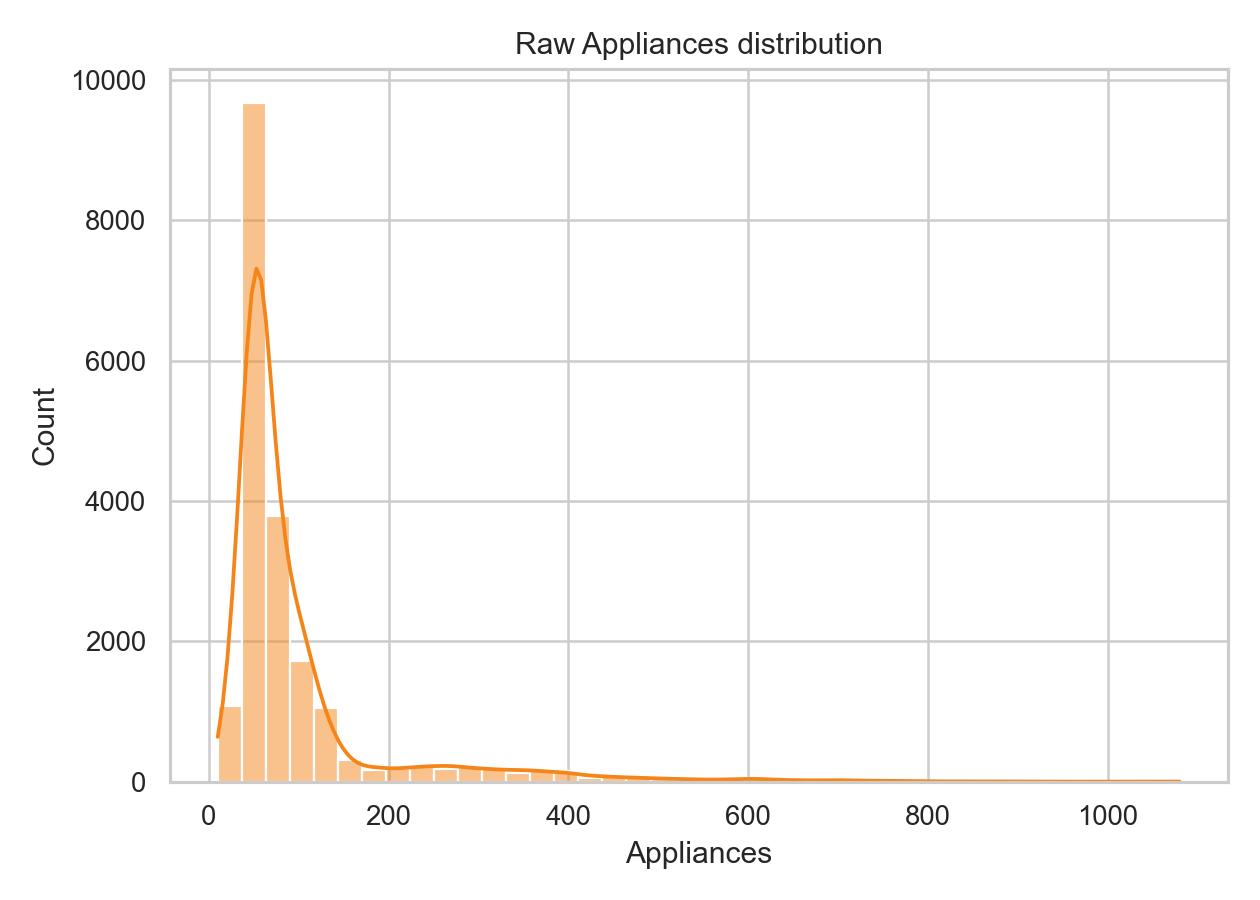
\includegraphics[width=0.78\textwidth]{images/ch1/appliances_energy_distribution_raw.png}
\caption[Minh họa histogram raw Python]{Phân phối gốc (raw) của biến \texttt{Appliances} bằng Python.}
\label{fig:chapter1_histogram_raw}
\end{figure}

\begin{figure}[H]
\centering
\includegraphics[width=0.78\textwidth]{images/ch1/excel_appliances_raw_vs_log_hist_preview.png}
\caption[Minh họa histogram Excel]{Biểu đồ Histogram của biến \texttt{Appliances} được xây dựng trên Excel. Workbook: \texttt{excel/excel\_visualization\_comparison\_native.xlsx}, sheet \texttt{Appliances Histogram}.}
\label{fig:chapter1_histogram_example_excel}
\end{figure}

\textbf{Nhận xét và lý do chọn.} Histogram được chọn vì \texttt{Appliances} là biến định lượng liên tục và câu hỏi đặt ra là ``giá trị tiêu thụ điện phân bố thế nào?''. Hình~\ref{fig:chapter1_histogram_raw} cho thấy phân phối gốc \textbf{lệch phải mạnh}: phần lớn các khung giờ tiêu thụ ít điện (cột cao ở bên trái), trong khi một số ít khung giờ tiêu thụ rất nhiều (đuôi dài kéo sang phải). So sánh Python (Hình~\ref{fig:chapter1_histogram_raw}) và Excel (Hình~\ref{fig:chapter1_histogram_example_excel}) cho thấy hai công cụ cho ra cùng hình dạng lệch phải, tức là kết luận không phụ thuộc công cụ: dữ liệu này không nên đưa thẳng vào mô hình hồi quy mà cần biến đổi log hoặc xử lý dữ liệu bất thường trước. Python phù hợp khi cần tự động hóa và tái lập; Excel phù hợp khi cần kiểm tra nhanh bằng bảng tính.

\subsubsection{Boxplot (Biểu đồ hộp): phát hiện dữ liệu bất thường dựa trên IQR}

Boxplot hiển thị median, $Q_1$, $Q_3$, IQR và các điểm ngoài ngưỡng $Q_1-1.5\times IQR$ hoặc $Q_3+1.5\times IQR$. Đây là biểu đồ quan trọng để phát hiện dữ liệu bất thường và so sánh phân phối giữa các lớp. Ví dụ boxplot cholesterol theo \texttt{target\_binary} cho phép so sánh mức cholesterol giữa nhóm có và không có bệnh tim. Tác dụng phân tích là phát hiện biến cần xử lý ngoại lệ, đồng thời đánh giá biến định lượng có khả năng phân biệt nhãn hay không. \textbf{Hạn chế:} boxplot không mô tả rõ hình dạng phân phối bên trong; dữ liệu đa đỉnh có thể bị che khuất. Điểm ngoài râu hộp chỉ là ứng viên dữ liệu bất thường, cần kiểm tra thêm bằng kiến thức miền.

\begin{table}[H]
\centering
\caption{Dữ liệu mẫu cho boxplot cholesterol theo nhóm bệnh tim}
\label{tab:chapter1_boxplot_sample_data}
\small
\begin{tabular}{rrrr}
\toprule
Mẫu & \texttt{target\_binary} & \texttt{chol} & Ghi chú \\
\midrule
1 & 0 & 233 & Nhóm không bệnh \\
2 & 0 & 250 & Nhóm không bệnh \\
3 & 1 & 204 & Nhóm có bệnh \\
4 & 1 & 236 & Nhóm có bệnh \\
5 & 0 & 354 & Giá trị cao \\
6 & 1 & 564 & Ứng viên dữ liệu bất thường \\
\bottomrule
\end{tabular}
\end{table}

Bảng \ref{tab:chapter1_boxplot_sample_data} cho thấy dữ liệu boxplot cần một biến định lượng và một biến nhóm. Trước khi vẽ, cần tính các đại lượng hộp: $Q_1$, median, $Q_3$, IQR và biên dữ liệu bất thường.

\begin{table}[H]
\centering
\caption{Tính toán trước khi vẽ boxplot cholesterol}
\label{tab:chapter1_boxplot_calc}
\small
\begin{tabular}{lrr}
\toprule
Thành phần boxplot & Công thức/cách lấy & Kết quả \\
\midrule
$Q_1$ & $P_{25}$ của \texttt{chol} & 211 \\
Median & $P_{50}$ của \texttt{chol} & 241 \\
$Q_3$ & $P_{75}$ của \texttt{chol} & 275 \\
IQR & $Q_3-Q_1$ & 64 \\
Biên dưới & $Q_1-1.5\times IQR$ & 115 \\
Biên trên & $Q_3+1.5\times IQR$ & 371 \\
Ứng viên dữ liệu bất thường & \texttt{chol} $>371$ hoặc $<115$ & 564 \\
\bottomrule
\end{tabular}
\end{table}

Từ các kết quả trên có thể vẽ tay boxplot: hộp kéo từ 211 đến 275, đường giữa ở 241, râu dưới kéo dài đến giá trị nhỏ nhất nằm trong khoảng $1.5 \times IQR$ là 126 (mặc dù biên dưới tính toán lý thuyết là 115 nhưng không có dữ liệu thực tế nào nhỏ hơn 126), râu trên kéo dài đến giá trị lớn nhất nằm trong khoảng $1.5 \times IQR$ là 371, và điểm dữ liệu 564 nằm ngoài râu được biểu diễn riêng biệt là dữ liệu bất thường.

\textbf{Ghi chú về Box plot trong workbook Excel.} Box-and-Whisker là kiểu biểu đồ có trong Excel hiện đại, nhưng workbook minh chứng của báo cáo chỉ lưu các chart object native được script dựng tự động và không nhúng ảnh preview. Vì vậy ví dụ boxplot ở phần này được trình bày bằng Python; sheet \texttt{Heart Boxplot} trong workbook chỉ giữ bảng tóm tắt để người đọc có thể tự dựng lại nếu cần.

\begin{figure}[H]
\centering
\includegraphics[width=0.90\textwidth]{images/ch1/heart_disease_cholesterol_boxplot.png}
\caption[Minh họa boxplot Heart Disease]{Minh họa boxplot: cholesterol theo nhóm bệnh tim.}
\label{fig:chapter1_boxplot_example}
\end{figure}

\textbf{Nhận xét và lý do chọn.} Boxplot được chọn vì \texttt{chol} là biến định lượng liên tục và câu hỏi phân tích là ``có dữ liệu bất thường hay không, phân phối hai nhóm target khác nhau thế nào?''. Hình \ref{fig:chapter1_boxplot_example} cho thấy cholesterol có các điểm nằm ngoài vùng râu hộp, tức là có ứng viên dữ liệu bất thường theo quy tắc IQR. Median và IQR giúp đọc cấu trúc trung tâm tốt hơn mean khi dữ liệu có giá trị cực trị. So với histogram, boxplot không mô tả chi tiết hình dạng phân phối, nhưng tốt hơn trong việc so sánh hai nhóm và phát hiện điểm bất thường. Vì vậy, mẫu Heart Disease phù hợp với boxplot khi mục tiêu là đánh giá dữ liệu bất thường và khả năng phân biệt nhóm bệnh/không bệnh.

\textbf{Đánh giá.} Kết quả biểu diễn phân phối biến cholesterol theo \texttt{target\_binary} cho thấy sự khác biệt về trung vị và các điểm dữ liệu bất thường. Python phù hợp cho phiên bản báo cáo vì kiểm soát được định dạng, nhãn và tái lập bằng script.

\subsection{Nhóm biểu đồ tương quan và cơ cấu}

Nhóm biểu đồ tương quan và cơ cấu trả lời hai câu hỏi: ``các biến có liên hệ với nhau không?'' và ``các nhóm định tính chiếm tỷ trọng thế nào?''. Scatter plot và heatmap dùng cho biến định lượng; bar chart và pie chart dùng cho biến định tính. Có thể bổ sung pair plot, hexbin plot, stacked bar chart và mosaic plot khi cần phân tích sâu hơn.

\begin{table}[H]
\centering
\caption{Nhóm biểu đồ tương quan và cơ cấu: ý nghĩa, hạn chế và trường hợp áp dụng}
\label{tab:chapter1_relation_structure_chart_group}
\small
\begin{tabular}{p{0.18\textwidth}p{0.25\textwidth}p{0.25\textwidth}p{0.20\textwidth}}
\toprule
Biểu đồ & Ý nghĩa & Trường hợp áp dụng & Hạn chế \\
\midrule
Biểu đồ phân tán (Scatter plot) & Tìm liên hệ tuyến tính/phi tuyến, cụm, điểm bất thường & \texttt{age}--\texttt{thalach}, nhiệt độ--năng lượng & Dễ xảy ra hiện tượng chồng lấp điểm (overplotting) khi kích thước dữ liệu lớn; chỉ phản ánh mối tương quan trực quan bề mặt mà không thể xác lập quan hệ nhân quả trực tiếp. \\
Biểu đồ cột/tròn (Bar/Pie chart) & Xem cơ cấu định tính, lớp phổ biến/hiếm & \texttt{cp}, \texttt{dx}, \texttt{Diagnosis} & Pie khó so sánh nhiều nhóm; bar không thể hiện quan hệ nếu không nhóm/chồng \\
Bản đồ nhiệt tương quan (Correlation heatmap) & Xem tương quan nhiều biến định lượng & Chọn đặc trưng Heart Disease, Breast Cancer & Chủ yếu phản ánh mối liên hệ tương quan tuyến tính đơn biến (Pearson); không thể hiện được các mối quan hệ phi tuyến phức tạp và không khẳng định quan hệ nhân quả. \\
Biểu đồ cặp/tổ ong (Pair/Hexbin plot) & Xem nhiều cặp biến hoặc mật độ điểm dày & EDA nhiều biến định lượng & Dễ rối, tốn không gian báo cáo \\
Biểu đồ cột chồng/mảnh ghép (Stacked bar/Mosaic) & Xem quan hệ hai biến định tính & \texttt{dx} theo \texttt{localization}, target theo giới tính & Khó đọc khi nhiều nhóm nhỏ \\
\bottomrule
\end{tabular}
\end{table}

\subsubsection{Scatter plot (Biểu đồ phân tán): tìm liên hệ tuyến tính/phi tuyến}

Scatter plot biểu diễn mối quan hệ giữa hai biến định lượng. Nếu các điểm tạo thành xu hướng tăng/giảm, có thể tồn tại liên hệ tuyến tính hoặc phi tuyến. Trong Heart Disease, scatter plot giữa \texttt{age} và \texttt{thalach} giúp kiểm tra xu hướng tuổi cao đi kèm nhịp tim tối đa thấp hơn hay không. Tác dụng phân tích là phát hiện quan hệ biến, cụm quan sát và điểm bất thường theo cặp biến. \textbf{Hạn chế:} khi số điểm quá lớn, điểm bị chồng lên nhau làm khó đọc; xu hướng quan sát được không khẳng định quan hệ nhân quả.

\begin{table}[H]
\centering
\caption{Dữ liệu mẫu cho scatter plot tuổi và nhịp tim tối đa}
\label{tab:chapter1_scatter_sample_data}
\small
\begin{tabular}{rrrr}
\toprule
Mẫu & \texttt{age} & \texttt{thalach} & \texttt{target\_binary} \\
\midrule
1 & 63 & 150 & 0 \\
2 & 67 & 108 & 1 \\
3 & 37 & 187 & 0 \\
4 & 41 & 172 & 0 \\
5 & 56 & 178 & 1 \\
6 & 62 & 160 & 1 \\
\bottomrule
\end{tabular}
\end{table}

Bảng \ref{tab:chapter1_scatter_sample_data} minh họa mỗi dòng là một điểm trên scatter plot. Trước khi vẽ, cần chuyển mỗi dòng thành tọa độ $(x,y)$, với $x=\texttt{age}$ và $y=\texttt{thalach}$; nếu tô màu thì dùng thêm \texttt{target\_binary}.

\begin{table}[H]
\centering
\caption{Tính tọa độ trước khi vẽ scatter plot}
\label{tab:chapter1_scatter_calc}
\small
\begin{tabular}{rrrr}
\toprule
Mẫu & Tọa độ $(x,y)$ & Nhóm màu & Diễn giải \\
\midrule
1 & $(63,150)$ & 0 & Tuổi 63, nhịp tim tối đa 150 \\
2 & $(67,108)$ & 1 & Tuổi 67, nhịp tim tối đa 108 \\
3 & $(37,187)$ & 0 & Tuổi 37, nhịp tim tối đa 187 \\
4 & $(41,172)$ & 0 & Tuổi 41, nhịp tim tối đa 172 \\
5 & $(56,178)$ & 1 & Tuổi 56, nhịp tim tối đa 178 \\
6 & $(62,160)$ & 1 & Tuổi 62, nhịp tim tối đa 160 \\
\bottomrule
\end{tabular}
\end{table}

Từ bảng tọa độ này có thể vẽ tay scatter plot bằng cách đặt từng điểm lên hệ trục; nhóm màu 0/1 giúp phân biệt bệnh/không bệnh.

\textbf{Các bước thao tác vẽ scatter plot bằng Excel.} Để bảo đảm tính tái lập, báo cáo trình bày thao tác cụ thể trên Microsoft Excel cho biểu đồ đại diện ở Bảng \ref{tab:chapter1_scatter_calc} (scatter plot giữa \texttt{age} và \texttt{thalach}, tô màu theo \texttt{target\_binary}):
\begin{enumerate}[leftmargin=2.2em,label=\textbf{Bước \arabic*.}]
 \item \textbf{Chuẩn bị dữ liệu:} mở file \texttt{outputs/cleaned/heart\_disease\_cleaned.csv} trong Excel; đảm bảo ba cột \texttt{age}, \texttt{thalach}, \texttt{target\_binary} nằm cạnh nhau và có hàng tiêu đề (ví dụ để \texttt{age} ở cột A, \texttt{thalach} ở cột B, \texttt{target\_binary} ở cột C).
 \item \textbf{Bôi đen vùng dữ liệu:} quét chọn vùng chứa hai cột \texttt{age} (trục $x$) và \texttt{thalach} (trục $y$), bao gồm cả hàng tiêu đề, ví dụ \texttt{A1:B304}.
 \item \textbf{Chèn biểu đồ:} vào tab \textbf{Insert} $\rightarrow$ nhóm \textbf{Charts} $\rightarrow$ chọn \textbf{Scatter} (biểu tượng điểm chấm) $\rightarrow$ chọn \textbf{Scatter with only Markers}. Excel tự động vẽ các điểm lên hệ trục.
 \item \textbf{Tô màu theo nhóm:} vì một scatter plot mặc định chỉ có một màu, để phân biệt bệnh/không bệnh cần tách dữ liệu thành hai chuỗi (series): chèn thêm cột \texttt{thalach\_0} và \texttt{thalach\_1} dùng hàm \texttt{=IF(C2=0,B2,NA())} và \texttt{=IF(C2=1,B2,NA())}; sau đó chọn \textbf{Select Data} trên biểu đồ $\rightarrow$ \textbf{Add} từng chuỗi với $x$ là cột \texttt{age}, $y$ lần lượt là \texttt{thalach\_0} và \texttt{thalach\_1}; đặt màu khác nhau cho hai chuỗi (ví dụ xanh cho \texttt{target\_binary}=0, đỏ cho \texttt{target\_binary}=1).
 \item \textbf{Định dạng trục và nhãn:} nhấp vào biểu đồ $\rightarrow$ tab \textbf{Chart Design} $\rightarrow$ \textbf{Add Chart Element} $\rightarrow$ đặt \textbf{Axis Titles} là ``Tuổi (age)'' cho trục $x$ và ``Nhịp tim tối đa (thalach)'' cho trục $y$; thêm \textbf{Chart Title} và \textbf{Legend} để ghi rõ ý nghĩa hai màu.
 \item \textbf{(Tuỳ chọn) Đường xu hướng:} để thấy quan hệ âm, nhấp chuột phải vào một chuỗi $\rightarrow$ \textbf{Add Trendline} $\rightarrow$ chọn \textbf{Linear} và tick \textbf{Display Equation on chart}; hệ số góc âm sẽ xác nhận xu hướng ``tuổi tăng, nhịp tim tối đa giảm''.
 \item \textbf{Xuất ảnh:} nhấp chuột phải vào vùng biểu đồ $\rightarrow$ \textbf{Save as Picture} $\rightarrow$ chọn định dạng PNG để đưa vào báo cáo.
\end{enumerate}
Quy trình bảy bước trên áp dụng chung cho mọi scatter plot trong báo cáo; với các biến khác (ví dụ \texttt{T1}--\texttt{Appliances} trong Appliances Energy) chỉ cần thay vùng dữ liệu ở Bước 2. Kết quả thu được ở Hình \ref{fig:chapter1_scatter_example_excel} cho hình dạng xu hướng tương tự phiên bản Python ở Hình \ref{fig:chapter1_scatter_example}, chứng tỏ thao tác Excel và script Python cho ra cùng một kết luận phân tích.

\begin{figure}[H]
\centering
\includegraphics[width=0.90\textwidth]{images/ch1/heart_disease_age_thalach_scatter.png}
\caption[Minh họa scatter plot Python]{Minh họa scatter plot tuổi và nhịp tim tối đa trong Heart Disease bằng Python.}
\label{fig:chapter1_scatter_example}
\end{figure}

\begin{figure}[H]
\centering
\includegraphics[width=0.90\textwidth]{images/ch1/excel_heart_age_thalach_scatter_preview.png}
\caption[Minh họa scatter plot Excel]{Minh họa scatter plot tuổi và nhịp tim tối đa trong Heart Disease bằng Excel. Workbook: \texttt{excel/excel\_visualization\_comparison\_native.xlsx}, sheet \texttt{Heart Scatter}.}
\label{fig:chapter1_scatter_example_excel}
\end{figure}

\textbf{Nhận xét và lý do chọn.} Scatter plot được chọn vì \texttt{age} và \texttt{thalach} đều là biến định lượng, mục tiêu là kiểm tra quan hệ giữa hai biến thay vì chỉ xem từng biến riêng lẻ. Hình \ref{fig:chapter1_scatter_example} cho thấy xu hướng âm: tuổi tăng thì nhịp tim tối đa có xu hướng giảm. So với histogram và boxplot, scatter plot biểu diễn từng cặp quan sát nên phù hợp để phát hiện quan hệ tuyến tính, phi tuyến, cụm điểm hoặc điểm bất thường theo cặp biến. Python và Excel cho hình dạng xu hướng tương tự; Python thuận tiện khi cần tô màu theo target hoặc tính correlation, còn Excel giúp kiểm tra nhanh bằng thao tác trực quan.

\subsubsection{Bar chart/Pie chart (Biểu đồ cột/tròn): cơ cấu định tính}

Bar chart và pie chart dùng cho biến định tính. Bar chart để so sánh tần suất giữa các nhóm; pie chart để mô tả tỷ trọng khi số nhóm ít và tỷ lệ cần trình bày nhanh. Trong báo cáo, bar chart được ưu tiên hơn pie chart vì dễ so sánh hơn, đặc biệt với các biến có nhiều lớp như \texttt{localization} trong HAM10000. Tác dụng phân tích là nhận diện mất cân bằng lớp, lớp hiếm và cơ cấu dữ liệu đầu vào. \textbf{Hạn chế:} pie chart khó so sánh khi có nhiều nhóm hoặc tỷ lệ gần nhau; bar chart chỉ mô tả cơ cấu một biến nếu không mở rộng thành grouped/stacked bar.

\begin{table}[H]
\centering
\caption{Dữ liệu mẫu cho bar chart loại đau ngực}
\label{tab:chapter1_bar_sample_data}
\small
\begin{tabular}{lrr}
\toprule
Loại đau ngực \texttt{cp} & Tần suất & Tỷ lệ xấp xỉ \\
\midrule
1 & 23 & 7.6\% \\
2 & 50 & 16.5\% \\
3 & 86 & 28.4\% \\
4 & 144 & 47.5\% \\
\bottomrule
\end{tabular}
\end{table}

Bảng \ref{tab:chapter1_bar_sample_data} là dữ liệu đã tổng hợp theo nhóm. Trước khi vẽ bar chart hoặc pie chart, cần tính tần suất và tỷ lệ: $p_j=f_j/n$ với $n=303$.

\begin{table}[H]
\centering
\caption{Tính toán trước khi vẽ bar chart/pie chart biến \texttt{cp}}
\label{tab:chapter1_bar_calc}
\small
\begin{tabular}{lrrr}
\toprule
Giá trị \texttt{cp} & $f_j$ & $p_j=f_j/303$ & Góc pie chart \\
\midrule
1 & 23 & 7.6\% & 27.3$^\circ$ \\
2 & 50 & 16.5\% & 59.4$^\circ$ \\
3 & 86 & 28.4\% & 102.2$^\circ$ \\
4 & 144 & 47.5\% & 171.1$^\circ$ \\
\bottomrule
\end{tabular}
\end{table}

Từ bảng này có thể vẽ tay bar chart bằng chiều cao cột $f_j$; nếu vẽ pie chart thì dùng góc $p_j\times360^\circ$ cho từng lát cắt.

\begin{figure}[H]
\centering
\includegraphics[width=0.90\textwidth]{images/ch1/heart_disease_chest_pain_bar.png}
\caption[Minh họa bar chart Python]{Minh họa bar chart tần suất loại đau ngực Heart Disease bằng Python.}
\label{fig:chapter1_bar_example}
\end{figure}

\begin{figure}[H]
\centering
\includegraphics[width=0.90\textwidth]{images/ch1/excel_heart_cp_bar_preview.png}
\caption[Minh họa bar chart Excel]{Minh họa bar chart tần suất loại đau ngực Heart Disease bằng Excel. Workbook: \texttt{excel/excel\_visualization\_comparison\_native.xlsx}, sheet \texttt{Heart Frequency}.}
\label{fig:chapter1_bar_example_excel}
\end{figure}

\textbf{Nhận xét và lý do chọn.} Bar chart được chọn vì \texttt{cp} là biến định tính/rời rạc, biểu diễn loại đau ngực. Với biến loại nhóm, histogram không phù hợp vì các mã 1--4 không phải thang đo liên tục; scatter plot cũng không có ý nghĩa nếu chỉ phân tích một biến định tính. Hình \ref{fig:chapter1_bar_example} cho thấy \texttt{cp=4} chiếm nhiều nhất, tức cơ cấu loại đau ngực không cân bằng. Bar chart tốt hơn pie chart trong mẫu này vì người đọc dễ so sánh chiều cao cột giữa bốn nhóm. Python và Excel cho cùng thứ tự nhóm, chứng minh bảng tần suất được tính nhất quán giữa hai công cụ.

\textbf{Trực quan hóa dữ liệu bằng biểu đồ tròn (Pie Chart): So sánh dạng 2D và 3D.} Trong trực quan hóa dữ liệu khoa học, biểu đồ tròn dạng 2D được coi là chuẩn mực trình bày, trong khi biểu đồ tròn 3D ít được khuyến nghị sử dụng. Bản chất góc nghiêng phối cảnh và chiều sâu của không gian 3D làm sai lệch tỷ lệ thị giác của người xem: các phân phần nằm ở phía trước (gần mắt nhìn hơn) trông sẽ lớn hơn thực tế, ngược lại các phần ở phía sau bị thu nhỏ lại dù có cùng tỷ trọng. Điều này dễ dẫn đến việc ước lượng sai lệch cấu trúc dữ liệu.

Hơn nữa, việc sử dụng hiệu ứng tách mảnh (exploded pie chart) trong không gian 3D càng làm gia tăng độ méo hình học, do chiều cao của miếng bánh tạo ra thể tích ảo không tỷ lệ thuận với giá trị thực tế của dữ liệu. Biểu đồ tròn 2D duy trì chính xác tỷ lệ góc ở tâm $\theta_i = p_i \times 360^\circ$ (như tính toán ở bảng thống kê cơ cấu lớp), giúp truyền tải cấu trúc thuộc tính định tính một cách trung thực nhất. Do đó, toàn bộ biểu đồ cột và biểu đồ tròn trong nghiên cứu này đều được thống nhất biểu diễn dưới dạng 2D phẳng để đảm bảo tính khách quan và chuẩn mực khoa học.

\subsection{Các dạng biểu đồ khác}

Nhóm này dùng cho các trường hợp ngoài phân phối một biến, tương quan hai biến hoặc cơ cấu định tính đơn giản. Các dạng quan trọng gồm line chart cho chuỗi thời gian, rolling mean/area chart để làm mượt hoặc nhấn mạnh xu hướng, confusion matrix để đánh giá phân loại, prediction vs actual để đánh giá hồi quy/dự báo, image grid để kiểm tra dữ liệu ảnh.

\begin{table}[H]
\centering
\caption{Các dạng biểu đồ khác: ý nghĩa, hạn chế và trường hợp áp dụng}
\label{tab:chapter1_other_chart_group}
\small
\begin{tabular}{p{0.18\textwidth}p{0.25\textwidth}p{0.25\textwidth}p{0.20\textwidth}}
\toprule
Biểu đồ & Ý nghĩa & Trường hợp áp dụng & Hạn chế \\
\midrule
Line chart & Trend, seasonality, biến động theo thời gian & Appliances Energy, HAR, MHEALTH & Dễ nhiễu nếu dữ liệu dao động mạnh \\
Rolling mean/Area chart & Làm mượt hoặc nhấn mạnh tổng lượng & Tiêu thụ điện theo ngày/tuần & Che mất biến động ngắn hạn \\
Confusion matrix & Lỗi phân loại theo lớp & Heart Disease, HAM10000, Breast Cancer & Cần mô hình đã huấn luyện; phụ thuộc ngưỡng \\
Prediction vs Actual & So sánh dự báo và thực tế & Regression/dự báo Appliances & Không chỉ rõ nguyên nhân sai số \\
Image grid/montage & Kiểm tra chất lượng ảnh, lỗi nhãn & HAM10000 & Chủ quan, chỉ xem được mẫu nhỏ \\
\bottomrule
\end{tabular}
\end{table}

\subsubsection{Line chart (Biểu đồ đường) cho chuỗi thời gian}

Line chart đặt thời gian trên trục hoành và giá trị quan sát trên trục tung. Biểu đồ này bắt buộc với nhóm B để phân tích trend, seasonality, biến động bất thường và thời điểm thay đổi. Với Appliances Energy, dữ liệu có 19,735 mẫu từ 2016-01-11 17:00:00 đến 2016-05-27 18:00:00, tần suất phổ biến 10 phút/mẫu. Do đó line chart theo ngày được dùng để làm mượt xu hướng tiêu thụ năng lượng. Tác dụng phân tích là chọn cách chia train/test theo thời gian và đánh giá biến động trước khi dự báo. \textbf{Hạn chế:} line chart dễ bị nhiễu nếu tần suất lấy mẫu dày và biến động mạnh; cần sắp xếp thời gian đúng, xử lý missing timestamp và cân nhắc rolling mean.

\begin{table}[H]
\centering
\caption{Dữ liệu mẫu cho line chart Appliances Energy theo thời gian}
\label{tab:chapter1_line_sample_data}
\small
\begin{tabular}{lr}
\toprule
Thời điểm & \texttt{Appliances} \\
\midrule
2016-01-11 17:00 & 60 \\
2016-01-11 17:10 & 60 \\
2016-01-11 17:20 & 50 \\
2016-01-11 17:30 & 50 \\
2016-01-11 17:40 & 60 \\
2016-01-11 17:50 & 50 \\
\bottomrule
\end{tabular}
\end{table}

Bảng \ref{tab:chapter1_line_sample_data} cho thấy điều kiện cần của line chart là có biến thời gian được sắp xếp. Trước khi vẽ, cần chuyển từng dòng thành điểm $(t,y)$, với $t$ là thời điểm và $y=\texttt{Appliances}$; nếu vẽ đường trung bình trượt thì tính thêm rolling mean.

\begin{table}[H]
\centering
\caption{Tính tọa độ và rolling mean trước khi vẽ line chart}
\label{tab:chapter1_line_calc}
\small
\begin{tabular}{lrr}
\toprule
Thời điểm & $y_t$ & Rolling mean 3 mẫu \\
\midrule
2016-01-11 17:00 & 60 & -- \\
2016-01-11 17:10 & 60 & -- \\
2016-01-11 17:20 & 50 & 56.67 \\
2016-01-11 17:30 & 50 & 53.33 \\
2016-01-11 17:40 & 60 & 53.33 \\
2016-01-11 17:50 & 50 & 53.33 \\
\bottomrule
\end{tabular}
\end{table}

Công thức rolling mean 3 mẫu là $\bar{y}_{t,3}=(y_t+y_{t-1}+y_{t-2})/3$, ví dụ tại 17:20: $(60+60+50)/3=56.67$. Từ bảng này có thể vẽ tay line chart bằng cách nối các điểm theo thứ tự thời gian.

\begin{figure}[H]
\centering
\includegraphics[width=0.90\textwidth]{images/ch1/appliances_energy_daily_line.png}
\caption[Minh họa line chart Python]{Minh họa line chart tiêu thụ năng lượng theo ngày trong Appliances Energy bằng Python.}
\label{fig:chapter1_line_example}
\end{figure}

\begin{figure}[H]
\centering
\includegraphics[width=0.90\textwidth]{images/ch1/excel_appliances_daily_line_preview.png}
\caption[Minh họa line chart Excel]{Minh họa line chart tiêu thụ năng lượng theo ngày trong Appliances Energy bằng Excel. Workbook: \texttt{excel/excel\_visualization\_comparison\_native.xlsx}, sheet \texttt{Appliances Daily}.}
\label{fig:chapter1_line_example_excel}
\end{figure}

\textbf{Nhận xét và lý do chọn.} Line chart được chọn vì Appliances Energy có trục thời gian rõ ràng, mỗi quan sát gắn với thời điểm thu thập. Nếu dùng histogram, ta chỉ biết phân phối mức tiêu thụ nhưng mất thông tin thứ tự thời gian; nếu dùng bar chart, xu hướng theo ngày không rõ. Hình \ref{fig:chapter1_line_example} cho thấy mức tiêu thụ dao động theo ngày, có các giai đoạn tăng/giảm và các điểm cao bất thường. So sánh Python và Excel cho thấy xu hướng tổng thể thống nhất. Vì vậy, line chart là lựa chọn phù hợp nhất để phân tích trend, seasonality và làm cơ sở cho quyết định chia train/test theo thời gian ở bài toán dự báo.

\subsubsection{Correlation heatmap (Bản đồ nhiệt tương quan): tương quan nhiều biến định lượng}

Correlation heatmap biểu diễn ma trận tương quan giữa các biến định lượng. Màu sắc giúp nhận diện nhanh cặp biến có tương quan dương hoặc âm. Biểu đồ này hữu ích trong bước lựa chọn đặc trưng và phát hiện đa cộng tuyến trước khi huấn luyện mô hình.

Hệ số tương quan Pearson giữa hai biến $X$ và $Y$ được tính bằng:

\begin{equation}
r_{XY} = \frac{\sum_{i=1}^{n}(x_i-\bar{x})(y_i-\bar{y})}{\sqrt{\sum_{i=1}^{n}(x_i-\bar{x})^2}\sqrt{\sum_{i=1}^{n}(y_i-\bar{y})^2}}
\end{equation}

Giá trị $r_{XY}$ nằm trong khoảng $[-1, 1]$. Giá trị gần 1 biểu thị tương quan dương mạnh; gần -1 biểu thị tương quan âm mạnh; gần 0 biểu thị mối quan hệ tuyến tính yếu. Tuy nhiên, tương quan không đồng nghĩa với quan hệ nhân quả, nên heatmap chỉ nên được xem là công cụ thăm dò ban đầu.

\begin{table}[H]
\centering
\caption{Dữ liệu mẫu cho correlation heatmap Heart Disease}
\label{tab:chapter1_heatmap_sample_data}
\small
\begin{tabular}{rrrrr}
\toprule
Mẫu & \texttt{age} & \texttt{trestbps} & \texttt{chol} & \texttt{thalach} \\
\midrule
1 & 63 & 145 & 233 & 150 \\
2 & 67 & 160 & 286 & 108 \\
3 & 37 & 130 & 250 & 187 \\
4 & 41 & 130 & 204 & 172 \\
5 & 56 & 120 & 236 & 178 \\
6 & 62 & 140 & 268 & 160 \\
\bottomrule
\end{tabular}
\end{table}

Bảng \ref{tab:chapter1_heatmap_sample_data} gồm nhiều biến định lượng trên cùng các mẫu. Từ bảng này, hệ số tương quan được tính cho từng cặp biến, sau đó đưa vào ma trận màu của heatmap. Để chứng minh heatmap không phải hình vẽ ngẫu nhiên, Bảng \ref{tab:chapter1_heatmap_calc} đưa ra một số hệ số tương quan đã tính trước khi tô màu.

\begin{table}[H]
\centering
\caption{Tính toán tương quan trước khi vẽ heatmap}
\label{tab:chapter1_heatmap_calc}
\small
\begin{tabular}{lrr}
\toprule
Cặp biến & Hệ số $r$ & Ý nghĩa màu \\
\midrule
\texttt{age} -- \texttt{thalach} & -0.39 & Tương quan âm, màu lạnh \\
\texttt{age} -- \texttt{trestbps} & 0.28 & Tương quan dương yếu, màu ấm nhạt \\
\texttt{chol} -- \texttt{trestbps} & 0.13 & Gần trung tính \\
\texttt{chol} -- \texttt{thalach} & -0.01 & Gần 0, màu trung tính \\
\bottomrule
\end{tabular}
\end{table}

Từ các hệ số này có thể vẽ tay heatmap bằng cách lập ma trận biến--biến, ghi $r$ vào từng ô và gán màu theo độ lớn/dấu của $r$.

\begin{figure}[H]
\centering
\includegraphics[width=0.95\textwidth]{images/ch1/heart_disease_correlation_heatmap.png}
\caption[Minh họa correlation heatmap Heart Disease]{Minh họa correlation heatmap: tương quan biến trong Heart Disease.}
\label{fig:chapter1_heatmap_example}
\end{figure}

\textbf{Nhận xét và lý do chọn.} Correlation heatmap được chọn vì Heart Disease có nhiều biến định lượng và cần xem nhanh quan hệ giữa nhiều cặp biến cùng lúc. Nếu chỉ dùng scatter plot, mỗi hình chỉ thể hiện một cặp biến; heatmap gom toàn bộ ma trận tương quan vào một hình, giúp phát hiện cặp biến có liên hệ dương/âm mạnh và các nhóm biến có khả năng trùng thông tin. Hình \ref{fig:chapter1_heatmap_example} phù hợp cho bước chọn đặc trưng trước khi học máy. Tuy nhiên, heatmap chỉ phản ánh tương quan tuyến tính, không chứng minh quan hệ nhân quả và không thay thế kiểm định thống kê hay kiến thức chuyên ngành y tế.

\textbf{Ghi chú về Excel.} Excel không có chart object heatmap riêng; workbook chỉ lưu ma trận tương quan ở sheet \texttt{Heart Corr} với conditional formatting, không nhúng ảnh preview. Vì vậy hình minh họa heatmap trong báo cáo được tính là biểu đồ Python.

\subsection{Một số dạng biểu đồ bổ sung phù hợp với bài toán}

Ngoài sáu dạng chính, báo cáo đề xuất thêm ba biểu đồ mới có khả năng bổ sung trực tiếp cho phân tích trong các chương sau: raincloud plot cho phân phối theo lớp, ridgeline plot cho nhiều phân phối song song và hexbin plot cho dữ liệu hai biến có mật độ điểm cao. Ba biểu đồ này không thay thế histogram, boxplot hoặc scatter plot; chúng được dùng khi biểu đồ cơ bản bắt đầu che mất mật độ, chồng điểm hoặc khác biệt nhỏ giữa nhiều nhóm. Các biểu đồ mới được khai báo trong Bảng \ref{tab:chapter1_extra_chart_types} trước khi minh họa chi tiết.

\begin{table}[H]
\centering
\caption{Đề xuất 3 biểu đồ mới: ưu điểm, nhược điểm và phạm vi áp dụng}
\label{tab:chapter1_extra_chart_types}
\small
\begin{tabular}{p{0.16\textwidth}p{0.25\textwidth}p{0.21\textwidth}p{0.21\textwidth}p{0.12\textwidth}}
\toprule
Biểu đồ mới & Giới thiệu & Ưu điểm & Nhược điểm & Phạm vi áp dụng \\
\midrule
Raincloud plot & Kết hợp density/violin, boxplot và điểm dữ liệu thô trong cùng một hình. & Vừa thấy hình dạng phân phối, median/IQR, vừa thấy từng quan sát; tốt hơn boxplot khi cần giải thích sự chồng lấn giữa các lớp. & Dễ rối nếu số lớp nhiều hoặc mẫu quá lớn; cần chú thích rõ để người đọc không quen vẫn hiểu. & So sánh biến định lượng theo lớp: \texttt{chol} theo \texttt{target\_binary}, độ sáng ảnh HAM10000 theo \texttt{dx}. \\
Ridgeline plot & Xếp nhiều density plot theo hàng ngang để so sánh nhiều nhóm hoặc nhiều mốc thời gian. & Tiết kiệm không gian khi có nhiều phân phối; dễ nhận ra dịch chuyển trung tâm, độ lệch và đa đỉnh giữa các nhóm. & Không phù hợp nếu nhóm quá ít; phần chồng lớp có thể gây hiểu nhầm diện tích nếu thang đo không thống nhất. & So sánh phân phối \texttt{Appliances} theo tháng/ngày trong tuần hoặc phân phối tuổi theo lớp bệnh. \\
Hexbin plot & Chia mặt phẳng hai biến thành các ô lục giác và tô màu theo số điểm trong mỗi ô. & Giải quyết overplotting tốt hơn scatter plot khi dữ liệu nhiều điểm; màu thể hiện mật độ quan sát. & Mất thông tin từng điểm; kết quả phụ thuộc kích thước ô và thang màu. & Cặp biến định lượng dày điểm: \texttt{T1}--\texttt{Appliances}, \texttt{age}--\texttt{thalach}, đặc trưng ảnh số hóa. \\
\bottomrule
\end{tabular}
\end{table}

\subsubsection{Raincloud plot (Biểu đồ mưa-mây) cho phân phối theo lớp}

Raincloud plot trong Bảng \ref{tab:chapter1_extra_chart_types} kết hợp ba lớp thông tin: density/violin để thấy hình dạng phân phối, boxplot để đọc median và IQR, và điểm jitter để thấy quan sát thô. Biểu đồ này phù hợp khi cần so sánh biến định lượng giữa các nhóm nhưng boxplot đơn lẻ chưa cho biết mật độ điểm tập trung ở đâu. Với Heart Disease, raincloud plot có thể dùng cho \texttt{chol} theo \texttt{target\_binary}. Dữ liệu đầu vào gồm hai cột: nhãn bệnh \texttt{target\_binary} và cholesterol \texttt{chol}; mỗi nhóm được vẽ một nửa density, một hộp IQR và các điểm jitter. Nếu nhóm có bệnh có đuôi phải dài hơn, biểu đồ cho thấy khác biệt không chỉ ở median mà còn ở mật độ và dữ liệu bất thường. \textbf{Hạn chế:} raincloud plot dễ rối khi có quá nhiều lớp hoặc quá nhiều điểm; cần chú thích rõ ý nghĩa của density, hộp IQR và điểm dữ liệu.

\subsubsection{Ridgeline plot (Biểu đồ sống núi) cho nhiều phân phối song song}

Ridgeline plot trong Bảng \ref{tab:chapter1_extra_chart_types} xếp nhiều đường mật độ theo từng nhóm hoặc từng mốc thời gian. Biểu đồ này phù hợp khi cần so sánh nhiều phân phối cùng lúc mà histogram hoặc KDE riêng lẻ chiếm quá nhiều không gian. Với Appliances Energy, ridgeline plot được dùng để so sánh phân phối \texttt{log1p(Appliances)} theo tháng. Dữ liệu đầu vào gồm tháng trích từ biến thời gian và giá trị \texttt{Appliances\_log1p}; mỗi tháng tạo một density riêng, xếp chồng theo trục dọc. Nếu một tháng có density lệch phải hơn tháng khác, người phân tích có cơ sở kiểm tra yếu tố mùa vụ hoặc thay đổi hành vi tiêu thụ. \textbf{Hạn chế:} ridgeline plot có thể gây hiểu nhầm nếu thang mật độ không thống nhất hoặc các đường chồng quá mạnh; nên dùng cùng thang đo và sắp xếp nhóm theo thời gian.

\begin{figure}[H]
\centering
\includegraphics[width=0.92\textwidth]{images/ch1/appliances_energy_monthly_ridgeline.png}
\caption[Minh họa ridgeline Appliances Energy]{Minh họa ridgeline plot: phân phối \texttt{log1p(Appliances)} theo từng tháng.}
\label{fig:chapter1_ridgeline_example_inline}
\end{figure}

\textbf{Ghi chú về Excel.} Excel không có chart ridgeline native, nên báo cáo không xem ridgeline là biểu đồ Excel. Sheet \texttt{Appliances Ridgeline} chỉ lưu dữ liệu \texttt{month + log1p} để người đọc có thể dựng nhiều histogram theo tháng nếu cần; hình ridgeline trong báo cáo được render bằng Python.

\subsubsection{Hexbin plot (Biểu đồ tổ ong) cho dữ liệu hai biến dày điểm}

Hexbin plot trong Bảng \ref{tab:chapter1_extra_chart_types} chia mặt phẳng hai biến thành các ô lục giác và tô màu theo số quan sát trong từng ô. Biểu đồ này phù hợp khi scatter plot bị overplotting, tức nhiều điểm chồng lên nhau làm người đọc không thấy vùng mật độ cao. Với dữ liệu 19,735 mẫu của Appliances Energy, hexbin plot giữa \texttt{T1} và \texttt{Appliances} phù hợp hơn scatter plot vì mỗi ô màu đậm cho biết vùng nhiệt độ phòng và mức tiêu thụ điện xuất hiện thường xuyên. Với Heart Disease, hexbin cũng có thể dùng cho cặp \texttt{age}--\texttt{thalach} nếu mở rộng sang dữ liệu lớn hơn. \textbf{Hạn chế:} hexbin plot làm mất thông tin từng điểm riêng lẻ; kết quả phụ thuộc kích thước ô và thang màu, nên cần chọn tham số nhất quán khi so sánh nhiều hình.

\begin{table}[H]
\centering
\caption{Dữ liệu mẫu minh họa ba biểu đồ mới}
\label{tab:chapter1_extra_chart_sample_data}
\small
\begin{tabular}{lrrrr}
\toprule
Dataset & Biến nhóm/thời gian & Biến $x$ & Biến $y$ & Biểu đồ phù hợp \\
\midrule
Heart Disease & \texttt{target\_binary} & -- & \texttt{chol} & Raincloud plot \\
Heart Disease & \texttt{target\_binary} & -- & \texttt{thalach} & Raincloud plot \\
Appliances Energy & Tháng/ngày trong tuần & -- & \texttt{Appliances} & Ridgeline plot \\
Appliances Energy & -- & \texttt{T1} & \texttt{Appliances} & Hexbin plot \\
HAM10000 & \texttt{dx} & -- & Mean intensity & Raincloud/Ridgeline plot \\
\bottomrule
\end{tabular}
\end{table}

\begin{figure}[H]
\centering
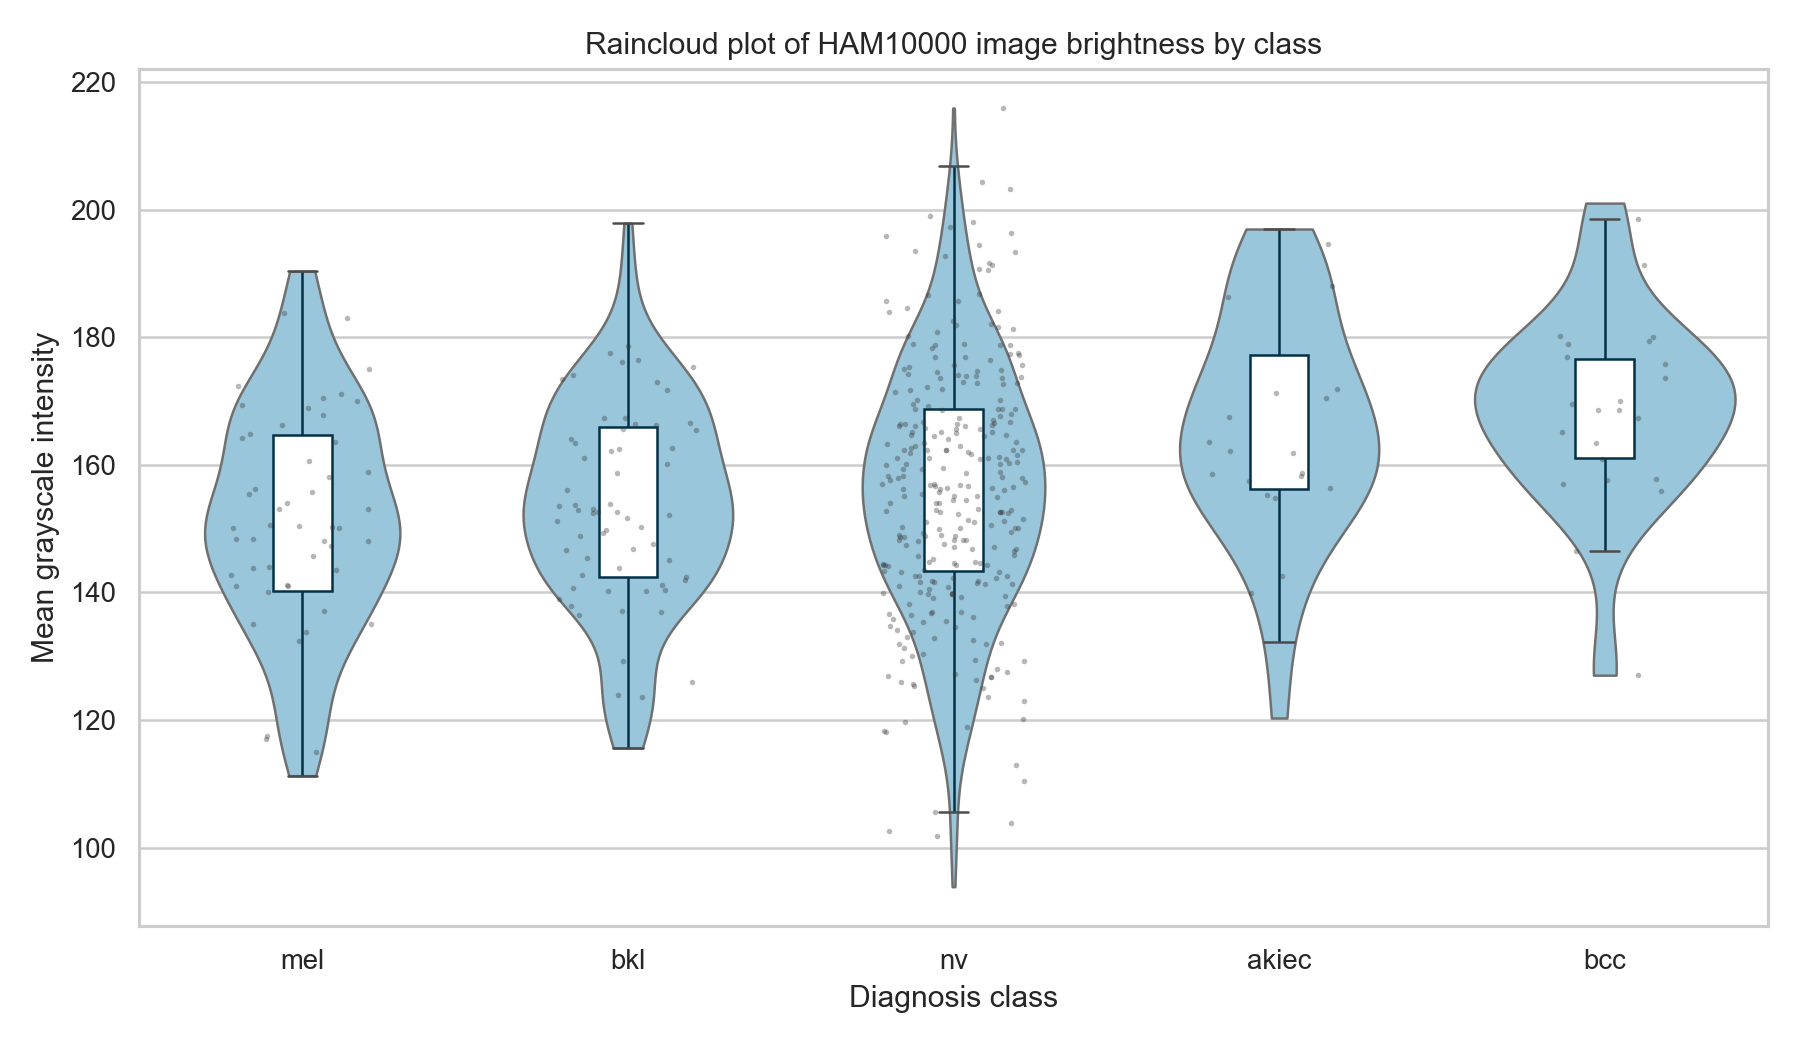
\includegraphics[width=0.90\textwidth]{images/ch1/ham10000_mean_intensity_raincloud.png}
\caption[Minh họa raincloud plot HAM10000]{Biểu đồ mưa-mây (Raincloud plot) thể hiện đồng thời phân phối mật độ nhân (KDE), biểu đồ hộp và phân phối điểm của độ sáng ảnh theo lớp.}
\label{fig:chapter1_extra_chart_examples}
\end{figure}

\begin{figure}[H]
\centering
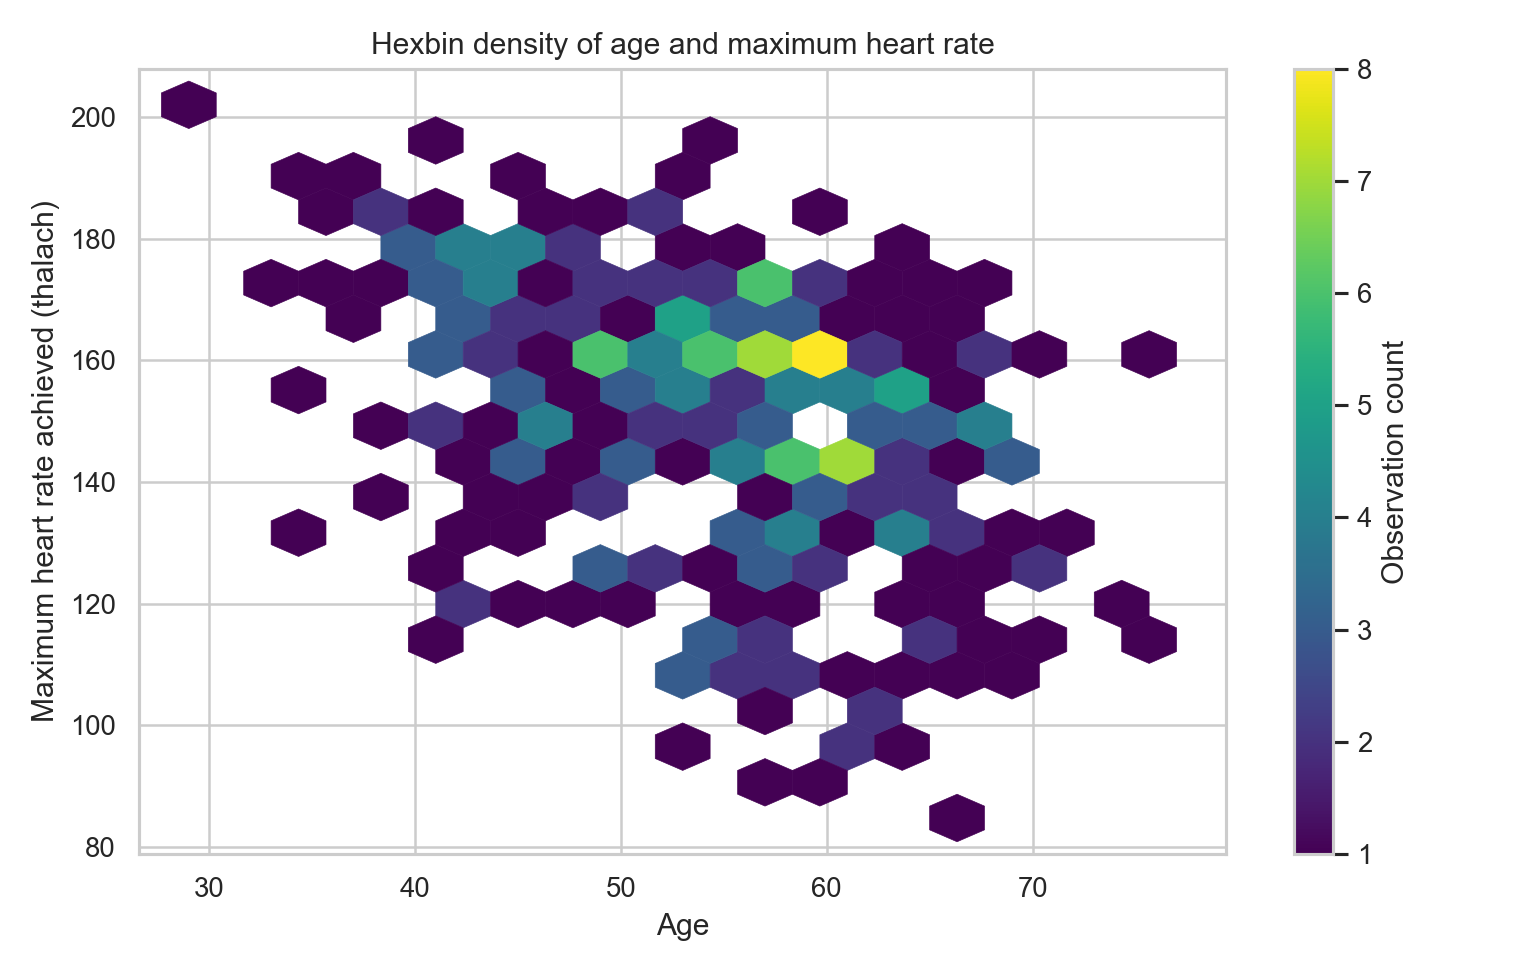
\includegraphics[width=0.90\textwidth]{images/ch1/heart_age_thalach_hexbin.png}
\caption[Minh họa hexbin plot Heart Disease]{Biểu đồ tổ ong (Hexbin plot) thể hiện mật độ phân bố đồng thời của thuộc tính Tuổi và Nhịp tim tối đa, giúp khắc phục hiện tượng chồng lấp điểm dữ liệu.}
\label{fig:chapter1_extra_chart_examples_hexbin}
\end{figure}

\textbf{Nhận xét và lý do chọn.} Ba biểu đồ mới được chọn vì mỗi biểu đồ xử lý một hạn chế cụ thể của biểu đồ cơ bản. Raincloud plot mở rộng boxplot khi cần thấy cả density và điểm dữ liệu; ridgeline plot mở rộng KDE khi cần so sánh nhiều nhóm/thời đoạn; hexbin plot mở rộng scatter plot khi điểm quan sát quá dày. Trong báo cáo, chúng nên được dùng có chọn lọc: chỉ thêm khi câu hỏi phân tích cần mật độ phân phối, nhiều nhóm song song hoặc dữ liệu hai biến quá đông điểm. Nếu mục tiêu chỉ là mô tả đơn giản, histogram, boxplot và scatter plot vẫn là lựa chọn dễ đọc hơn.

\section{Các phép biến đổi và tiền xử lý cơ bản}

Các phép biến đổi và tiền xử lý là cầu nối giữa thống kê mô tả và mô hình hóa. Theo Han, Kamber và Pei, chất lượng dữ liệu ảnh hưởng trực tiếp đến chất lượng khai phá dữ liệu; dữ liệu thiếu, nhiễu, lệch thang đo hoặc không dừng có thể làm mô hình học sai cấu trúc thật \cite{Han2011DataMining}. Trong học máy ứng dụng, Kuhn và Johnson cũng nhấn mạnh rằng tiền xử lý và feature engineering phải được quyết định dựa trên bản chất biến, phân phối và thuật toán sử dụng, không nên áp dụng máy móc cho mọi cột \cite{Kuhn2019FeatureEngineering}. Với dữ liệu chuỗi thời gian, Hyndman và Athanasopoulos khuyến nghị xử lý biến đổi phương sai, sai phân và kiểm tra thứ tự thời gian trước khi dự báo \cite{Hyndman2021Forecasting}.

\subsection{Điền khuyết}

Dữ liệu thực tế thường có missing value do lỗi nhập liệu, lỗi cảm biến, file bị ghép thiếu hoặc một số thuộc tính không đo được ở mọi mẫu. Nếu bỏ toàn bộ dòng thiếu, kích thước mẫu có thể giảm mạnh và tạo thiên lệch nếu missing không ngẫu nhiên. Vì vậy, cần chọn cách điền khuyết theo kiểu biến và nguyên nhân thiếu. Với biến định lượng cân bằng, mean giữ nguyên trung bình tổng thể; với biến định lượng lệch hoặc có dữ liệu bất thường, median bền vững hơn; với biến định tính, mode giữ lại lớp phổ biến nhất.

\begin{equation}
x_{missing} =
\begin{cases}
median(X), & \text{nếu X là biến định lượng có dữ liệu bất thường} \\
mean(X), & \text{nếu X là biến định lượng cân bằng} \\
mode(X), & \text{nếu X là biến định tính}
\end{cases}
\end{equation}

\textbf{Trường hợp/phạm vi áp dụng.} Điền mean/median phù hợp khi tỷ lệ thiếu thấp và biến thiếu không phải nhãn mục tiêu. Điền mode phù hợp với biến phân loại có số lớp ít. Với chuỗi thời gian, nên ưu tiên nội suy, forward fill hoặc backward fill nếu giá trị liền kề có ý nghĩa thời gian. Không nên điền khuyết tùy tiện khi tỷ lệ thiếu quá cao, khi missing mang ý nghĩa riêng, hoặc khi biến thiếu là target cần dự báo.

\textbf{Ví dụ cụ thể.} Trong Heart Disease, biến \texttt{ca} thiếu 4 giá trị và \texttt{thal} thiếu 2 giá trị. Vì tỷ lệ thiếu thấp, có thể điền \texttt{ca} bằng median/mode sau khi xem phân phối, và điền \texttt{thal} bằng mode vì đây là biến phân loại được mã hóa. Trong Appliances Energy, các biến cảm biến nếu có khoảng trống ngắn nên dùng nội suy tuyến tính theo thời gian để giữ xu hướng liên tục thay vì điền mean toàn cục.

\subsection{Chuẩn hóa thang đo}

Trong học máy, các biến có thang đo khác nhau có thể làm thuật toán dựa trên khoảng cách hoặc gradient bị lệch. Ví dụ, cholesterol có miền khoảng hàng trăm, còn \texttt{oldpeak} chỉ khoảng 0--6; nếu dùng K-Means hoặc SVM mà không chuẩn hóa, biến có đơn vị lớn dễ chi phối khoảng cách. Hai kỹ thuật cơ bản là min-max scaling và standardization.

Min-max scaling đưa giá trị về khoảng $[0,1]$:

\begin{equation}
x' = \frac{x - x_{min}}{x_{max} - x_{min}}
\end{equation}

Standardization đưa dữ liệu về mean 0 và standard deviation 1:

\begin{equation}
x' = \frac{x - \mu}{\sigma}
\end{equation}

\textbf{Trường hợp/phạm vi áp dụng.} Min-max scaling phù hợp khi cần giữ miền cố định, ví dụ đặc trưng ảnh đưa về $[0,1]$ hoặc mô hình neural network. Standardization phù hợp hơn cho Logistic Regression, SVM, PCA, K-Means và Hierarchical Clustering vì các thuật toán này nhạy với thang đo. Không bắt buộc chuẩn hóa cho cây quyết định và Random Forest vì chúng tách theo ngưỡng từng biến, nhưng chuẩn hóa vẫn có thể hữu ích khi so sánh hệ số hoặc kết hợp với thuật toán khác.

\textbf{Ví dụ cụ thể.} Với Heart Disease, trước khi chạy K-Means, các biến \texttt{age}, \texttt{trestbps}, \texttt{chol}, \texttt{thalach}, \texttt{oldpeak} cần standardization để \texttt{chol} không áp đảo khoảng cách. Với HAM10000, nếu trích đặc trưng độ sáng trung bình từ ảnh, giá trị pixel nên chia cho 255 để đưa về $[0,1]$ trước khi so sánh giữa ảnh.

\subsection{Log transform và differencing cho chuỗi thời gian}
\label{sec:logtransform}

Log transform dùng khi biến định lượng lệch phải mạnh, có nhiều giá trị nhỏ nhưng một số giá trị rất lớn. Phép biến đổi này nén phần đuôi phải, giảm ảnh hưởng của giá trị cực trị và giúp mô hình tuyến tính dễ học hơn. Với dữ liệu chuỗi thời gian, log transform còn giúp phương sai ổn định hơn trước khi dự báo \cite{Hyndman2021Forecasting}:

\begin{equation}
y'_t = \log(1 + y_t)
\end{equation}

Sai phân bậc 1 giúp loại bỏ xu hướng cục bộ và chuyển phân tích từ mức giá trị sang mức thay đổi:

\begin{equation}
\Delta y_t = y_t - y_{t-1}
\end{equation}

\textbf{Trường hợp/phạm vi áp dụng.} Log1p phù hợp với biến không âm và lệch phải như \texttt{Appliances}, chi phí, doanh thu, số lượt truy cập hoặc cường độ pixel tổng hợp. Không dùng log trực tiếp cho giá trị âm; khi có 0 nên dùng \texttt{log1p}. Differencing phù hợp cho chuỗi thời gian có xu hướng hoặc mức nền thay đổi; tuy nhiên nếu sai phân quá mức có thể làm mất thông tin dài hạn và tăng nhiễu.

\textbf{Ví dụ cụ thể.} Trong Appliances Energy, \texttt{Appliances\_log1p} và \texttt{Appliances\_diff} đã được tạo trong script \texttt{src/analyze\_appliances\_energy.py}. Histogram raw cho thấy \texttt{Appliances} lệch phải, còn histogram log1p gọn hơn. Line chart theo ngày và ridgeline plot theo tháng giúp kiểm tra liệu phân phối tiêu thụ điện có thay đổi theo thời gian hay không. Khi xây dựng mô hình dự báo, dữ liệu phải chia train/test theo thứ tự thời gian, không random split, để tránh rò rỉ thông tin tương lai.

\begin{table}[H]
\centering
\caption{Tóm tắt phạm vi áp dụng các phép tiền xử lý cơ bản}
\label{tab:chapter1_preprocess_scope}
\small
\begin{tabular}{p{0.18\textwidth}p{0.27\textwidth}p{0.25\textwidth}p{0.20\textwidth}}
\toprule
Kỹ thuật & Áp dụng khi & Không nên dùng khi & Ví dụ trong báo cáo \\
\midrule
Mean/median/mode imputation & Tỷ lệ thiếu thấp, biến đầu vào quan trọng & Missing quá cao hoặc missing là tín hiệu riêng & \texttt{ca}, \texttt{thal} trong Heart Disease \\
Nội suy thời gian & Chuỗi thời gian có khoảng trống ngắn & Khoảng trống dài, cảm biến lỗi kéo dài & Cảm biến Appliances Energy \\
Min-max scaling & Cần miền $[0,1]$, dữ liệu ảnh/neural network & Có dữ liệu bất thường mạnh chưa xử lý & Độ sáng ảnh HAM10000 \\
Standardization & SVM, Logistic Regression, PCA, K-Means & Cần giữ đơn vị gốc để giải thích trực tiếp & Các biến Heart Disease trước clustering \\
Log1p transform & Biến không âm lệch phải & Dữ liệu âm hoặc cần diễn giải đơn vị gốc & \texttt{Appliances\_log1p} \\
Differencing & Chuỗi có xu hướng, cần phân tích thay đổi & Chuỗi quá nhiễu hoặc cần mức tuyệt đối & \texttt{Appliances\_diff} \\
\bottomrule
\end{tabular}
\end{table}

\section{Quy trình phân tích khám phá dữ liệu}

Phân tích khám phá dữ liệu (Exploratory Data Analysis - EDA) là giai đoạn nối giữa dữ liệu thô và mô hình phân tích. Nếu bỏ qua EDA, người phân tích có thể đưa vào mô hình các biến bị lỗi kiểu dữ liệu, phân phối lệch quá mạnh, chứa dữ liệu bất thường bất thường hoặc có target mất cân bằng. Trong báo cáo này, EDA được xem như một quy trình có kiểm soát gồm năm bước.

\begin{enumerate}[leftmargin=2.2em,label=\textbf{\arabic*.}]
 \item \textbf{Kiểm tra cấu trúc dữ liệu}: xác định số dòng, số cột, kiểu dữ liệu, khóa thời gian, nhãn mục tiêu và các file nguồn.
 \item \textbf{Kiểm tra chất lượng dữ liệu}: tìm giá trị thiếu, giá trị trùng, giá trị ngoài miền hợp lý và kiểu dữ liệu bị đọc sai.
 \item \textbf{Thống kê mô tả}: tính mean, median, mode, percentile, variance, standard deviation, CV và IQR cho các biến định lượng; lập bảng tần suất cho biến định tính.
 \item \textbf{Trực quan hóa}: chọn biểu đồ phù hợp với bản chất biến và câu hỏi phân tích.
 \item \textbf{Rút kết luận phân tích}: ghi nhận đặc điểm dữ liệu có ảnh hưởng đến tiền xử lý, feature engineering và mô hình học máy.
\end{enumerate}

Điểm quan trọng là EDA không dừng ở việc tạo ra nhiều hình. Mỗi hình phải trả lời một câu hỏi cụ thể. Ví dụ, histogram trả lời câu hỏi ``biến này phân phối như thế nào?'', boxplot trả lời câu hỏi ``biến này có dữ liệu bất thường không?'', scatter plot trả lời câu hỏi ``hai biến có quan hệ gì không?'', còn line chart trả lời câu hỏi ``dữ liệu thay đổi ra sao theo thời gian?''.

\begin{table}[H]
\centering
\caption{Quy trình EDA và sản phẩm đầu ra cần lưu}
\label{tab:chapter1_eda_outputs}
\small
\begin{tabular}{p{0.20\textwidth}p{0.32\textwidth}p{0.34\textwidth}}
\toprule
Bước & Câu hỏi chính & Sản phẩm đầu ra \\
\midrule
Kiểm kê dữ liệu & Dữ liệu có bao nhiêu dòng/cột? & Inventory CSV, mô tả dataset \\
Kiểm tra thiếu & Biến nào thiếu và thiếu bao nhiêu? & Missing-value table \\
Thống kê mô tả & Trung tâm và độ phân tán ra sao? & Summary table \\
Trực quan hóa & Phân phối, dữ liệu bất thường, quan hệ biến thế nào? & PNG figure, Excel chart \\
Diễn giải & Kết quả tác động gì đến mô hình? & Nhận xét trong báo cáo \\
\bottomrule
\end{tabular}
\end{table}

Bảng \ref{tab:chapter1_eda_outputs} cũng là cơ sở tổ chức thư mục của dự án. Các file trong \texttt{outputs/tables/} lưu bằng chứng dạng bảng; các file trong \texttt{outputs/figures/} lưu biểu đồ; các file trong \texttt{src/} lưu script tạo kết quả. Cách tổ chức này giúp báo cáo không chỉ có kết luận, mà còn có đường dẫn tái lập kết luận.

\section{Nguyên tắc chọn biểu đồ theo câu hỏi phân tích}

Không có một loại biểu đồ nào phù hợp cho mọi dữ liệu. Việc chọn biểu đồ phụ thuộc vào loại biến, số biến cần so sánh và câu hỏi đang đặt ra. Nếu chọn sai biểu đồ, người đọc có thể hiểu sai bản chất dữ liệu. Ví dụ, dùng pie chart cho biến có quá nhiều lớp sẽ khó so sánh; dùng scatter plot cho biến định tính sẽ không có ý nghĩa; dùng line chart cho dữ liệu không có thứ tự thời gian có thể tạo cảm giác có xu hướng giả.

\begin{table}[H]
\centering
\caption{Chọn biểu đồ theo loại câu hỏi phân tích}
\label{tab:chapter1_chart_by_question}
\small
\begin{tabular}{p{0.24\textwidth}p{0.26\textwidth}p{0.34\textwidth}}
\toprule
Câu hỏi phân tích & Biểu đồ ưu tiên & Lý do sử dụng \\
\midrule
Biến định lượng phân phối thế nào? & Histogram & Nhìn được dạng lệch, nhiều đỉnh, tập trung \\
Có dữ liệu bất thường không? & Boxplot & Dựa trên median, IQR và điểm ngoài ngưỡng \\
Hai biến số có quan hệ không? & Scatter plot & Thể hiện từng cặp quan sát trên mặt phẳng \\
Biến định tính có cơ cấu ra sao? & Bar chart & So sánh tần suất giữa các lớp rõ hơn pie chart \\
Dữ liệu thay đổi theo thời gian thế nào? & Line chart & Giữ thứ tự thời gian và phát hiện xu hướng \\
Nhiều biến liên hệ với nhau ra sao? & Correlation heatmap & Tóm tắt ma trận tương quan bằng màu sắc \\
\bottomrule
\end{tabular}
\end{table}

Trong báo cáo này, nguyên tắc chọn biểu đồ được áp dụng nhất quán. Với Heart Disease, histogram và boxplot được dùng để minh họa phân phối và dữ liệu bất thường; scatter plot và heatmap được dùng để khảo sát quan hệ biến. Với Appliances Energy, line chart là bắt buộc vì dữ liệu có trục thời gian. Với HAM10000, bar chart được dùng cho phân phối lớp, còn boxplot được dùng cho đặc trưng độ sáng sau khi số hóa ảnh.

\section{Diễn giải thống kê trong bối cảnh dữ liệu}

Một chỉ số thống kê chỉ có ý nghĩa khi được đọc trong bối cảnh dữ liệu. Mean không chỉ là một con số trung bình; nó cho biết mức đại diện nếu phân phối tương đối cân bằng. Median không chỉ là vị trí giữa; nó giúp so sánh với mean để nhận biết độ lệch. Standard deviation không chỉ đo độ phân tán; nó còn cho biết biến nào có dao động lớn và có thể cần chuẩn hóa. IQR không chỉ phục vụ boxplot; nó là nền tảng của quy tắc phát hiện dữ liệu bất thường.

Khi đọc một biến định lượng, báo cáo sử dụng ba lớp nhận xét:

\begin{itemize}[leftmargin=1.6em,label=\textbullet]
 \item \textbf{Nhận xét trung tâm}: mean và median gần hay xa nhau, biến có nghiêng lệch hay không.
 \item \textbf{Nhận xét phân tán}: standard deviation, range, IQR lớn hay nhỏ so với mean.
 \item \textbf{Nhận xét tiền xử lý}: có cần cắt dữ liệu bất thường, log-transform, chuẩn hóa hay không.
\end{itemize}

Ví dụ, trong Appliances Energy, mean của \texttt{Appliances} lớn hơn median và max rất cao, cho thấy target lệch phải. Nhận xét này dẫn trực tiếp đến việc dùng \texttt{log1p}. Ngược lại, trong Heart Disease, median của \texttt{chol} gần như không đổi trước và sau tiền xử lý, trong khi max giảm mạnh; điều này cho thấy tiền xử lý chủ yếu làm giảm ảnh hưởng của điểm cực trị, không làm thay đổi phần lõi của phân phối.

\section{Các sai lệch thường gặp khi đọc biểu đồ}

Trực quan hóa giúp dữ liệu dễ hiểu hơn, nhưng cũng có thể gây hiểu nhầm nếu không đọc đúng. Một số sai lệch thường gặp trong báo cáo dữ liệu gồm:

\begin{itemize}[leftmargin=1.6em,label=\textbullet]
 \item \textbf{Nhầm tương quan với nhân quả}: heatmap chỉ cho biết hai biến thay đổi cùng nhau, không chứng minh biến này gây ra biến kia.
 \item \textbf{Đánh giá mô hình chỉ bằng accuracy}: nếu target mất cân bằng, accuracy cao có thể chỉ do mô hình dự đoán lớp đa số.
 \item \textbf{Bỏ qua scale}: các biến có thang đo khác nhau làm scatter plot và thuật toán khoảng cách khó diễn giải nếu chưa chuẩn hóa.
 \item \textbf{Dùng biểu đồ tổng thể thay cho phân tích theo lớp}: phân phối toàn bộ dữ liệu có thể che mất khác biệt giữa các nhóm target.
 \item \textbf{Không gắn biểu đồ với câu hỏi}: một hình đẹp nhưng không trả lời câu hỏi phân tích thì không giúp cải thiện báo cáo.
\end{itemize}

Do đó, mỗi biểu đồ trong báo cáo được viết kèm lý do chọn biểu đồ và nhận xét. Cách trình bày này giúp người đọc hiểu không chỉ biểu đồ thể hiện gì, mà còn vì sao nó cần thiết cho bài toán phân tích dữ liệu.

\section{Minh họa tính toán trên Heart Disease}

Bộ Heart Disease Cleveland có 303 mẫu và 14 thuộc tính gốc được dùng phổ biến trong các thực nghiệm. Trong quá trình đọc dữ liệu, ký hiệu \texttt{?} được chuyển thành missing value. Bảng missing cho thấy biến \texttt{ca} thiếu 4 giá trị, tương đương 1.3201\%, và biến \texttt{thal} thiếu 2 giá trị, tương đương 0.6601\%.

\begin{table}[H]
\centering
\caption{Ví dụ thống kê mô tả trên một số biến Heart Disease}
\label{tab:chapter1_heart_stats}
\begin{tabular}{lrrrrr}
\toprule
Biến & Mean & Median & Std & Min & Max \\
\midrule
age & 54.44 & 56.00 & 9.04 & 29.00 & 77.00 \\
trestbps & 131.69 & 130.00 & 17.60 & 94.00 & 200.00 \\
chol & 246.69 & 241.00 & 51.78 & 126.00 & 564.00 \\
thalach & 149.61 & 153.00 & 22.88 & 71.00 & 202.00 \\
oldpeak & 1.04 & 0.80 & 1.16 & 0.00 & 6.20 \\
\bottomrule
\end{tabular}
\end{table}

Từ Bảng \ref{tab:chapter1_heart_stats}, có thể rút ra ba nhận xét ban đầu. Thứ nhất, biến \texttt{age} có median 56 và mean 54.44, cho thấy phân phối tuổi hơi nghiêng về nhóm trung niên và cao tuổi. Thứ hai, \texttt{chol} có range rất lớn, từ 126 đến 564, nên cần kiểm tra dữ liệu bất thường bằng boxplot. Thứ ba, \texttt{oldpeak} có median 0.8 nhưng mode 0.0, cho thấy một phần đáng kể bệnh nhân không có ST depression.

\begin{table}[H]
\centering
\caption{So sánh trước và sau tiền xử lý trên Heart Disease}
\label{tab:chapter1_preprocess_compare}
\small
\begin{tabular}{lrrrr}
\toprule
Biến & Mean thô & Mean sạch & Std thô & Std sạch \\
\midrule
trestbps & 131.69 & 131.35 & 17.60 & 16.65 \\
chol & 246.69 & 245.58 & 51.78 & 47.56 \\
thalach & 149.61 & 149.65 & 22.88 & 22.73 \\
oldpeak & 1.04 & 1.02 & 1.16 & 1.11 \\
ca & 0.67 & 0.63 & 0.94 & 0.86 \\
\bottomrule
\end{tabular}
\end{table}

Bảng \ref{tab:chapter1_preprocess_compare} cho thấy tiền xử lý không làm thay đổi mạnh giá trị trung tâm, nhưng làm giảm độ biến động của các biến có dữ liệu bất thường. Trường hợp rõ nhất là \texttt{chol}: standard deviation giảm từ 51.78 xuống 47.56, max giảm từ 564 xuống 371. Điều này phù hợp với mục tiêu của tiền xử lý: giữ lại cấu trúc chính của dữ liệu nhưng hạn chế ảnh hưởng của điểm cực trị.

\begin{figure}[H]
\centering
\includegraphics[width=0.90\textwidth]{images/ch1/heart_disease_age_raw_vs_cleaned.png}
\caption[Ví dụ histogram tuổi trên Heart Disease]{Ví dụ histogram tuổi trước/sau xử lý trên Heart Disease.}
\label{fig:chapter1_hist_box}
\end{figure}

\begin{figure}[H]
\centering
\includegraphics[width=0.90\textwidth]{images/ch1/heart_disease_cholesterol_boxplot.png}
\caption[Ví dụ boxplot cholesterol trên Heart Disease]{Ví dụ boxplot cholesterol theo nhãn bệnh trên Heart Disease.}
\label{fig:heart_chol_boxplot}
\end{figure}

\textbf{Lý do chọn biểu đồ.} Histogram được dùng vì biến \texttt{age} là biến định lượng, cần quan sát hình dạng phân phối trước và sau xử lý. Boxplot được dùng vì \texttt{chol} dễ có dữ liệu bất thường và cần so sánh theo nhãn bệnh.

\textbf{Nhận xét.} Hình \ref{fig:chapter1_hist_box} minh họa hai cách đọc dữ liệu khác nhau. Histogram tuổi cho thấy mẫu Heart Disease tập trung ở nhóm trung niên và cao tuổi. Boxplot cholesterol theo nhãn bệnh giúp kiểm tra phân phối cholesterol của nhóm có bệnh và không có bệnh có khác nhau rõ ràng hay không. Nếu hai hộp IQR chồng lắp nhiều, riêng cholesterol có thể không đủ mạnh để phân loại mà cần kết hợp với các biến khác.

\begin{figure}[H]
\centering
\includegraphics[width=0.90\textwidth]{images/ch1/heart_disease_age_thalach_scatter.png}
\caption[Ví dụ scatter plot trên Heart Disease]{Ví dụ scatter plot age và thalach trên Heart Disease.}
\label{fig:chapter1_scatter_heatmap}
\end{figure}

\begin{figure}[H]
\centering
\includegraphics[width=0.95\textwidth]{images/ch1/heart_disease_correlation_heatmap.png}
\caption[Ví dụ correlation heatmap trên Heart Disease]{Ví dụ correlation heatmap trên Heart Disease.}
\label{fig:heart_corr_heatmap}
\end{figure}

\textbf{Lý do chọn biểu đồ.} Scatter plot phù hợp để kiểm tra quan hệ giữa hai biến định lượng \texttt{age} và \texttt{thalach}; heatmap phù hợp để xem nhanh toàn bộ ma trận tương quan.

\textbf{Nhận xét.} Hình \ref{fig:chapter1_scatter_heatmap} minh họa vai trò của trực quan hóa đa biến. Scatter plot cho phép quan sát mối quan hệ giữa tuổi và nhịp tim tối đa, đồng thời tô màu theo nhãn bệnh. Heatmap cho phép nhìn nhanh cặp biến nào có liên hệ tuyến tính mạnh. Trong quy trình phân tích, hai biểu đồ này giúp hình thành giả thuyết trước khi đưa dữ liệu vào mô hình học máy.

\section{Liên kết lý thuyết với các chương sau}

Chương 2 cung cấp ngôn ngữ chung để đọc các kết quả ở Chương 4 và Chương 5. Các chỉ số mean, median, IQR và standard deviation sẽ được dùng để so sánh trước/sau tiền xử lý. Các biểu đồ histogram, boxplot, line chart và heatmap sẽ được dùng để phát hiện đặc trưng dữ liệu. Các nhận xét này tiếp tục làm cơ sở cho lựa chọn mô hình, diễn giải sai số và so sánh với nghiên cứu liên quan.


\chapter{THU THẬP, MÔ TẢ VÀ TỔNG QUAN CÁC BỘ DỮ LIỆU}

\startcontents[chapters]
\printmyminitoc{
Chương này trình bày nguồn gốc, cấu trúc, đặc điểm và mục đích sử dụng của các bộ dữ liệu trong báo cáo. Theo yêu cầu bài tập, nhóm dữ liệu được chia thành ba nhóm: dữ liệu dạng bảng, dữ liệu chuỗi thời gian/cảm biến và dữ liệu đa phương tiện.
}

\section{Tiêu chí lựa chọn dữ liệu}

Tiêu chí lựa chọn dữ liệu được xây dựng theo yêu cầu của đề bài và khả năng phân tích thực tế trong báo cáo. Mỗi bộ dữ liệu được đưa vào phải thuộc đúng một trong ba nhóm A, B hoặc C; có số mẫu và số biến đạt ngưỡng tối thiểu; có nguồn gốc rõ ràng; đồng thời có thể phục vụ các nội dung thống kê mô tả, trực quan hóa, tiền xử lý và học máy ở các chương sau.

Đối với nhóm A, dữ liệu phải là dạng bảng, có ít nhất hơn 5 thuộc tính và hơn 100 quan sát để phù hợp với phân tích biến định tính, biến định lượng và bài toán phân loại. Đối với nhóm B, dữ liệu phải có bản chất chuỗi thời gian hoặc tín hiệu/cảm biến, có hơn 500 quan sát để có thể biểu diễn xu hướng và đánh giá mô hình dự báo hoặc phân loại theo thời gian. Đối với nhóm C, dữ liệu phải thuộc nhóm đa phương tiện như ảnh hoặc văn bản, đủ lớn để trích xuất đặc trưng số và phân tích phân phối lớp.

Ngoài các tiêu chí định lượng, báo cáo ưu tiên những bộ dữ liệu có tài liệu mô tả, biến mục tiêu rõ ràng, đã được sử dụng trong nghiên cứu hoặc benchmark, và có khả năng tái lập bằng mã nguồn Python trong thư mục dự án. Nhờ vậy, việc lựa chọn dữ liệu không chỉ nhằm đáp ứng số lượng mà còn bảo đảm tính nhất quán giữa Chương 2, Chương 3 và Chương 4.

\section{Chiến lược thu thập và kiểm chứng dữ liệu}

Việc chọn dữ liệu trong báo cáo không chỉ nhằm đủ số lượng bộ dữ liệu theo đề bài, mà còn phải bảo đảm mỗi bộ dữ liệu có thể tạo ra phân tích thống kê, trực quan hóa và thí nghiệm học máy có ý nghĩa. Do đó, nhóm áp dụng bốn tiêu chí khi quyết định đưa một dataset vào báo cáo.

\begin{enumerate}
    \item \textbf{Tính phù hợp với nhóm dữ liệu}: dataset phải thuộc một trong ba nhóm A, B, C theo mô tả bài toán.
    \item \textbf{Khả năng phân tích thống kê}: dataset cần có biến định lượng hoặc biến định tính đủ rõ để tính thống kê, lập bảng tần suất và vẽ biểu đồ.
    \item \textbf{Khả năng học máy}: dataset nên có target hoặc có cấu trúc đặc trưng đủ tốt để phục vụ classification, regression hoặc clustering.
    \item \textbf{Khả năng tái lập}: dữ liệu, script, bảng kết quả, biểu đồ và log phải được lưu lại trong thư mục dự án.
\end{enumerate}

Với tiêu chí này, các bộ dữ liệu được chọn không đứng độc lập mà tạo thành một pipeline xuyên suốt. Heart Disease được dùng để minh họa lý thuyết, phân tích thống kê và classification. Appliances Energy được dùng để minh họa chuỗi thời gian và regression. HAM10000 và Reuters-21578 đại diện cho dữ liệu đa phương tiện, nơi dữ liệu thô cần được số hóa thành đặc trưng trước khi thống kê.

\begin{table}[H]
\centering
\caption{Vai trò của từng bộ dữ liệu trong toàn bộ báo cáo}
\label{tab:chapter2_dataset_role_matrix}
\small
\begin{tabular}{p{0.22\textwidth}p{0.18\textwidth}p{0.24\textwidth}p{0.24\textwidth}}
\toprule
Dataset & Nhóm & Vai trò thống kê & Vai trò học máy \\
\midrule
Heart Disease & A & Minh họa lý thuyết, outlier, tần suất & Classification, clustering \\
CDC Diabetes & A & Tần suất biến sức khỏe/hành vi & Classification nguy cơ tiểu đường \\
Breast Cancer & A & Histogram, boxplot, heatmap & Classification khối u \\
Appliances Energy & B & Line chart, phân phối target & Regression/time-series forecasting \\
HAR & B & Phân phối activity, cảm biến & Activity classification, clustering \\
MHEALTH & B & Thống kê tín hiệu cảm biến & Activity classification, clustering \\
HAM10000 & C & Phân phối lớp, đặc trưng ảnh & Image classification, clustering \\
Reuters-21578 & C & Độ dài văn bản, tần suất topic & Text classification \\
\bottomrule
\end{tabular}
\end{table}

Bảng \ref{tab:chapter2_dataset_role_matrix} cho thấy mỗi dataset đều có một vai trò cụ thể, tránh tình trạng thu thập dữ liệu chỉ để đủ số lượng. Đây cũng là căn cứ để Chương 3 và Chương 4 mở rộng phân tích theo từng nhóm.


Yêu cầu bài tập đặt ra ba nhóm dữ liệu chính. Nhóm A là dữ liệu dạng bảng, cần tối thiểu 3 bộ, mỗi bộ có hơn 5 features và hơn 100 samples. Nhóm B là dữ liệu chuỗi thời gian, cần tối thiểu 3 bộ, mỗi bộ có hơn 500 samples. Nhóm C là dữ liệu đa phương tiện, cần ít nhất 2 bộ trong các loại ảnh, audio, video hoặc text.

Trong quá trình thực hiện, báo cáo chọn 8 bộ dữ liệu để bao phủ cả ba nhóm. Các bộ dữ liệu được ưu tiên vì có nguồn công khai, có số mẫu đủ lớn, có bài toán học máy rõ ràng và có khả năng sinh bảng/hình/log minh chứng bằng Python. Bảng \ref{tab:dataset_overview} tóm tắt danh sách dữ liệu đã thu thập.

\begin{table}[H]
\centering
\caption{Đối chiếu bộ dữ liệu với yêu cầu đề bài}
\label{tab:chapter2_requirement_compliance}
\small
\begin{tabular}{p{0.18\textwidth}p{0.18\textwidth}p{0.16\textwidth}p{0.20\textwidth}p{0.18\textwidth}}
\toprule
Nhóm yêu cầu & Dataset sử dụng & Ngưỡng đề bài & Minh chứng đáp ứng & Artifact trong dự án \\
\midrule
A -- tabular & Heart Disease & $>5$ feature, $>100$ mẫu & 13 feature, 303 mẫu & \texttt{datasets/heart+disease/} \\
A -- tabular & CDC Diabetes & $>5$ feature, $>100$ mẫu & 21 feature, 253680 mẫu & \texttt{datasets/uci\_891\_cdc\_diabetes\_health\_indicators/} \\
A -- tabular & Breast Cancer & $>5$ feature, $>100$ mẫu & 30 feature, 569 mẫu & \texttt{datasets/breast+cancer+wisconsin+diagnostic/} \\
B -- chuỗi/cảm biến & Appliances Energy & $>500$ mẫu & 19735 mẫu, có mốc thời gian & \texttt{datasets/appliances+energy+prediction/} \\
B -- chuỗi/cảm biến & HAR & $>500$ mẫu & 10299 mẫu cảm biến & \texttt{datasets/human+activity+recognition/} \\
B -- chuỗi/cảm biến & MHEALTH & $>500$ mẫu & 1215745 mẫu cảm biến & \texttt{datasets/mhealth+dataset/} \\
C -- ảnh & HAM10000 & $\geq 500$ ảnh & 10015 ảnh/metadata & \texttt{datasets/skin-cancer-mnist-ham10000/} \\
C -- văn bản & Reuters-21578 & $\geq 1000$ văn bản & 21578 văn bản & \texttt{datasets/reuters-21578/} \\
\bottomrule
\end{tabular}
\end{table}

Bảng \ref{tab:chapter2_requirement_compliance} cho thấy lựa chọn dữ liệu vượt ngưỡng tối thiểu của đề bài: nhóm A có đủ ba bộ bảng, nhóm B có đủ ba bộ chuỗi/thứ tự quan sát, nhóm C có hai dạng multimedia là ảnh và văn bản. Việc ghi rõ thư mục artifact giúp báo cáo có tính tái lập: người đọc có thể kiểm tra dữ liệu thô, script phân tích trong \texttt{src/}, bảng xuất trong \texttt{outputs/tables/} và hình xuất trong \texttt{outputs/figures/}.

\begin{table}[H]
\centering
\caption{Tổng hợp các bộ dữ liệu sử dụng trong báo cáo}
\label{tab:dataset_overview}
\small
\begin{tabular}{llllr}
\toprule
ID & Nhóm & Bộ dữ liệu & Bài toán chính & Số mẫu \\
\midrule
A1 & A & Heart Disease & Classification & 303 \\
A2 & A & CDC Diabetes Health Indicators & Classification & 253680 \\
A3 & A & Breast Cancer Wisconsin Diagnostic & Classification & 569 \\
B1 & B & Appliances Energy Prediction & Regression & 19735 \\
B2 & B & Human Activity Recognition & Classification & 10299 \\
B3 & B & MHEALTH & Classification & 1215745 \\
C1 & C & HAM10000 & Image classification & 10015 \\
C2 & C & Reuters-21578 & Text classification & 21578 \\
\bottomrule
\end{tabular}
\end{table}


\section{Nhóm A: Dữ liệu dạng bảng}

Nhóm A gồm ba bộ dữ liệu dạng bảng, mỗi dòng là một quan sát độc lập và mỗi cột là một thuộc tính có kiểu dữ liệu rõ ràng. Các bảng mô tả trong phần này tập trung vào: số lượng mẫu, kiểu dữ liệu của feature, ý nghĩa thực tế và kết quả baseline dùng làm mốc đối sánh cho Chương 4.

\begin{table}[H]
\centering
\caption{Tổng hợp yêu cầu mô tả dữ liệu bảng nhóm A}
\label{tab:group_a_rubric_summary}
\small
\begin{tabular}{lllll}
\toprule
Dataset & Số mẫu & Số feature & Target & Bài toán \\
\midrule
A1 Heart Disease & 303 & 13 + target & num & Classification/clustering \\
A2 CDC Diabetes & 253680 & 21 + target & Diabetes\_binary & Classification \\
A3 Breast Cancer & 569 & 30 + target & Diagnosis & Classification \\
\bottomrule
\end{tabular}
\end{table}

\subsection{A1 - Heart Disease}

\textbf{Nguồn gốc và cấu trúc dữ liệu.} Heart Disease là bộ dữ liệu y khoa từ UCI Machine Learning Repository. Thư mục local là \path{datasets/heart+disease/}. Bộ dữ liệu gốc gồm Cleveland, Hungarian, Switzerland và Long Beach VA; trong báo cáo dùng bản Cleveland processed với 303 mẫu và 14 thuộc tính. Biến mục tiêu là \texttt{num}, trong đó 0 biểu diễn không có bệnh tim và 1--4 biểu diễn các mức có bệnh.

\textbf{Trường dữ liệu và phân phối.} Các biến chính gồm thông tin nhân khẩu học, triệu chứng lâm sàng và kết quả xét nghiệm: \texttt{age}, \texttt{sex}, \texttt{cp}, \texttt{trestbps}, \texttt{chol}, \texttt{thalach}, \texttt{oldpeak}, \texttt{ca}, \texttt{thal} và \texttt{num}. Phân phối target gồm 164 mẫu lớp 0 (54.13\%), 55 mẫu lớp 1, 36 mẫu lớp 2, 35 mẫu lớp 3 và 13 mẫu lớp 4; khi quy về nhị phân, hai nhóm không bệnh/có bệnh khá cân bằng. Tuổi bệnh nhân có trung bình 54.44, trung vị 56 và trải từ 29 đến 77. Cholesterol có trung bình 246.69 và giá trị lớn nhất ban đầu 564, sau làm sạch được chặn còn 371 để giảm ảnh hưởng outlier. \texttt{thalach} có trung bình 149.61, phản ánh nhịp tim tối đa khi gắng sức; \texttt{oldpeak} có trung vị 0.8 và giá trị cực đại được giảm từ 6.2 xuống 4.0 sau xử lý. Dữ liệu có missing value ở \texttt{ca} và \texttt{thal}, nên đây là ví dụ phù hợp để minh họa điền khuyết, mã hóa biến phân loại và chuẩn hóa trước khi học máy.

\textbf{Tổng quan bài báo liên quan.} Detrano và cộng sự xây dựng mô hình xác suất hỗ trợ chẩn đoán bệnh mạch vành từ dữ liệu lâm sàng, nhấn mạnh khả năng dùng biến bệnh án thường quy để ước lượng nguy cơ \cite{Detrano1989HeartDisease}. Aha và Kibler dùng cùng nhóm dữ liệu để đánh giá instance-based learning; trọng tâm của bài báo là đo khoảng cách giữa các hồ sơ bệnh nhân và ra quyết định dựa trên các ca tương tự \cite{Aha1991InstanceBased}. Gennari và cộng sự khai thác hướng conceptual clustering/classification qua hệ thống CLASSIT, cho thấy dữ liệu nhỏ nhưng giàu ý nghĩa y khoa vẫn có thể dùng để tạo nhóm khái niệm có thể diễn giải \cite{Gennari1989CLASSIT}. Nhìn chung, các nghiên cứu đạt được kết quả quan trọng ở mức phương pháp: chứng minh Heart Disease là benchmark phù hợp cho mô hình tuyến tính, k-NN, cây quyết định và ensemble; đồng thời cho thấy tính diễn giải của đặc trưng lâm sàng là yếu tố quan trọng hơn mô hình quá phức tạp.

\begin{table}[H]
\centering
\caption{Các biến chính trong Heart Disease}
\label{tab:heart_feature_dictionary}
\small
\begin{tabular}{llll}
\toprule
Biến & Loại & Ý nghĩa & Vai trò \\
\midrule
age & Định lượng rời rạc & Tuổi bệnh nhân & Feature \\
sex & Định tính & Giới tính & Feature \\
cp & Định tính & Loại đau ngực & Feature \\
trestbps & Liên tục & Huyết áp nghỉ ngơi & Feature \\
chol & Liên tục & Cholesterol huyết thanh & Feature \\
thalach & Liên tục & Nhịp tim tối đa & Feature \\
oldpeak & Liên tục & ST depression & Feature \\
ca & Rời rạc & Số mạch máu chính & Feature \\
thal & Định tính & Trạng thái thalassemia & Feature \\
num & Định tính/thứ bậc & Chẩn đoán bệnh tim & Target \\
\bottomrule
\end{tabular}
\end{table}

\begin{table}[H]
\centering
\caption{Thống kê mô tả các thuộc tính chính của Heart Disease}
\label{tab:heart_descriptive_stats}
\small
\begin{tabular}{lllll}
\toprule
Thuộc tính & Loại & Trung bình & Độ phân tán & Ghi chú \\
\midrule
age & Rời rạc & 54.44 & std = 9.04 & Tuổi, 29--77 \\
chol & Liên tục & 246.69 & std = 51.78 & Outlier max 564 \\
thalach & Liên tục & 149.61 & std = 22.88 & Nhịp tim tối đa \\
oldpeak & Liên tục & 1.04 & std = 1.16 & Lệch phải \\
num & Thứ bậc & -- & IQR theo lớp & Target 0--4 \\
\bottomrule
\end{tabular}
\end{table}

\begin{figure}[H]
\centering
\begin{subfigure}{0.92\textwidth}
    \centering
    \includegraphics[width=\textwidth]{../outputs/figures/heart_disease_target_distribution.png}
    \caption{Phân phối target}
\end{subfigure}

\vspace{0.4cm}

\begin{subfigure}{0.92\textwidth}
    \centering
    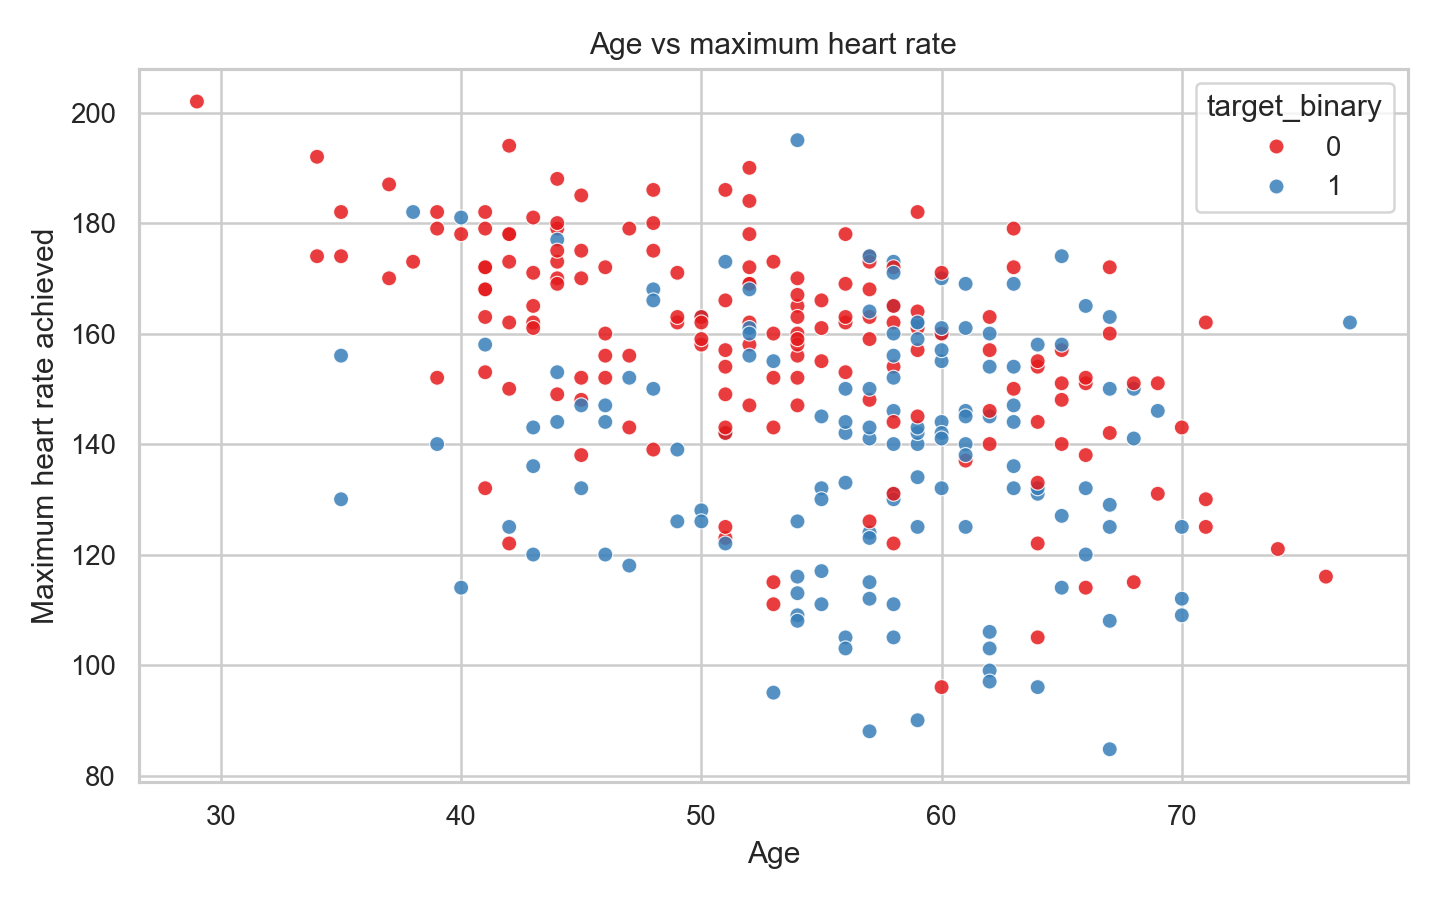
\includegraphics[width=\textwidth]{../outputs/figures/heart_disease_age_thalach_scatter.png}
    \caption{Tuổi và nhịp tim tối đa}
\end{subfigure}
\caption[Minh họa Heart Disease]{Minh họa Heart Disease. Python source: \texttt{src/analyze\_heart\_disease.py}; figure paths: \texttt{outputs/figures/heart\_disease\_target\_distribution.png}, \texttt{outputs/figures/heart\_disease\_age\_thalach\_scatter.png}.}
\label{fig:chapter2_heart_disease}
\end{figure}

\textbf{Kết quả ban đầu.} Bảng tần suất cho thấy target có hai nhóm chính sau khi quy về nhị phân: không bệnh và có bệnh. Baseline ở Bảng \ref{tab:chapter2_ml_preview} đạt F1 = 0.897 với Random Forest, cao hơn Logistic Regression và gần với SVM RBF. Hình \ref{fig:chapter2_heart_disease} minh họa mất cân bằng nhẹ của target và quan hệ giữa tuổi, \texttt{thalach} và nhãn bệnh.

\subsection{A2 - CDC Diabetes Health Indicators}

\textbf{Nguồn gốc và cấu trúc dữ liệu.} CDC Diabetes Health Indicators là bộ dữ liệu dạng bảng từ UCI, được lưu tại \path{datasets/uci_891_cdc_diabetes_health_indicators/}. Dữ liệu có 253,680 mẫu, 21 features và 1 target là \texttt{Diabetes\_binary}. Mỗi dòng biểu diễn một người trả lời khảo sát sức khỏe; các biến mô tả bệnh nền, hành vi sống, khả năng tiếp cận y tế, tự đánh giá sức khỏe và nhân khẩu học.

\textbf{Trường dữ liệu và phân phối.} Target \texttt{Diabetes\_binary} mất cân bằng rõ: 218,334 mẫu lớp 0 (86.07\%) và 35,346 mẫu lớp 1 (13.93\%). Nhóm bệnh nền gồm \texttt{HighBP}, \texttt{HighChol}, \texttt{Stroke}; nhóm hành vi gồm \texttt{Smoker}, \texttt{PhysActivity}, \texttt{Fruits}, \texttt{Veggies}; nhóm tự đánh giá gồm \texttt{GenHlth}, \texttt{MentHlth}, \texttt{PhysHlth}; nhóm xã hội học gồm \texttt{Sex}, \texttt{Age}, \texttt{Education}, \texttt{Income}. BMI có trung bình 28.38, trung vị 27 và khoảng giá trị thô 12--98; sau xử lý outlier, khoảng hợp lý hơn là 13.5--41.5. \texttt{MentHlth} và \texttt{PhysHlth} có trung vị 0 nhưng có giá trị cực đại 30 ngày, cho thấy phân phối lệch phải: phần lớn người trả lời không báo cáo ngày sức khỏe kém, nhưng một nhóm nhỏ có tình trạng kéo dài. \texttt{Age} có trung bình mã hóa 8.03, \texttt{Income} trung bình 6.05; đây là các biến ordinal nên không nên diễn giải như đại lượng liên tục tuyệt đối.

\textbf{Tổng quan bài báo liên quan.} Nguồn gốc dữ liệu gắn với hệ thống BRFSS của CDC, một khảo sát quy mô lớn về hành vi, bệnh nền và yếu tố nhân khẩu học trong cộng đồng \cite{CDC2023BRFSS}. Smith và cộng sự đóng gói bộ diabetes health indicators thành bài toán phân loại nguy cơ tiểu đường dựa trên dữ liệu tự báo cáo, giúp dữ liệu dễ dùng trong UCI/Kaggle và các thí nghiệm học máy \cite{Smith2014CDCIndicators}. Các nghiên cứu liên quan thường tóm tắt mục tiêu là phát hiện nhóm nguy cơ cao từ BMI, huyết áp, cholesterol, hoạt động thể chất, tuổi và thu nhập; kết quả đạt được là chứng minh dữ liệu khảo sát có thể dùng cho dự đoán sàng lọc, dù nhiễu do tự báo cáo và mất cân bằng lớp làm bài toán khó hơn dữ liệu y khoa đo trực tiếp. Điều này phù hợp với báo cáo hiện tại: mô hình đạt F1 trung bình khá, nhưng cần cân bằng lớp và đánh giá bằng recall/F1 thay vì chỉ accuracy.

\begin{table}[H]
\centering
\caption{Nhóm biến tiêu biểu trong CDC Diabetes}
\label{tab:cdc_feature_groups}
\small
\begin{tabular}{lll}
\toprule
Nhóm biến & Biến tiêu biểu & Ý nghĩa phân tích \\
\midrule
Bệnh nền & HighBP, HighChol, Stroke & Tình trạng sức khỏe nền \\
Hành vi & Smoker, PhysActivity, Fruits, Veggies & Lối sống và nguy cơ \\
Tiếp cận y tế & AnyHealthcare, NoDocbcCost & Khả năng chăm sóc sức khỏe \\
Tự đánh giá & GenHlth, MentHlth, PhysHlth & Sức khỏe tự báo cáo \\
Nhân khẩu & Sex, Age, Education, Income & Yếu tố xã hội học \\
\bottomrule
\end{tabular}
\end{table}

\begin{table}[H]
\centering
\caption{Thống kê mô tả các thuộc tính chính của CDC Diabetes}
\label{tab:cdc_descriptive_stats}
\small
\begin{tabular}{lllll}
\toprule
Thuộc tính & Loại & Trung bình & Độ phân tán & Ghi chú \\
\midrule
BMI & Liên tục & 28.38 & std = 6.61 & Lệch phải \\
GenHlth & Thứ bậc & 2.51 & std = 1.07 & Tự đánh giá sức khỏe \\
MentHlth & Rời rạc & 3.18 & std = 7.41 & Nhiều giá trị 0 \\
PhysHlth & Rời rạc & 4.24 & std = 8.72 & Nhiều giá trị 0 \\
Age & Thứ bậc & 8.03 & std = 3.05 & Mã nhóm tuổi \\
Income & Thứ bậc & 6.05 & std = 2.07 & Mã nhóm thu nhập \\
\bottomrule
\end{tabular}
\end{table}

\begin{figure}[H]
\centering
\begin{subfigure}{0.92\textwidth}
    \centering
    \includegraphics[width=\textwidth]{../outputs/figures/cdc_diabetes_target_distribution.png}
    \caption{Phân phối Diabetes\_binary}
\end{subfigure}

\vspace{0.4cm}

\begin{subfigure}{0.92\textwidth}
    \centering
    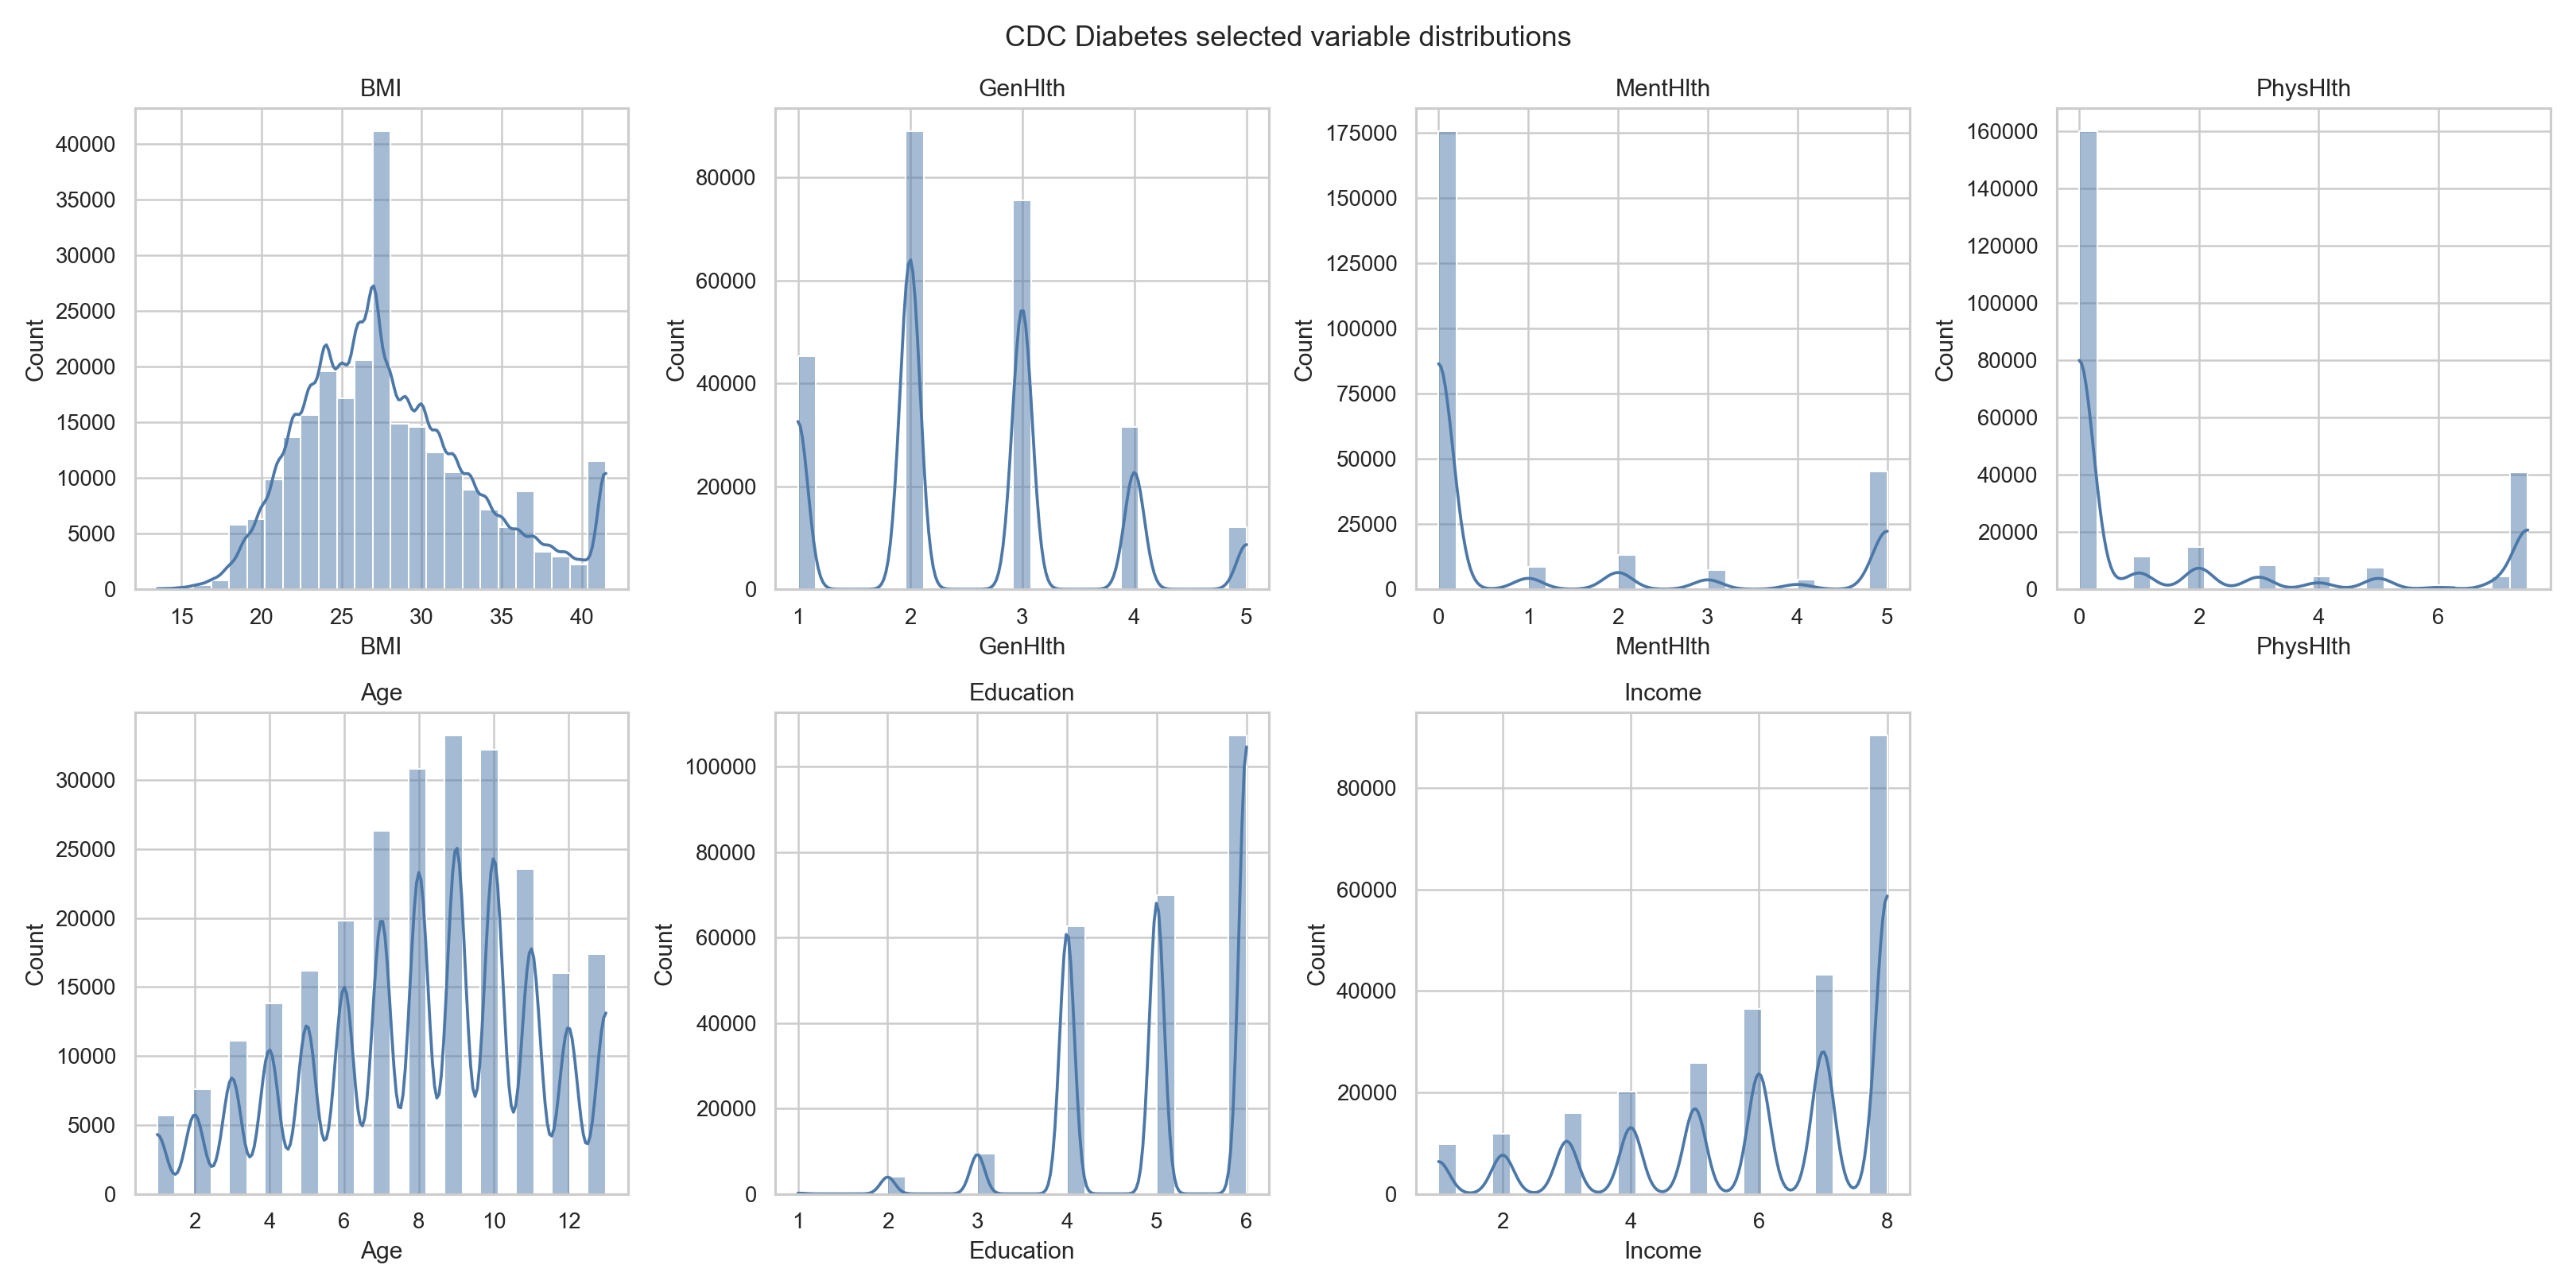
\includegraphics[width=\textwidth]{../outputs/figures/cdc_diabetes_selected_histograms.png}
    \caption{Histogram các biến sức khỏe}
\end{subfigure}
\caption[Minh họa CDC Diabetes]{Minh họa CDC Diabetes Health Indicators. Python source: \texttt{src/analyze\_cdc\_diabetes.py}; figure paths: \texttt{outputs/figures/cdc\_diabetes\_target\_distribution.png}, \texttt{outputs/figures/cdc\_diabetes\_selected\_histograms.png}. Bảng minh chứng bổ sung: \texttt{outputs/tables/cdc\_diabetes\_preprocessing\_comparison.csv}, \texttt{outputs/tables/cdc\_diabetes\_evidence\_index.csv}.}
\label{fig:chapter2_cdc_diabetes}
\end{figure}

\textbf{Kết quả ban đầu.} Dữ liệu có quy mô lớn nên phù hợp để kiểm tra ổn định của mô hình trên dữ liệu bảng nhiều biến ordinal/nhị phân. Baseline tốt nhất trong mẫu thử đạt F1 = 0.761 với SVM RBF, trong khi Logistic Regression đạt accuracy = 0.744. Hình \ref{fig:chapter2_cdc_diabetes} cho thấy target không cân bằng hoàn toàn và các biến như BMI, tuổi, sức khỏe tổng quát có phân phối lệch, cần chuẩn hóa hoặc biến đổi khi mô hình yêu cầu. Phân tích bổ sung theo mẫu Heart Disease được lưu trong \texttt{src/analyze\_cdc\_diabetes.py}; các bảng \texttt{cdc\_diabetes\_summary.csv}, \texttt{cdc\_diabetes\_preprocessing\_comparison.csv} và \texttt{cdc\_diabetes\_evidence\_index.csv} ghi lại đầy đủ thống kê mô tả, so sánh trước--sau xử lý và đường dẫn minh chứng.

\subsection{A3 - Breast Cancer Wisconsin Diagnostic}

\textbf{Nguồn gốc và cấu trúc dữ liệu.} Breast Cancer Wisconsin Diagnostic là bộ dữ liệu chẩn đoán ung thư vú từ UCI, được lưu tại \path{datasets/uci_17_breast_cancer_wisconsin_diagnostic/}. Bộ dữ liệu có 569 mẫu, 30 features và target \texttt{Diagnosis}. Target có hai lớp: malignant (M) và benign (B), tương ứng khối u ác tính và lành tính.

\textbf{Trường dữ liệu và phân phối.} Các features là đặc trưng hình học/kết cấu của nhân tế bào: radius, texture, perimeter, area, smoothness, compactness, concavity, concave points, symmetry và fractal dimension; mỗi nhóm có ba dạng mean, standard error và worst value. Phân phối lớp gồm 357 mẫu benign (62.74\%) và 212 mẫu malignant (37.26\%), không cân bằng hoàn toàn nhưng vẫn đủ mẫu cho cả hai lớp. \texttt{radius1} có trung bình 14.13 và trung vị 13.37; \texttt{area1} có trung bình 654.89, trung vị 551.1 và phương sai lớn, cho thấy kích thước khối u có outlier. Sau xử lý, \texttt{area1} được chặn từ max 2501 xuống 1326.3 và \texttt{radius1} từ 28.11 xuống 21.9. \texttt{concavity1} có trung vị 0.06154 nhưng max 0.4268, phản ánh độ lõm là biến phân biệt quan trọng giữa hai lớp. Heatmap cho thấy các biến radius, perimeter và area tương quan cao, vì vậy có thể cần chuẩn hóa và kiểm tra đa cộng tuyến trước khi dùng mô hình tuyến tính.

\textbf{Tổng quan bài báo liên quan.} Street, Wolberg và Mangasarian xây dựng bộ dữ liệu từ ảnh fine needle aspirate (FNA), sau đó trích xuất đặc trưng số mô tả nhân tế bào để chẩn đoán u lành/ác \cite{Street1993NuclearFeatures}. Điểm chính của bài báo là biến ảnh y sinh thành vector đặc trưng định lượng, giúp mô hình học máy có thể xử lý mà không cần ảnh gốc. Mangasarian và cộng sự tiếp tục khai thác hướng tối ưu hóa và separating hyperplane cho phân lớp ung thư vú \cite{Mangasarian1995BreastCancer}. Kết quả/ý nghĩa đạt được của các nghiên cứu này là chứng minh đặc trưng hình học của nhân tế bào có tính phân tách mạnh; trong báo cáo hiện tại, điều này được xác nhận khi SVM RBF đạt F1 = 0.976, cao nhất trong nhóm A.

\begin{table}[H]
\centering
\caption{Danh sách feature tiêu biểu của Breast Cancer}
\label{tab:breast_feature_dictionary}
\small
\begin{tabular}{llll}
\toprule
Nhóm feature & Loại & Ý nghĩa thực tế & Ví dụ \\
\midrule
radius/perimeter/area & Liên tục & Kích thước nhân tế bào & radius1, area1 \\
texture & Liên tục & Độ biến thiên cường độ ảnh & texture1 \\
smoothness/compactness & Liên tục & Hình dạng biên nhân & smoothness1 \\
concavity/concave points & Liên tục & Độ lõm và điểm lõm biên & concavity1 \\
symmetry/fractal dimension & Liên tục & Đối xứng và độ phức tạp biên & symmetry1 \\
Diagnosis & Định tính & Nhãn lành/ác tính & B, M \\
\bottomrule
\end{tabular}
\end{table}

\begin{table}[H]
\centering
\caption{Thống kê mô tả các thuộc tính chính của Breast Cancer}
\label{tab:breast_descriptive_stats}
\small
\begin{tabular}{lllll}
\toprule
Thuộc tính & Loại & Trung bình & Độ phân tán & Ghi chú \\
\midrule
radius1 & Liên tục & 14.13 & std = 3.52 & Kích thước nhân \\
texture1 & Liên tục & 19.29 & std = 4.30 & Kết cấu \\
area1 & Liên tục & 654.89 & std = 351.91 & Phân tán lớn \\
concavity1 & Liên tục & 0.09 & std = 0.08 & Biến phân biệt mạnh \\
Diagnosis & Định tính & -- & B/M = 357/212 & Target \\
\bottomrule
\end{tabular}
\end{table}

\begin{figure}[H]
\centering
\begin{subfigure}{0.92\textwidth}
    \centering
    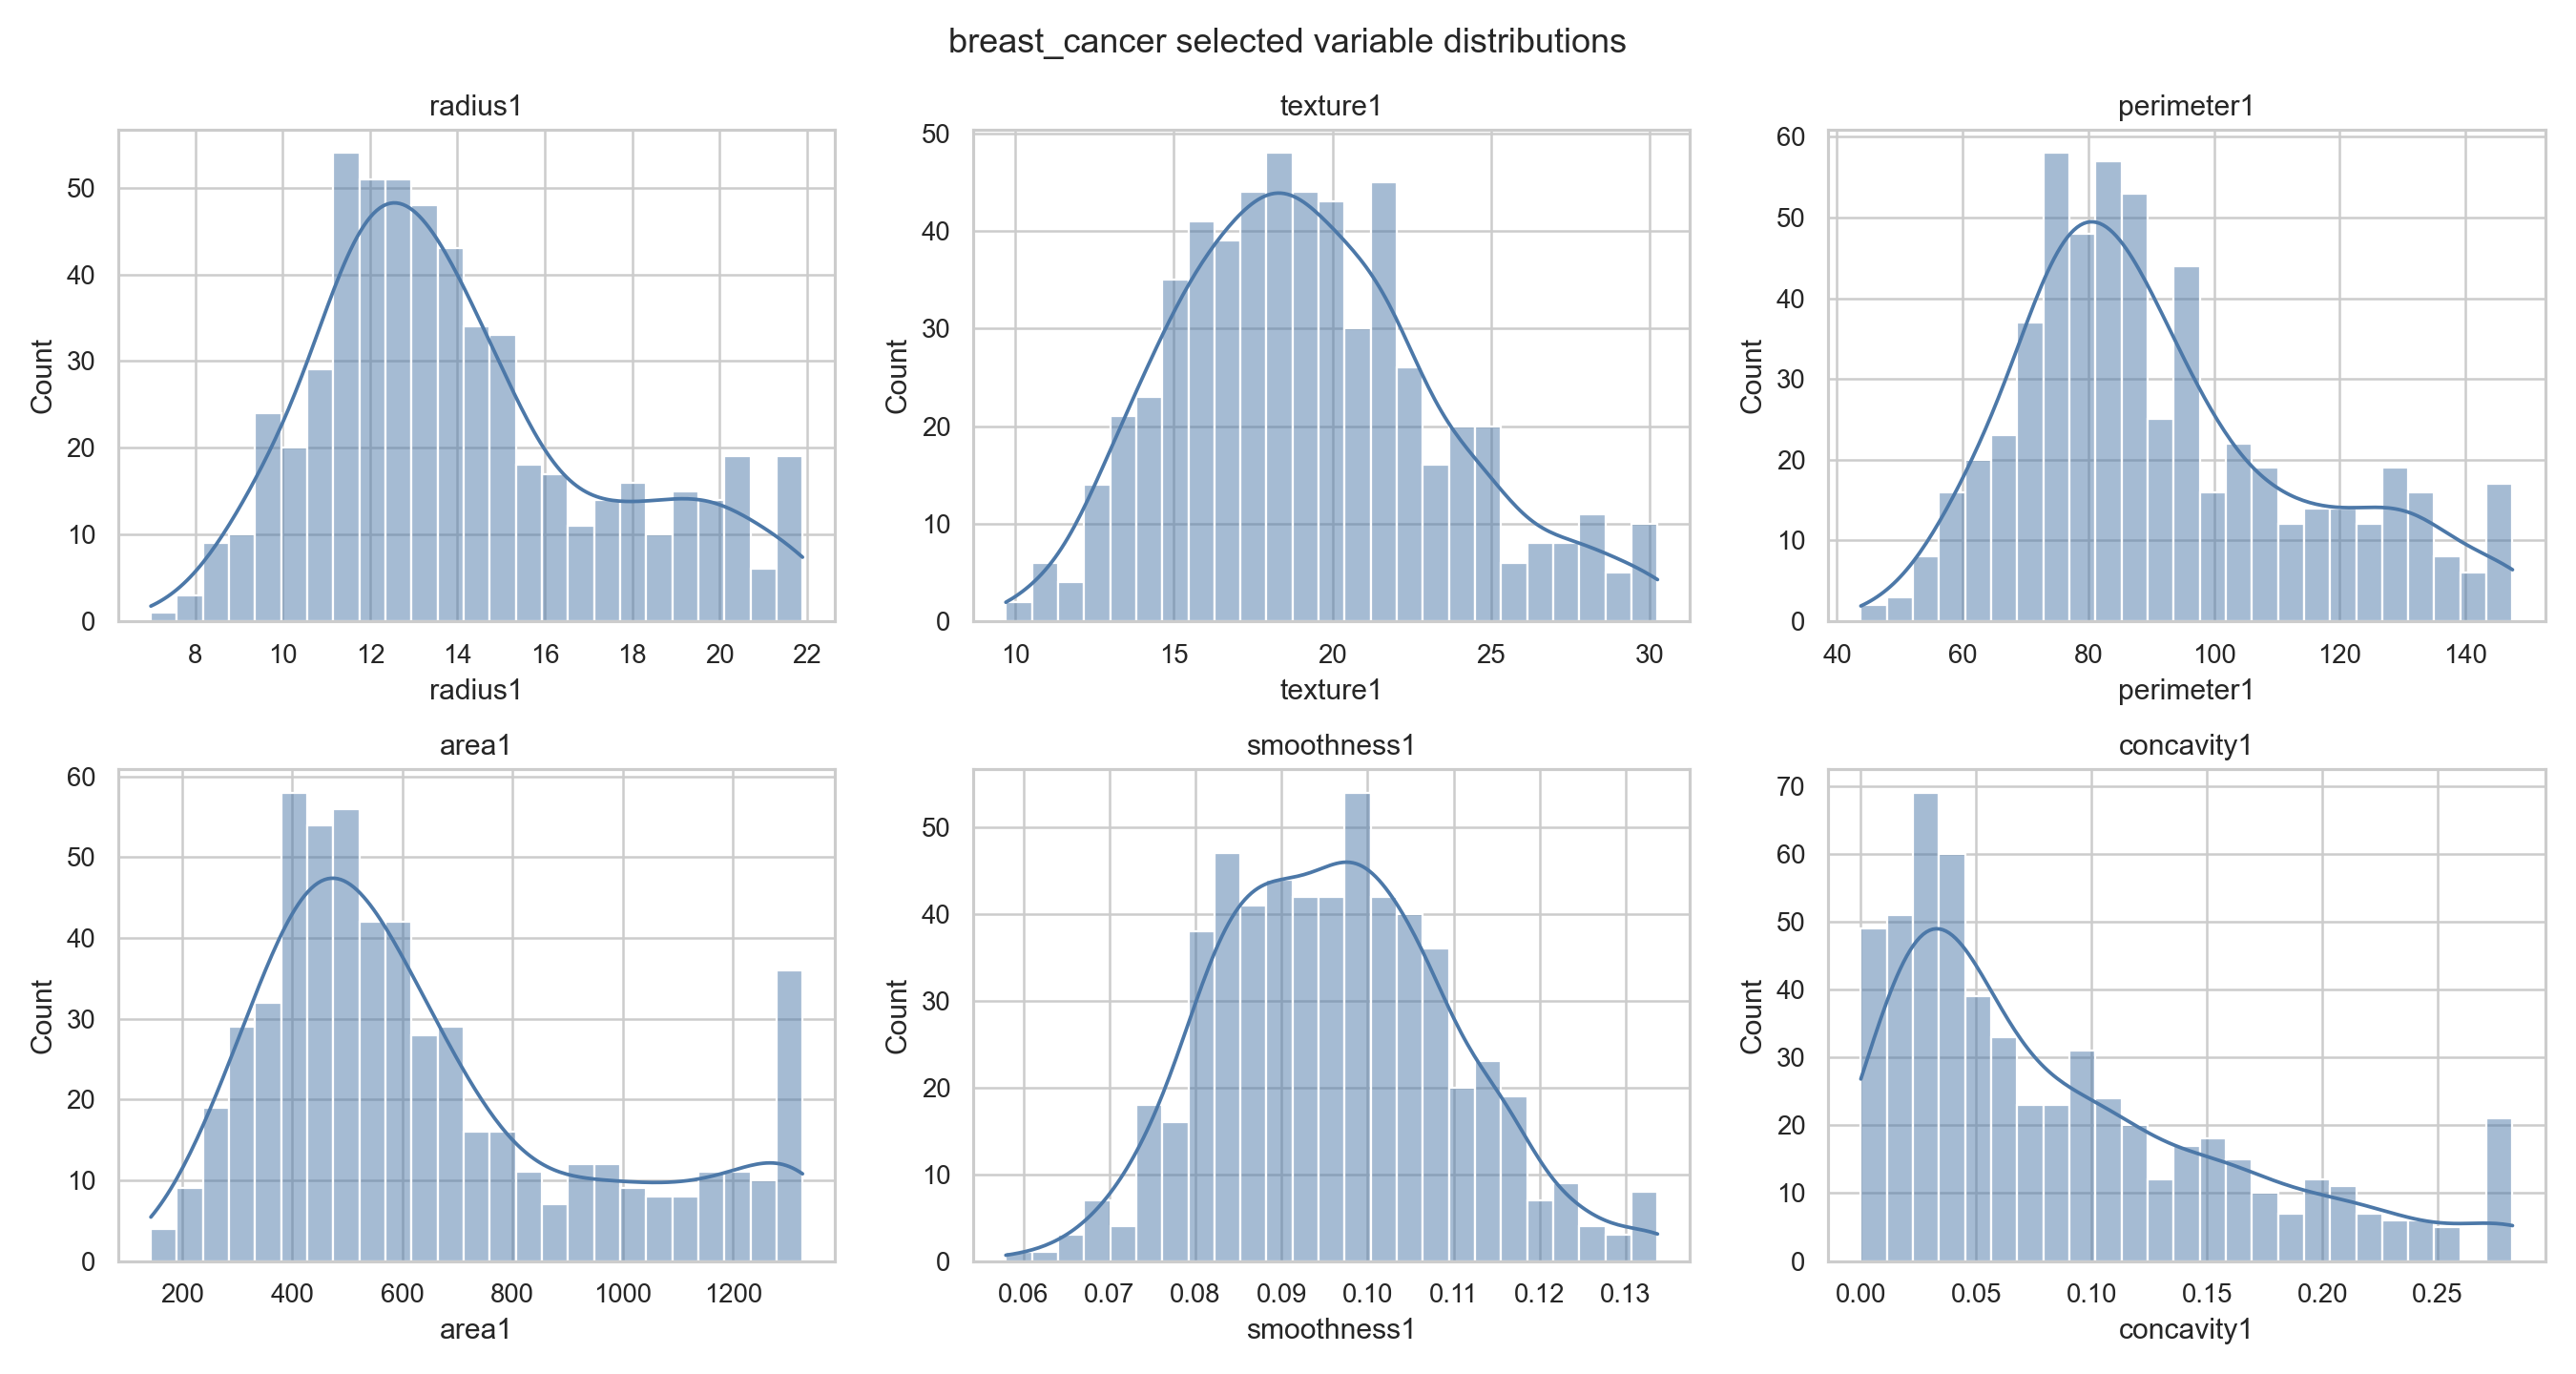
\includegraphics[width=\textwidth]{../outputs/figures/breast_cancer_selected_histograms.png}
    \caption{Histogram các biến chọn}
\end{subfigure}

\vspace{0.4cm}

\begin{subfigure}{0.92\textwidth}
    \centering
    \includegraphics[width=\textwidth]{../outputs/figures/breast_cancer_correlation_heatmap.png}
    \caption{Heatmap tương quan}
\end{subfigure}
\caption[Minh họa cấu trúc số của Breast Cancer]{Minh họa cấu trúc số của Breast Cancer Wisconsin Diagnostic. Python source: \texttt{src/analyze\_tabular\_health.py}; figure paths: \texttt{outputs/figures/breast\_cancer\_selected\_histograms.png}, \texttt{outputs/figures/breast\_cancer\_correlation\_heatmap.png}.}
\label{fig:chapter2_breast_numeric}
\end{figure}

\textbf{Lý do chọn biểu đồ.} Histogram giúp xem hình dạng phân phối của các biến hình học; heatmap giúp phát hiện các nhóm biến tương quan cao trong Breast Cancer.

\textbf{Nhận xét.} Hình \ref{fig:chapter2_breast_numeric} cho thấy bộ Breast Cancer có nhiều biến liên tục và tương quan cao giữa các phép đo hình học. Điều này giải thích vì sao các mô hình tuyến tính sau chuẩn hóa, như Logistic Regression hoặc SVM, thường hoạt động tốt trên bộ dữ liệu này.

\textbf{Kết quả ban đầu.} Baseline SVM RBF đạt accuracy = 0.982 và F1 = 0.976, cao nhất trong ba bộ dữ liệu bảng nhóm A. Kết quả này phù hợp với nhận xét từ heatmap: nhiều đặc trưng hình học có khả năng phân tách rõ giữa malignant và benign.

\section{Nhóm B: Dữ liệu chuỗi thời gian và cảm biến}

Nhóm B gồm các bộ dữ liệu có yếu tố thứ tự thời gian hoặc tín hiệu cảm biến. Điểm khác biệt so với dữ liệu bảng là quan sát hiện tại có thể phụ thuộc vào thời điểm trước đó, nên cần mô tả tần suất thu thập, cửa sổ tín hiệu và cách tách train/test theo thời gian.

\begin{table}[H]
\centering
\caption{Tổng hợp đặc trưng chuỗi thời gian của nhóm B}
\label{tab:group_b_timeseries_summary}
\small
\begin{tabular}{p{0.18\textwidth}p{0.12\textwidth}p{0.14\textwidth}p{0.18\textwidth}p{0.24\textwidth}}
\toprule
Dataset & Số mẫu & Features & Tần suất/cửa sổ & Ý nghĩa chuỗi thời gian \\
\midrule
B1 Appliances & 19735 & 28 & 10 phút/mẫu & Dự báo tiêu thụ năng lượng theo thời gian \\
B2 HAR & 10299 & 561 & Cửa sổ tín hiệu inertial & Nhận dạng hoạt động từ chuỗi gia tốc/gyro \\
B3 MHEALTH & 1215745 & 23 & Log cảm biến liên tục & Chuyển log đa kênh thành cửa sổ hoạt động \\
\bottomrule
\end{tabular}
\end{table}

\subsection{B1 - Appliances Energy Prediction}

\textbf{Nguồn gốc và cấu trúc dữ liệu.} Appliances Energy Prediction là bộ dữ liệu UCI được lưu tại \path{datasets/uci_374_appliances_energy_prediction/}. Bộ dữ liệu có 19,735 mẫu, 28 features và target \texttt{Appliances}. Mỗi mẫu gắn với một mốc thời gian cách nhau khoảng 10 phút; khoảng quan sát bắt đầu từ 2016-01-11 17:00:00 đến 2016-05-27 18:00:00.

\textbf{Trường dữ liệu và phân phối.} Các features bao gồm nhiệt độ, độ ẩm trong nhiều khu vực, ánh sáng, áp suất, độ ẩm ngoài trời, tốc độ gió, tầm nhìn và điểm sương. Target \texttt{Appliances} có trung bình 97.69, trung vị 60, mode 50, độ lệch chuẩn 102.52 và hệ số biến thiên khoảng 1.05; max 1080 cho thấy phân phối lệch phải mạnh. Biến \texttt{lights} có trung vị và phân vị 75 đều bằng 0, nghĩa là phần lớn thời điểm đèn không tiêu thụ hoặc không được ghi nhận ở mức đáng kể. \texttt{T1} có trung bình 21.69, \texttt{RH\_1} trung bình 40.26 và \texttt{T\_out} trung bình 7.41, phản ánh đồng thời điều kiện trong nhà và ngoài trời. Vì đây là dữ liệu chuỗi thời gian, việc chia train/test phải theo thứ tự thời gian; nếu tách ngẫu nhiên sẽ làm rò rỉ thông tin tương lai và đánh giá mô hình quá lạc quan.

\textbf{Tổng quan bài báo liên quan.} Candanedo, Feldheim và Deramaix giới thiệu bộ dữ liệu này để dự báo tiêu thụ năng lượng thiết bị gia dụng từ cảm biến trong nhà và dữ liệu thời tiết \cite{Candanedo2017Appliances}. Bài báo gốc so sánh nhiều mô hình hồi quy, trong đó Random Forest đạt hiệu quả tốt nhờ mô hình hóa được quan hệ phi tuyến giữa nhiệt độ, độ ẩm, ánh sáng, điều kiện thời tiết và hành vi sử dụng thiết bị. Kết quả chính của nghiên cứu là chỉ ra dữ liệu cảm biến môi trường có thể dùng để dự báo năng lượng ở quy mô hộ gia đình, nhưng cần đặc trưng thời gian như giờ, ngày trong tuần, lag, rolling mean và rolling standard deviation. Trong báo cáo này, mô hình tuyến tính ban đầu có R2 thấp, xác nhận rằng nếu chưa tạo đặc trưng chuỗi thời gian thì mô hình khó khai thác đầy đủ mùa vụ và thói quen sinh hoạt.

\begin{table}[H]
\centering
\caption{Thống kê mô tả các thuộc tính chính của Appliances Energy}
\label{tab:appliances_descriptive_stats}
\small
\begin{tabular}{lllll}
\toprule
Thuộc tính & Loại & Trung bình & Độ phân tán & Ghi chú \\
\midrule
Appliances & Liên tục & 97.69 & std = 102.52 & Target lệch phải \\
lights & Liên tục & 3.80 & std = 7.94 & Nhiều giá trị 0 \\
T1 & Liên tục & 21.69 & std = 1.61 & Nhiệt độ trong nhà \\
RH\_1 & Liên tục & 40.26 & std = 3.98 & Độ ẩm trong nhà \\
T\_out & Liên tục & 7.41 & std = 5.32 & Nhiệt độ ngoài trời \\
Windspeed & Liên tục & 4.04 & std = 2.45 & Thời tiết \\
\bottomrule
\end{tabular}
\end{table}

\begin{figure}[H]
\centering
\begin{subfigure}{0.92\textwidth}
    \centering
    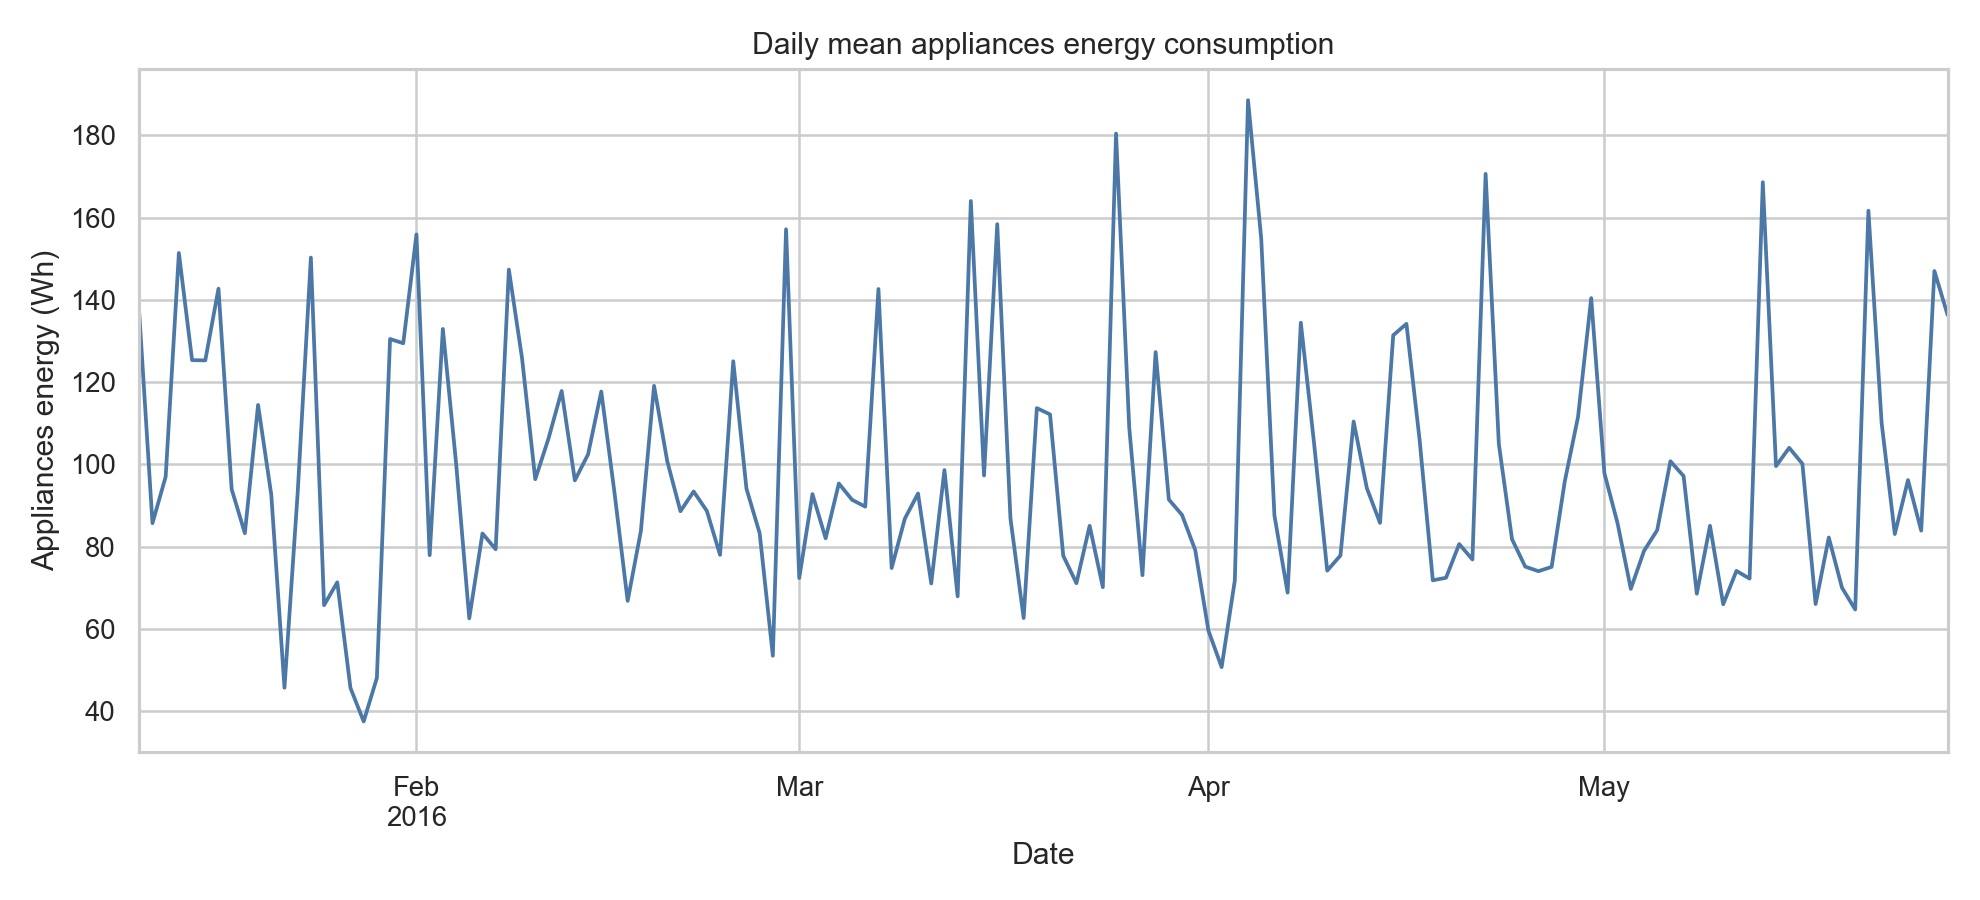
\includegraphics[width=\textwidth]{../outputs/figures/appliances_energy_daily_line.png}
    \caption{Tiêu thụ trung bình theo ngày}
\end{subfigure}

\vspace{0.4cm}

\begin{subfigure}{0.92\textwidth}
    \centering
    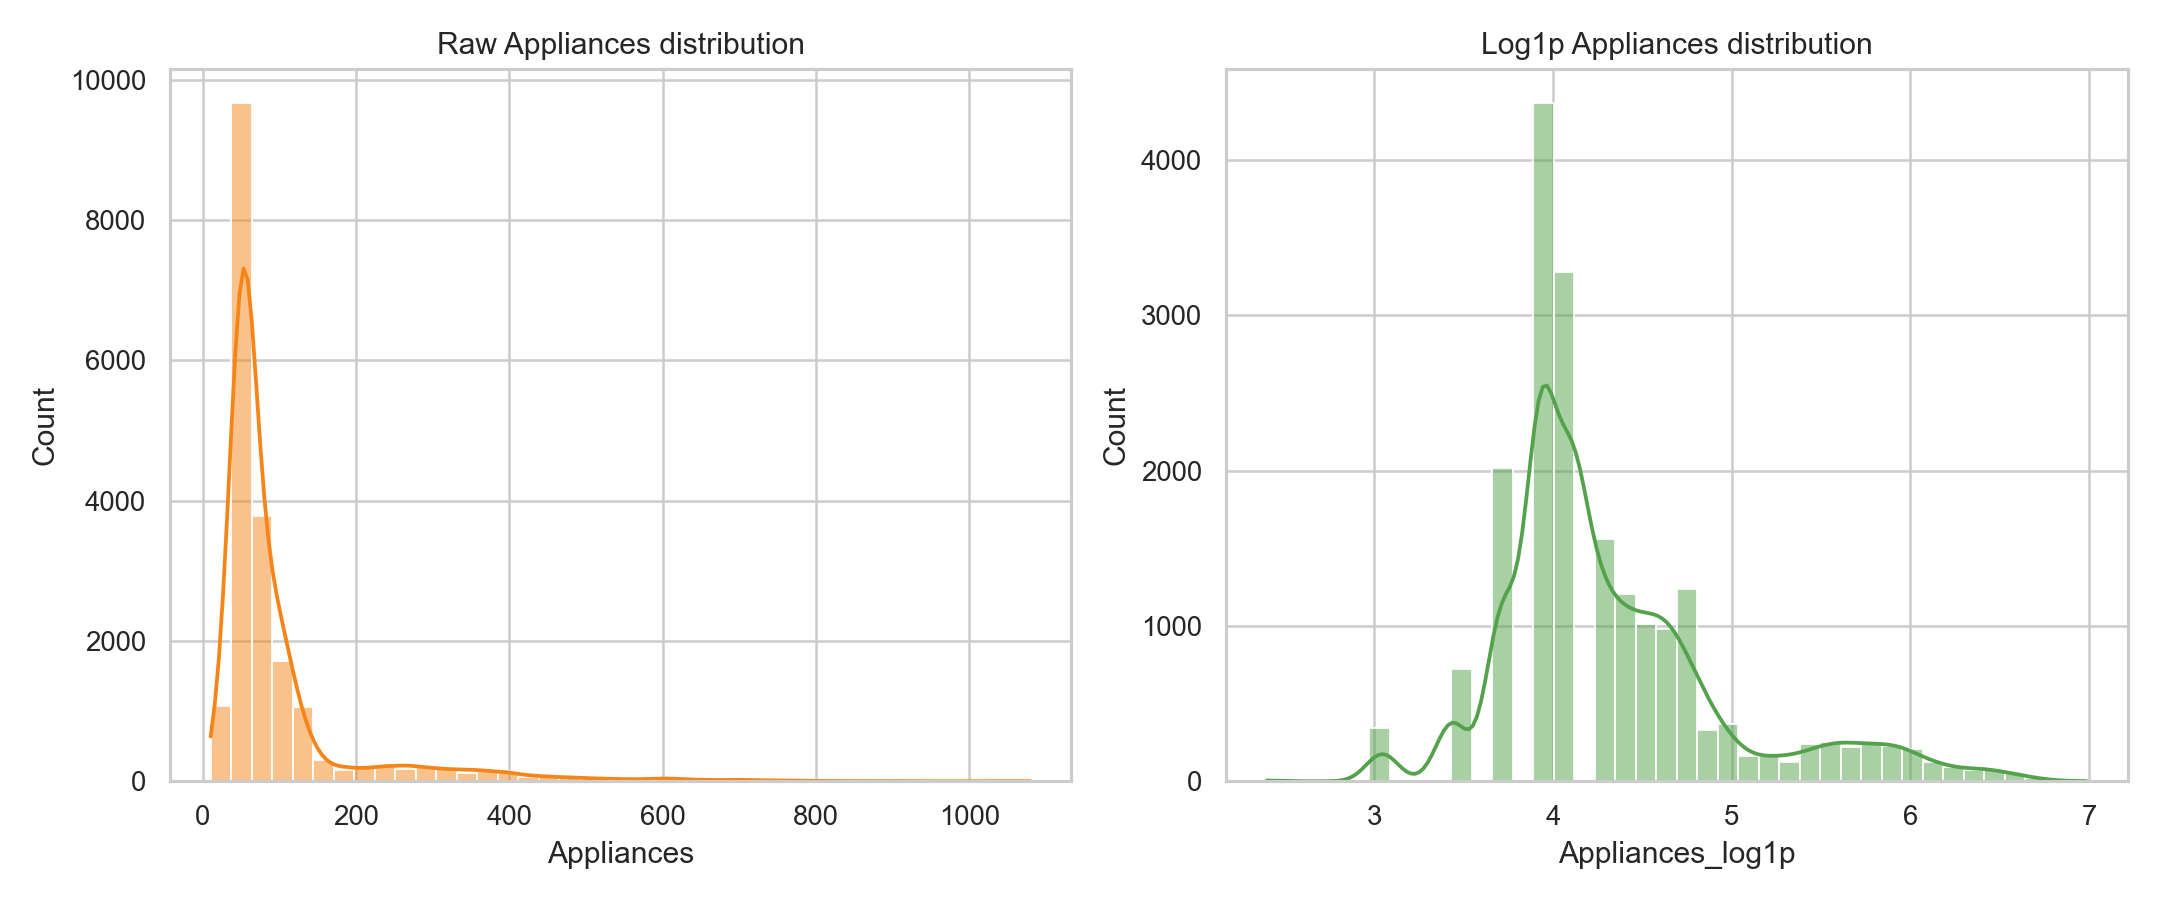
\includegraphics[width=\textwidth]{../outputs/figures/appliances_energy_distribution_raw_vs_log.png}
    \caption{Phân phối target trước/sau log}
\end{subfigure}
\caption[Minh họa đặc trưng chuỗi thời gian của Appliances Energy]{Minh họa đặc trưng chuỗi thời gian của Appliances Energy. Python source: \texttt{src/analyze\_appliances\_energy.py}; figure paths: \texttt{outputs/figures/appliances\_energy\_daily\_line.png}, \texttt{outputs/figures/appliances\_energy\_distribution\_raw\_vs\_log.png}.}
\label{fig:chapter2_appliances_timeseries}
\end{figure}

\textbf{Lý do chọn biểu đồ.} Line chart được chọn vì Appliances Energy là dữ liệu chuỗi thời gian; histogram raw-vs-log được chọn để kiểm tra mức lệch phải của target và tác dụng của log transform.

\textbf{Nhận xét.} Hình \ref{fig:chapter2_appliances_timeseries} cho thấy dữ liệu Appliances có biến động theo thời gian và phân phối target lệch phải. Do đó, ngoài các mô hình regression thông thường, các đặc trưng lag, rolling mean và log transform có thể cần thiết để cải thiện kết quả dự báo.

\textbf{Kết quả ban đầu.} Khi tách train/test theo thứ tự thời gian, Linear Regression đạt MAE = 58.71 và RMSE = 89.40. Random Forest chưa tốt trong cấu hình ban đầu vì chưa bổ sung đủ đặc trưng lag/rolling, cho thấy bài toán dự báo năng lượng cần xử lý seasonality và đặc trưng thời gian cẩn thận hơn classification dữ liệu bảng.

\subsection{B2 - Human Activity Recognition Using Smartphones}

\textbf{Nguồn gốc và cấu trúc dữ liệu.} Human Activity Recognition Using Smartphones (HAR) là bộ dữ liệu cảm biến chuyển động từ UCI, được giải nén tại \path{datasets/human+activity+recognition+using+smartphones/UCI HAR Dataset/}. Bộ dữ liệu có 10,299 mẫu, 561 features và 6 nhãn hoạt động: walking, walking upstairs, walking downstairs, sitting, standing và laying. Dữ liệu gồm feature vectors đã xử lý và tín hiệu inertial raw trong thư mục train/test.

\textbf{Trường dữ liệu và phân phối.} 561 features được trích từ accelerometer và gyroscope, bao gồm đặc trưng miền thời gian, miền tần số, trung bình, độ lệch chuẩn, năng lượng, entropy, tương quan giữa trục và dominant frequency. Phân phối lớp tương đối cân bằng: LAYING 1,944 mẫu (18.88\%), STANDING 1,906 (18.51\%), SITTING 1,777 (17.25\%), WALKING 1,722 (16.72\%), WALKING\_UPSTAIRS 1,544 (14.99\%) và WALKING\_DOWNSTAIRS 1,406 (13.65\%). Nhóm hoạt động tĩnh (sitting, standing, laying) và nhóm hoạt động động (walking, upstairs, downstairs) có mẫu dao động cảm biến khác nhau; đây là cơ sở để boxplot theo activity cho thấy khả năng phân tách trước khi huấn luyện mô hình.

\textbf{Tổng quan bài báo liên quan.} Anguita và cộng sự công bố HAR như benchmark nhận dạng hoạt động bằng smartphone, sử dụng cảm biến gia tốc và con quay hồi chuyển thu thập trên cửa sổ tín hiệu cố định \cite{Anguita2013HAR}. Bài báo tóm tắt quy trình từ tín hiệu raw, lọc nhiễu, trích xuất 561 đặc trưng rồi huấn luyện SVM để phân loại sáu hoạt động. Kết quả/ý nghĩa đạt được là chứng minh điện thoại thông minh có thể thay thế thiết bị chuyên dụng trong activity recognition, đồng thời cung cấp bộ feature vector chuẩn cho so sánh mô hình. Với báo cáo hiện tại, phân phối lớp khá cân bằng giúp classification/clustering đáng tin cậy hơn MHEALTH, còn tín hiệu raw mở ra hướng dùng CNN 1D hoặc LSTM nếu mở rộng sang học sâu.

\begin{table}[H]
\centering
\caption{Cấu trúc nhãn hoạt động trong HAR}
\label{tab:har_activity_labels}
\small
\begin{tabular}{ll}
\toprule
Mã nhãn & Hoạt động \\
\midrule
1 & WALKING \\
2 & WALKING\_UPSTAIRS \\
3 & WALKING\_DOWNSTAIRS \\
4 & SITTING \\
5 & STANDING \\
6 & LAYING \\
\bottomrule
\end{tabular}
\end{table}

\begin{table}[H]
\centering
\caption{Thống kê mô tả các thuộc tính chính của HAR}
\label{tab:har_descriptive_stats}
\small
\begin{tabular}{lllll}
\toprule
Thuộc tính & Loại & Trung bình & Độ phân tán & Ghi chú \\
\midrule
f001\_tBodyAcc-mean()-X & Liên tục & 0.27 & std = 0.07 & Gia tốc trục X \\
f004\_tBodyAcc-std()-X & Liên tục & -0.61 & std = 0.45 & Dao động tín hiệu \\
f121\_tBodyGyro-mean()-X & Liên tục & -0.03 & std = 0.13 & Gyro trục X \\
activity & Định tính & -- & 6 lớp & Target khá cân bằng \\
subject & Định tính & -- & 30 người & Nhóm quan sát \\
\bottomrule
\end{tabular}
\end{table}

\begin{figure}[H]
\centering
\begin{subfigure}{0.92\textwidth}
    \centering
    \includegraphics[width=\textwidth]{../outputs/figures/har_activity_distribution.png}
    \caption{Phân phối activity}
\end{subfigure}

\vspace{0.4cm}

\begin{subfigure}{0.92\textwidth}
    \centering
    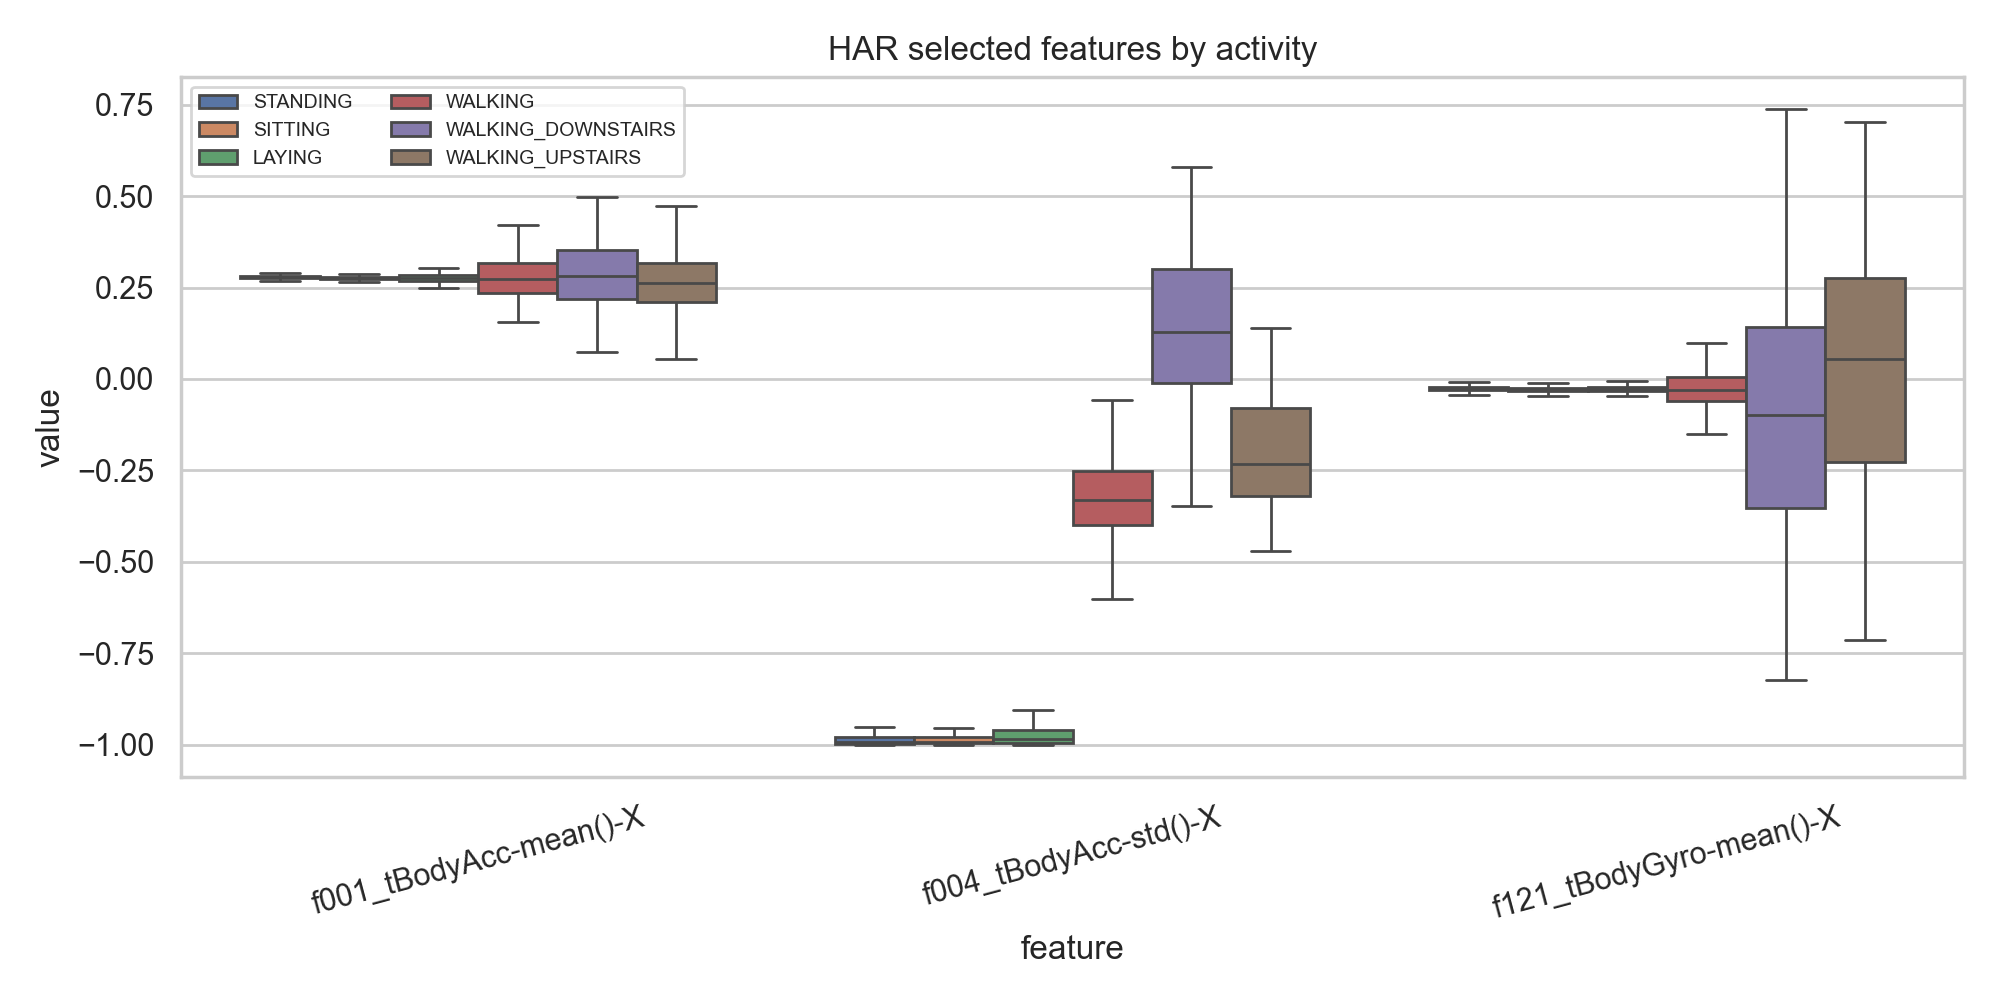
\includegraphics[width=\textwidth]{../outputs/figures/har_selected_feature_boxplot.png}
    \caption{Đặc trưng cảm biến theo activity}
\end{subfigure}
\caption[Minh họa HAR Smartphones]{Minh họa Human Activity Recognition Using Smartphones. Python source: \texttt{src/analyze\_har.py}; figure paths: \texttt{outputs/figures/har\_activity\_distribution.png}, \texttt{outputs/figures/har\_selected\_feature\_boxplot.png}.}
\label{fig:chapter2_har}
\end{figure}

\textbf{Kết quả ban đầu.} Hình \ref{fig:chapter2_har} cho thấy sáu hoạt động được ghi nhận tương đối đầy đủ, tạo điều kiện thuận lợi cho classification và clustering. Boxplot các đặc trưng gia tốc/gyro cho thấy một số hoạt động tĩnh và động có miền giá trị khác nhau, phù hợp với hướng dùng SVM, Random Forest hoặc CNN/LSTM trên tín hiệu raw.

\subsection{B3 - MHEALTH Dataset}

\textbf{Nguồn gốc và cấu trúc dữ liệu.} MHEALTH là bộ dữ liệu Mobile Health từ UCI, được lưu tại \path{datasets/MHEALTHDATASET/MHEALTHDATASET/}. Dữ liệu gồm 10 file subject log, tổng cộng 1,215,745 dòng, 23 features cảm biến và 1 cột activity label. Các cảm biến được đặt trên nhiều vị trí cơ thể, thu thập gia tốc, gyro, từ trường và tín hiệu liên quan sức khỏe.

\textbf{Trường dữ liệu và phân phối.} Mỗi dòng là một thời điểm trong log cảm biến, chưa phải một mẫu học máy độc lập theo nghĩa cửa sổ thời gian. Trong mẫu phân tích, nhãn NULL chiếm 282,379 dòng (70.59\%), lớn hơn nhiều so với các hoạt động thực như standing still 24,576 (6.14\%), sitting 21,568 (5.39\%), lying 18,496 (4.62\%), walking 16,960 (4.24\%), waist bends 13,684 (3.42\%) và climbing stairs 12,288 (3.07\%). Điều này cho thấy dữ liệu rất giàu về thời lượng ghi nhận nhưng mất cân bằng nghiêm trọng theo nhãn. Các trường \texttt{sensor\_01}--\texttt{sensor\_23} đại diện cho nhiều kênh đo; khi phân tích cần nhóm theo vị trí/cảm biến, chuẩn hóa scale, lọc nhãn NULL và chuyển log dài thành cửa sổ trượt có đặc trưng mean, variance, RMS, energy hoặc FFT.

\textbf{Tổng quan bài báo liên quan.} Banos và cộng sự xây dựng MHEALTH để đánh giá nhận dạng hoạt động và theo dõi sức khỏe bằng cảm biến đa vị trí trên cơ thể \cite{Banos2014MHEALTH}. Bài báo nhấn mạnh ưu điểm của dữ liệu đa kênh: cùng một hoạt động được quan sát từ nhiều vị trí cơ thể, giúp mô hình học được cả chuyển động cục bộ và toàn thân. Kết quả/ý nghĩa của nghiên cứu là cung cấp benchmark lớn cho activity recognition trong bối cảnh mobile health, nơi yêu cầu vừa nhận dạng hoạt động vừa hỗ trợ giám sát sức khỏe. Trong báo cáo này, phân phối NULL quá lớn cho thấy cần tiền xử lý mạnh hơn HAR: loại bỏ đoạn không hoạt động, cân bằng lớp và tạo cửa sổ trượt trước khi dùng SVM, Random Forest, CNN 1D hoặc LSTM.

\begin{table}[H]
\centering
\caption{So sánh hai bộ dữ liệu cảm biến nhóm B}
\label{tab:sensor_dataset_compare}
\small
\begin{tabular}{llll}
\toprule
Bộ dữ liệu & Số mẫu & Số đặc trưng & Điểm mạnh \\
\midrule
HAR & 10299 & 561 & Feature vector đã xử lý, nhãn hoạt động rõ \\
MHEALTH & 1215745 & 23 & Dữ liệu log dài, nhiều subject, cảm biến đa vị trí \\
\bottomrule
\end{tabular}
\end{table}

\begin{table}[H]
\centering
\caption{Thống kê mô tả các thuộc tính chính của MHEALTH}
\label{tab:mhealth_descriptive_stats}
\small
\begin{tabular}{lllll}
\toprule
Thuộc tính & Loại & Trung bình & Độ phân tán & Ghi chú \\
\midrule
sensor\_01 & Liên tục & -3.80 & std = 4.25 & Gia tốc/ngực \\
sensor\_02 & Liên tục & -9.44 & std = 3.30 & Gia tốc/ngực \\
sensor\_03 & Liên tục & 1.92 & std = 4.07 & Gia tốc/ngực \\
sensor\_10 & Liên tục & -0.34 & std = 0.57 & Kênh cảm biến khác \\
activity & Định tính & -- & NULL 70.59\% & Target mất cân bằng \\
\bottomrule
\end{tabular}
\end{table}

\begin{figure}[H]
\centering
\begin{subfigure}{0.92\textwidth}
    \centering
    \includegraphics[width=\textwidth]{../outputs/figures/mhealth_activity_distribution.png}
    \caption{Phân phối activity trên mẫu}
\end{subfigure}

\vspace{0.4cm}

\begin{subfigure}{0.92\textwidth}
    \centering
    \includegraphics[width=\textwidth]{../outputs/figures/mhealth_sensor_boxplot.png}
    \caption{Kênh cảm biến theo activity}
\end{subfigure}
\caption[Minh họa MHEALTH]{Minh họa MHEALTH Dataset. Python source: \texttt{src/analyze\_mhealth.py}; figure paths: \texttt{outputs/figures/mhealth\_activity\_distribution.png}, \texttt{outputs/figures/mhealth\_sensor\_boxplot.png}.}
\label{fig:chapter2_mhealth}
\end{figure}

\textbf{Kết quả ban đầu.} Hình \ref{fig:chapter2_mhealth} cho thấy dữ liệu MHEALTH có nhiều nhãn hoạt động và log cảm biến lớn. Hoạt động null chiếm nhiều dòng trong mẫu, vì vậy khi huấn luyện cần lọc hoặc cân bằng nhãn. Các kênh gia tốc ngực có phân phối khác nhau theo hoạt động, xác nhận dữ liệu phù hợp cho nhận dạng hoạt động bằng đặc trưng cửa sổ trượt.

\section{Nhóm C: Dữ liệu đa phương tiện}

Nhóm C chọn hai dạng dữ liệu đa phương tiện: ảnh và văn bản. Với nhóm này, mô tả không chỉ gồm số dòng mà còn phải nêu định dạng file gốc và cách chuyển dữ liệu thô thành đặc trưng số để thống kê/học máy.

\begin{table}[H]
\centering
\caption{Thông tin file gốc và đặc trưng trích xuất của nhóm C}
\label{tab:group_c_file_format_summary}
\small
\begin{tabular}{p{0.18\textwidth}p{0.14\textwidth}p{0.16\textwidth}p{0.20\textwidth}p{0.20\textwidth}}
\toprule
Dataset & Loại media & Số lượng & Định dạng gốc & Đặc trưng trích xuất \\
\midrule
C1 HAM10000 & Ảnh & 10015 ảnh & JPG + metadata CSV & width, height, mean/std intensity, dx \\
C2 Reuters & Văn bản & 21578 tài liệu & 22 file SGML & word count, char count, topic, TF-IDF \\
\bottomrule
\end{tabular}
\end{table}

\begin{table}[H]
\centering
\caption{Phương pháp trích xuất đặc trưng cho dữ liệu đa phương tiện}
\label{tab:group_c_feature_extraction_methods}
\small
\begin{tabular}{p{0.16\textwidth}p{0.22\textwidth}p{0.24\textwidth}p{0.24\textwidth}}
\toprule
Dataset & Truyền thống & Học sâu & Nghiên cứu liên quan \\
\midrule
HAM10000 & Histogram màu, texture, shape, ABCD & CNN, transfer learning ResNet/EfficientNet & Tschandl et al.; Esteva et al. \\
Reuters & Bag-of-words, TF-IDF, n-gram, chọn đặc trưng & Embedding, CNN/RNN, Transformer & Lewis; Joachims; Sebastiani \\
\bottomrule
\end{tabular}
\end{table}

\subsection{C1 - HAM10000}

\textbf{Nguồn gốc và cấu trúc dữ liệu.} HAM10000 là bộ dữ liệu ảnh da liễu từ Kaggle, được chuẩn bị bằng \texttt{kagglehub}. Metadata được lưu tại \path{datasets/ham10000/}; ảnh gốc nằm trong KaggleHub cache và đường dẫn được ghi tại \path{datasets/ham10000/source_path.txt}. Bộ dữ liệu có 10,015 ảnh, 7 lớp chẩn đoán, 7 cột metadata và 7,470 lesion duy nhất.

\textbf{Trường dữ liệu và phân phối.} Metadata gồm \texttt{lesion\_id}, \texttt{image\_id}, \texttt{dx}, \texttt{dx\_type}, \texttt{age}, \texttt{sex} và \texttt{localization}. Target \texttt{dx} mất cân bằng rất mạnh: \texttt{nv} có 6,705 ảnh (66.95\%), \texttt{mel} 1,113 (11.11\%), \texttt{bkl} 1,099 (10.97\%), \texttt{bcc} 514 (5.13\%), \texttt{akiec} 327 (3.27\%), \texttt{vasc} 142 (1.42\%) và \texttt{df} 115 (1.15\%). Ngoài nhãn bệnh, tuổi, giới tính, vị trí tổn thương và kiểu xác nhận chẩn đoán là các biến quan trọng để phân tích bias dữ liệu. Trong báo cáo, ảnh được số hóa trên mẫu 1,000 ảnh bằng width, height, mode màu, mean intensity và standard deviation intensity; đây là đặc trưng mô tả ban đầu, chưa đủ thay thế đặc trưng màu, hình dạng, texture hoặc embedding CNN.

\textbf{Tổng quan bài báo liên quan.} Tschandl, Rosendahl và Kittler công bố HAM10000 như một tập ảnh da liễu lớn nhằm hỗ trợ huấn luyện hệ thống phân loại tổn thương sắc tố \cite{Tschandl2018HAM10000}. Bài báo tóm tắt quá trình thu thập ảnh, chuẩn hóa metadata và xây dựng nhãn đa lớp, đồng thời nhấn mạnh thách thức mất cân bằng lớp. Esteva và cộng sự cho thấy CNN có thể đạt hiệu quả ở mức chuyên gia da liễu trong phân loại ung thư da, qua đó chứng minh hướng transfer learning rất phù hợp với ảnh y khoa \cite{Esteva2017Dermatologist}. Kết quả/ý nghĩa của hai hướng nghiên cứu là: dữ liệu ảnh cần mô hình khai thác không gian-màu sắc tốt hơn đặc trưng thống kê đơn giản, nhưng đánh giá phải chú ý lớp hiếm. Vì vậy báo cáo dùng macro-F1, confusion matrix, augmentation và class weighting như hướng mở rộng hợp lý.

\begin{table}[H]
\centering
\caption{Phân phối lớp chẩn đoán trong HAM10000}
\label{tab:ham_class_distribution}
\small
\begin{tabular}{lrr}
\toprule
Lớp & Số ảnh & Tỷ lệ \\
\midrule
nv & 6705 & 66.95\% \\
mel & 1113 & 11.11\% \\
bkl & 1099 & 10.97\% \\
bcc & 514 & 5.13\% \\
akiec & 327 & 3.27\% \\
vasc & 142 & 1.42\% \\
df & 115 & 1.15\% \\
\bottomrule
\end{tabular}
\end{table}

\begin{table}[H]
\centering
\caption{Thống kê mô tả các thuộc tính chính của HAM10000}
\label{tab:ham_descriptive_stats}
\small
\begin{tabular}{lllll}
\toprule
Thuộc tính & Loại & Trung bình & Độ phân tán & Ghi chú \\
\midrule
age & Liên tục & 51.86 & std = 16.97 & Tuổi bệnh nhân \\
width & Rời rạc & 600.00 & std = 0.00 & Mẫu ảnh đã chuẩn hóa \\
height & Rời rạc & 450.00 & std = 0.00 & Mẫu ảnh đã chuẩn hóa \\
mean\_intensity & Liên tục & 157.47 & std = 18.65 & Độ sáng trung bình \\
std\_intensity & Liên tục & 46.11 & std = 8.52 & Độ phân tán pixel \\
dx & Định tính & -- & nv 66.95\% & Target mất cân bằng \\
\bottomrule
\end{tabular}
\end{table}

\begin{figure}[H]
\centering
\begin{subfigure}{0.92\textwidth}
    \centering
    \includegraphics[width=\textwidth]{../outputs/figures/ham10000_class_distribution.png}
    \caption{Phân phối lớp}
\end{subfigure}

\vspace{0.4cm}

\begin{subfigure}{0.92\textwidth}
    \centering
    \includegraphics[width=\textwidth]{../outputs/figures/ham10000_mean_intensity_boxplot.png}
    \caption{Độ sáng trung bình theo lớp}
\end{subfigure}
\caption[Minh họa phân tích dữ liệu ảnh HAM10000 sau khi số hóa]{Minh họa phân tích dữ liệu ảnh HAM10000 sau khi số hóa. Python source: \texttt{src/analyze\_ham10000.py}; figure paths: \texttt{outputs/figures/ham10000\_class\_distribution.png}, \texttt{outputs/figures/ham10000\_mean\_intensity\_boxplot.png}.}
\label{fig:chapter2_ham10000}
\end{figure}

\textbf{Lý do chọn biểu đồ.} Bar chart phân phối lớp được chọn để kiểm tra mất cân bằng nhãn; boxplot độ sáng trung bình được chọn để xem đặc trưng ảnh sau số hóa có khác nhau giữa các lớp hay không.

\textbf{Nhận xét.} Bảng \ref{tab:ham_class_distribution} và Hình \ref{fig:chapter2_ham10000} chỉ ra vấn đề mất cân bằng lớp rất rõ. Lớp \texttt{nv} chiếm gần 67\%, trong khi \texttt{df} chỉ khoảng 1.15\%. Nếu mô hình chỉ học cách dự đoán lớp đa số, accuracy có thể cao nhưng khả năng phát hiện các lớp hiếm sẽ kém.

\textbf{Kết quả ban đầu.} Phân tích metadata và mẫu đặc trưng ảnh cho thấy tuổi bệnh nhân, vị trí tổn thương và độ sáng trung bình đều có thể dùng như biến mô tả bổ sung. Tuy nhiên, riêng đặc trưng intensity chưa đủ thay thế ảnh gốc; thí nghiệm chính nên dùng thêm đặc trưng màu/texture hoặc transfer learning để khai thác thông tin không gian của lesion.

\subsection{C2 - Reuters-21578 Text Categorization}

\textbf{Nguồn gốc và cấu trúc dữ liệu.} Reuters-21578 là bộ dữ liệu text categorization từ UCI/KDD Archive, được giải nén tại \path{datasets/reuters21578/}. Bộ dữ liệu có 21,578 tài liệu trong 22 file SGML và các file từ điển category liên quan. Mỗi tài liệu có thể chứa tiêu đề, nội dung, topic, place, people, organization và các metadata khác.

\textbf{Trường dữ liệu và phân phối.} Để phân tích thống kê, SGML được parse thành bảng đặc trưng gồm mã tài liệu, topic chính, số từ và số ký tự. Top topic có phân phối dài đuôi: \texttt{earn} có 3,972 tài liệu, \texttt{acq} 2,423, \texttt{money-fx} 682, \texttt{crude} 543, \texttt{grain} 537, \texttt{trade} 473, \texttt{interest} 339, \texttt{ship} 209, \texttt{money-supply} 177 và \texttt{sugar} 154. Độ dài văn bản biến thiên mạnh, nên cần chuẩn hóa text, loại stopword, xử lý token hiếm và dùng TF-IDF để giảm ảnh hưởng của văn bản quá dài. Vì nhiều topic nhỏ có ít mẫu, accuracy dễ bị chi phối bởi lớp lớn; macro-F1 và per-class recall phù hợp hơn khi đánh giá.

\textbf{Tổng quan bài báo liên quan.} Lewis mô tả và chuẩn hóa Reuters-21578 như benchmark kinh điển cho text categorization, giúp cộng đồng có một bộ tin tức gán nhãn để so sánh thuật toán phân loại văn bản \cite{Lewis1997Reuters}. Joachims dùng Reuters để đánh giá SVM cho text classification và chỉ ra rằng SVM phù hợp với vector văn bản thưa, nhiều chiều vì có khả năng tìm siêu phẳng phân tách tốt trong không gian TF-IDF \cite{Joachims1998TextSVM}. Sebastiani tổng quan các kỹ thuật machine learning cho text categorization, trong đó Reuters là bộ dữ liệu đối sánh quan trọng để so sánh Naive Bayes, k-NN, SVM và các phương pháp chọn đặc trưng \cite{Sebastiani2002TextCategorization}. Kết quả/ý nghĩa chung là xác lập pipeline cổ điển cho text mining: parse văn bản, vector hóa bằng bag-of-words/TF-IDF, chọn đặc trưng và dùng mô hình tuyến tính; báo cáo hiện tại đi theo pipeline này ở mức chuẩn bị đặc trưng ban đầu.

\begin{table}[H]
\centering
\caption{Kế hoạch số hóa dữ liệu text Reuters-21578}
\label{tab:reuters_feature_plan}
\small
\begin{tabular}{lll}
\toprule
Nhóm đặc trưng & Ví dụ & Mục đích \\
\midrule
Độ dài văn bản & số từ, số ký tự, số câu & Thống kê mô tả và outlier \\
Từ vựng & tần suất từ, stop word ratio & Mô tả phong cách nội dung \\
Vector hóa & TF-IDF unigram/bigram & Input cho classification \\
Nhãn chủ đề & topics, places, orgs & Target và phân tích tần suất \\
\bottomrule
\end{tabular}
\end{table}

\begin{table}[H]
\centering
\caption{Thống kê mô tả các thuộc tính chính của Reuters-21578}
\label{tab:reuters_descriptive_stats}
\small
\begin{tabular}{lllll}
\toprule
Thuộc tính & Loại & Trung bình & Độ phân tán & Ghi chú \\
\midrule
word\_count & Rời rạc & 72.31 & std = 145.78 & Độ dài văn bản \\
char\_count & Rời rạc & 439.64 & std = 873.51 & Số ký tự \\
primary\_topic & Định tính & -- & earn 3972 & Target dài đuôi \\
topics & Multi-label & -- & nhiều nhãn & Chủ đề văn bản \\
newid & Định danh & -- & -- & Mã tài liệu \\
\bottomrule
\end{tabular}
\end{table}

\begin{figure}[H]
\centering
\begin{subfigure}{0.92\textwidth}
    \centering
    \includegraphics[width=\textwidth]{../outputs/figures/reuters_top_topics.png}
    \caption{Top topic chính}
\end{subfigure}

\vspace{0.4cm}

\begin{subfigure}{0.92\textwidth}
    \centering
    \includegraphics[width=\textwidth]{../outputs/figures/reuters_word_count_histogram.png}
    \caption{Phân phối số từ}
\end{subfigure}
\caption[Minh họa Reuters-21578]{Minh họa Reuters-21578 sau khi parse SGML. Python source: \texttt{src/analyze\_reuters.py}; figure paths: \texttt{outputs/figures/reuters\_top\_topics.png}, \texttt{outputs/figures/reuters\_word\_count\_histogram.png}.}
\label{fig:chapter2_reuters}
\end{figure}

\textbf{Kết quả ban đầu.} Script parse SGML tạo bảng đặc trưng văn bản gồm topic chính, số từ và số ký tự cho từng tài liệu. Hình \ref{fig:chapter2_reuters} cho thấy topic có phân phối lệch và độ dài văn bản biến thiên mạnh; vì vậy mô hình text classification cần TF-IDF, chuẩn hóa văn bản và đánh giá macro-F1 thay vì chỉ accuracy.

\begin{table}[H]
\centering
\caption{Đối sánh nghiên cứu liên quan và baseline dùng cho Chương 4}
\label{tab:chapter2_research_benchmark}
\small
\begin{tabular}{p{0.18\textwidth}p{0.22\textwidth}p{0.26\textwidth}p{0.22\textwidth}}
\toprule
Dataset & Nghiên cứu & Kỹ thuật/thuật toán & Kết quả/ý nghĩa đối sánh \\
\midrule
Heart Disease & Detrano; Aha; Gennari & Mô hình xác suất, instance-based learning, CLASSIT & Benchmark lâm sàng; baseline RF của báo cáo đạt Acc 0.902, F1 0.897 \\
CDC Diabetes & BRFSS; Smith et al. & Phân tích yếu tố nguy cơ, LR/RF/SVM & Dữ liệu khảo sát mất cân bằng; SVM RBF mẫu đạt Acc 0.744, F1 0.761 \\
Breast Cancer & Street; Mangasarian & Trích đặc trưng FNA, hyperplane/SVM & Đặc trưng hình học phân tách mạnh; SVM RBF đạt Acc 0.982, F1 0.976 \\
Appliances & Candanedo et al. & RF, regression, feature thời gian & Forecasting cần lag/rolling; LR ban đầu RMSE 89.40, R2 0.036 \\
HAR/MHEALTH & Anguita; Banos & SVM, windowing, sensor features & Activity recognition cần cửa sổ tín hiệu và chuẩn hóa kênh \\
HAM10000/Reuters & Tschandl, Esteva; Lewis, Joachims & CNN/transfer learning; TF-IDF/SVM & Multimedia cần trích đặc trưng; đánh giá macro-F1 do mất cân bằng \\
\bottomrule
\end{tabular}
\end{table}

\begin{table}[H]
\centering
\caption{Baseline học máy nhóm A dùng làm mốc cho Chương 4}
\label{tab:chapter2_ml_preview}
\small
\begin{tabular}{llrrr}
\toprule
Dataset & Model & Accuracy & Recall & F1 \\
\midrule
Heart Disease & Logistic Regression & 0.869 & 0.929 & 0.867 \\
Heart Disease & Random Forest & 0.902 & 0.929 & 0.897 \\
Heart Disease & SVM RBF & 0.885 & 0.964 & 0.885 \\
CDC Diabetes & Logistic Regression & 0.744 & 0.775 & 0.752 \\
CDC Diabetes & Random Forest & 0.724 & 0.787 & 0.740 \\
CDC Diabetes & SVM RBF & 0.744 & 0.814 & 0.761 \\
Breast Cancer & Logistic Regression & 0.974 & 0.952 & 0.964 \\
Breast Cancer & Random Forest & 0.974 & 0.929 & 0.963 \\
Breast Cancer & SVM RBF & 0.982 & 0.976 & 0.976 \\
\bottomrule
\end{tabular}
\end{table}

Bảng \ref{tab:chapter2_research_benchmark} và Bảng \ref{tab:chapter2_ml_preview} là cầu nối giữa phần mô tả dữ liệu ở Chương 2 và thực nghiệm ở Chương 4. Các kết quả trong báo cáo không thay thế kết quả công bố của bài báo gốc, nhưng cung cấp mốc nội bộ để so sánh mô hình trên cùng pipeline tiền xử lý.


\section{Đánh giá chất lượng dữ liệu và rủi ro phân tích}

Mỗi nhóm dữ liệu có rủi ro phân tích khác nhau. Dữ liệu dạng bảng thường gặp missing value, outlier và mất cân bằng target. Dữ liệu chuỗi thời gian có rủi ro rò rỉ tương lai nếu chia train/test ngẫu nhiên. Dữ liệu đa phương tiện có rủi ro lớn hơn vì phải chuyển đổi file ảnh hoặc văn bản thô thành đặc trưng định lượng trước khi thống kê.

\begin{table}[H]
\centering
\caption{Rủi ro chất lượng dữ liệu và hướng xử lý}
\label{tab:chapter2_data_quality_risk}
\small
\begin{tabular}{p{0.20\textwidth}p{0.32\textwidth}p{0.34\textwidth}}
\toprule
Nhóm dữ liệu & Rủi ro chính & Hướng xử lý trong báo cáo \\
\midrule
Nhóm A & Missing value, outlier, target mất cân bằng & Điền khuyết, IQR, chuẩn hóa, confusion matrix \\
Nhóm B & Rò rỉ dữ liệu tương lai, seasonality, scale khác nhau & Tách theo thời gian, rolling/lag, log-transform \\
Nhóm C ảnh & Mất cân bằng lớp, ảnh khác kích thước/độ sáng & Trích xuất width, height, intensity, phân tích theo lớp \\
Nhóm C text & Văn bản dài/ngắn bất thường, nhiều topic & Word count, TF-IDF, bảng tần suất topic \\
\bottomrule
\end{tabular}
\end{table}

Bảng \ref{tab:chapter2_data_quality_risk} là cơ sở để liên kết Chương 2 với Chương 3. Sau khi mô tả nguồn dữ liệu, báo cáo cần chứng minh dữ liệu đủ tốt để phân tích, hoặc chỉ rõ biến nào cần làm sạch. Ví dụ, Heart Disease có missing value ở \texttt{ca} và \texttt{thal}; Appliances Energy không nên chia dữ liệu ngẫu nhiên; HAM10000 mất cân bằng lớp rất rõ; Reuters-21578 cần bước parse SGML và chuẩn hóa văn bản trước khi tạo đặc trưng.

\section{Liên hệ giữa nguồn dữ liệu và yêu cầu bài toán}

Yêu cầu bài tập gồm ba khối: thu thập dữ liệu, phân tích thống kê/trực quan hóa và học máy. Do đó, phần mô tả dữ liệu phải cho thấy mỗi dataset đóng góp gì cho từng yêu cầu. Nếu một dataset chỉ được mô tả nguồn gốc mà không được dùng để tính toán hoặc vẽ biểu đồ, báo cáo sẽ thiếu bằng chứng thực nghiệm.

\begin{table}[H]
\centering
\caption{Liên hệ dataset với các yêu cầu của đề bài}
\label{tab:chapter2_requirement_mapping}
\small
\begin{tabular}{p{0.22\textwidth}p{0.20\textwidth}p{0.26\textwidth}p{0.20\textwidth}}
\toprule
Dataset & Yêu cầu 1 & Yêu cầu 2 & Yêu cầu 3 \\
\midrule
Heart Disease & Dữ liệu bảng & Thống kê, histogram, boxplot, scatter & Classification \\
CDC Diabetes & Dữ liệu bảng lớn & Tần suất biến sức khỏe, BMI & Classification \\
Breast Cancer & Dữ liệu bảng y sinh & Histogram, heatmap, boxplot & Classification \\
Appliances Energy & Chuỗi thời gian & Line chart, log-transform & Regression \\
HAR & Chuỗi/cảm biến & Phân phối activity, cảm biến & Clustering/classification \\
MHEALTH & Chuỗi/cảm biến lớn & Thống kê tín hiệu & Clustering/classification \\
HAM10000 & Ảnh & Số hóa ảnh, class distribution & Image classification \\
Reuters-21578 & Text & Word count, topic frequency & Text classification \\
\bottomrule
\end{tabular}
\end{table}

Bảng \ref{tab:chapter2_requirement_mapping} giúp người đọc thấy rõ dữ liệu không bị chọn rời rạc. Mỗi bộ dữ liệu là một mắt xích của chuỗi yêu cầu: từ nguồn dữ liệu, sang thống kê/trực quan hóa, rồi sang mô hình học máy.

\section{Các dữ liệu và nội dung cần bổ sung tiếp}

Dù Chương 2 đã mô tả đủ 8 bộ dữ liệu, bài báo liên quan, phân phối chính và kết quả ban đầu, báo cáo vẫn cần các bước hoàn thiện sau để phục vụ bản final:

\begin{itemize}
    \item Chuyển bảng mô tả biến đầy đủ của từng dataset sang phụ lục để tránh làm Chương 2 quá dài.
    \item Mở rộng thí nghiệm clustering trên cả dữ liệu bảng, chuỗi thời gian/cảm biến và multimedia.
    \item Bổ sung bảng tổng hợp đường dẫn raw data, cleaned data, source code, log và output cho từng hình/bảng.
    \item Chuẩn hóa toàn bộ trích dẫn theo một kiểu thống nhất trước khi nộp bản final.
\end{itemize}

Các mục trên là phần hoàn thiện phụ lục và thực nghiệm, không phải thiếu sót cốt lõi của Chương 2. Nội dung chính của chương hiện đã liên kết được nguồn dữ liệu, trường dữ liệu, phân phối, bài báo liên quan và kết quả phân tích ban đầu.

\section{Đường dẫn minh chứng và tái sử dụng}

Tất cả dữ liệu, script và kết quả được lưu lại để phục vụ phụ lục. Bảng minh chứng tổng hợp được sinh bằng \path{src/build_evidence_index.py} và lưu tại \path{outputs/tables/evidence_index.csv}. Cách tổ chức này giúp mỗi bảng/hình trong báo cáo đều có thể truy vết nguồn dữ liệu, script xử lý và file kết quả tương ứng.

\chapter{PHÂN TÍCH ĐẶC ĐIỂM DỮ LIỆU QUA THỐNG KÊ VÀ TRỰC QUAN HÓA}

\startcontents[chapters]
\printmyminitoc{
Chương này là phần thực hành trọng tâm của báo cáo: dữ liệu đã thu thập ở Chương 2 được phân loại biến, thống kê mô tả, trực quan hóa và so sánh trước--sau tiền xử lý. Nội dung bám theo yêu cầu trong \texttt{docments/chuong\_4.md}: nhóm A và B phải chọn tối thiểu 5 biến cho mỗi bộ dữ liệu; nhóm B phải thể hiện đặc thù chuỗi thời gian/cảm biến; nhóm C phải số hóa dữ liệu đa phương tiện thành đặc trưng Quantitative trước khi thống kê. Ngoài biểu đồ tạo bằng Python, chương còn đối chiếu một số biểu đồ tương ứng được tạo trong Excel để chứng minh tính nhất quán của kết quả.}

\section*{Quy trình phân tích và bản đồ minh chứng}

Mỗi bộ dữ liệu trong chương được xử lý theo bốn bước thống nhất:

\begingroup
\setlength{\parindent}{0pt}
\setlength{\parskip}{0.75\baselineskip}

\textbf{Bước 1. Phân loại bản chất biến:} xác định biến Qualitative hay Quantitative; với biến Quantitative, phân biệt Discrete và Continuous.

\textbf{Bước 2. Lập bảng tần suất và thống kê mô tả:} biến Qualitative dùng tần suất, tần suất tương đối và mode; biến Quantitative dùng mean, median, mode, percentile, range, variance, standard deviation, coefficient of variation (CV) và interquartile range (IQR).

\textbf{Bước 3. Trực quan hóa:} nhóm A dùng histogram, boxplot, scatter plot, bar/pie chart; nhóm B dùng thêm line chart để đọc xu hướng và mùa vụ; nhóm C dùng các biểu đồ theo đặc trưng đã số hóa.

\textbf{Bước 4. So sánh trước--sau tiền xử lý:} đặt dữ liệu thô cạnh dữ liệu sạch để đánh giá tác động của điền khuyết, xử lý ngoại lai, chuẩn hóa, log-transform, differencing hoặc nội suy theo thời gian.
\endgroup

\begin{table}[H]
\centering
\vspace*{1.2\baselineskip}
\caption{Bản đồ minh chứng dùng trong Chương 4}
\label{tab:ch4_artifact_map}
\footnotesize
\setlength{\tabcolsep}{2pt}
\renewcommand{\arraystretch}{1.22}
\begin{tabularx}{\textwidth}{>{\RaggedRight\arraybackslash}p{0.16\textwidth}>{\RaggedRight\arraybackslash}p{0.27\textwidth}>{\RaggedRight\arraybackslash}p{0.37\textwidth}Y}
\toprule
Hạng mục & Source code & Output chính & Vai trò \\
\midrule
Heart Disease & \path{src/analyze_heart_disease.py} & \path{outputs/tables/heart_disease_*.csv} & Nhóm A, minh họa đầy đủ 4 bước \\
CDC Diabetes & \path{src/analyze_cdc_diabetes.py} & \path{outputs/tables/cdc_diabetes_*.csv} & Nhóm A, dữ liệu lớn và mất cân bằng lớp \\
Breast Cancer & \path{src/analyze_tabular_health.py} & \path{outputs/tables/breast_cancer_*.csv} & Nhóm A, biến y khoa có lực phân tách cao \\
Appliances Energy & \path{src/analyze_appliances_energy.py} & \path{outputs/tables/appliances_energy_*.csv} & Nhóm B, chuỗi thời gian hồi quy \\
HAR và MHEALTH & \path{src/analyze_har.py}; \path{src/analyze_mhealth.py} & \path{outputs/tables/har_*.csv}; \path{outputs/tables/mhealth_*.csv} & Nhóm B, chuỗi cảm biến \\
HAM10000 & \path{src/analyze_ham10000.py} & \path{outputs/tables/ham10000_*.csv} & Nhóm C, ảnh \\
Reuters-21578 & \path{src/analyze_reuters.py} & \path{outputs/tables/reuters_*.csv} & Nhóm C, văn bản \\
Excel & \path{src/create_excel_visualizations.py} & \path{excel/excel_visualization_comparison_native.xlsx} & Đối chiếu Excel và Python; mở sheet \texttt{Report Chart Index} để xem biểu đồ nằm ở sheet nào \\
\bottomrule
\end{tabularx}
\end{table}

\noindent\textbf{Cách tìm các biểu đồ Excel trong workbook.} File minh chứng Excel chính là \path{excel/excel_visualization_comparison_native.xlsx}. Khi mở file, sheet \texttt{Report Chart Index} liệt kê từng \texttt{chart\_id}, loại biểu đồ và sheet chứa chart object native. Báo cáo chỉ trích dẫn workbook Excel cho các biểu đồ dựng trực tiếp được trong Excel như column chart, histogram dạng column chart, scatter chart và line chart. Các biểu đồ không có chart object native trong workbook, chẳng hạn ridgeline hoặc heatmap dạng matplotlib, chỉ được trình bày như biểu đồ Python và không được tính là biểu đồ Excel.

\section{Phân tích chi tiết dữ liệu cấu trúc}

\subsection*{Phương pháp luận: phân tích song song dữ liệu thô và dữ liệu sạch}

Để làm nổi bật vai trò của giai đoạn chuẩn bị dữ liệu, mọi phân tích trong mục này được thực hiện \emph{song song trên hai trạng thái}: trạng thái \textbf{thô} (chưa tiền xử lý) và trạng thái \textbf{sạch} (sau khi điền khuyết, xử lý ngoại lai và biến đổi). Trạng thái thô dùng để \emph{phát hiện vấn đề}: đếm ô khuyết thiếu (Null/NaN), chỉ ra các điểm ngoại lai trên boxplot và các đoạn đứt gãy trên line chart. Trạng thái sạch là kết quả của các kỹ thuật làm sạch sau:

\begin{itemize}[leftmargin=*]
    \item \textbf{Nhóm A (dữ liệu bảng):} điền khuyết bằng \emph{mean/median/mode} tùy bản chất biến (median cho biến định lượng lệch, mode cho biến định tính); xử lý ngoại lai bằng \emph{clipping theo quy tắc IQR} $[Q1 - 1.5IQR, Q3 + 1.5IQR]$; chuẩn hóa thang đo bằng \emph{Min--Max Scaling} hoặc \emph{Standard Z-score} khi cần so sánh các biến khác đơn vị.
    \item \textbf{Nhóm B (chuỗi thời gian/cảm biến):} điền khuyết bằng \emph{forward fill}, \emph{backward fill} hoặc \emph{linear interpolation} phù hợp chuỗi; áp dụng \emph{log-transform} để nén đỉnh lớn, \emph{differencing} và \emph{rolling statistics} để ổn định phương sai và làm rõ biến động ngắn hạn.
\end{itemize}

Mỗi bộ dữ liệu được phân tích theo \textbf{bốn bước} lặp lại, trong đó Bước~1--3 dùng cả dữ liệu thô và sạch, còn Bước~4 đặt hai trạng thái cạnh nhau để đánh giá:

\textbf{Bước 1. Phân loại bản chất biến} thành Qualitative (nominal/ordinal) và Quantitative (Discrete/Continuous), để chọn đúng phép thống kê và biểu đồ.

\textbf{Bước 2. Lập bảng tần suất và tính thông số thống kê}: biến Qualitative dùng tần suất tuyệt đối, tần suất tương đối và mode; biến Quantitative dùng mean, median, mode, percentile, range, variance, standard deviation, coefficient of variation (CV) và interquartile range (IQR).

\textbf{Bước 3. Trực quan hóa đa dạng}: histogram, boxplot, scatter plot, bar/pie chart, line chart, rolling, ridgeline và heatmap tương quan. Việc vẽ nhiều loại biểu đồ cho cùng dữ liệu giúp đối chiếu chéo và phát hiện đặc trưng mà một biểu đồ đơn lẻ bỏ sót.

\textbf{Bước 4. So sánh trước--sau tiền xử lý}: đặt dữ liệu thô cạnh dữ liệu sạch, so sánh số ô khuyết thiếu, mean/median/mode, std, range, IQR/CV, hình dáng histogram, số ngoại lai trên boxplot và độ liền mạch của line chart. Tiêu chí kết luận: nếu sau xử lý std giảm, range hợp lý hơn, histogram mượt và ít đuôi cực trị hơn, boxplot giảm ngoại lai vô nghĩa, line chart hết đoạn đứt gãy do missing, thì dữ liệu đã đạt chất lượng tốt hơn cho mô hình hóa.

\textit{Lưu ý về tính chân thực.} Trong bộ dữ liệu thực tế, không phải biến nào cũng có khuyết thiếu. Chỉ Heart Disease (Cleveland) thực sự có ô Null/NaN (\texttt{ca}=4, \texttt{thal}=2); CDC Diabetes, Breast Cancer và Appliances Energy báo cáo 0 ô khuyết. Vì vậy, với ba bộ sau, ``trạng thái sạch'' chủ yếu là kết quả của \emph{xử lý ngoại lai} (và biến đổi chuỗi ở Nhóm B) chứ không phải điền khuyết. Báo cáo ghi rõ điều này thay vì giả tạo dữ liệu thiếu.

\subsection{Nhóm A: dữ liệu dạng bảng}

Nhóm A gồm Heart Disease, CDC Diabetes Health Indicators và Breast Cancer Wisconsin Diagnostic. Cả ba bộ dữ liệu đều có trên 100 mẫu và trên 5 thuộc tính, phù hợp với yêu cầu về dữ liệu dạng bảng. Điểm chung của nhóm A là nhiều biến có ý nghĩa lâm sàng hoặc hành vi sức khỏe, nhưng bản chất biến không đồng nhất: có biến Qualitative nhị phân, biến thứ bậc, biến Quantitative Discrete và biến Quantitative Continuous. Vì vậy, bước phân loại biến là điều kiện bắt buộc trước khi tính toán.

\subsubsection{Heart Disease}

Heart Disease (Cleveland) gồm 303 quan sát, 13 biến giải thích và biến mục tiêu gốc \texttt{num}, được nhị phân hóa thành \texttt{target\_binary} để phục vụ các phân tích so sánh giữa nhóm có bệnh và không có bệnh. Trong mục này, sáu biến đại diện được sử dụng xuyên suốt là \texttt{age}, \texttt{cp}, \texttt{trestbps}, \texttt{chol}, \texttt{thalach} và \texttt{oldpeak}. Nhóm biến này bao quát cả thông tin nhân khẩu học, triệu chứng lâm sàng, chỉ số huyết động, chỉ số xét nghiệm và đáp ứng khi gắng sức, do đó phù hợp để minh họa đầy đủ các bước phân loại biến, thống kê mô tả, trực quan hóa và so sánh trước--sau tiền xử lý.

\textbf{Trạng thái dữ liệu thô.} Trước khi tính toán thống kê, dữ liệu được kiểm tra ô khuyết và giá trị ngoại lai. Bảng \ref{tab:ch4_heart_missing} cho thấy bộ Heart Disease có 6 ô Null/NaN, tập trung ở hai biến \texttt{ca} (số mạch chính được nhuộm màu, 4 ô) và \texttt{thal} (kết quả thalassemia được mã hóa, 2 ô). Tỷ lệ khuyết thấp, nhưng vẫn cần xử lý trước khi đưa vào các bước thống kê và mô hình hóa.

\begin{table}[H]
\centering
\caption[Dữ liệu khuyết Heart Disease]{Thống kê ô khuyết thiếu (Null/NaN) của Heart Disease ở trạng thái thô. Sau khi điền median cho \texttt{ca} và \texttt{thal}, số ô khuyết bằng 0. Source: \texttt{outputs/tables/heart\_disease\_missing\_values.csv}.}
\label{tab:ch4_heart_missing}
\small
\begin{tabular}{lrr}
\toprule
Biến & Số ô khuyết & Tỷ lệ (\%) \\
\midrule
\texttt{ca} & 4 & 1.32 \\
\texttt{thal} & 2 & 0.66 \\
Các biến còn lại & 0 & 0.00 \\
\bottomrule
\end{tabular}
\end{table}

\begin{figure}[H]
\centering
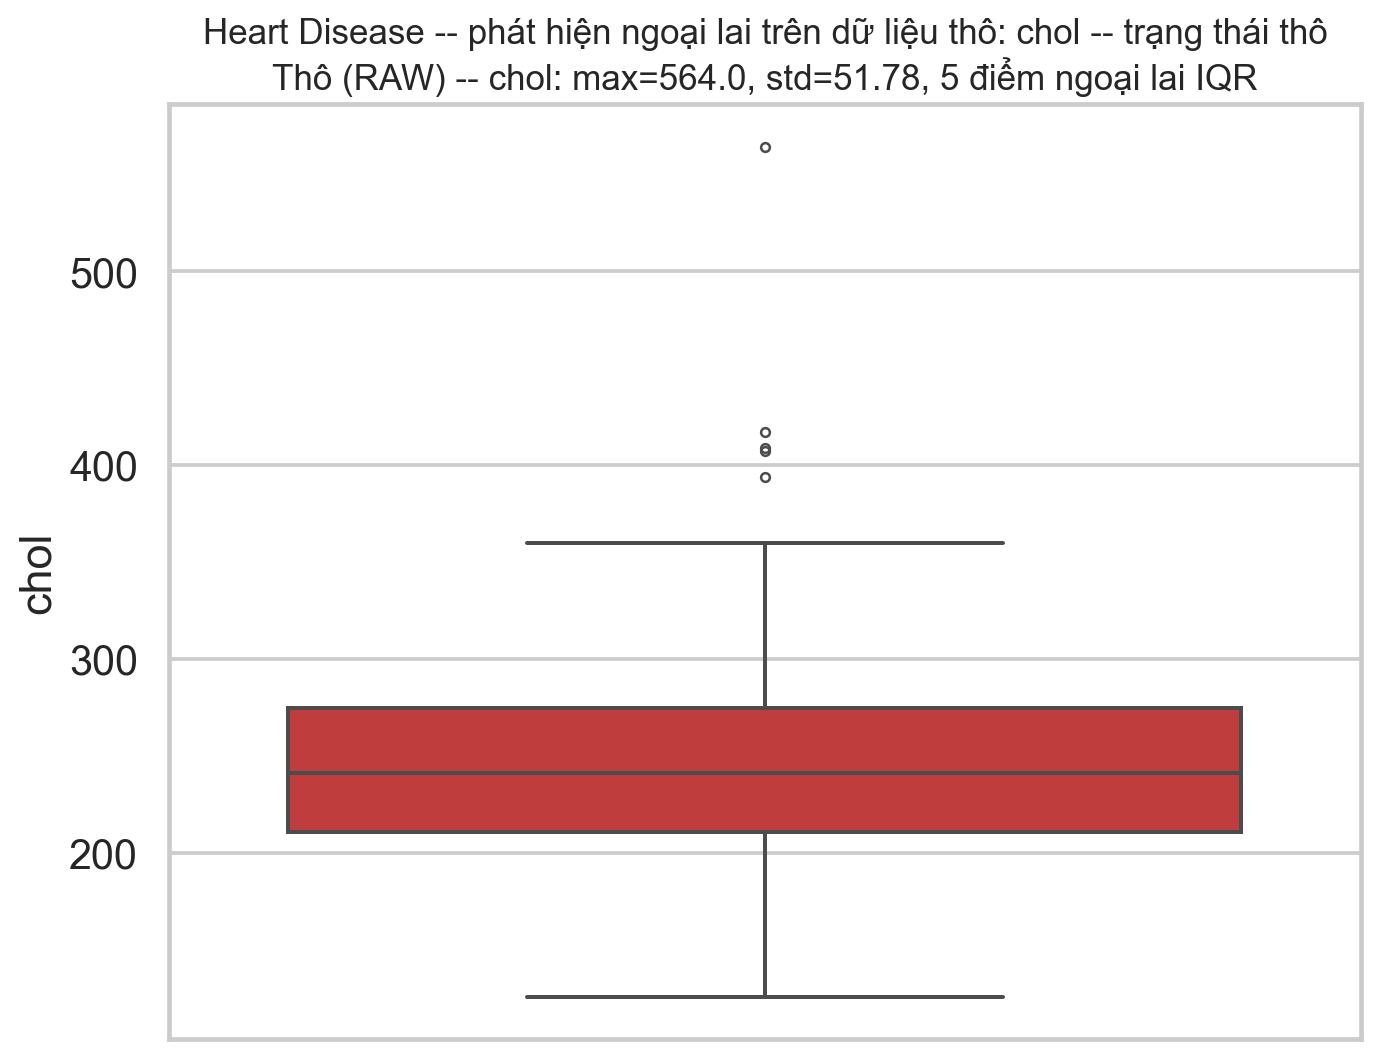
\includegraphics[width=0.72\textwidth]{images/ch3/heart_disease_chol_boxplot_raw.png}
\captionsetup{justification=raggedright,singlelinecheck=false}
\caption[Boxplot \texttt{chol} thô Heart Disease]{Boxplot \texttt{chol} Heart Disease ở \textbf{trạng thái thô}: nhiều điểm ngoại lai ở đuôi phải, giá trị lớn nhất đạt 564 mg/dL (ngưỡng trên hộp $\approx 371$).\\
\footnotesize Python source: \texttt{scripts/generate\_raw\_vs\_cleaned\_boxplots.py}.}
\label{fig:ch4_heart_raw_boxplot}
\end{figure}

\textit{Phát hiện ngoại lai trên dữ liệu thô.} Hình~\ref{fig:ch4_heart_raw_boxplot} cho thấy một số biến định lượng lâm sàng có điểm quan sát nằm ngoài râu hộp theo quy tắc IQR. Nổi bật nhất là \texttt{chol}, với giá trị lớn nhất \textbf{564 mg/dL}, vượt xa ngưỡng trên xấp xỉ $Q3+1.5IQR \approx 371$. Tương tự, \texttt{trestbps} đạt \textbf{200 mmHg} so với ngưỡng xấp xỉ 170, còn \texttt{oldpeak} đạt \textbf{6.2} so với ngưỡng xấp xỉ 4.0. Như vậy, ngoại lai chủ yếu tập trung ở các biến phản ánh cholesterol, huyết áp nghỉ và độ chênh ST khi gắng sức.

\textbf{Làm sạch dữ liệu.} Quy trình tiền xử lý được thực hiện theo ba nguyên tắc sau:

\begin{itemize}[leftmargin=*]
    \item \textbf{Điền khuyết:} \texttt{ca} và \texttt{thal} được điền bằng \textbf{median}. Cách chọn này phù hợp với các biến được mã hóa theo mức hoặc có phân phối lệch, vì median ít nhạy với giá trị cực trị hơn mean.
    \item \textbf{Xử lý ngoại lai:} \emph{clipping theo quy tắc IQR} trên các biến định lượng \texttt{age}, \texttt{trestbps}, \texttt{chol}, \texttt{thalach}, \texttt{oldpeak}, \texttt{ca} -- mọi giá trị ngoài $[Q1-1.5IQR,\; Q3+1.5IQR]$ được kéo về biên hộp (ví dụ \texttt{chol}=564 $\to$ 371, \texttt{trestbps}=200 $\to$ 170).
    \item \textbf{Chuẩn hóa:} \emph{chưa áp dụng} ở giai đoạn thống kê mô tả để giữ nguyên đơn vị lâm sàng gốc; Min--Max Scaling hoặc Z-score chỉ được dùng ở chương học máy khi thuật toán yêu cầu thang đo đồng nhất.
\end{itemize}

\begin{figure}[H]
\centering
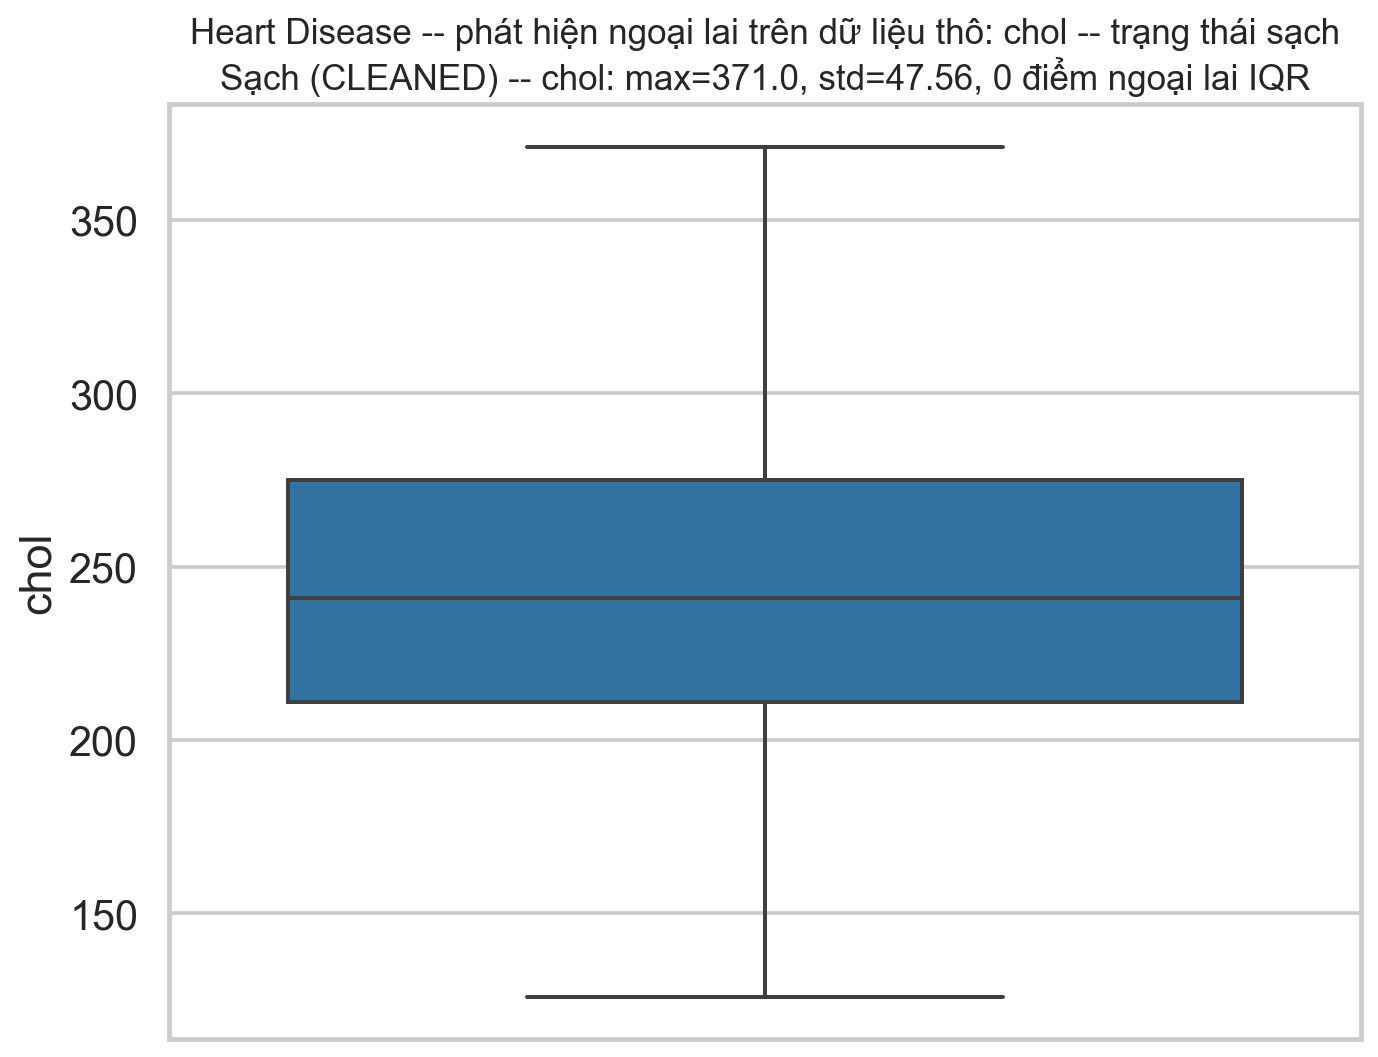
\includegraphics[width=0.72\textwidth]{images/ch3/heart_disease_chol_boxplot_cleaned.png}
\captionsetup{justification=raggedright,singlelinecheck=false}
\caption[Boxplot \texttt{chol} sạch Heart Disease]{Boxplot \texttt{chol} Heart Disease ở \textbf{trạng thái sạch}: sau clipping IQR, các điểm ngoại lai đuôi phải được nén về ngưỡng trên hộp, max giảm từ 564 xuống $\approx 371$.\\
\footnotesize Python source: \texttt{scripts/generate\_raw\_vs\_cleaned\_boxplots.py}.}
\label{fig:ch4_heart_cleaned_boxplot}
\end{figure}

\textbf{Bước 1. Phân loại bản chất biến.} Trước khi lựa chọn thống kê và biểu đồ, các biến được phân loại theo bản chất đo lường. Cách phân loại này giúp tránh áp dụng sai chỉ số, chẳng hạn không dùng mean/median để diễn giải biến định danh như \texttt{cp}.

\vspace{1\baselineskip}

\begin{table}[H]
\centering
\caption{Phân loại biến tiêu biểu trong Heart Disease}
\label{tab:ch4_heart_variable_types}
\small
\begin{tabularx}{\textwidth}{p{0.18\textwidth}p{0.27\textwidth}p{0.25\textwidth}Y}
\toprule
Biến & Bản chất & Thống kê dùng & Biểu đồ phù hợp \\
\midrule
\texttt{age} & Quantitative Discrete & Mean, median, SD, IQR & Histogram, boxplot \\
\texttt{cp} & Qualitative (nominal) & Tần suất, tần suất tương đối, mode & Bar chart, pie chart \\
\texttt{trestbps} & Quantitative Continuous & Range, SD, IQR & Histogram, boxplot \\
\texttt{chol} & Quantitative Continuous & Dữ liệu bất thường theo IQR & Boxplot thô--sạch \\
\texttt{thalach} & Quantitative Continuous & Tương quan với tuổi/target & Scatter plot \\
\texttt{oldpeak} & Quantitative Continuous & Độ lệch phải, CV & Histogram, boxplot \\
\bottomrule
\end{tabularx}
\end{table}

\textbf{Bước 2. Bảng tần suất và thống kê mô tả.} Với biến Qualitative, báo cáo sử dụng tần suất tuyệt đối, tần suất tương đối và mode. Với biến Quantitative, báo cáo sử dụng các số đo xu hướng trung tâm và độ phân tán như mean, median, standard deviation, range và IQR.

\begin{table}[H]
\centering
\caption[Bảng tần suất biến \texttt{cp} trong Heart Disease]{Bước 2 -- Bảng tần suất biến \texttt{cp} trong Heart Disease. Source: \texttt{outputs/tables/heart\_disease\_frequency\_cp.csv}.}
\label{tab:ch4_cp_frequency}
\small
\begin{tabular}{lrr}
\toprule
Loại đau ngực \texttt{cp} & Tần suất tuyệt đối & Tần suất tương đối \\
\midrule
4.0 (không triệu chứng) & 144 & 47.52\% \\
3.0 (đau không điển hình) & 86 & 28.38\% \\
2.0 (đau điển hình) & 50 & 16.50\% \\
1.0 (đau thắt ngực điển hình) & 23 & 7.59\% \\
\bottomrule
\end{tabular}
\end{table}

Bảng \ref{tab:ch4_cp_frequency} cho thấy mode của \texttt{cp} là lớp 4.0; gần một nửa bệnh nhân thuộc nhóm đau ngực không triệu chứng. Kết quả này có ý nghĩa lâm sàng đáng chú ý: nếu chỉ dựa vào triệu chứng đau ngực điển hình, nguy cơ bệnh tim có thể bị đánh giá thấp. Do đó, \texttt{cp} cần được diễn giải đồng thời với \texttt{thalach}, \texttt{oldpeak}, \texttt{trestbps} và các biến lâm sàng khác.

\begin{table}[H]
\centering
\caption[Phân phối tần suất các biến Qualitative Heart Disease]{Phân phối tần suất (Frequency Distribution) các biến Qualitative tiêu biểu trong Heart Disease: tần suất tuyệt đối, tần suất tương đối và Mode. Source: \texttt{outputs/tables/heart\_disease\_frequency\_*.csv}.}
\label{tab:ch4_heart_qualitative_freq}
\scriptsize
\setlength{\tabcolsep}{4pt}
\begin{tabular}{llrrr}
\toprule
Biến & Lớp & Tần suất tuyệt đối & Tần suất tương đối & Mode \\
\midrule
\texttt{sex} & 1 (nam) & 206 & 67.99\% & \multirow{4}{*}{1 (nam)} \\
 & 0 (nữ) & 97 & 32.01\% & \\
\texttt{fbs} & 0 ($\leq$ 120 mg/dl) & 258 & 85.15\% & \multirow{4}{*}{0} \\
 & 1 ($>$ 120 mg/dl) & 45 & 14.85\% & \\
\texttt{restecg} & 0 (bình thường) & 151 & 49.83\% & \multirow{6}{*}{0} \\
 & 2 (LV hypertrophy) & 148 & 48.84\% & \\
 & 1 (ST-T bất thường) & 4 & 1.32\% & \\
\texttt{exang} & 0 (không) & 204 & 67.33\% & \multirow{4}{*}{0} \\
 & 1 (có) & 99 & 32.67\% & \\
\bottomrule
\end{tabular}
\end{table}

\textbf{Nhận xét.} Đối với biến Qualitative, mean và median không phản ánh ý nghĩa thống kê phù hợp; vì vậy bảng phân phối tần suất và mode là công cụ mô tả chính. Bảng \ref{tab:ch4_heart_qualitative_freq} cho thấy mẫu Heart Disease mất cân bằng giới, với 67.99\% quan sát là nam (mode = 1). Phần lớn bệnh nhân không có đường huyết lúc đói cao (\texttt{fbs} mode = 0, 85.15\%) và không bị đau thắt ngực khi gắng sức (\texttt{exang} mode = 0, 67.33\%). Đáng chú ý, \texttt{restecg} phân bố gần như song song giữa lớp 0 (49.83\%) và lớp 2 (48.84\%), trong khi lớp 1 chỉ chiếm 1.32\%; đặc điểm này cần được lưu ý khi mã hóa one-hot cho mô hình học máy.

\begin{table}[H]
\centering
\caption[Thống kê thô/sạch Heart Disease]{So sánh thống kê mô tả Heart Disease ở hai trạng thái: \textbf{thô} (chưa làm sạch) và \textbf{sạch} (sau điền median + clipping IQR). Các cột in đậm là chỉ số thay đổi nhiều nhất. Source: \texttt{outputs/tables/heart\_disease\_summary.csv}.}
\label{tab:ch4_heart_stats_raw_clean}
\footnotesize
\setlength{\tabcolsep}{4pt}
\begin{tabular}{lcrrrrrr}
\toprule
Biến & Trạng thái & Mean & Median & \textbf{Std} & \textbf{Max} & \textbf{Range} & IQR \\
\midrule
\texttt{age} & thô & 54.44 & 56.00 & 9.04 & 77.00 & 48.00 & 13.00 \\
 & sạch & 54.44 & 56.00 & 9.04 & 77.00 & 48.00 & 13.00 \\
\midrule
\texttt{trestbps} & thô & 131.69 & 130.00 & \textbf{17.60} & \textbf{200.00} & \textbf{106.00} & 20.00 \\
 & sạch & 131.35 & 130.00 & \textbf{16.65} & \textbf{170.00} & \textbf{76.00} & 20.00 \\
\midrule
\texttt{chol} & thô & 246.69 & 241.00 & \textbf{51.78} & \textbf{564.00} & \textbf{438.00} & 64.00 \\
 & sạch & 245.58 & 241.00 & \textbf{47.56} & \textbf{371.00} & \textbf{245.00} & 64.00 \\
\midrule
\texttt{thalach} & thô & 149.61 & 153.00 & 22.88 & 202.00 & 131.00 & 32.50 \\
 & sạch & 149.65 & 153.00 & 22.73 & 202.00 & 117.25 & 32.50 \\
\midrule
\texttt{oldpeak} & thô & 1.04 & 0.80 & 1.16 & 6.20 & 6.20 & 1.60 \\
 & sạch & 1.02 & 0.80 & 1.11 & 4.00 & 4.00 & 1.60 \\
\bottomrule
\end{tabular}
\end{table}

\textit{Nhận xét thô/sạch.} Các biến ít chịu ảnh hưởng của ngoại lai như \texttt{age} và \texttt{thalach} gần như không thay đổi sau tiền xử lý. Ngược lại, \texttt{chol} giảm standard deviation từ 51.78 xuống 47.56, giá trị lớn nhất từ 564 xuống 371 và range từ 438 xuống 245; \texttt{trestbps} cũng giảm giá trị lớn nhất từ 200 xuống 170. Mean và median gần như ổn định, cho thấy clipping chủ yếu kiểm soát phần đuôi cực trị mà không làm thay đổi cấu trúc trung tâm của phân phối.

\textbf{Nhận xét về hình dáng phân phối.} Quan hệ giữa mean, median và mode cho phép nhận diện sơ bộ hướng lệch của phân phối. Trong Heart Disease, \texttt{age} có mean 54.44 \textless{} median 56 \textless{} mode 58, cho thấy phân phối \emph{lệch trái nhẹ}; mẫu dữ liệu tập trung nhiều ở nhóm trung niên và cao tuổi. Ngược lại, \texttt{chol} và \texttt{oldpeak} đều có mean lớn hơn median (\texttt{oldpeak}: 1.02 so với 0.80, mode = 0), phản ánh phân phối \emph{lệch phải}. Riêng \texttt{oldpeak} lệch phải rõ vì nhiều bệnh nhân có ST depression bằng 0, làm mode nằm ở biên thấp của thang đo.

\texttt{thalach} có mean 149.65 \textless{} median 153 \textless{} mode 162, cũng gợi ý phân phối lệch trái, phù hợp với hiện tượng một số bệnh nhân lớn tuổi hoặc có hạn chế gắng sức đạt nhịp tim tối đa thấp. Về độ phân tán, CV của \texttt{oldpeak} đạt 1.084, cao hơn rõ rệt so với \texttt{age}, \texttt{trestbps} và \texttt{thalach} (0.13--0.17). IQR của \texttt{chol} bằng 64 và là một trong các khoảng tứ phân vị lớn nhất trong nhóm biến lâm sàng, vì vậy boxplot là biểu đồ cần thiết để nhận diện các ca cholesterol cực trị. Nhìn chung, các biến liên tục có IQR tương đối hẹp nhưng range rộng (ví dụ \texttt{chol}: IQR 64 so với range 245), cho thấy phần lớn quan sát tập trung quanh vùng trung tâm nhưng vẫn tồn tại đuôi phân phối dài, một đặc điểm thường gặp trong dữ liệu y tế thực tế.

\textbf{Bước 3. Trực quan hóa dữ liệu.} Hệ thống biểu đồ được lựa chọn theo bản chất biến: bar chart cho biến định tính, histogram và boxplot cho biến định lượng một chiều, scatter plot cho quan hệ hai biến, biểu đồ phân bố target để kiểm tra cân bằng lớp và heatmap để khảo sát tương quan tuyến tính giữa các biến định lượng.

\begin{figure}[H]
\centering
\begin{subfigure}{0.92\textwidth}
 \centering
 \includegraphics[width=\textwidth]{images/ch3/heart_disease_chest_pain_bar.png}
 \caption{Python -- Bar chart \texttt{cp}}
\end{subfigure}

\par\medskip

\begin{subfigure}{0.92\textwidth}
 \centering
 \includegraphics[width=\textwidth]{images/ch3/excel_heart_cp_bar_preview.png}
 \caption{Excel -- Column chart \texttt{cp}}
\end{subfigure}
\captionsetup{justification=raggedright,singlelinecheck=false}
\caption[Bar chart tần suất \texttt{cp}: Python và Excel]{Tần suất loại đau ngực Heart Disease vẽ bằng Python và Excel.\\
\footnotesize Python source: \texttt{src/analyze\_heart\_disease.py}.\\
Excel source/workbook: \texttt{src/create\_excel\_visualizations.py}, \texttt{excel/excel\_visualization\_comparison\_native.xlsx}, sheet \texttt{Heart Frequency}.}
\label{fig:ch4_cp_bar}
\end{figure}

\textbf{Nhận xét Hình \ref{fig:ch4_cp_bar}.} Hai phiên bản Python và Excel cho cùng một thông điệp: \texttt{cp=4} là nhóm có tần suất cao nhất, vượt rõ các nhóm còn lại. Vì \texttt{cp} là biến Qualitative nominal, biểu đồ cột là lựa chọn phù hợp hơn histogram; kết quả này cũng xác nhận mode trong Bảng \ref{tab:ch4_cp_frequency}.

\begin{figure}[H]
\centering
\begin{subfigure}{0.92\textwidth}
 \centering
 \includegraphics[width=\textwidth]{images/ch3/heart_disease_age_raw_vs_cleaned.png}
 \caption{Python -- Histogram tuổi thô/sạch}
\end{subfigure}

\par\medskip

\begin{subfigure}{0.92\textwidth}
 \centering
 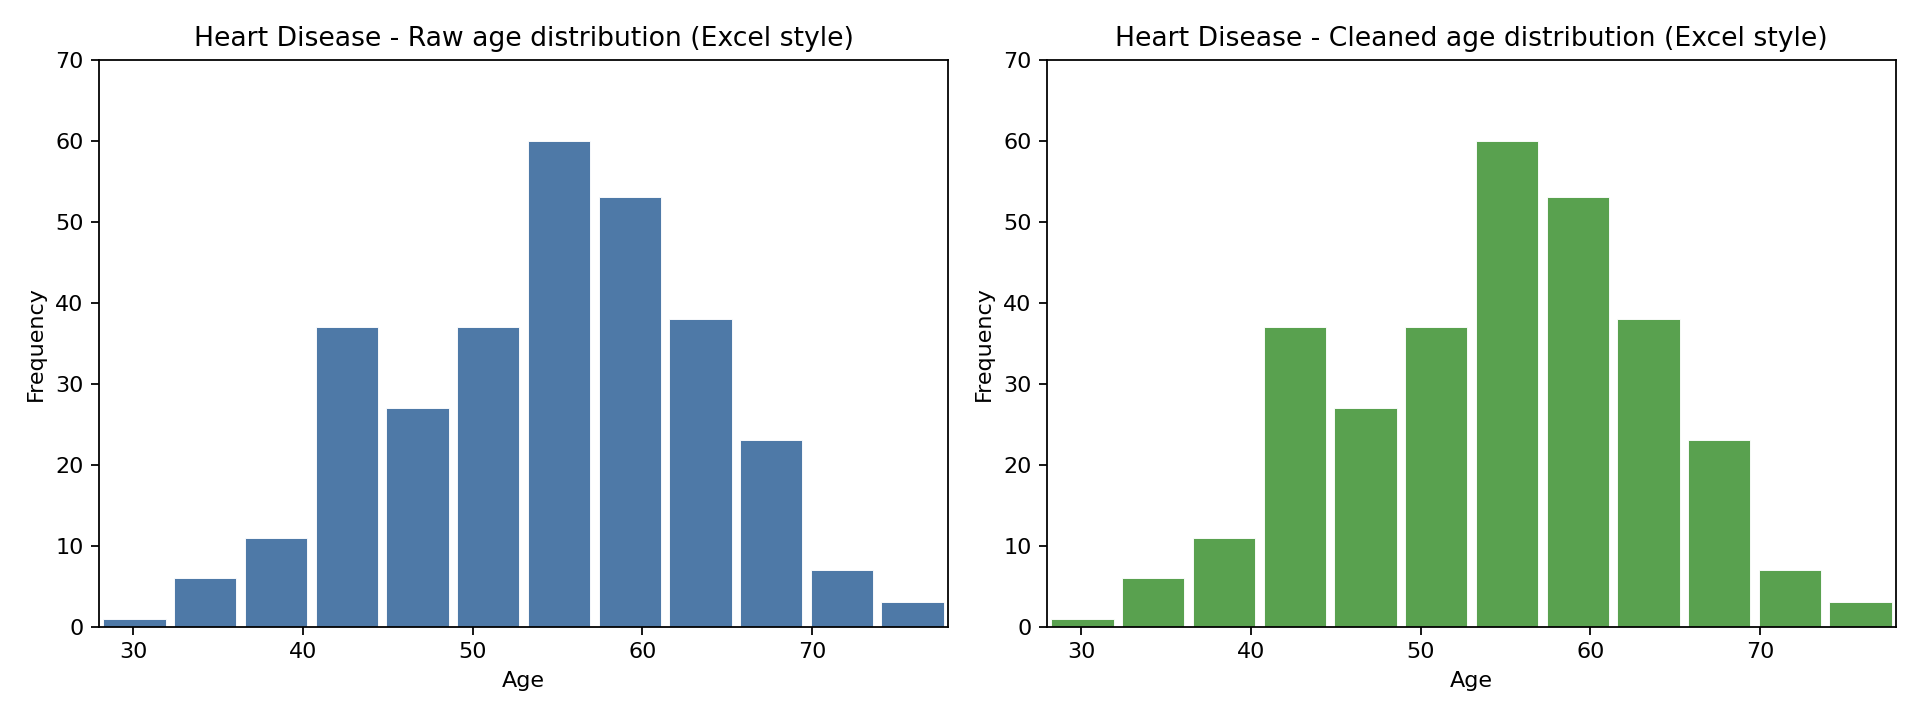
\includegraphics[width=\textwidth]{images/ch3/excel_heart_age_raw_vs_cleaned_preview.png}
 \caption{Excel -- Histogram tuổi thô/sạch}
\end{subfigure}
\captionsetup{justification=raggedright,singlelinecheck=false}
\caption[Histogram tuổi Heart Disease: Python và Excel]{Histogram tuổi thô/sạch trên Heart Disease, đối chiếu giữa Python và Excel.\\
\footnotesize Python source: \texttt{src/analyze\_heart\_disease.py}.\\
Excel source/workbook: \texttt{src/create\_excel\_visualizations.py}, \texttt{excel/excel\_visualization\_comparison\_native.xlsx}, sheet \texttt{Heart Age Hist}.}
\label{fig:ch4_heart_hist}
\end{figure}

\textbf{Nhận xét Hình \ref{fig:ch4_heart_hist}.} Histogram tuổi thô và histogram tuổi sau tiền xử lý gần như trùng nhau, cho thấy biến \texttt{age} không chịu tác động đáng kể từ bước làm sạch. Phân phối tập trung ở nhóm trung niên và cao tuổi, trong đó khoảng 50--60 tuổi xuất hiện dày hơn các nhóm còn lại; kết quả này phù hợp với bối cảnh bệnh tim thường được khảo sát nhiều ở nhóm tuổi có nguy cơ cao.

\begin{figure}[H]
\centering
\includegraphics[width=0.92\textwidth]{images/ch3/heart_disease_cholesterol_boxplot.png}
\captionsetup{justification=raggedright,singlelinecheck=false}
\caption[Boxplot cholesterol Heart Disease]{Boxplot cholesterol trên Heart Disease.\\
\footnotesize Python source: \texttt{src/analyze\_heart\_disease.py}.}
\label{fig:ch4_heart_boxplot}
\end{figure}

\textbf{Nhận xét Hình \ref{fig:ch4_heart_boxplot}.} Boxplot cholesterol theo \texttt{target\_binary} cho thấy cả hai nhóm đều có giá trị nằm ngoài râu IQR, đặc biệt ở vùng cholesterol cao. Trung vị giữa nhóm có bệnh và không bệnh không tách biệt mạnh, vì vậy \texttt{chol} riêng lẻ chưa đủ để phân loại bệnh tim; tuy nhiên, độ trải rộng và các giá trị cực trị vẫn là thông tin lâm sàng cần được kiểm soát trong tiền xử lý.

\textit{Đối chiếu thô/sạch.} Ba biểu đồ tiếp theo đặt dữ liệu thô (đỏ) cạnh dữ liệu sạch (xanh), qua đó thể hiện trực quan tác động của điền khuyết và clipping theo IQR.

\begin{figure}[H]
\centering
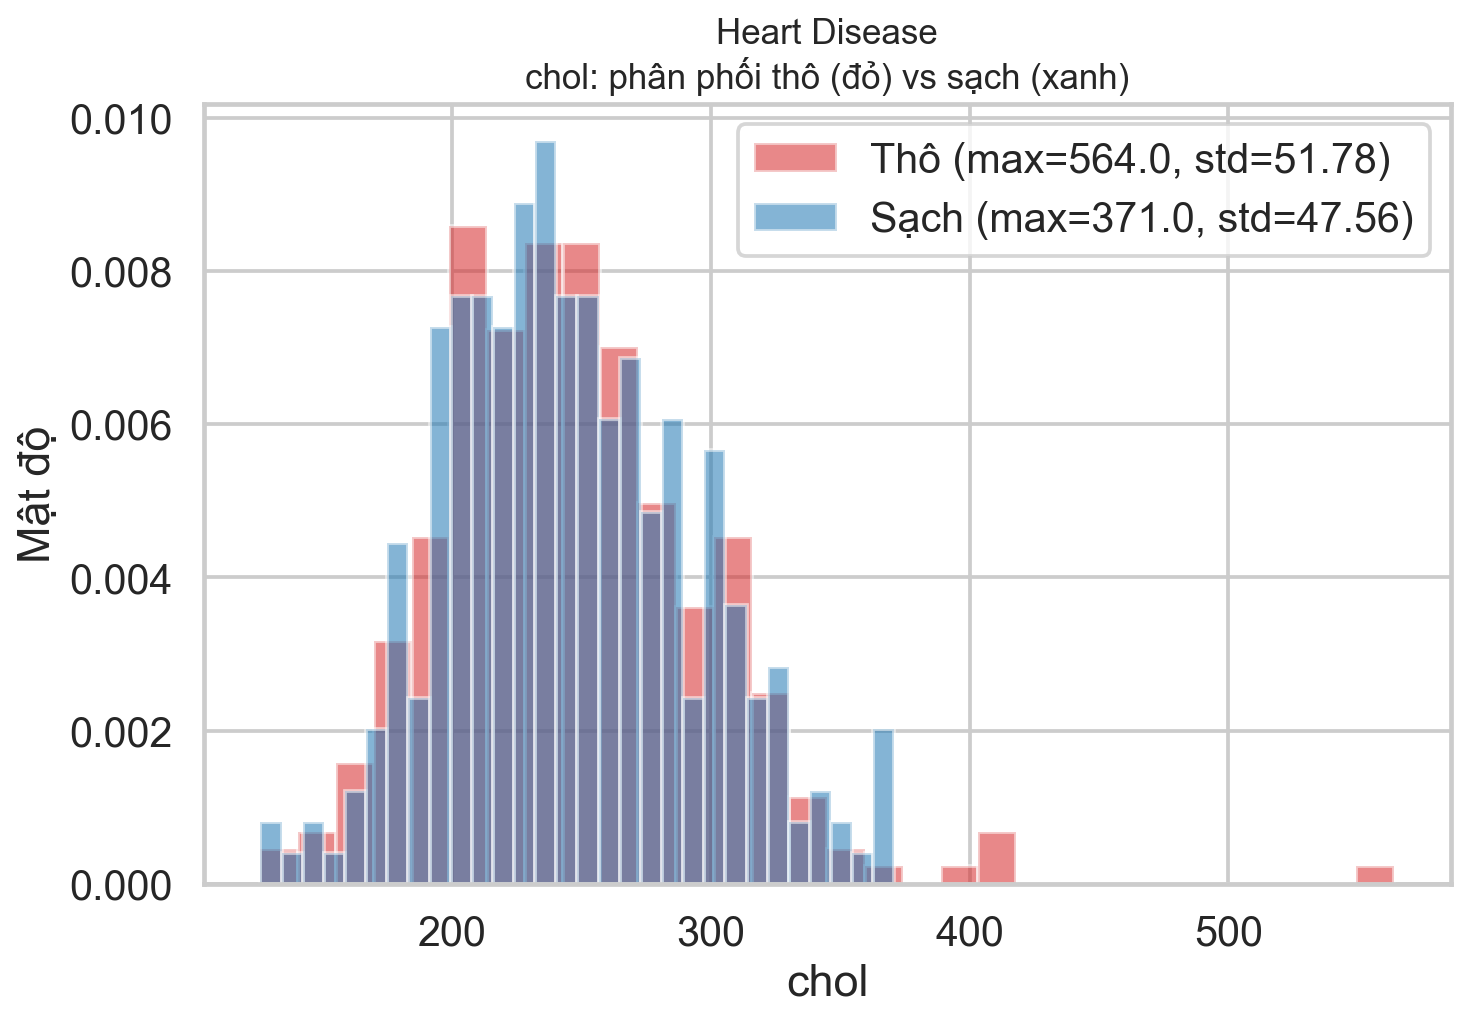
\includegraphics[width=0.82\textwidth]{images/ch3/heart_disease_chol_hist_raw_vs_cleaned.png}
\captionsetup{justification=raggedright,singlelinecheck=false}
\caption[Histogram \texttt{chol} thô/sạch Heart Disease]{Histogram \texttt{chol} Heart Disease: dữ liệu thô (đỏ, đuôi phải đến 564) chồng lên dữ liệu sạch (xanh, đuôi được nén về 371).\\
\footnotesize Python source: \texttt{scripts/generate\_raw\_vs\_cleaned\_boxplots.py}.}
\label{fig:ch4_heart_chol_hist_compare}
\end{figure}

\begin{figure}[H]
\centering
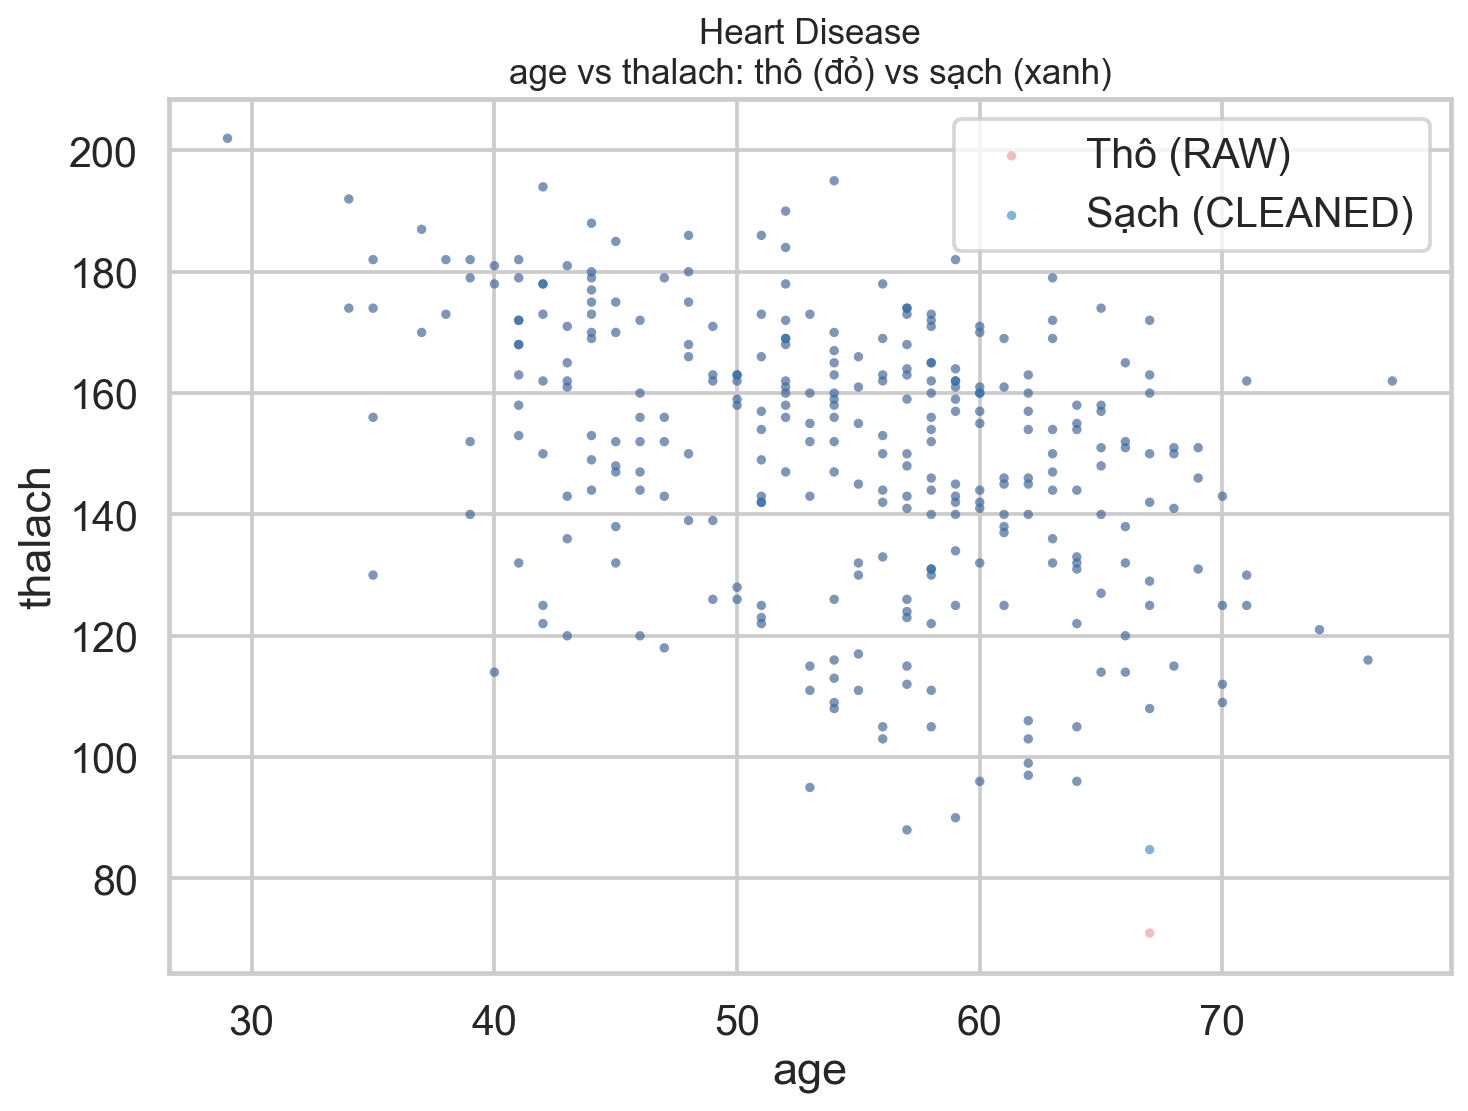
\includegraphics[width=0.82\textwidth]{images/ch3/heart_disease_age_thalach_scatter_raw_vs_cleaned.png}
\captionsetup{justification=raggedright,singlelinecheck=false}
\caption[Scatter \texttt{age}--\texttt{thalach} thô/sạch Heart Disease]{Scatter \texttt{age}--\texttt{thalach} Heart Disease: dữ liệu thô (đỏ, mờ) gần như trùng dữ liệu sạch (xanh) vì cả hai biến ít ngoại lai.\\
\footnotesize Python source: \texttt{scripts/generate\_raw\_vs\_cleaned\_boxplots.py}.}
\label{fig:ch4_heart_scatter_compare}
\end{figure}

\begin{figure}[H]
\centering
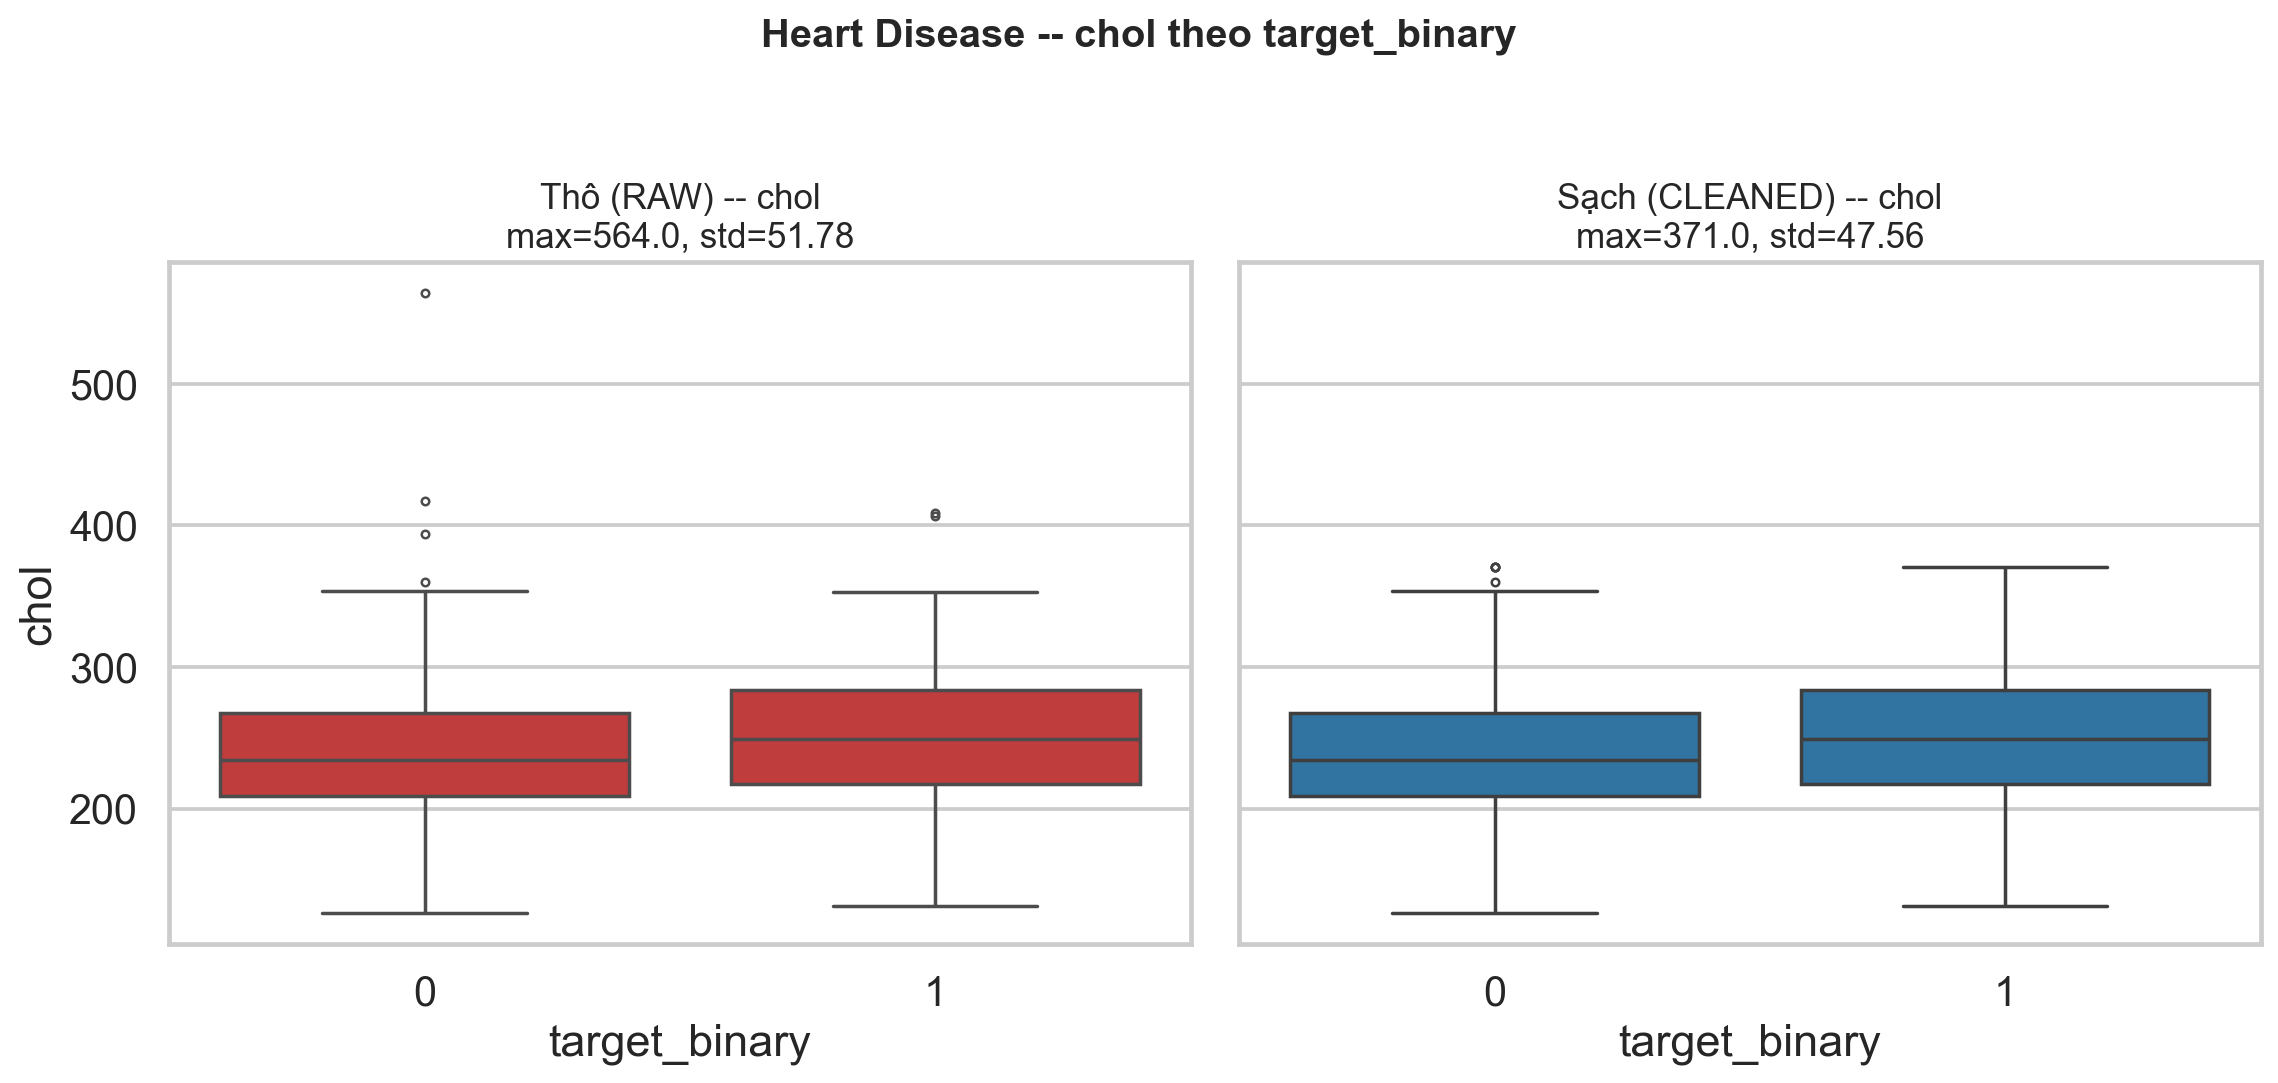
\includegraphics[width=0.95\textwidth]{images/ch3/heart_disease_chol_boxplot_by_target_raw_vs_cleaned.png}
\captionsetup{justification=raggedright,singlelinecheck=false}
\caption[Boxplot \texttt{chol} theo target thô/sạch Heart Disease]{Boxplot \texttt{chol} theo \texttt{target\_binary}: thô (trái) có nhiều điểm ngoại lai ở cả hai lớp; sạch (phải) sau clipping giảm ngoại lai nhưng vẫn giữ trung vị tách hai nhóm.\\
\footnotesize Python source: \texttt{scripts/generate\_raw\_vs\_cleaned\_boxplots.py}.}
\label{fig:ch4_heart_boxplot_by_target_compare}
\end{figure}

\textbf{Nhận xét.} Histogram \texttt{chol} (Hình~\ref{fig:ch4_heart_chol_hist_compare}) cho thấy đuôi phải của dữ liệu thô kéo dài tới 564, trong khi dữ liệu sạch dừng ở 371. Phần chồng lấn lớn giữa hai phân phối xác nhận rằng clipping chủ yếu nén vùng đuôi, không làm thay đổi phần lõi của dữ liệu. Scatter \texttt{age}--\texttt{thalach} (Hình~\ref{fig:ch4_heart_scatter_compare}) gần như trùng nhau vì hai biến này ít chịu ảnh hưởng của ngoại lai. Boxplot theo target (Hình~\ref{fig:ch4_heart_boxplot_by_target_compare}) cho thấy sau clipping, số điểm ngoài râu giảm rõ nhưng trung vị giữa hai lớp bệnh/không bệnh vẫn được duy trì, nghĩa là tín hiệu phân loại cơ bản không bị triệt tiêu.

\begin{figure}[H]
\centering
\begin{subfigure}{0.92\textwidth}
 \centering
 \includegraphics[width=\textwidth]{images/ch3/heart_disease_age_thalach_scatter.png}
 \caption{Python -- \texttt{age} và \texttt{thalach}}
\end{subfigure}

\par\medskip

\begin{subfigure}{0.92\textwidth}
 \centering
 \includegraphics[width=\textwidth]{images/ch3/excel_heart_age_thalach_scatter_preview.png}
 \caption{Excel -- \texttt{age} và \texttt{thalach}}
\end{subfigure}
\captionsetup{justification=raggedright,singlelinecheck=false}
\caption[Scatter plot \texttt{age}--\texttt{thalach}: Python và Excel]{Scatter plot giữa tuổi và nhịp tim tối đa.\\
\footnotesize Python source: \texttt{src/analyze\_heart\_disease.py}.\\
Excel source/workbook: \texttt{src/create\_excel\_visualizations.py}, \texttt{excel/excel\_visualization\_comparison\_native.xlsx}, sheet \texttt{Heart Scatter}.}
\label{fig:ch4_heart_scatter}
\end{figure}

\textbf{Nhận xét Hình \ref{fig:ch4_heart_scatter}.} Scatter plot cho thấy xu hướng quan hệ âm giữa \texttt{age} và \texttt{thalach}: bệnh nhân lớn tuổi thường đạt nhịp tim tối đa thấp hơn trong kiểm tra gắng sức. Xu hướng này phù hợp về mặt sinh lý, nhưng cần được diễn giải như mối liên hệ thống kê quan sát được, không phải quan hệ nhân quả trực tiếp.

\begin{figure}[H]
\centering
\begin{subfigure}{0.92\textwidth}
 \centering
 \includegraphics[width=\textwidth]{images/ch3/heart_disease_target_distribution.png}
 \caption{Python -- Phân bố target}
\end{subfigure}

\par\medskip

\begin{subfigure}{0.92\textwidth}
 \centering
 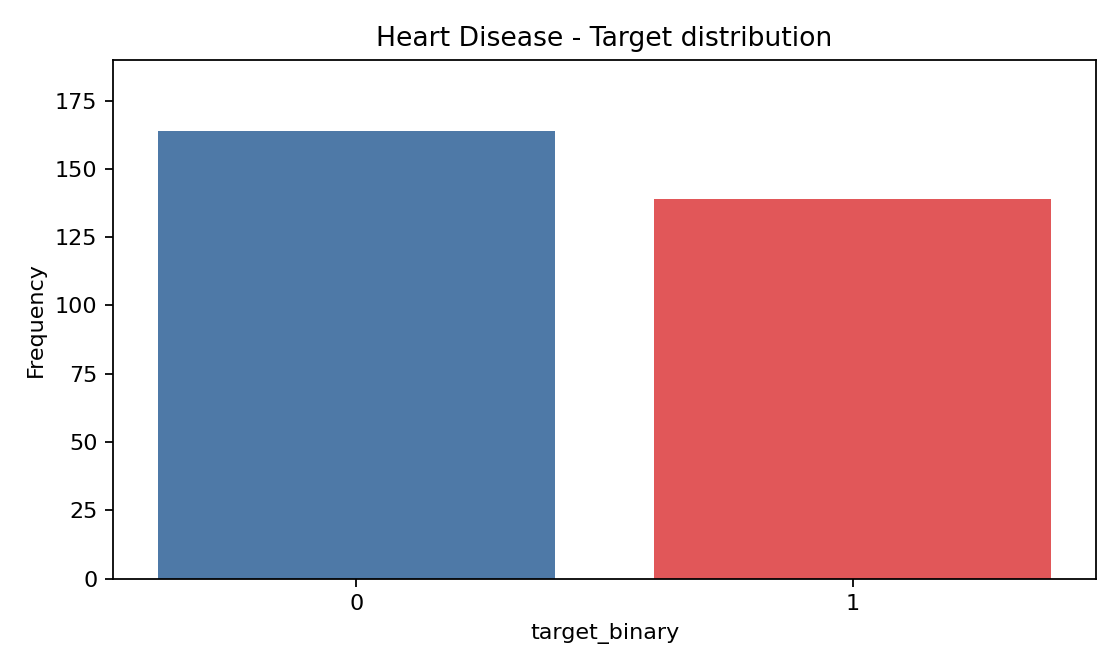
\includegraphics[width=\textwidth]{images/ch3/excel_heart_target_distribution_preview.png}
 \caption{Excel -- Phân bố target}
\end{subfigure}
\captionsetup{justification=raggedright,singlelinecheck=false}
\caption[Phân bố target Heart Disease: Python và Excel]{Phân bố target Heart Disease, đối chiếu giữa Python và Excel.\\
\footnotesize Python source: \texttt{src/analyze\_heart\_disease.py}.\\
Excel source/workbook: \texttt{src/create\_excel\_visualizations.py}, \texttt{excel/excel\_visualization\_comparison\_native.xlsx}, sheet \texttt{Heart Target}.}
\label{fig:ch4_heart_target}
\end{figure}

\textbf{Nhận xét Hình \ref{fig:ch4_heart_target}.} Phân bố target cho thấy hai lớp bệnh/không bệnh tương đối cân bằng. Vì vậy, accuracy có thể được dùng như chỉ báo ban đầu, nhưng vẫn cần đọc đồng thời precision, recall và F1 để tránh bỏ sót sai số ở từng lớp.

\begin{figure}[H]
\centering
\includegraphics[width=0.86\textwidth]{images/ch3/heart_disease_correlation_heatmap.png}
\captionsetup{justification=raggedright,singlelinecheck=false}
\caption[Heatmap tương quan Heart Disease]{Heatmap tương quan các biến định lượng Heart Disease.\\
\footnotesize Python source: \texttt{src/analyze\_heart\_disease.py}.}
\label{fig:ch4_heart_corr}
\end{figure}

\textbf{Nhận xét Hình \ref{fig:ch4_heart_corr}.} Heatmap tương quan cho thấy \texttt{thalach} có tương quan âm với \texttt{target\_binary}, trong khi \texttt{oldpeak} có tương quan dương. Hai biến này phản ánh hai khía cạnh khác nhau của đáp ứng tim mạch khi gắng sức: khả năng đạt nhịp tim tối đa và mức bất thường ST. Do đó, chúng cung cấp tín hiệu bổ sung cho bài toán phân loại, dù heatmap chỉ phản ánh tương quan tuyến tính và không thay thế được đánh giá mô hình đa biến.

\textbf{Bước 4. So sánh trước--sau tiền xử lý.} Bảng~\ref{tab:ch4_heart_preprocess} đặt các chỉ số của trạng thái thô cạnh trạng thái sạch; các hình thô/sạch ở trên minh họa trực tiếp tác động của điền khuyết và clipping IQR.

\begin{table}[H]
\centering
\caption[So sánh dữ liệu thô và dữ liệu sạch Heart Disease]{Bước 4 -- So sánh dữ liệu thô và dữ liệu sạch Heart Disease (điền median cho \texttt{ca}/\texttt{thal}, clipping IQR cho biến định lượng). Source: \texttt{outputs/tables/heart\_disease\_preprocessing\_comparison.csv}.}
\label{tab:ch4_heart_preprocess}
\small
\begin{tabular}{lrrrrrr}
\toprule
Biến & Max thô & Max sạch & Std thô & Std sạch & Range thô & Range sạch \\
\midrule
\texttt{age} & 77.00 & 77.00 & 9.04 & 9.04 & 48.00 & 48.00 \\
\texttt{trestbps} & 200.00 & 170.00 & 17.60 & 16.65 & 106.00 & 76.00 \\
\texttt{chol} & 564.00 & 371.00 & 51.78 & 47.56 & 438.00 & 245.00 \\
\texttt{thalach} & 202.00 & 202.00 & 22.88 & 22.73 & 131.00 & 117.25 \\
\texttt{oldpeak} & 6.20 & 4.00 & 1.16 & 1.11 & 6.20 & 4.00 \\
\bottomrule
\end{tabular}
\end{table}

Bảng \ref{tab:ch4_heart_preprocess} cho thấy hiệu quả của xử lý ngoại lai theo IQR: \texttt{chol} giảm giá trị lớn nhất từ 564 xuống 371 và range giảm gần một nửa; \texttt{trestbps} cũng giảm giá trị lớn nhất từ 200 xuống 170. Các điểm nằm ngoài râu boxplot ở Hình \ref{fig:ch4_heart_boxplot} là nhóm quan sát cần được đánh dấu trước khi clipping. Sau xử lý, độ lệch chuẩn của \texttt{chol} giảm từ 51.78 xuống 47.56 và \texttt{trestbps} giảm từ 17.60 xuống 16.65; trong khi đó, các chỉ số trung tâm không thay đổi đáng kể. Điều này cho thấy tiền xử lý làm giảm ảnh hưởng của giá trị cực trị nhưng vẫn bảo toàn cấu trúc chính của dữ liệu.

\textbf{Kết luận cho Heart Disease.} Có ba kết quả chính rút ra từ phân tích trước--sau tiền xử lý. Thứ nhất, toàn bộ ô khuyết được xử lý sau khi điền median cho \texttt{ca} và \texttt{thal}. Thứ hai, độ phân tán của các biến có ngoại lai giảm có kiểm soát; riêng \texttt{chol} giảm standard deviation 8.1\% (51.78$\to$47.56) và range giảm 44\% (438$\to$245). Thứ ba, các biến vốn ổn định như \texttt{age} gần như không thay đổi, thể hiện qua histogram thô/sạch gần trùng nhau. Như vậy, quy trình tiền xử lý làm giảm ảnh hưởng của giá trị cực trị và ô khuyết, đồng thời vẫn giữ được xu hướng trung tâm và tín hiệu phân biệt chính của bộ dữ liệu.

\subsubsection{CDC Diabetes Health Indicators}

CDC Diabetes có 253\,680 mẫu và 21 biến giải thích, là bộ dữ liệu lớn nhất của nhóm A.

\textbf{Trạng thái dữ liệu thô (chưa làm sạch).} Ở trạng thái thô, CDC Diabetes \emph{không có ô khuyết thiếu} (0/253\,680 dòng, theo \texttt{outputs/tables/cdc\_diabetes\_missing\_values.csv}); do đó bước điền khuyết không cần thiết.

\begin{figure}[H]
\centering
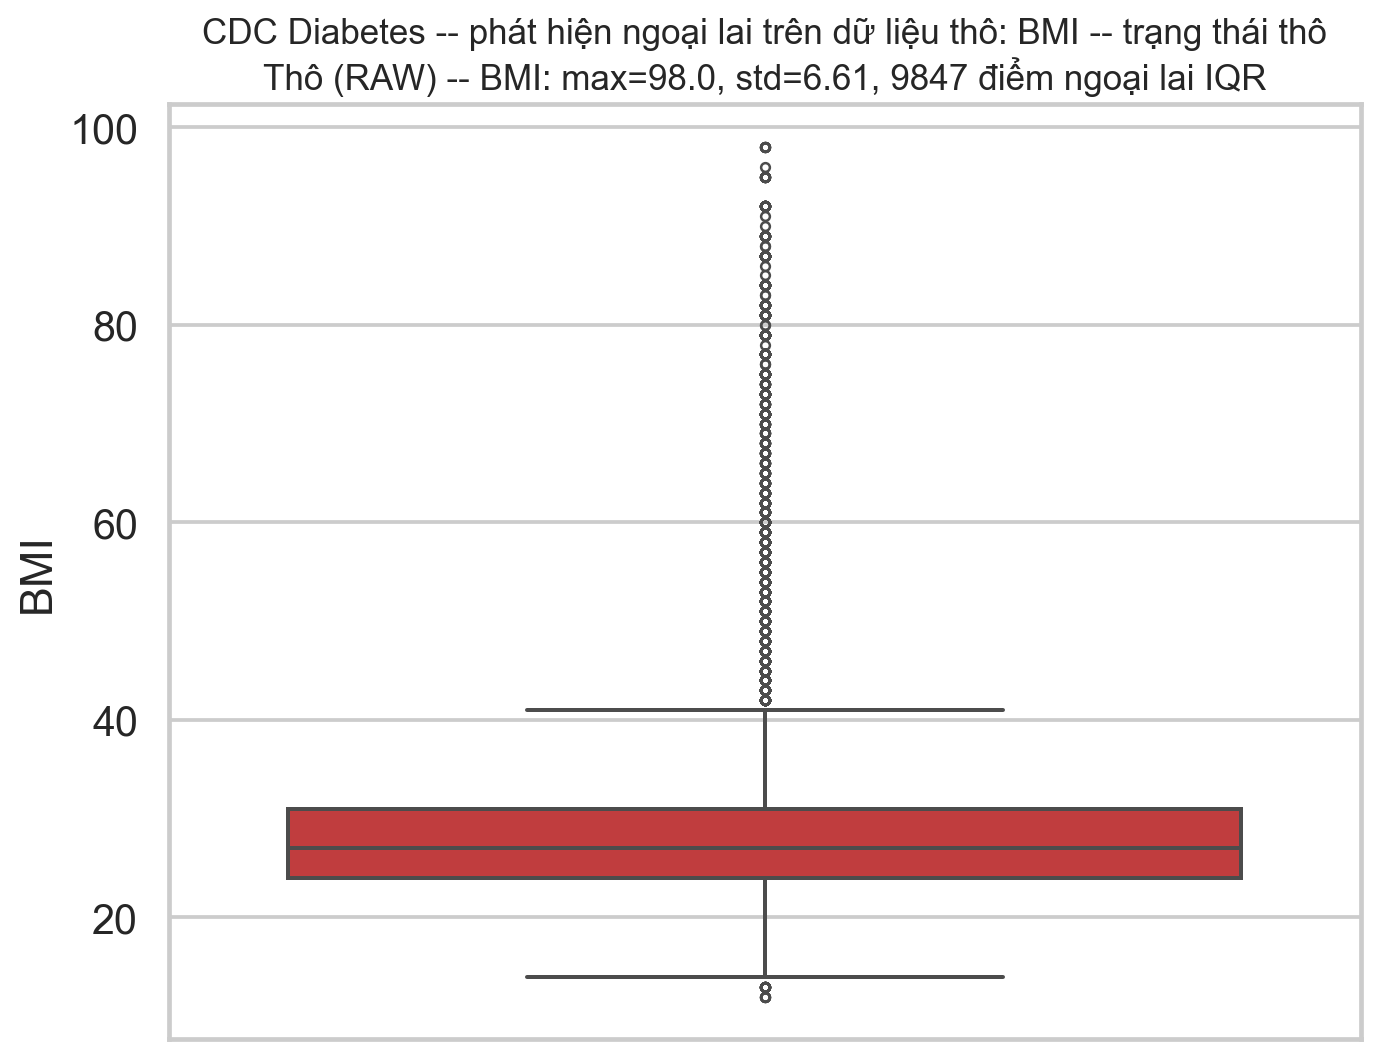
\includegraphics[width=0.72\textwidth]{images/ch3/cdc_diabetes_BMI_boxplot_raw.png}
\captionsetup{justification=raggedright,singlelinecheck=false}
\caption[Boxplot \texttt{BMI} thô CDC Diabetes]{Boxplot \texttt{BMI} CDC Diabetes ở \textbf{trạng thái thô}: hàng nghìn điểm ngoại lai ở đuôi phải tới BMI=98 (ngưỡng trên hộp $\approx 41.5$).\\
\footnotesize Python source: \texttt{scripts/generate\_raw\_vs\_cleaned\_boxplots.py}.}
\label{fig:ch4_cdc_raw_boxplot}
\end{figure}

\textit{Phát hiện ngoại lai trên dữ liệu thô (boxplot).} Dưới boxplot trạng thái thô (Hình~\ref{fig:ch4_cdc_raw_boxplot}), vấn đề chính là \emph{ngoại lai}: \texttt{BMI} có giá trị \textbf{tới 98} (béo phì bệnh lý cực đoan, so với $Q3+1.5IQR \approx 41.5$) -- hàng nghìn bệnh nhân nằm ngoài râu trên hộp ở đuôi phải; \texttt{MentHlth} và \texttt{PhysHlth} (số ngày sức khỏe tâm thần/thể chất kém trong 30 ngày) \textbf{chận 30 ngày}, gấp nhiều lần median=0, tạo các điểm rời rạc kéo dài từ giữa hộp đến giá trị cực đại; \texttt{Age} và \texttt{GenHlth} (ordinal) không có ngoại lai vì các giá trị đã nằm trong miền hợp lệ.

\textbf{Làm sạch dữ liệu.} Các bước làm sạch dữ liệu:

\begin{itemize}[leftmargin=*]
    \item \textbf{Phát hiện ngoại lai:} đã thực hiện ở trên qua boxplot -- chỉ ba biến \texttt{BMI}, \texttt{MentHlth}, \texttt{PhysHlth} có ngoại lai cực trị.
    \item \textbf{Xử lý ngoại lai:} \emph{clipping theo IQR} trên ba biến \texttt{BMI}, \texttt{MentHlth}, \texttt{PhysHlth} (ví dụ \texttt{BMI}=98 $\to$ 41.5, \texttt{MentHlth}/\texttt{PhysHlth} max 30 $\to$ 5.0/7.5).
    \item \textbf{Biến ordinal/nhị phân:} \texttt{Age}, \texttt{GenHlth} giữ nguyên mã lớp vì không có ngoại lai trong miền hợp lệ.
    \item \textbf{Điền khuyết:} \emph{không cần} -- dữ liệu thô không có ô NaN.
\end{itemize}

\begin{figure}[H]
\centering
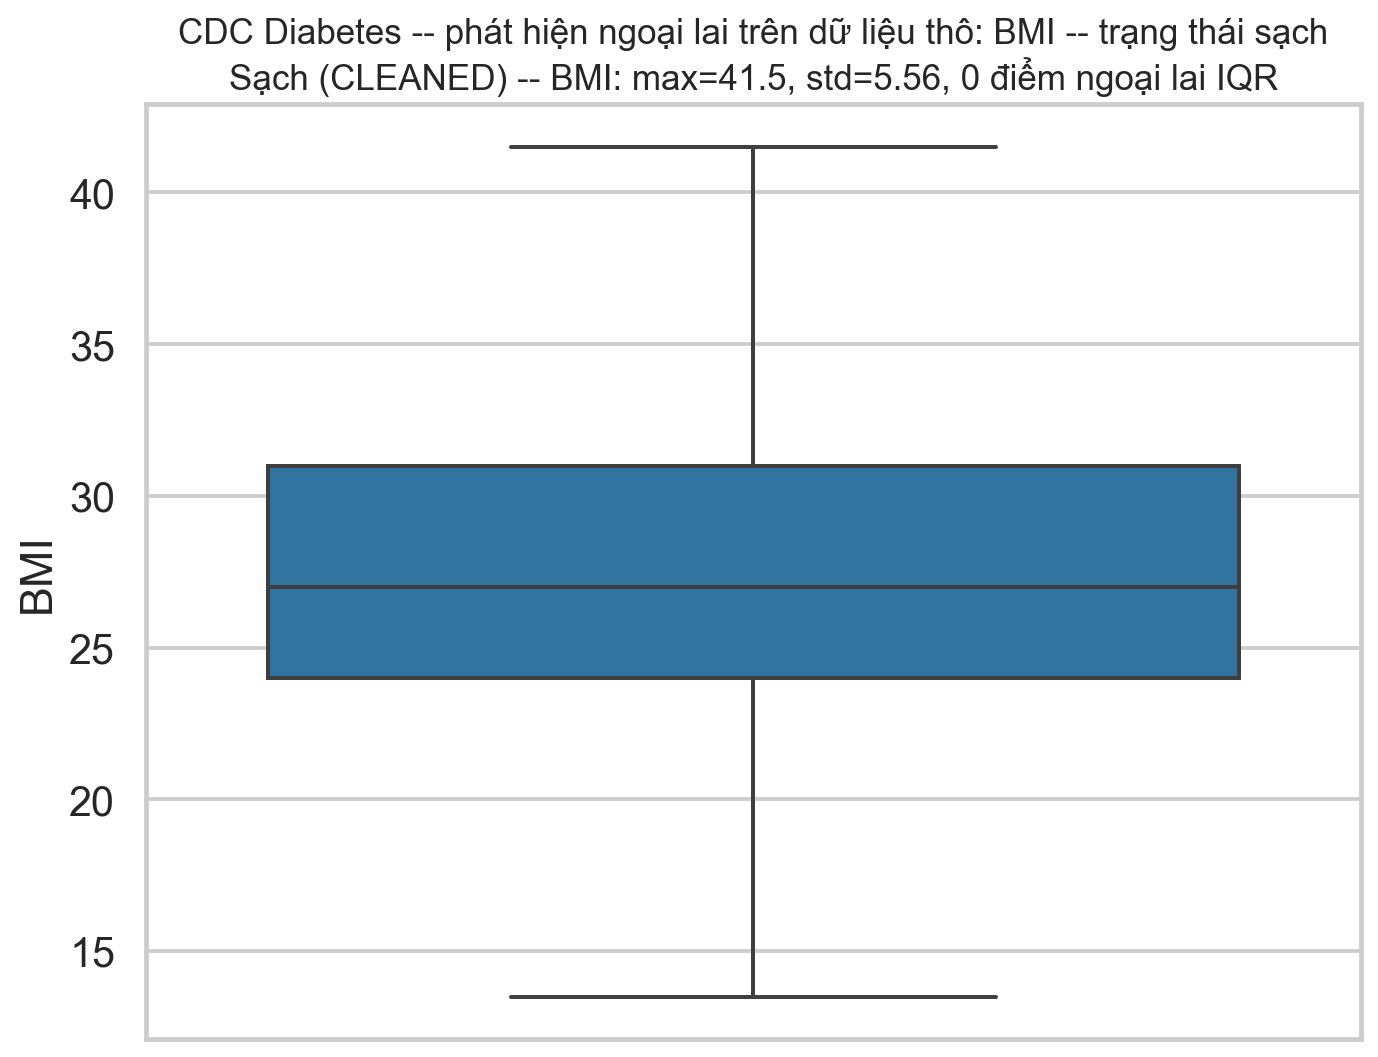
\includegraphics[width=0.72\textwidth]{images/ch3/cdc_diabetes_BMI_boxplot_cleaned.png}
\captionsetup{justification=raggedright,singlelinecheck=false}
\caption[Boxplot \texttt{BMI} sạch CDC Diabetes]{Boxplot \texttt{BMI} CDC Diabetes ở \textbf{trạng thái sạch}: sau clipping IQR, các điểm ngoại lai đuôi phải được nén về ngưỡng trên hộp, max giảm từ 98 xuống $\approx 41.5$.\\
\footnotesize Python source: \texttt{scripts/generate\_raw\_vs\_cleaned\_boxplots.py}.}
\label{fig:ch4_cdc_cleaned_boxplot}
\end{figure}

\textbf{Bước 1. Phân loại biến.}

\begin{table}[H]
\centering
\caption{Bước 1 -- Phân loại biến tiêu biểu trong CDC Diabetes}
\label{tab:ch4_cdc_variable_types}
\small
\begin{tabularx}{\textwidth}{p{0.18\textwidth}p{0.27\textwidth}p{0.25\textwidth}Y}
\toprule
Biến & Bản chất & Thống kê dùng & Biểu đồ phù hợp \\
\midrule
\texttt{BMI} & Quantitative Continuous & Mean, median, IQR, dữ liệu bất thường & Histogram, boxplot \\
\texttt{Age} & Quantitative Discrete/ordinal & Tần suất, median, IQR & Bar chart, scatter \\
\texttt{GenHlth} & Ordinal & Mode, median, IQR & Bar chart, histogram rời rạc \\
\texttt{MentHlth} & Quantitative Discrete & Mean, median, CV & Histogram, boxplot \\
\texttt{PhysHlth} & Quantitative Discrete & Mean, median, CV & Histogram, boxplot \\
\texttt{HighBP} & Qualitative binary & Tần suất, tỷ lệ, mode & Bar chart theo target \\
\bottomrule
\end{tabularx}
\end{table}

Năm biến định lượng/thứ bậc được chọn gồm \texttt{BMI}, \texttt{GenHlth}, \texttt{MentHlth}, \texttt{PhysHlth}, \texttt{Age}; các biến nhị phân \texttt{HighBP}, \texttt{HighChol}, \texttt{PhysActivity}, \texttt{Smoker} được dùng để đọc cấu trúc tần suất và quan hệ với \texttt{Diabetes\_binary}.

\textbf{Bước 2. Bảng tần suất và thống kê mô tả.}

\begin{table}[H]
\centering
\caption[Thống kê mô tả các biến tiêu biểu CDC Diabetes]{Bước 2 -- Thống kê mô tả các biến Quantitative tiêu biểu CDC Diabetes: xu hướng trung tâm và độ phân tán. Source: \texttt{outputs/tables/cdc\_diabetes\_summary.csv}.}
\label{tab:ch4_cdc_stats}
\scriptsize
\setlength{\tabcolsep}{3pt}
\begin{tabular}{lrrrrrrrrrr}
\toprule
Biến & Mean & Med & Mode & P25 & P75 & Range & Var & Std & CV & IQR \\
\midrule
\texttt{BMI} & 28.38 & 27.00 & 27.00 & 24.00 & 31.00 & 86.00 & 43.67 & 6.61 & 0.233 & 7.00 \\
\texttt{GenHlth} & 2.51 & 2.00 & 2.00 & 2.00 & 3.00 & 4.00 & 1.14 & 1.07 & 0.425 & 1.00 \\
\texttt{MentHlth} & 3.18 & 0.00 & 0.00 & 0.00 & 2.00 & 30.00 & 54.95 & 7.41 & 2.328 & 2.00 \\
\texttt{PhysHlth} & 4.24 & 0.00 & 0.00 & 0.00 & 3.00 & 30.00 & 76.00 & 8.72 & 2.055 & 3.00 \\
\texttt{Age} & 8.03 & 8.00 & 9.00 & 6.00 & 10.00 & 12.00 & 9.33 & 3.05 & 0.380 & 4.00 \\
\bottomrule
\end{tabular}
\end{table}

\begin{table}[H]
\centering
\caption[Thống kê thô/sạch CDC Diabetes]{So sánh thống kê mô tả CDC Diabetes ở hai trạng thái: \textbf{thô} và \textbf{sạch} (clipping IQR trên \texttt{BMI}, \texttt{MentHlth}, \texttt{PhysHlth}). Các cột in đậm thay đổi nhiều nhất. Source: \texttt{outputs/tables/cdc\_diabetes\_summary.csv}.}
\label{tab:ch4_cdc_stats_raw_clean}
\footnotesize
\setlength{\tabcolsep}{4pt}
\begin{tabular}{lcrrrrrr}
\toprule
Biến & Trạng thái & Mean & Median & \textbf{Std} & \textbf{Max} & \textbf{Range} & IQR \\
\midrule
\texttt{BMI} & thô & 28.38 & 27.00 & \textbf{6.61} & \textbf{98.00} & \textbf{86.00} & 7.00 \\
 & sạch & 28.11 & 27.00 & \textbf{5.56} & \textbf{41.50} & \textbf{28.00} & 7.00 \\
\midrule
\texttt{GenHlth} & thô & 2.51 & 2.00 & 1.07 & 5.00 & 4.00 & 1.00 \\
 & sạch & 2.51 & 2.00 & 1.07 & 5.00 & 4.00 & 1.00 \\
\midrule
\texttt{MentHlth} & thô & 3.18 & 0.00 & \textbf{7.41} & \textbf{30.00} & \textbf{30.00} & 2.00 \\
 & sạch & 1.18 & 0.00 & \textbf{1.95} & \textbf{5.00} & \textbf{5.00} & 2.00 \\
\midrule
\texttt{PhysHlth} & thô & 4.24 & 0.00 & \textbf{8.72} & \textbf{30.00} & \textbf{30.00} & 3.00 \\
 & sạch & 1.85 & 0.00 & \textbf{2.89} & \textbf{7.50} & \textbf{7.50} & 3.00 \\
\midrule
\texttt{Age} & thô & 8.03 & 8.00 & 3.05 & 13.00 & 12.00 & 4.00 \\
 & sạch & 8.03 & 8.00 & 3.05 & 13.00 & 12.00 & 4.00 \\
\bottomrule
\end{tabular}
\end{table}

\textit{Nhận xét thô/sạch.} CDC Diabetes thể hiện rõ nguyên tắc ``clipping chọn lọc'': \texttt{BMI} giảm std 15.9\% và max 57.7\% (98$\to$41.5); \texttt{MentHlth} và \texttt{PhysHlth} -- hai biến đếm có đuôi dài -- giảm std rất mạnh (73.7\% và 66.9\%) vì phần lớn giá trị cao (gần 30 ngày) bị nén về ngưỡng trên hộp. Trong khi đó \texttt{GenHlth} và \texttt{Age} (ordinal) giữ nguyên mọi chỉ số, do không có ngoại lai trong miền hợp lệ.

\begin{table}[H]
\centering
\caption[Bảng tần suất biến \texttt{HighBP} trong CDC Diabetes]{Bảng tần suất biến \texttt{HighBP} trong CDC Diabetes. Source: \texttt{outputs/tables/cdc\_diabetes\_frequency\_HighBP.csv}.}
\label{tab:ch4_cdc_frequency}
\small
\begin{tabular}{lrr}
\toprule
\texttt{HighBP} & Tần suất tuyệt đối & Tần suất tương đối \\
\midrule
0 (không huyết áp cao) & 144\,851 & 57.10\% \\
1 (có huyết áp cao) & 108\,829 & 42.90\% \\
\bottomrule
\end{tabular}
\end{table}

\textbf{Bước 3. Trực quan hóa dữ liệu.} Tương tự Heart Disease, hệ thống biểu đồ của CDC Diabetes được chọn theo bản chất biến: bar chart cho biến nhị phân \texttt{HighBP}, histogram và boxplot cho \texttt{BMI}, scatter plot cho quan hệ \texttt{Age}--\texttt{BMI}, biểu đồ phân bố target để kiểm tra mất cân bằng lớp và heatmap để khảo sát tương quan giữa các yếu tố nguy cơ chuyển hóa.

\begin{figure}[H]
\centering
\begin{subfigure}{0.90\textwidth}
 \centering
 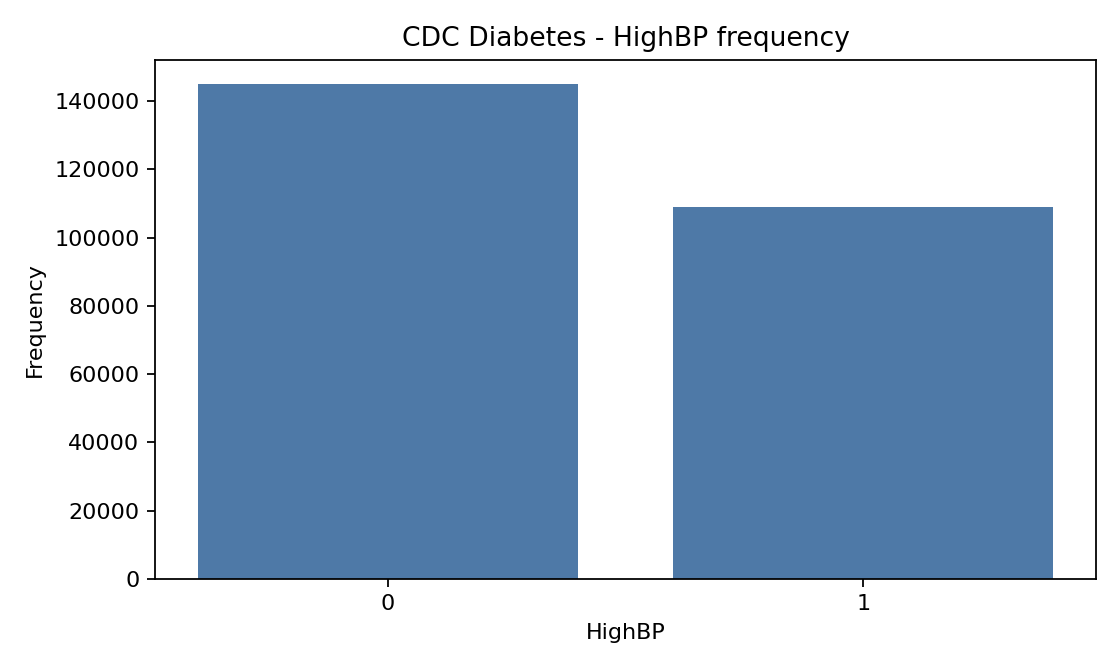
\includegraphics[width=\textwidth]{images/ch3/cdc_diabetes_highbp_bar.png}
 \caption{Python -- Bar chart \texttt{HighBP}}
\end{subfigure}
\par\medskip
\begin{subfigure}{0.90\textwidth}
 \centering
 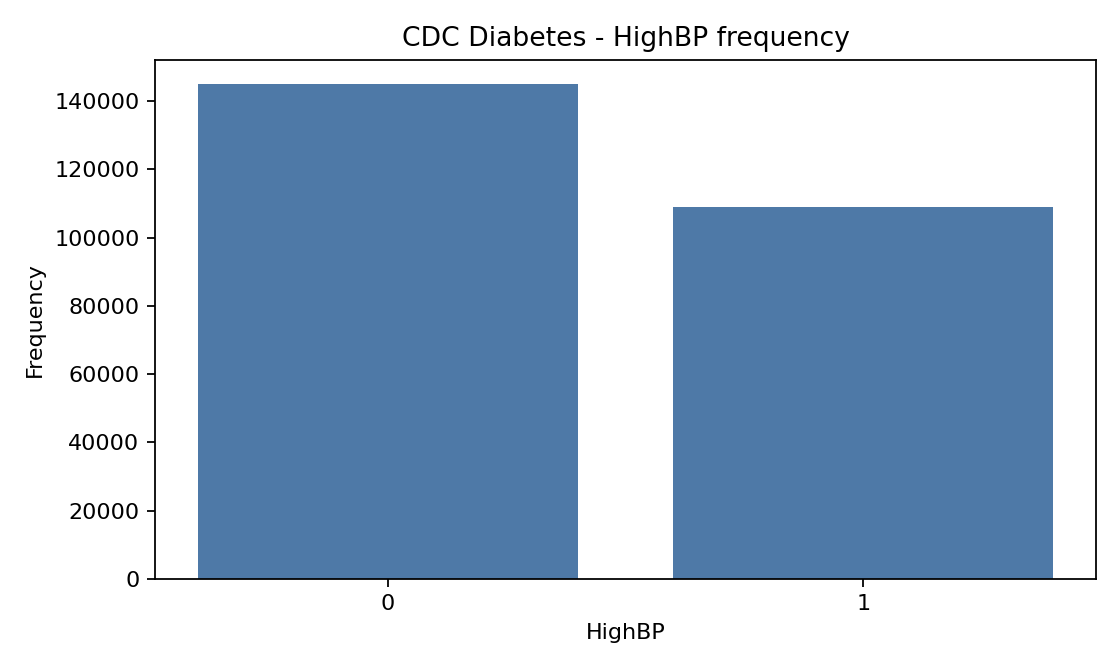
\includegraphics[width=\textwidth]{images/ch3/excel_cdc_highbp_bar_preview.png}
 \caption{Excel -- Column chart \texttt{HighBP}}
\end{subfigure}
\captionsetup{justification=raggedright,singlelinecheck=false}
\caption[Bar chart \texttt{HighBP} CDC Diabetes: Python và Excel]{Tần suất huyết áp cao trong CDC Diabetes, đối chiếu giữa Python và Excel.\\
\footnotesize Python source: \texttt{src/analyze\_cdc\_diabetes.py}.\\
Excel source/workbook: \texttt{src/create\_excel\_visualizations.py}, \texttt{excel/excel\_visualization\_comparison\_native.xlsx}, sheet \texttt{CDC HighBP}.}
\label{fig:ch4_cdc_highbp_bar}
\end{figure}

\textbf{Nhận xét Hình \ref{fig:ch4_cdc_highbp_bar}.} Biến \texttt{HighBP} có tỷ lệ có huyết áp cao 42.90\%, đủ lớn để trở thành tín hiệu nguy cơ quan trọng. Vì đây là biến nhị phân định tính, tần suất tuyệt đối, tần suất tương đối và mode phù hợp hơn mean/median.

\begin{figure}[H]
\centering
\begin{subfigure}{0.90\textwidth}
 \centering
 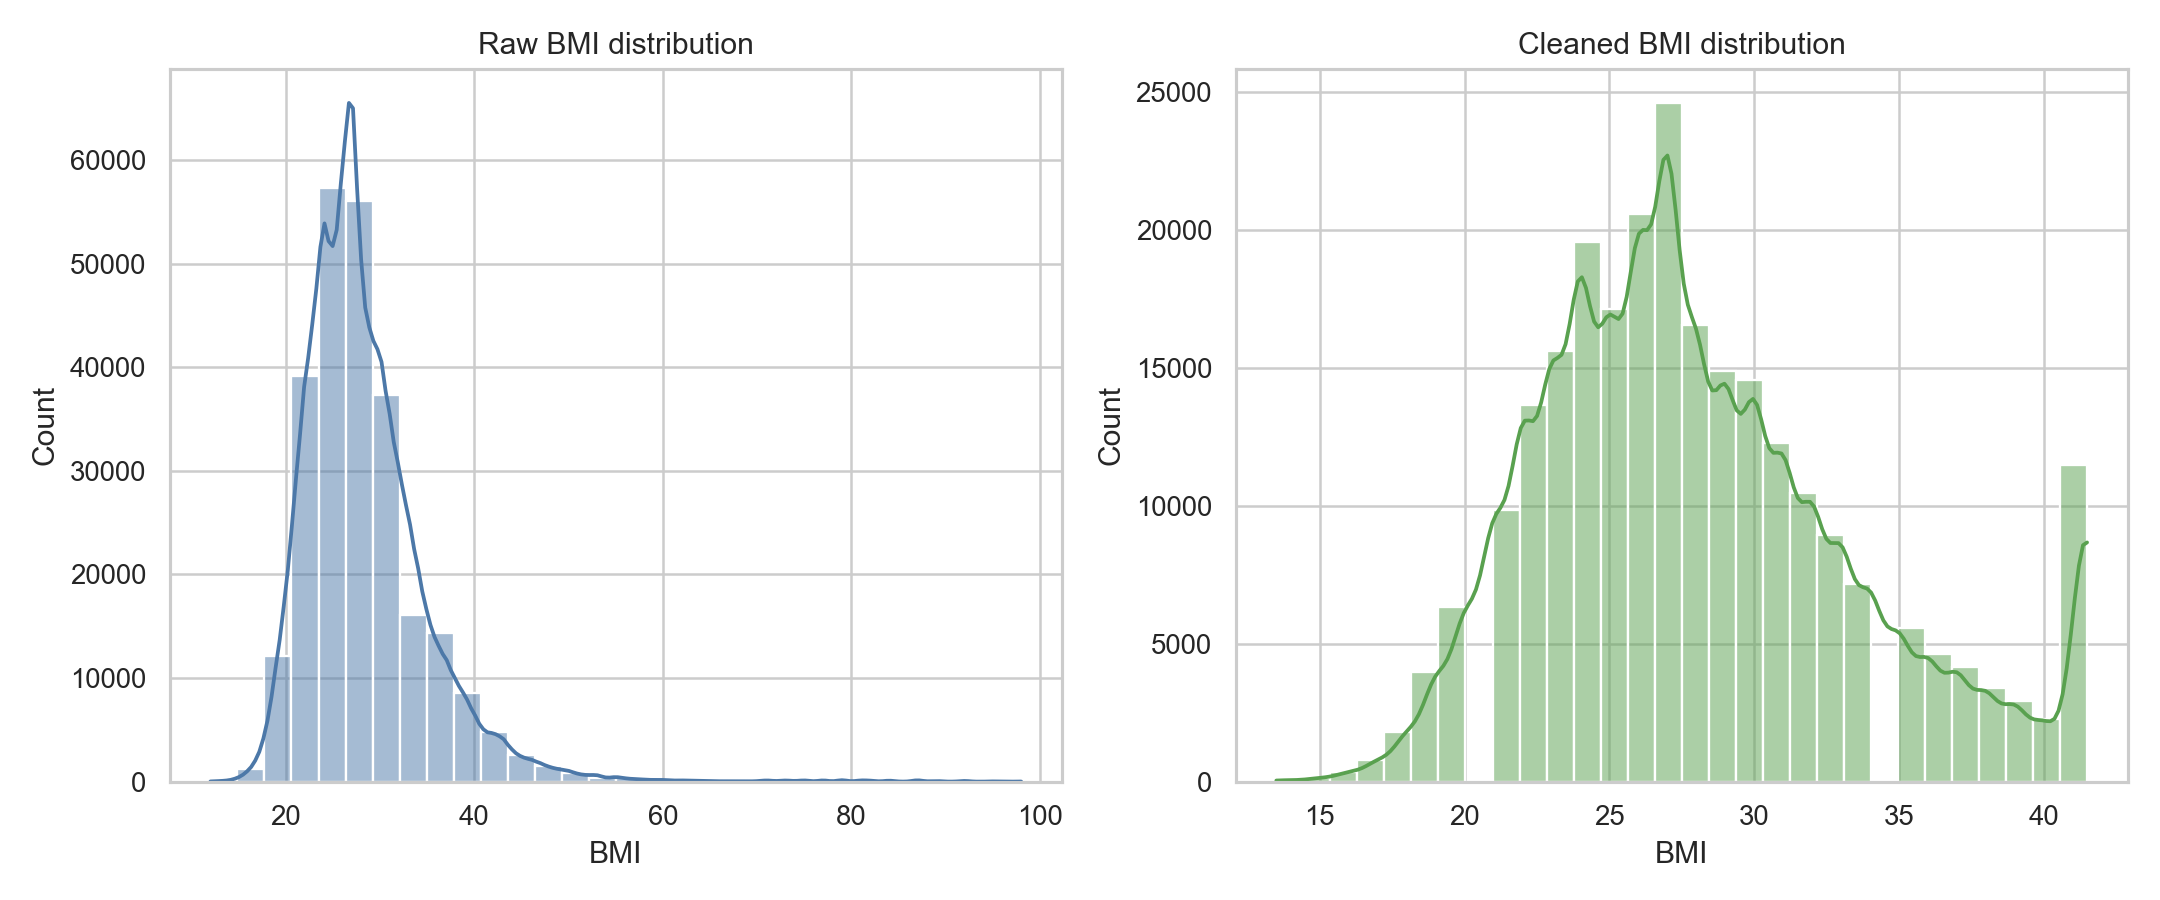
\includegraphics[width=\textwidth]{images/ch3/cdc_diabetes_bmi_raw_vs_cleaned.png}
 \caption{Python -- Histogram \texttt{BMI} thô/sạch}
\end{subfigure}
\par\medskip
\begin{subfigure}{0.90\textwidth}
 \centering
 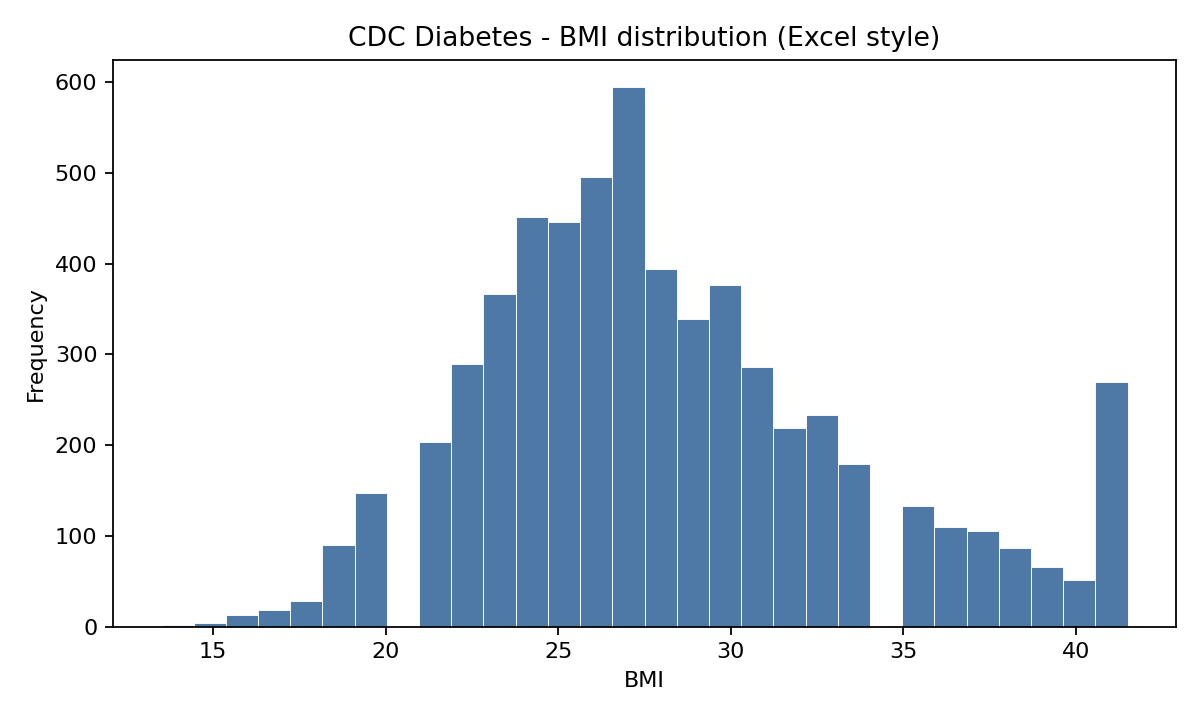
\includegraphics[width=\textwidth]{images/ch3/excel_cdc_bmi_raw_vs_cleaned_preview.png}
 \caption{Excel -- Histogram \texttt{BMI}}
\end{subfigure}
\captionsetup{justification=raggedright,singlelinecheck=false}
\caption[Histogram \texttt{BMI} CDC Diabetes: Python và Excel]{Phân phối \texttt{BMI} sau tiền xử lý trong CDC Diabetes, đối chiếu giữa Python và Excel.\\
\footnotesize Python source: \texttt{src/analyze\_cdc\_diabetes.py}.\\
Excel source/workbook: \texttt{src/create\_excel\_visualizations.py}, \texttt{excel/excel\_visualization\_comparison\_native.xlsx}, sheet \texttt{CDC BMI Hist}.}
\label{fig:ch4_cdc_bmi_hist}
\end{figure}

\textbf{Nhận xét Hình \ref{fig:ch4_cdc_bmi_hist}.} Histogram \texttt{BMI} cho thấy tiền xử lý làm đuôi phải ngắn hơn: max giảm từ 98 xuống 41.5 và độ lệch chuẩn giảm từ 6.61 xuống 5.56. Như vậy dữ liệu sau xử lý có phân phối mượt và ít bị chi phối bởi vài quan sát cực trị hơn dữ liệu thô.

\begin{figure}[H]
\centering
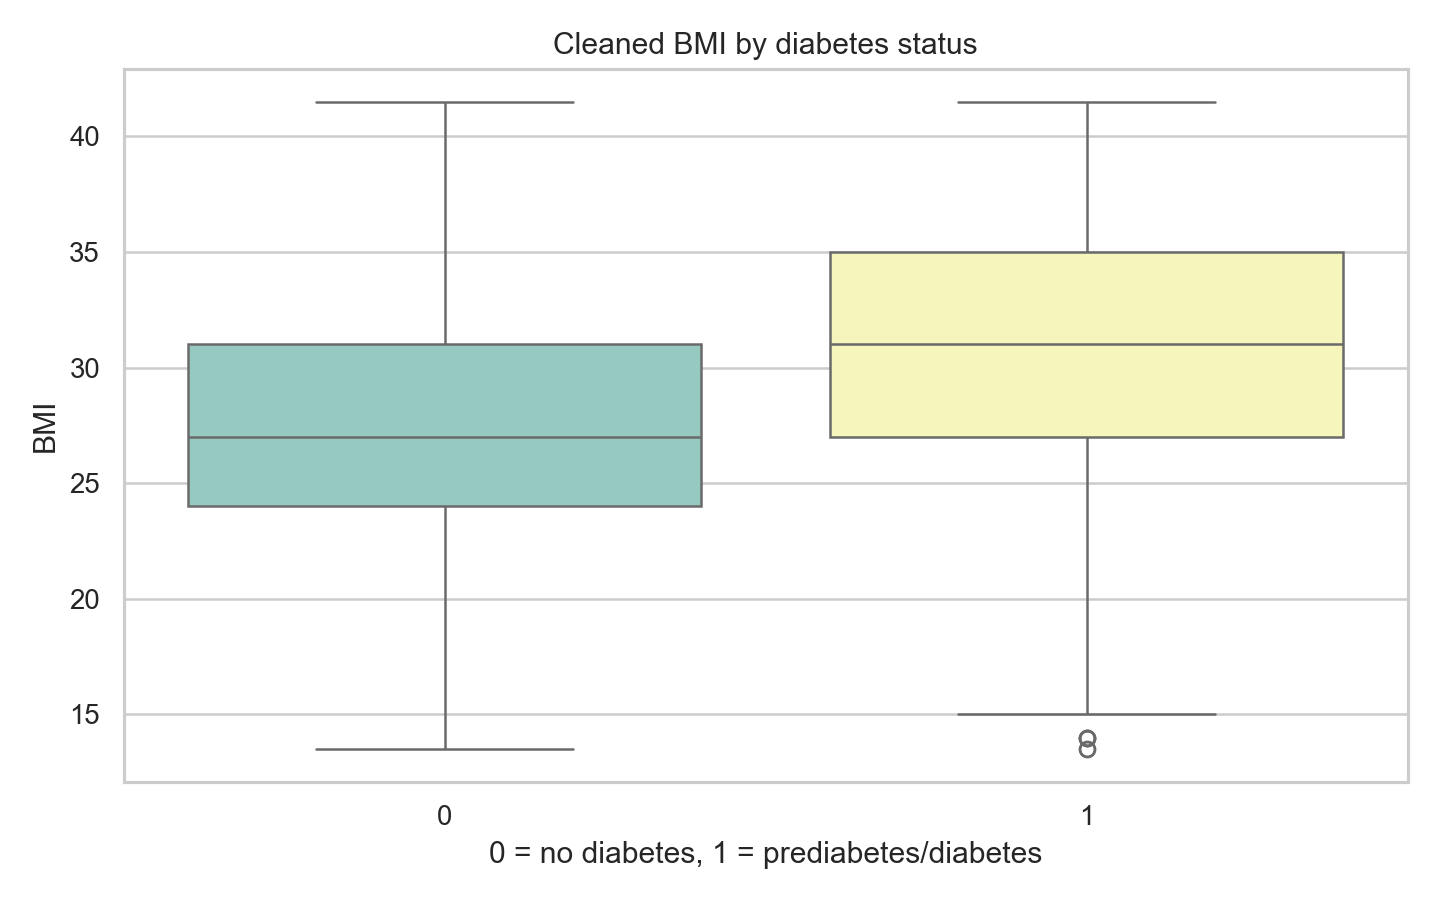
\includegraphics[width=0.90\textwidth]{images/ch3/cdc_diabetes_bmi_boxplot_by_target.png}
\captionsetup{justification=raggedright,singlelinecheck=false}
\caption[Boxplot \texttt{BMI} CDC Diabetes]{Boxplot \texttt{BMI} theo \texttt{Diabetes\_binary}.\\
\footnotesize Python source: \texttt{src/analyze\_cdc\_diabetes.py}.}
\label{fig:ch4_cdc_bmi_boxplot}
\end{figure}

\textbf{Nhận xét Hình \ref{fig:ch4_cdc_bmi_boxplot}.} Nhóm có tiểu đường có trung vị \texttt{BMI} cao hơn, dù hai hộp vẫn chồng lấn nhiều. Điều này cho thấy \texttt{BMI} có tín hiệu nhưng không đủ để phân loại đơn biến.

\textit{Đối chiếu thô/sạch.} Hai biểu đồ tiếp theo đặt dữ liệu thô (đỏ) cạnh dữ liệu sạch (xanh), qua đó thể hiện trực quan tác động của clipping IQR trên \texttt{BMI}.

\begin{figure}[H]
\centering
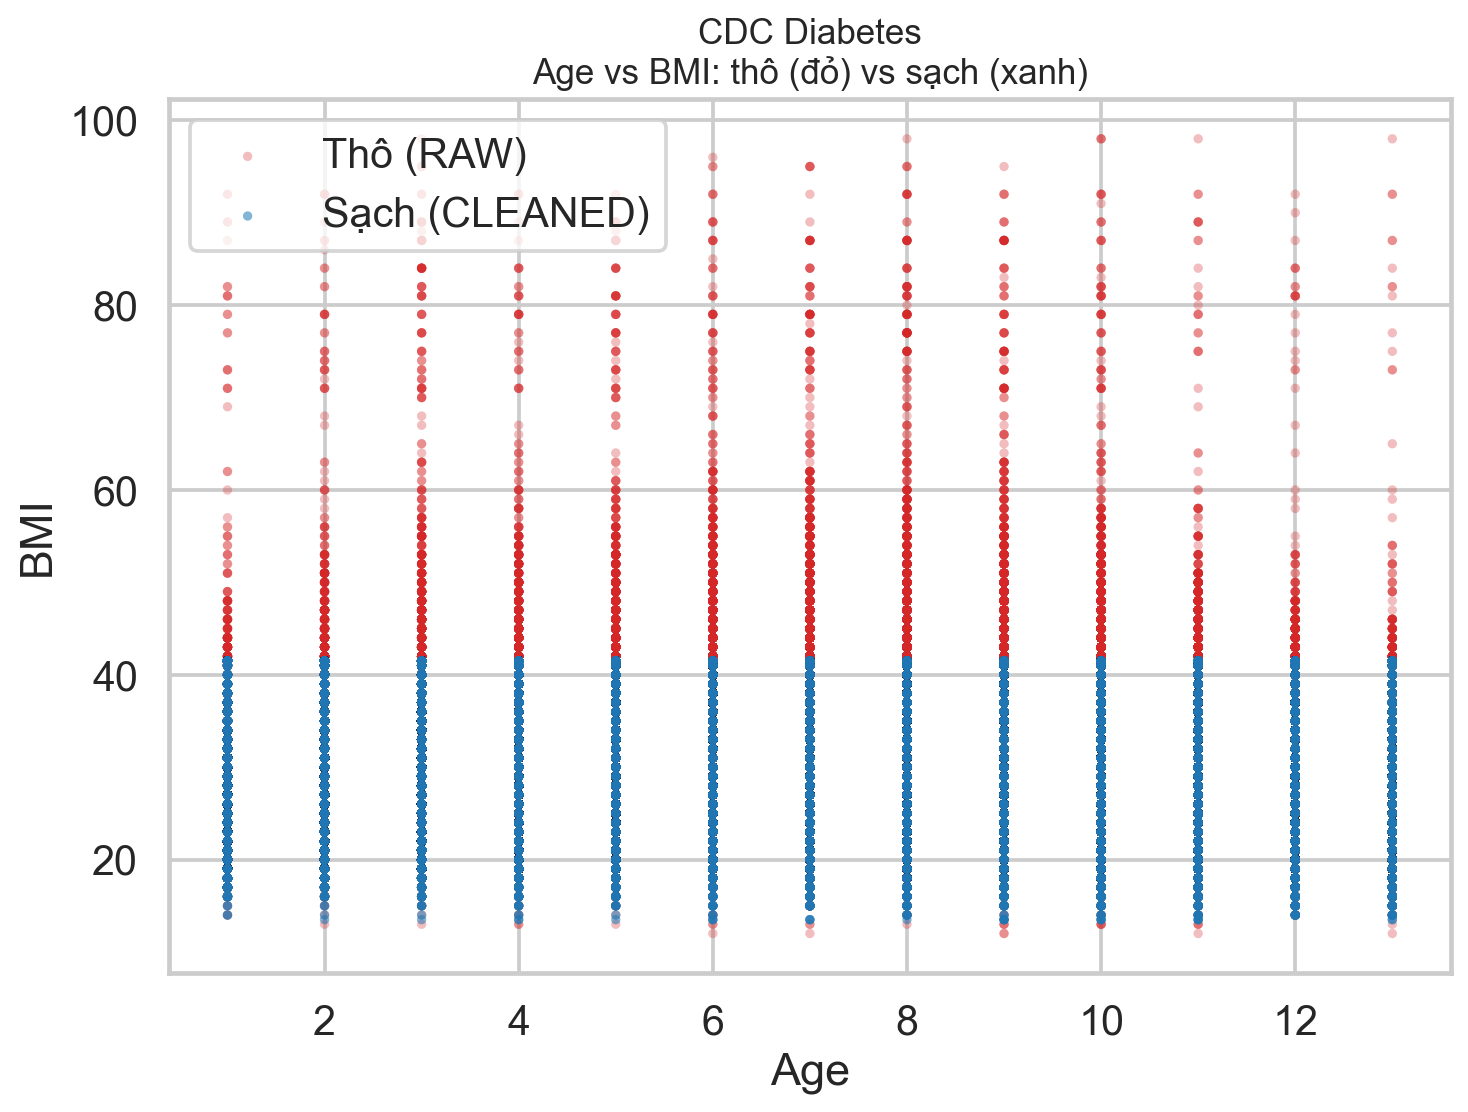
\includegraphics[width=0.82\textwidth]{images/ch3/cdc_diabetes_age_bmi_scatter_raw_vs_cleaned.png}
\captionsetup{justification=raggedright,singlelinecheck=false}
\caption[Scatter \texttt{Age}--\texttt{BMI} thô/sạch CDC Diabetes]{Scatter \texttt{Age}--\texttt{BMI} CDC Diabetes: dữ liệu thô (đỏ, mờ) phủ rộng tới BMI=98; dữ liệu sạch (xanh) bị nén về $\approx$41.5 -- vùng trên bị cắt rõ.\\
\footnotesize Python source: \texttt{scripts/generate\_raw\_vs\_cleaned\_boxplots.py}.}
\label{fig:ch4_cdc_scatter_compare}
\end{figure}

\begin{figure}[H]
\centering
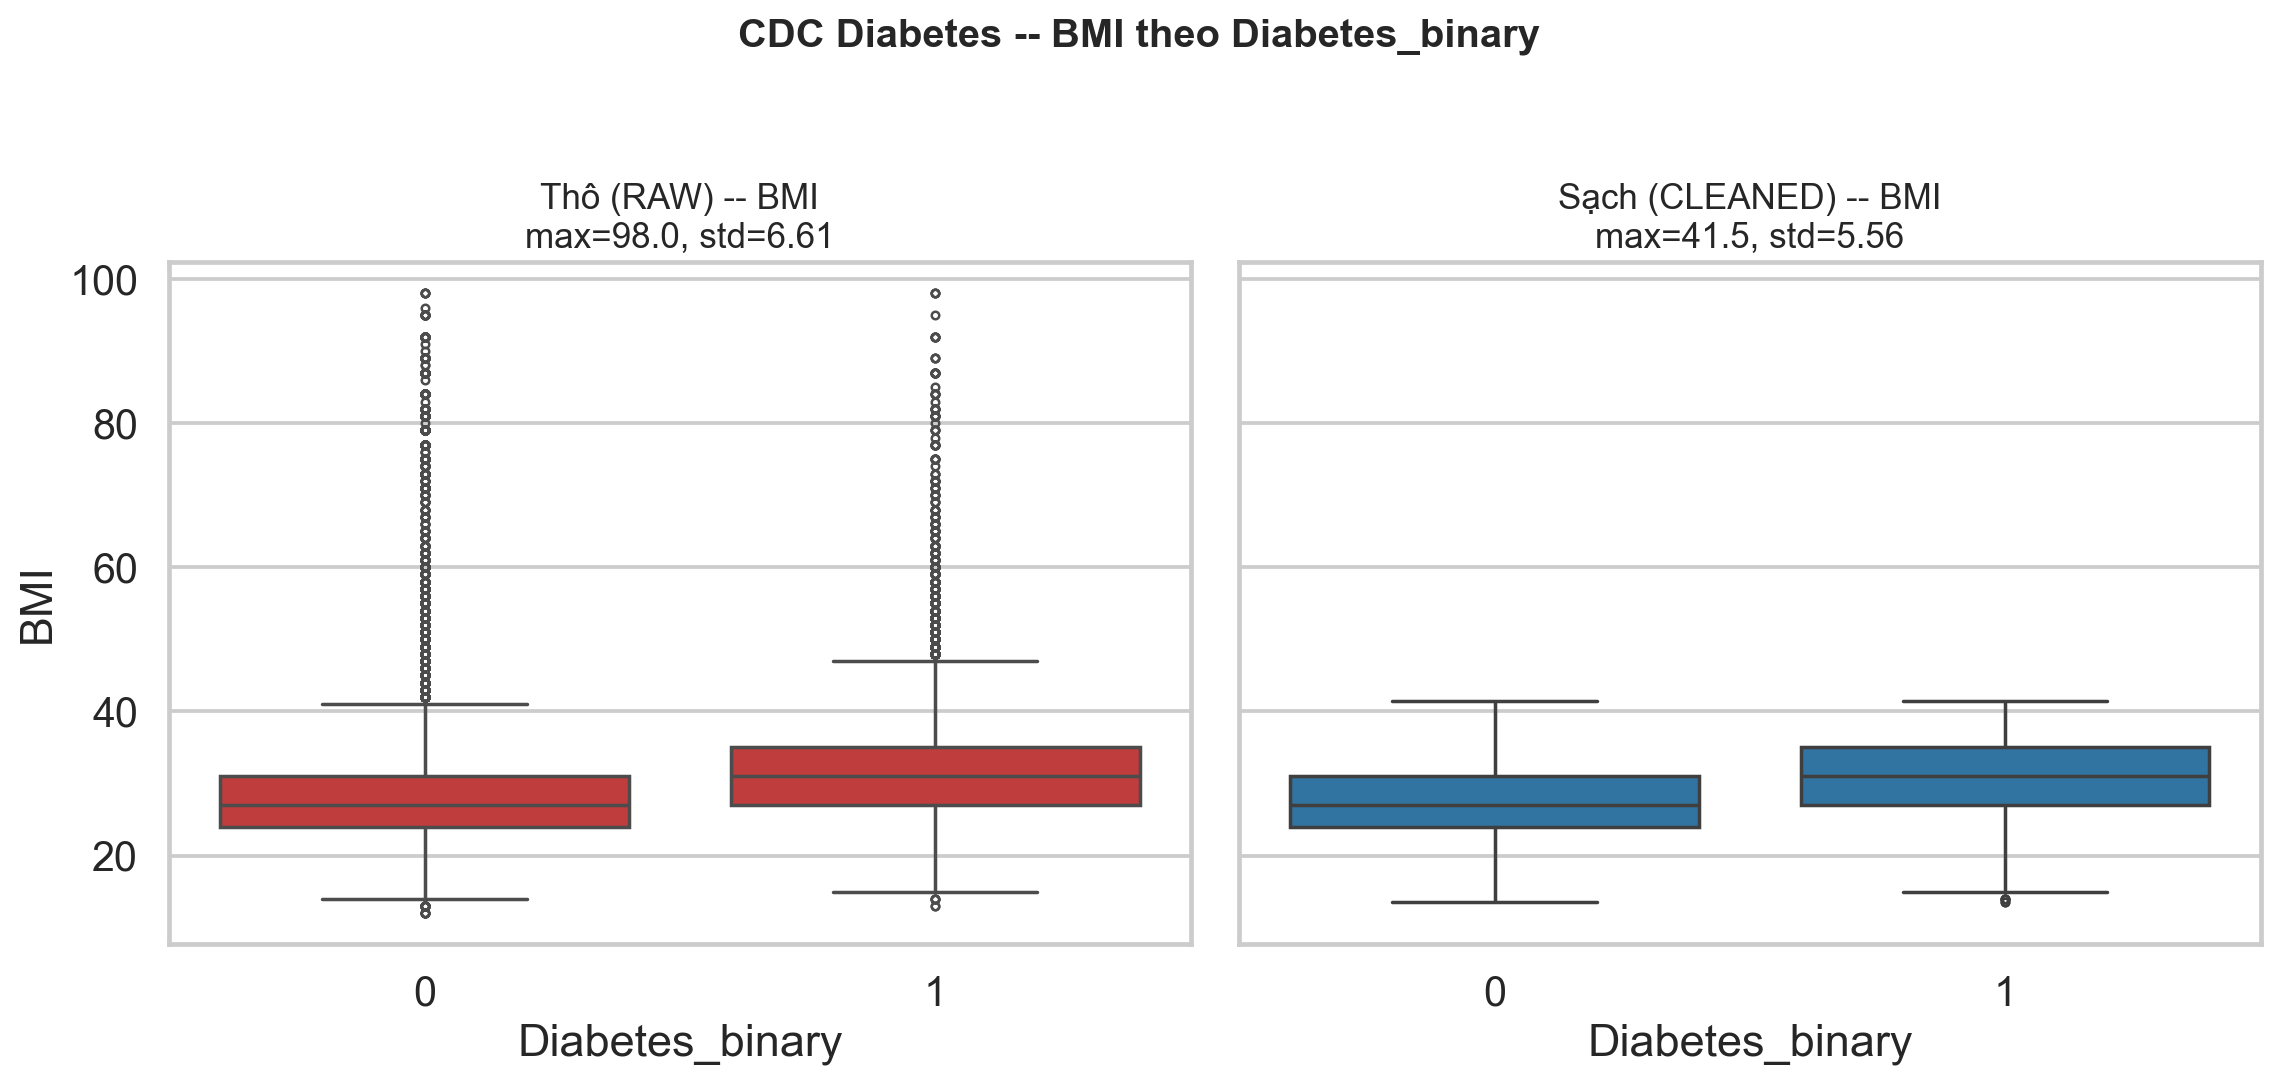
\includegraphics[width=0.95\textwidth]{images/ch3/cdc_diabetes_BMI_boxplot_by_target_raw_vs_cleaned.png}
\captionsetup{justification=raggedright,singlelinecheck=false}
\caption[Boxplot \texttt{BMI} theo target thô/sạch CDC Diabetes]{Boxplot \texttt{BMI} theo \texttt{Diabetes\_binary}: thô (trái) có hàng nghìn điểm ngoại lai tới 98; sạch (phải) sau clipping giảm ngoại lai nhưng trung vị nhóm tiểu đường vẫn cao hơn.\\
\footnotesize Python source: \texttt{scripts/generate\_raw\_vs\_cleaned\_boxplots.py}.}
\label{fig:ch4_cdc_boxplot_by_target_compare}
\end{figure}

\textbf{Nhận xét.} Scatter \texttt{Age}--\texttt{BMI} (Hình~\ref{fig:ch4_cdc_scatter_compare}) cho thấy vùng BMI$>$41.5 của dữ liệu thô (đỏ) biến mất ở dữ liệu sạch (xanh), nhưng phần lõi phân bố vẫn trùng nhau. Boxplot theo target (Hình~\ref{fig:ch4_cdc_boxplot_by_target_compare}) xác nhận sau clipping, hàng nghìn điểm ngoài râu bị nén, nhưng trung vị nhóm tiểu đường vẫn cao hơn nhóm không tiểu đường -- tín hiệu nguy cơ chuyển hóa được giữ nguyên.

\begin{figure}[H]
\centering
\begin{subfigure}{0.90\textwidth}
 \centering
 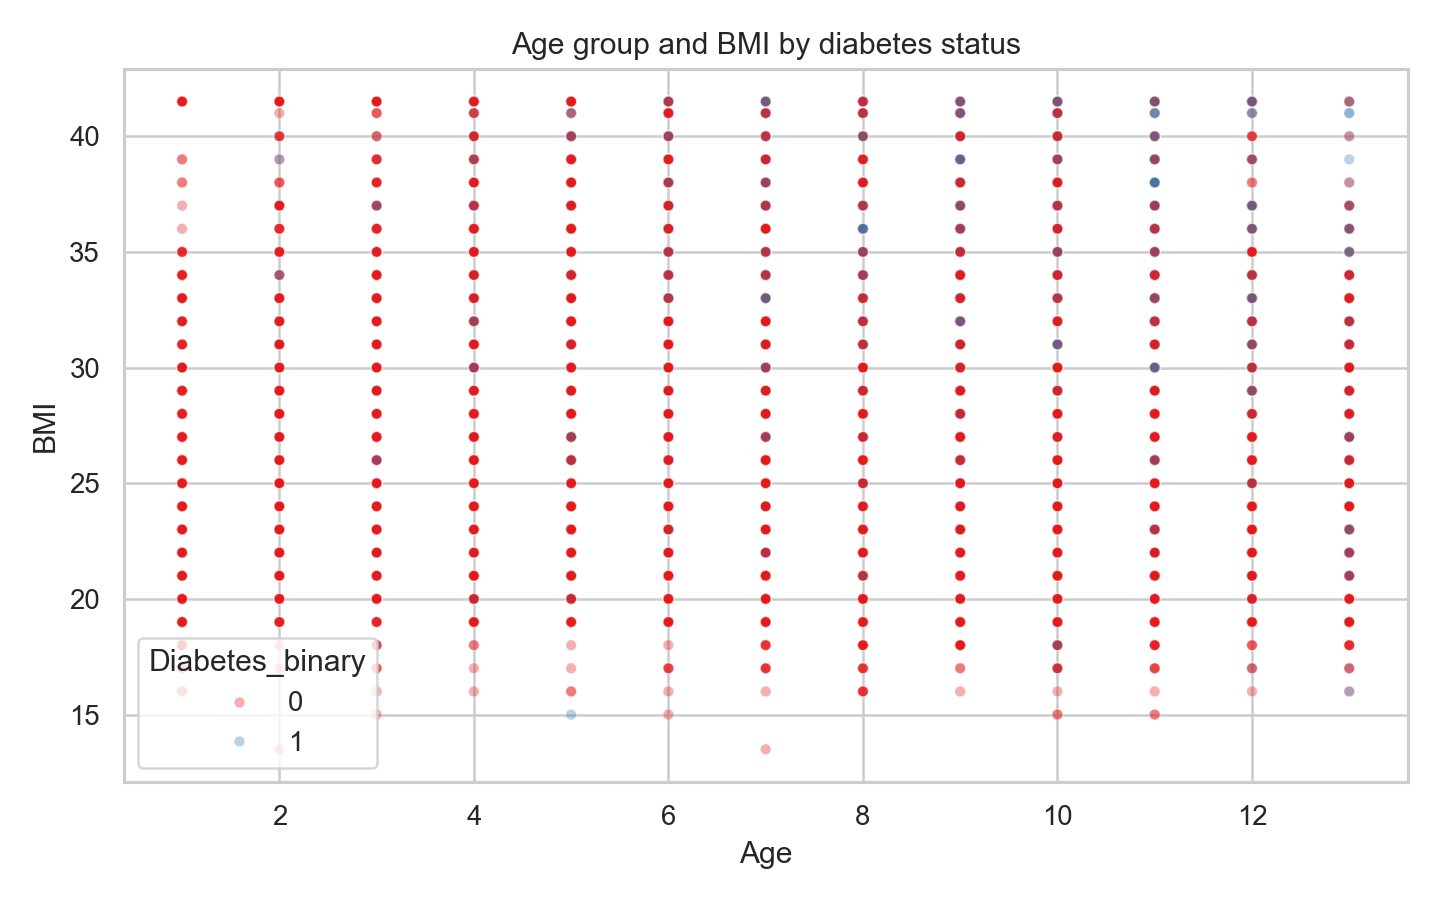
\includegraphics[width=\textwidth]{images/ch3/cdc_diabetes_age_bmi_scatter.png}
 \caption{Python -- Scatter \texttt{Age}--\texttt{BMI}}
\end{subfigure}
\par\medskip
\begin{subfigure}{0.90\textwidth}
 \centering
 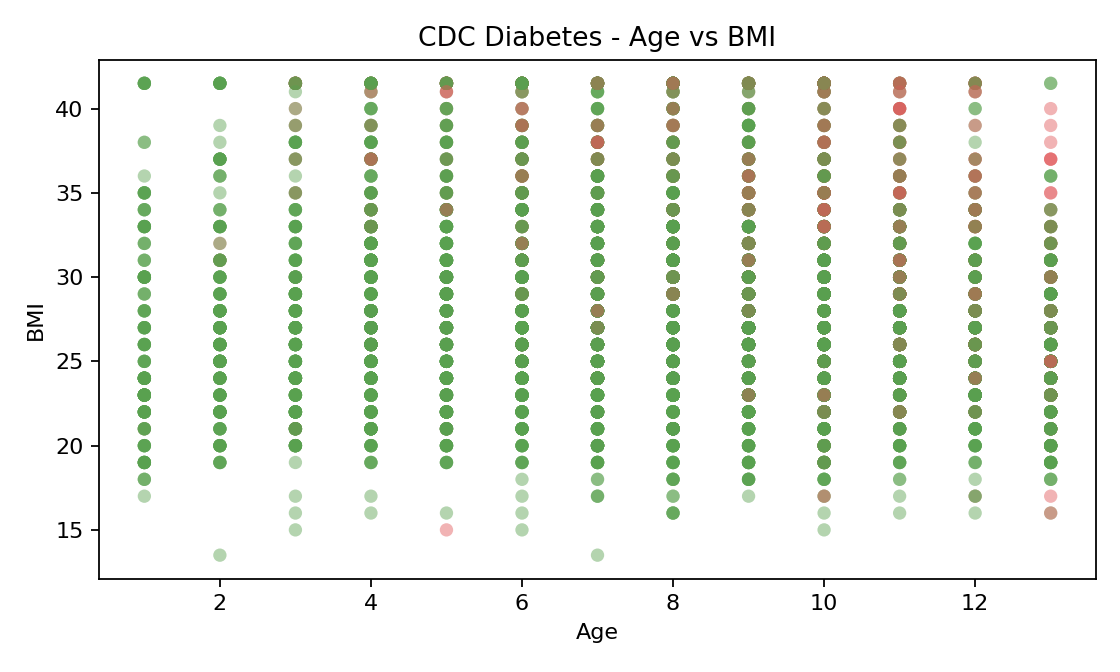
\includegraphics[width=\textwidth]{images/ch3/excel_cdc_age_bmi_scatter_preview.png}
 \caption{Excel -- Scatter \texttt{Age}--\texttt{BMI}}
\end{subfigure}
\captionsetup{justification=raggedright,singlelinecheck=false}
\caption[Scatter \texttt{Age}--\texttt{BMI} CDC Diabetes: Python và Excel]{Quan hệ giữa nhóm tuổi và BMI trong CDC Diabetes.\\
\footnotesize Python source: \texttt{src/analyze\_cdc\_diabetes.py}.\\
Excel source/workbook: \texttt{src/create\_excel\_visualizations.py}, \texttt{excel/excel\_visualization\_comparison\_native.xlsx}, sheet \texttt{CDC Age BMI}.}
\label{fig:ch4_cdc_age_bmi}
\end{figure}

\textbf{Nhận xét Hình \ref{fig:ch4_cdc_age_bmi}.} Scatter \texttt{Age}--\texttt{BMI} cho thấy dữ liệu phủ rộng ở nhiều nhóm tuổi; BMI cao xuất hiện ở nhiều mức tuổi thay vì chỉ tập trung ở một nhóm.

\begin{figure}[H]
\centering
\begin{subfigure}{0.90\textwidth}
 \centering
 \includegraphics[width=\textwidth]{images/ch3/cdc_diabetes_target_distribution.png}
 \caption{Python -- Phân bố \texttt{Diabetes\_binary}}
\end{subfigure}
\par\medskip
\begin{subfigure}{0.90\textwidth}
 \centering
 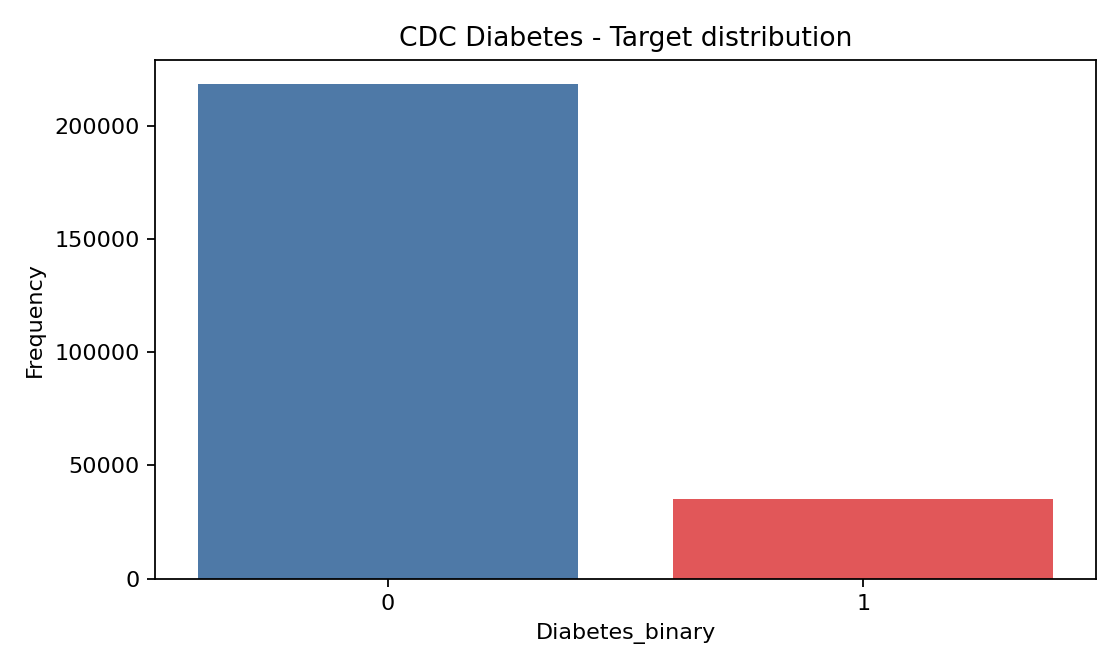
\includegraphics[width=\textwidth]{images/ch3/excel_cdc_target_distribution_preview.png}
 \caption{Excel -- Phân bố \texttt{Diabetes\_binary}}
\end{subfigure}
\captionsetup{justification=raggedright,singlelinecheck=false}
\caption[Phân bố target CDC Diabetes: Python và Excel]{Phân bố biến mục tiêu \texttt{Diabetes\_binary}, đối chiếu giữa Python và Excel.\\
\footnotesize Python source: \texttt{src/analyze\_cdc\_diabetes.py}.\\
Excel source/workbook: \texttt{src/create\_excel\_visualizations.py}, \texttt{excel/excel\_visualization\_comparison\_native.xlsx}, sheet \texttt{CDC Target}.}
\label{fig:ch4_cdc_target}
\end{figure}

\textbf{Nhận xét Hình \ref{fig:ch4_cdc_target}.} Phân bố target cho thấy lớp không tiểu đường chiếm ưu thế, dữ liệu mất cân bằng rõ rệt. Vì vậy, accuracy không đủ để đánh giá mô hình phân loại; cần đọc kèm precision, recall và F1, đặc biệt cho lớp tiểu đường.

\begin{figure}[H]
\centering
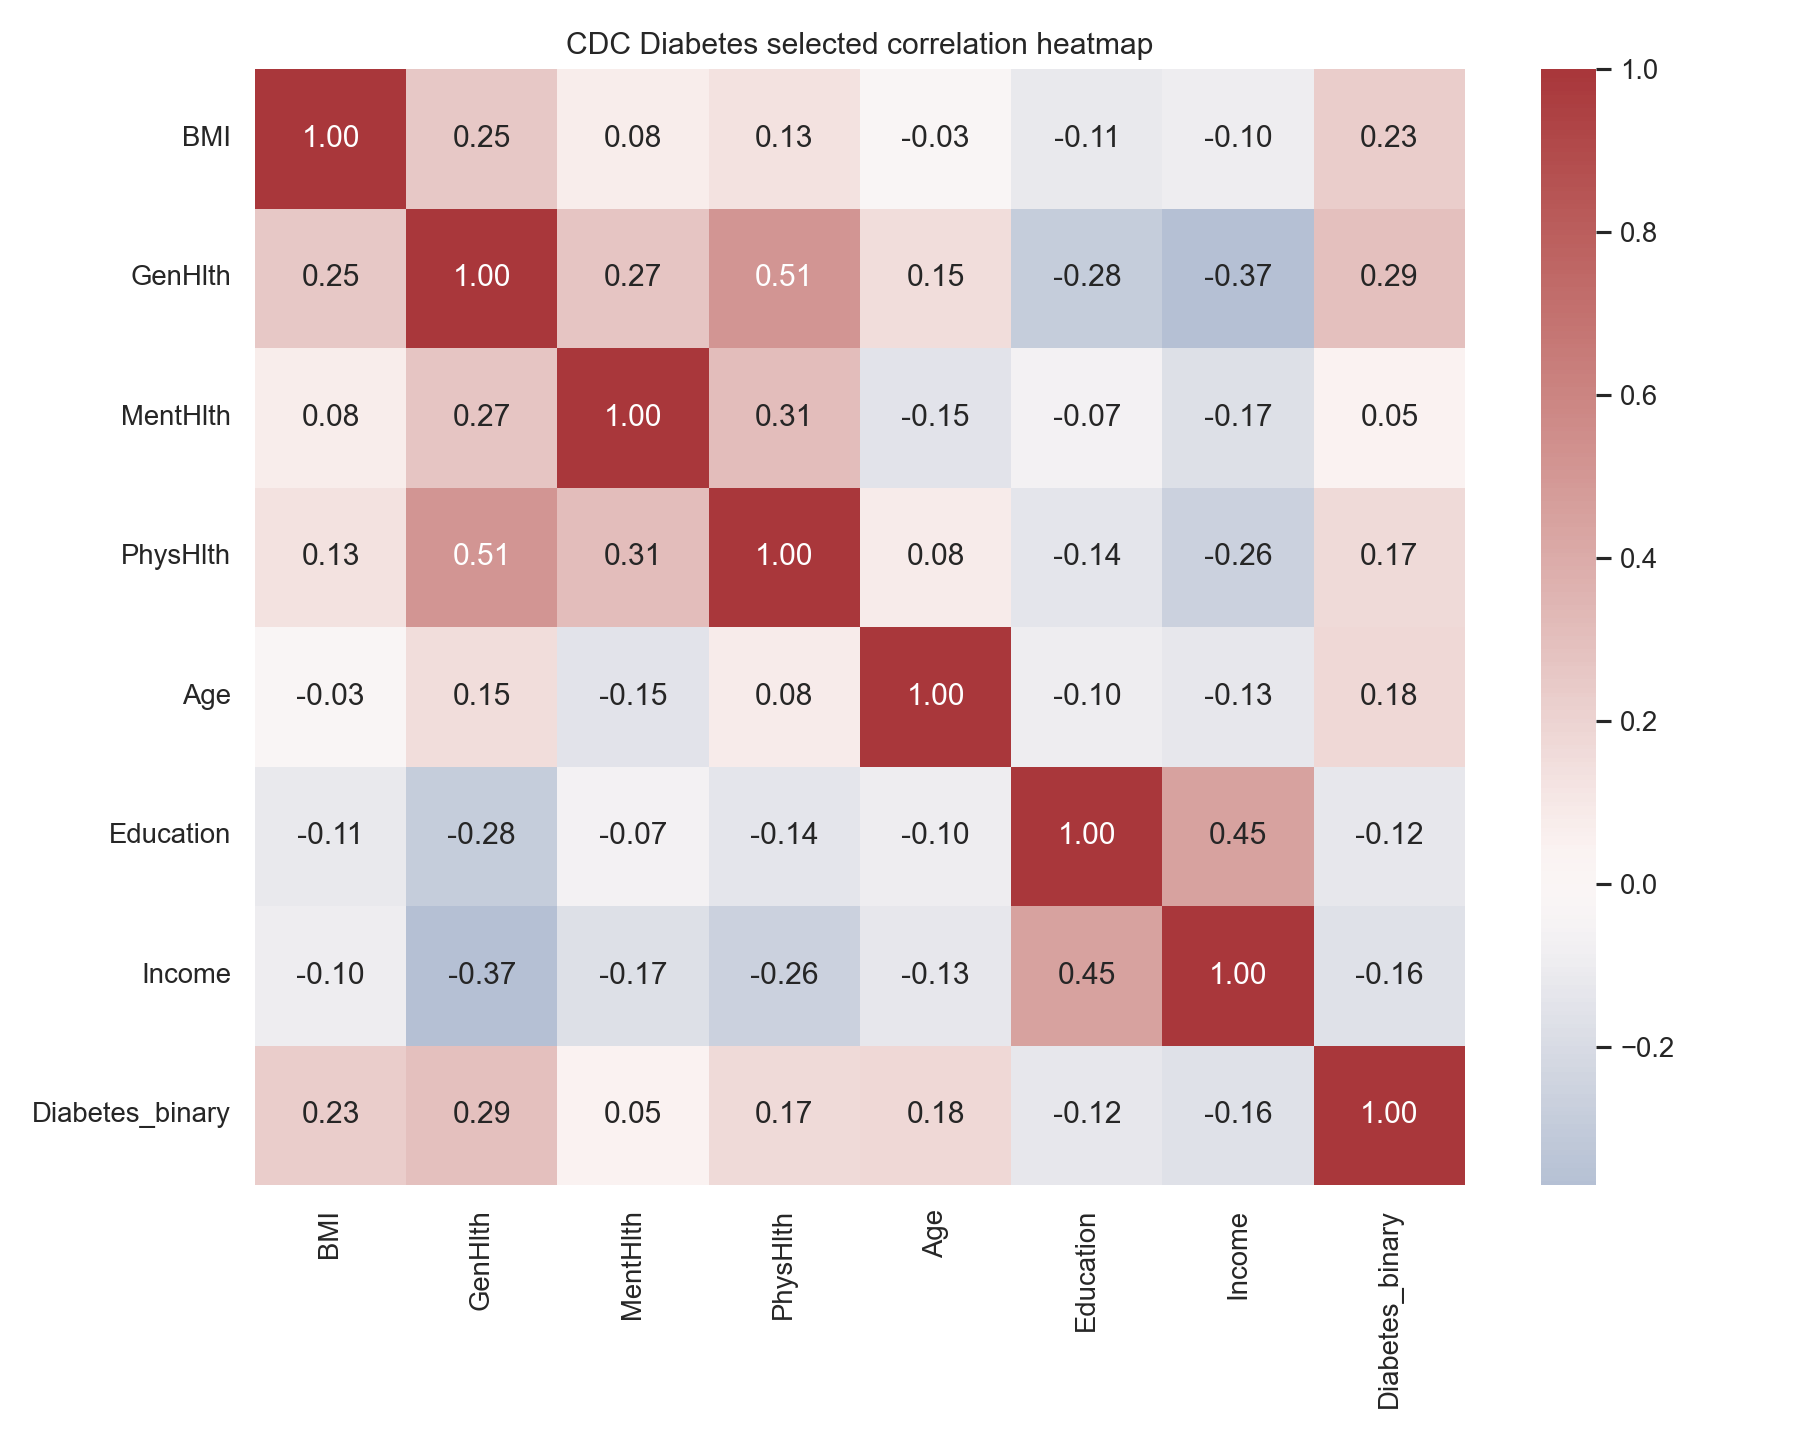
\includegraphics[width=0.86\textwidth]{images/ch3/cdc_diabetes_correlation_heatmap.png}
\captionsetup{justification=raggedright,singlelinecheck=false}
\caption[Heatmap tương quan CDC Diabetes]{Heatmap tương quan các biến CDC Diabetes.\\
\footnotesize Python source: \texttt{src/analyze\_cdc\_diabetes.py}.}
\label{fig:ch4_cdc_corr}
\end{figure}

\textbf{Nhận xét Hình \ref{fig:ch4_cdc_corr}.} Heatmap tương quan cho thấy nhóm \texttt{HighBP}, \texttt{HighChol}, \texttt{GenHlth} và \texttt{BMI} mô tả các khía cạnh khác nhau của nguy cơ chuyển hóa. Các tương quan không quá cao tuyệt đối, vì vậy từng biến vẫn có thể đóng góp thông tin riêng cho mô hình đa biến.

\textbf{Nhận xét về hình dáng phân phối.} \texttt{BMI}, \texttt{MentHlth} và \texttt{PhysHlth} đều lệch phải. Với \texttt{MentHlth} và \texttt{PhysHlth}, median và mode đều bằng 0 trong khi max đạt 30 ngày, cho thấy phần lớn người trả lời không ghi nhận ngày sức khỏe kém nhưng vẫn tồn tại một nhóm nhỏ có gánh nặng sức khỏe cao. Với \texttt{BMI}, mean lớn hơn median và đuôi phải dài, phản ánh một nhóm quan sát béo phì mức cao cần được kiểm soát bằng clipping trước khi mô hình hóa.

\textbf{Bước 4. So sánh trước--sau tiền xử lý.} Bảng~\ref{tab:ch4_cdc_preprocess} đặt các chỉ số của trạng thái thô cạnh trạng thái sạch; các hình thô/sạch ở trên minh họa trực tiếp tác động của clipping IQR.

\begin{table}[H]
\centering
\caption[So sánh dữ liệu thô và sạch CDC Diabetes]{Bước 4 -- So sánh dữ liệu thô và dữ liệu sạch CDC Diabetes (clipping IQR trên \texttt{BMI}, \texttt{MentHlth}, \texttt{PhysHlth}; 0 ô khuyết ở cả hai trạng thái). Source: \texttt{outputs/tables/cdc\_diabetes\_preprocessing\_comparison.csv}.}
\label{tab:ch4_cdc_preprocess}
\small
\begin{tabular}{lrrrrrr}
\toprule
Biến & Mean thô & Mean sạch & Std thô & Std sạch & Max thô & Max sạch \\
\midrule
\texttt{BMI} & 28.38 & 28.11 & 6.61 & 5.56 & 98.0 & 41.5 \\
\texttt{GenHlth} & 2.51 & 2.51 & 1.07 & 1.07 & 5.0 & 5.0 \\
\texttt{MentHlth} & 3.18 & 1.18 & 7.41 & 1.95 & 30.0 & 5.0 \\
\texttt{PhysHlth} & 4.24 & 1.85 & 8.72 & 2.89 & 30.0 & 7.5 \\
\texttt{Age} & 8.03 & 8.03 & 3.05 & 3.05 & 13.0 & 13.0 \\
\bottomrule
\end{tabular}
\end{table}

Bảng~\ref{tab:ch4_cdc_preprocess} cho thấy clipping IQR ảnh hưởng mạnh đến ba biến có ngoại lai và không làm thay đổi các biến ordinal đã sạch. Cụ thể, \texttt{BMI} giảm standard deviation 15.9\% (6.61$\to$5.56) và max giảm 57.7\% (98$\to$41.5); \texttt{MentHlth} giảm standard deviation 73.7\% (7.41$\to$1.95), còn \texttt{PhysHlth} giảm 66.9\% (8.72$\to$2.89). Trong khi đó, \texttt{GenHlth} và \texttt{Age} giữ nguyên mean, standard deviation và max vì các giá trị đã nằm trong miền hợp lệ.

\textbf{Kết luận cho CDC Diabetes.} Có ba kết quả chính rút ra từ phân tích. Thứ nhất, bộ dữ liệu không có ô khuyết, nên tiền xử lý tập trung vào ngoại lai thay vì điền khuyết. Thứ hai, clipping được áp dụng có chọn lọc cho \texttt{BMI}, \texttt{MentHlth} và \texttt{PhysHlth}, giúp giảm ảnh hưởng của đuôi phải cực trị nhưng vẫn giữ nguyên phần lõi phân phối. Thứ ba, biến mục tiêu mất cân bằng rõ rệt, do đó các phân tích và mô hình học máy cần ưu tiên metric theo lớp thay vì chỉ dựa vào accuracy.

\subsubsection{Breast Cancer Wisconsin Diagnostic}

Breast Cancer Wisconsin Diagnostic có 569 quan sát, 30 đặc trưng hình thái định lượng liên tục được trích xuất từ ảnh tế bào và biến mục tiêu \texttt{Diagnosis} gồm hai lớp B/M (lành tính/ác tính). Trong mục này, sáu biến đại diện được chọn là \texttt{radius1}, \texttt{texture1}, \texttt{perimeter1}, \texttt{area1}, \texttt{smoothness1} và \texttt{concavity1}. Nhóm biến này bao quát kích thước, bề mặt và độ lõm của khối u, do đó phù hợp để minh họa thống kê mô tả, trực quan hóa và đánh giá tác động của xử lý ngoại lai.

\textbf{Trạng thái dữ liệu thô.} Trước khi tính toán thống kê, dữ liệu được kiểm tra ô khuyết và giá trị ngoại lai. Breast Cancer \emph{không có ô khuyết thiếu} (0/569 dòng, theo \texttt{outputs/tables/breast\_cancer\_missing\_values.csv}), nên không cần điền khuyết. Đặc điểm cần chú ý là các đặc trưng hình thái có \emph{thang đo rất khác nhau}: \texttt{area1} có range xấp xỉ 2357, lớn hơn nhiều so với các biến như \texttt{smoothness1} hoặc \texttt{concavity1} có range nhỏ hơn 1.

\begin{figure}[H]
\centering
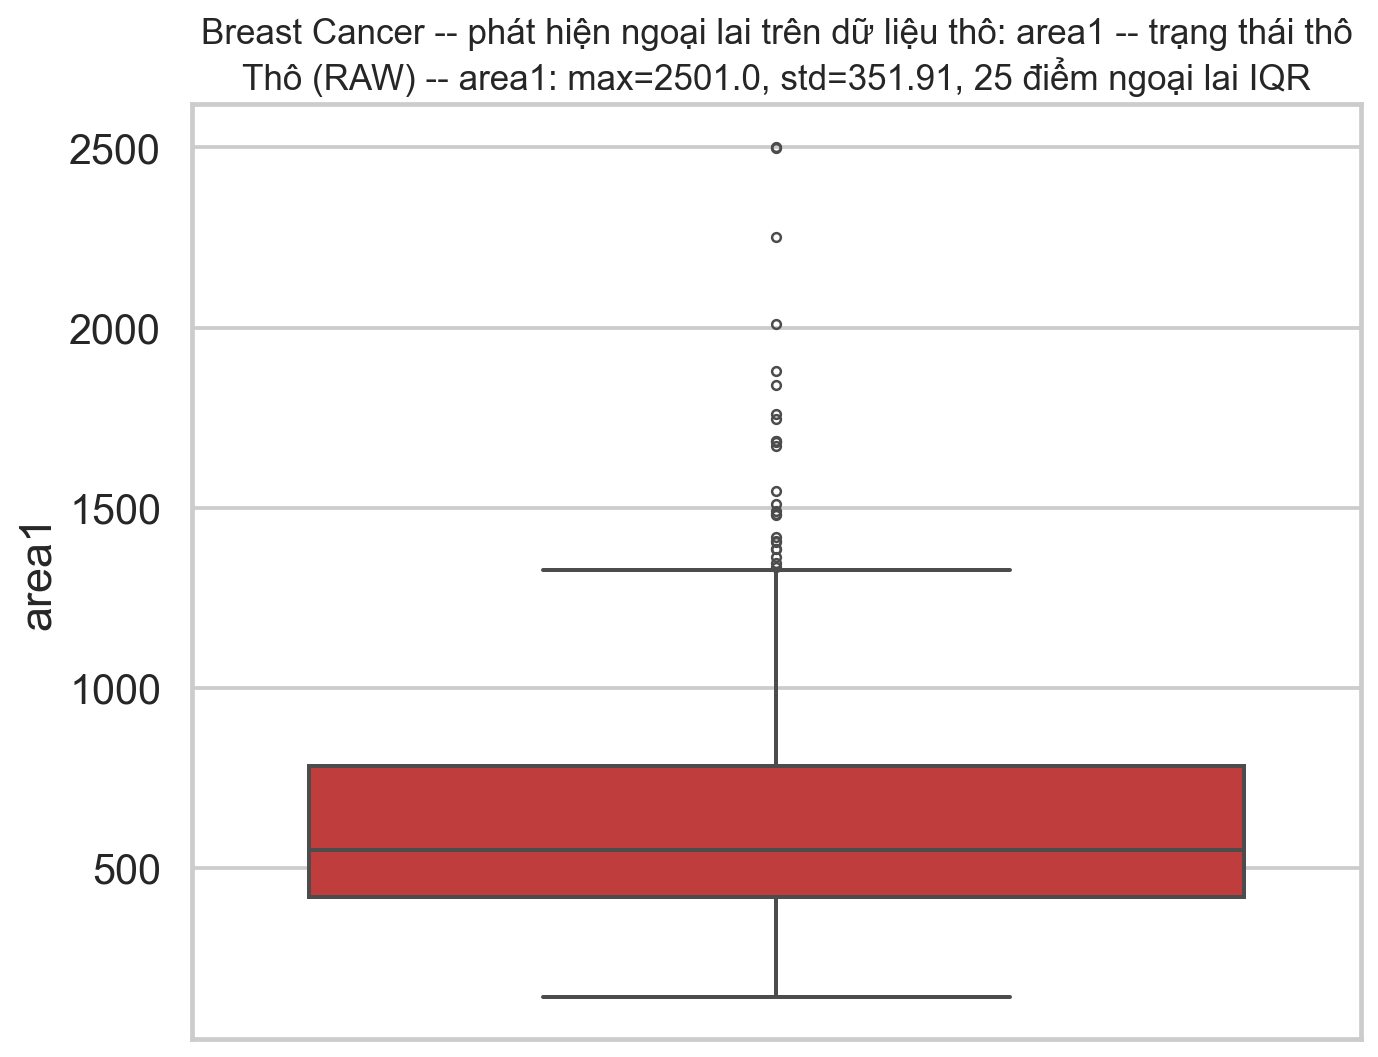
\includegraphics[width=0.72\textwidth]{images/ch3/breast_cancer_area1_boxplot_raw.png}
\captionsetup{justification=raggedright,singlelinecheck=false}
\caption[Boxplot \texttt{area1} thô Breast Cancer]{Boxplot \texttt{area1} Breast Cancer ở \textbf{trạng thái thô}: nhiều điểm ngoại lai tới $\sim$2501 (median 551), tập trung ở nhóm ác tính (M).\\
\footnotesize Python source: \texttt{scripts/generate\_raw\_vs\_cleaned\_boxplots.py}.}
\label{fig:ch4_breast_raw_boxplot}
\end{figure}

\textit{Phát hiện ngoại lai trên dữ liệu thô.} Hình~\ref{fig:ch4_breast_raw_boxplot} cho thấy một số ca khối u lớn tạo điểm rời rạc ở đuôi phải. \texttt{radius1} có các giá trị vượt 25 so với median 13.37; \texttt{perimeter1} đạt xấp xỉ 188; đặc biệt, \texttt{area1} đạt xấp xỉ 2501 trong khi median chỉ 551. Các điểm xa râu hộp này tập trung nhiều ở nhóm ác tính (M). Ngoài ra, \texttt{concavity1} lệch phải rõ với mode bằng 0 và một số ca đạt 0.427. Vì nhiều ngoại lai có thể phản ánh khối u ác tính kích thước lớn, clipping cần được áp dụng thận trọng thay vì loại bỏ cơ học.

\textbf{Làm sạch dữ liệu.} Quy trình tiền xử lý được thực hiện theo ba nguyên tắc sau:

\begin{itemize}[leftmargin=*]
    \item \textbf{Điền khuyết:} \emph{không cần} -- dữ liệu thô không có ô NaN.
    \item \textbf{Xử lý ngoại lai:} \emph{clipping theo quy tắc IQR} trên sáu biến được chọn \texttt{radius1}, \texttt{texture1}, \texttt{perimeter1}, \texttt{area1}, \texttt{smoothness1}, \texttt{concavity1}. Cách xử lý này nén giá trị cực trị về biên hộp nhưng vẫn giữ quan sát trong tập dữ liệu.
    \item \textbf{Chuẩn hóa:} \emph{chưa áp dụng} ở giai đoạn thống kê mô tả để giữ đơn vị hình thái gốc; Min--Max Scaling hoặc Z-score chỉ được dùng ở chương học máy khi cần đưa các đặc trưng về cùng thang đo.
\end{itemize}

\begin{figure}[H]
\centering
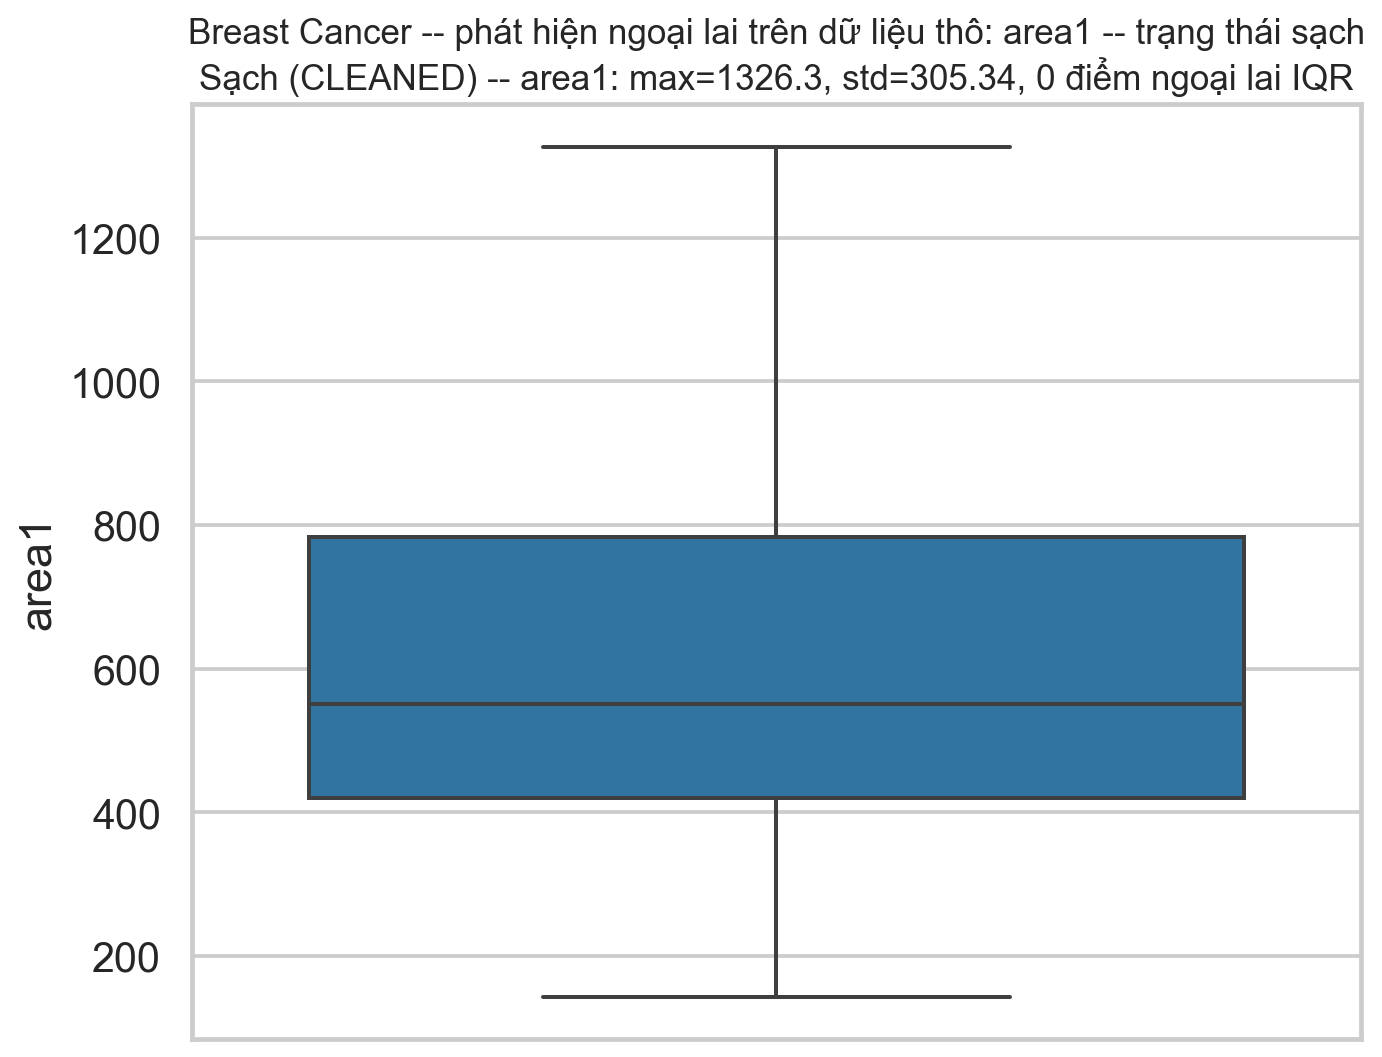
\includegraphics[width=0.72\textwidth]{images/ch3/breast_cancer_area1_boxplot_cleaned.png}
\captionsetup{justification=raggedright,singlelinecheck=false}
\caption[Boxplot \texttt{area1} sạch Breast Cancer]{Boxplot \texttt{area1} Breast Cancer ở \textbf{trạng thái sạch}: sau clipping IQR, các điểm ngoại lai được nén về ngưỡng trên hộp (max $\sim$2501 $\to$ $\sim$1326) nhưng vẫn giữ cấu trúc tách B/M.\\
\footnotesize Python source: \texttt{scripts/generate\_raw\_vs\_cleaned\_boxplots.py}.}
\label{fig:ch4_breast_cleaned_boxplot}
\end{figure}

\textbf{Bước 1. Phân loại bản chất biến.} Trước khi chọn thống kê và biểu đồ, các biến được phân loại theo bản chất đo lường. Với Breast Cancer, hầu hết đặc trưng đầu vào là Quantitative Continuous; riêng \texttt{Diagnosis} là biến Qualitative binary dùng để so sánh phân phối theo nhóm chẩn đoán.

\begin{table}[H]
\centering
\caption{Bước 1 -- Phân loại biến tiêu biểu trong Breast Cancer}
\label{tab:ch4_breast_variable_types}
\small
\begin{tabularx}{\textwidth}{p{0.18\textwidth}p{0.27\textwidth}p{0.25\textwidth}Y}
\toprule
Biến & Bản chất & Thống kê dùng & Biểu đồ phù hợp \\
\midrule
\texttt{Diagnosis} & Qualitative binary & Tần suất, mode & Bar chart \\
\texttt{radius1} & Quantitative Continuous & Mean, median, IQR & Histogram, boxplot \\
\texttt{texture1} & Quantitative Continuous & Mean, std, range & Histogram \\
\texttt{perimeter1} & Quantitative Continuous & Mean, median, IQR & Histogram, heatmap \\
\texttt{area1} & Quantitative Continuous & Range, variance, CV & Histogram, boxplot \\
\texttt{smoothness1} & Quantitative Continuous & Mean, median, IQR & Histogram, boxplot \\
\texttt{concavity1} & Quantitative Continuous & CV, skewness proxy & Histogram, boxplot \\
\bottomrule
\end{tabularx}
\end{table}

\textbf{Bước 2. Bảng tần suất và thống kê mô tả.} Biến \texttt{Diagnosis} được mô tả bằng tần suất tuyệt đối, tần suất tương đối và mode. Các biến hình thái định lượng được mô tả bằng mean, median, mode, percentile, range, variance, standard deviation, CV và IQR.

\begin{table}[H]
\centering
\caption[Bảng tần suất \texttt{Diagnosis} trong Breast Cancer]{Bước 2 -- Bảng tần suất biến \texttt{Diagnosis} trong Breast Cancer. Source: \texttt{outputs/tables/breast\_cancer\_frequency\_Diagnosis.csv}.}
\label{tab:ch4_breast_frequency}
\small
\begin{tabular}{lrr}
\toprule
\texttt{Diagnosis} & Tần suất tuyệt đối & Tần suất tương đối \\
\midrule
B (lành tính) & 357 & 62.74\% \\
M (ác tính) & 212 & 37.26\% \\
\bottomrule
\end{tabular}
\end{table}

\begin{table}[H]
\centering
\caption[Thống kê mô tả Breast Cancer]{Thống kê mô tả Breast Cancer: xu hướng trung tâm và độ phân tán. Source: \texttt{outputs/tables/breast\_cancer\_summary.csv}.}
\label{tab:ch4_breast_stats}
\scriptsize
\setlength{\tabcolsep}{3pt}
\begin{tabular}{lrrrrrrrrrr}
\toprule
Biến & Mean & Med & Mode & P25 & P75 & Range & Var & Std & CV & IQR \\
\midrule
\texttt{radius1} & 14.13 & 13.37 & 12.34 & 11.70 & 15.78 & 21.13 & 12.42 & 3.52 & 0.249 & 4.08 \\
\texttt{texture1} & 19.29 & 18.84 & 14.93 & 16.17 & 21.80 & 29.57 & 18.50 & 4.30 & 0.223 & 5.63 \\
\texttt{perimeter1} & 91.97 & 86.24 & 82.61 & 75.17 & 104.10 & 144.71 & 590.44 & 24.30 & 0.264 & 28.93 \\
\texttt{area1} & 654.89 & 551.10 & 512.20 & 420.30 & 782.70 & 2357.50 & 123843.6 & 351.91 & 0.537 & 362.40 \\
\texttt{smoothness1} & 0.096 & 0.096 & 0.101 & 0.086 & 0.105 & 0.111 & 0.0002 & 0.014 & 0.146 & 0.019 \\
\texttt{concavity1} & 0.089 & 0.062 & 0.000 & 0.030 & 0.131 & 0.427 & 0.006 & 0.080 & 0.898 & 0.101 \\
\bottomrule
\end{tabular}
\end{table}

\begin{table}[H]
\centering
\caption[Thống kê thô/sạch Breast Cancer]{So sánh thống kê mô tả Breast Cancer ở hai trạng thái: \textbf{thô} và \textbf{sạch} (clipping IQR trên 6 biến hình thái). Source: \texttt{outputs/tables/breast\_cancer\_summary.csv}.}
\label{tab:ch4_breast_stats_raw_clean}
\footnotesize
\setlength{\tabcolsep}{4pt}
\begin{tabular}{lcrrrrrr}
\toprule
Biến & Trạng thái & Mean & Median & Std & \textbf{Max} & \textbf{Range} & IQR \\
\midrule
\texttt{radius1} & thô & 14.13 & 13.37 & 3.52 & \textbf{28.11} & 21.13 & 4.08 \\
 & sạch & 14.06 & 13.37 & 3.34 & \textbf{21.90} & 14.92 & 4.08 \\
\midrule
\texttt{texture1} & thô & 19.29 & 18.84 & 4.30 & 39.28 & 29.57 & 5.63 \\
 & sạch & 19.25 & 18.84 & 4.19 & 30.24 & 20.54 & 5.63 \\
\midrule
\texttt{perimeter1} & thô & 91.97 & 86.24 & 24.30 & 188.50 & 144.71 & 28.93 \\
 & sạch & 91.54 & 86.24 & 23.05 & 147.50 & 103.70 & 28.93 \\
\midrule
\texttt{area1} & thô & 654.89 & 551.10 & 351.91 & \textbf{2501.00} & 2357.50 & 362.40 \\
 & sạch & 639.77 & 551.10 & 305.34 & \textbf{1326.30} & 1182.80 & 362.40 \\
\midrule
\texttt{smoothness1} & thô & 0.096 & 0.096 & 0.014 & 0.163 & 0.111 & 0.019 \\
 & sạch & 0.096 & 0.096 & 0.014 & 0.134 & 0.076 & 0.019 \\
\midrule
\texttt{concavity1} & thô & 0.089 & 0.062 & 0.080 & 0.427 & 0.427 & 0.101 \\
 & sạch & 0.087 & 0.062 & 0.074 & 0.282 & 0.282 & 0.101 \\
\bottomrule
\end{tabular}
\end{table}

\textit{Nhận xét thô/sạch.} \texttt{area1} là biến có thang đo lớn nhất và cũng giảm max mạnh nhất sau clipping: từ 2501 xuống 1326, đồng thời standard deviation giảm từ 351.91 xuống 305.34. \texttt{radius1} giảm max từ 28.11 xuống 21.90. Đáng chú ý, median và IQR của các biến đều không đổi, cho thấy clipping chỉ nén phần đuôi mà không dịch chuyển vùng trung tâm của phân phối. Đây là điều quan trọng vì tín hiệu phân biệt khối u lành/ác chủ yếu nằm ở sự tách biệt trung tâm và khoảng tứ phân vị giữa hai nhóm.

\textbf{Bước 3. Trực quan hóa dữ liệu.} Hệ thống biểu đồ được lựa chọn theo cùng cấu trúc với Heart Disease: bar chart cho phân bố \texttt{Diagnosis}, histogram cho \texttt{radius1}, boxplot theo target để đọc khả năng phân tách B/M, scatter plot cho quan hệ hai đặc trưng, đối chiếu thô/sạch để đánh giá clipping và heatmap để khảo sát tương quan giữa các biến hình thái.

\begin{figure}[H]
\centering
\begin{subfigure}{0.90\textwidth}
 \centering
 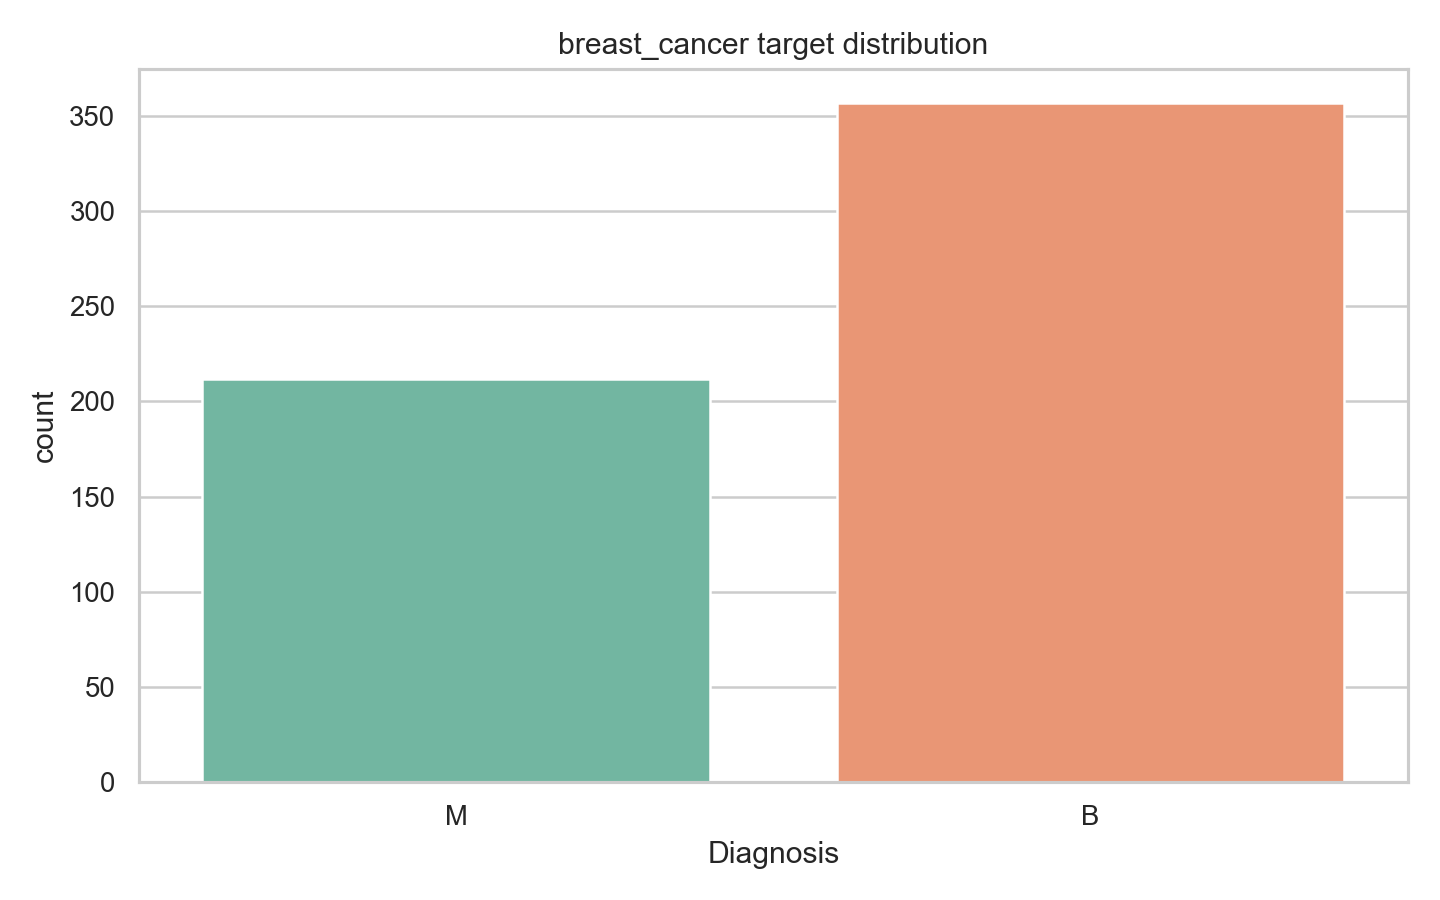
\includegraphics[width=\textwidth]{images/ch3/breast_cancer_target_distribution.png}
 \caption{Python -- Phân bố \texttt{Diagnosis}}
\end{subfigure}
\par\medskip
\begin{subfigure}{0.90\textwidth}
 \centering
 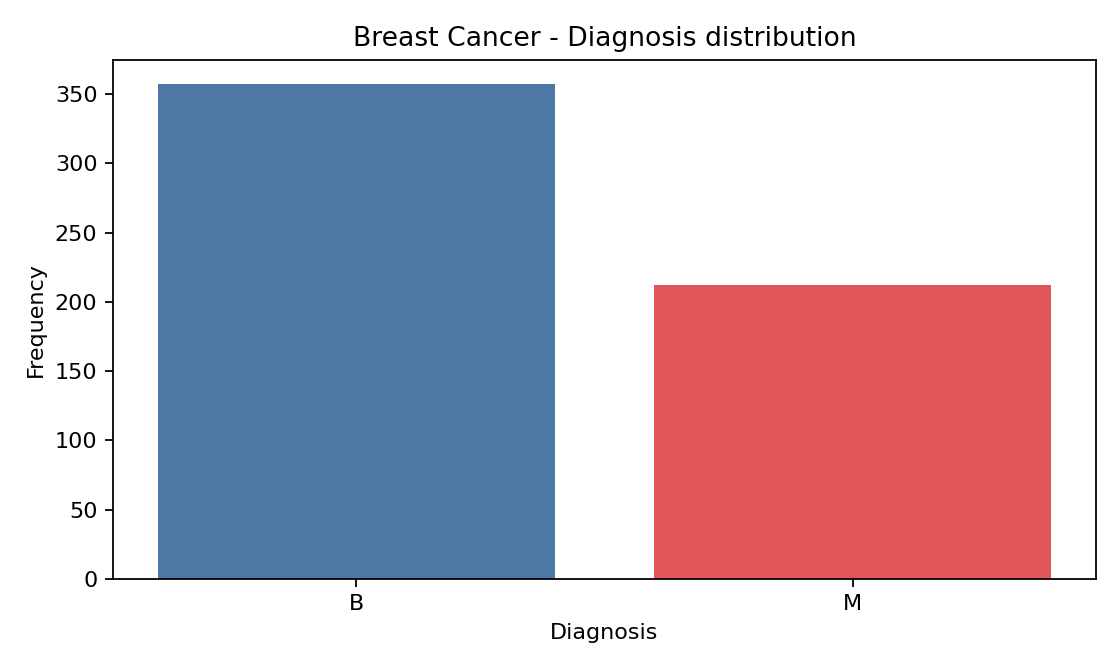
\includegraphics[width=\textwidth]{images/ch3/excel_breast_target_distribution_preview.png}
 \caption{Excel -- Phân bố \texttt{Diagnosis}}
\end{subfigure}
\captionsetup{justification=raggedright,singlelinecheck=false}
\caption[Phân bố target Breast Cancer: Python và Excel]{Phân bố \texttt{Diagnosis} trong Breast Cancer, đối chiếu giữa Python và Excel.\\
\footnotesize Python source: \texttt{src/analyze\_tabular\_health.py}.\\
Excel source/workbook: \texttt{src/create\_excel\_visualizations.py}, \texttt{excel/excel\_visualization\_comparison\_native.xlsx}, sheet \texttt{Breast Target}.}
\label{fig:ch4_breast_target}
\end{figure}

\textbf{Nhận xét Hình \ref{fig:ch4_breast_target}.} Lớp B chiếm 62.74\%, lớp M chiếm 37.26\%; dữ liệu không cân bằng nhẹ nhưng không quá cực đoan.

\begin{figure}[H]
\centering
\begin{subfigure}{0.90\textwidth}
 \centering
 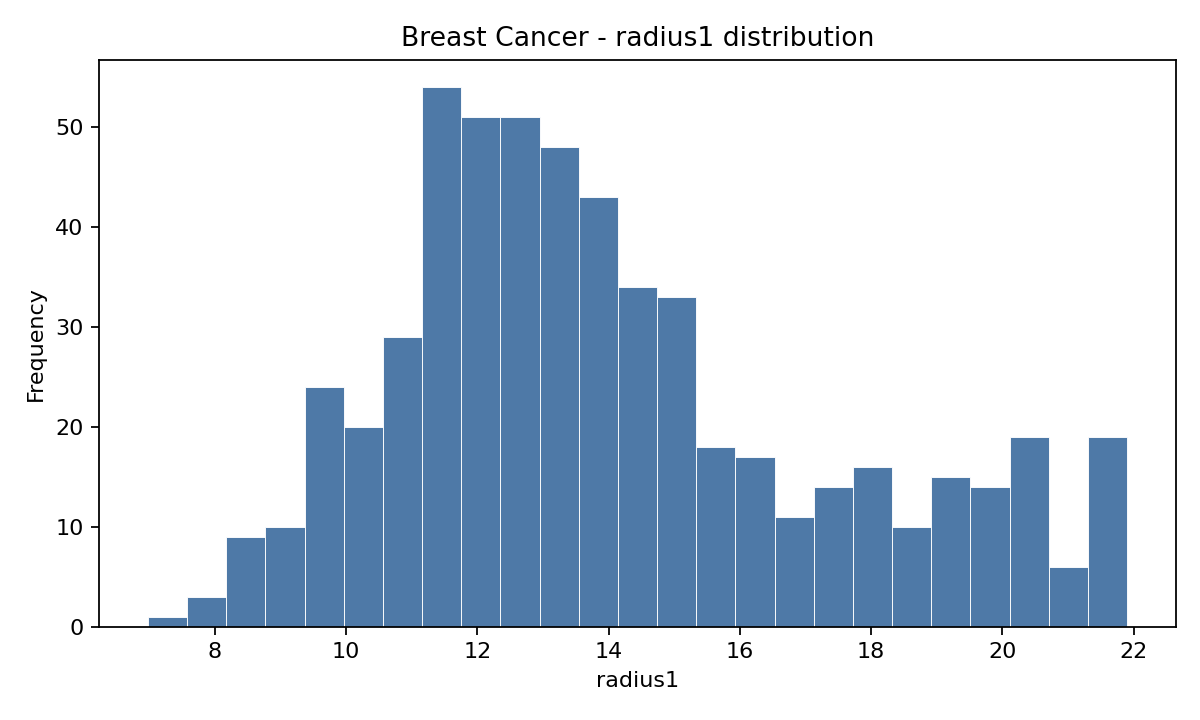
\includegraphics[width=\textwidth]{images/ch3/breast_cancer_radius1_hist.png}
 \caption{Python -- Histogram \texttt{radius1}}
\end{subfigure}
\par\medskip
\begin{subfigure}{0.90\textwidth}
 \centering
 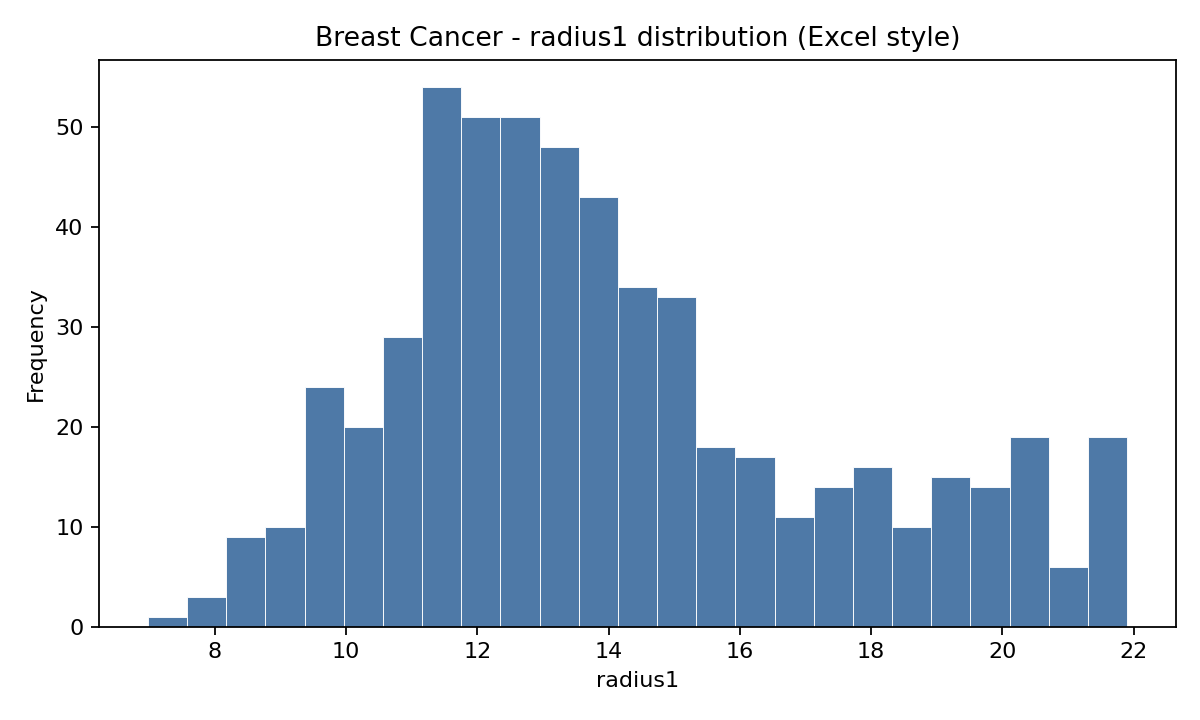
\includegraphics[width=\textwidth]{images/ch3/excel_breast_radius_hist_preview.png}
 \caption{Excel -- Histogram \texttt{radius1}}
\end{subfigure}
\captionsetup{justification=raggedright,singlelinecheck=false}
\caption[Histogram \texttt{radius1} Breast Cancer: Python và Excel]{Phân phối \texttt{radius1} trong Breast Cancer, đối chiếu giữa Python và Excel.\\
\footnotesize Python source: \texttt{src/analyze\_tabular\_health.py}.\\
Excel source/workbook: \texttt{src/create\_excel\_visualizations.py}, \texttt{excel/excel\_visualization\_comparison\_native.xlsx}, sheet \texttt{Breast Radius Hist}.}
\label{fig:ch4_breast_radius_hist}
\end{figure}

\textbf{Nhận xét Hình \ref{fig:ch4_breast_radius_hist}.} \texttt{radius1} lệch phải nhẹ: mean 14.13 lớn hơn median 13.37.

\begin{figure}[H]
\centering
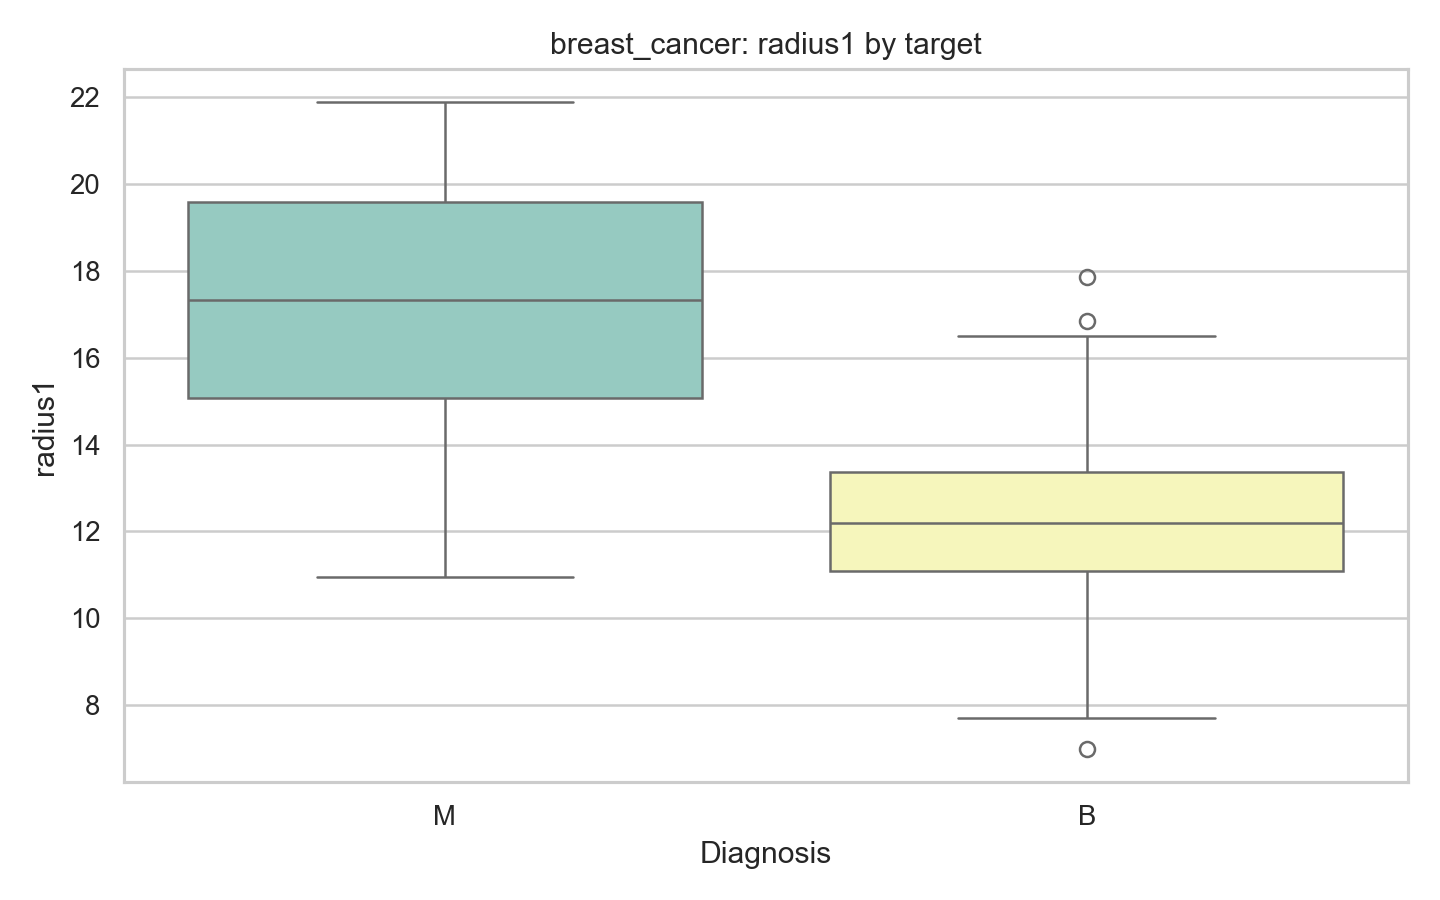
\includegraphics[width=0.90\textwidth]{images/ch3/breast_cancer_radius1_boxplot_by_target.png}
\captionsetup{justification=raggedright,singlelinecheck=false}
\caption[Boxplot \texttt{radius1} Breast Cancer]{Boxplot \texttt{radius1} theo chẩn đoán B/M.\\
\footnotesize Python source: \texttt{src/analyze\_tabular\_health.py}.}
\label{fig:ch4_breast_radius_boxplot}
\end{figure}

\textbf{Nhận xét Hình \ref{fig:ch4_breast_radius_boxplot}.} Nhóm ác tính (M) có trung vị và khoảng phân vị \texttt{radius1} cao hơn nhóm lành tính (B), hai hộp tách khá rõ.

\begin{figure}[H]
\centering
\begin{subfigure}{0.90\textwidth}
 \centering
 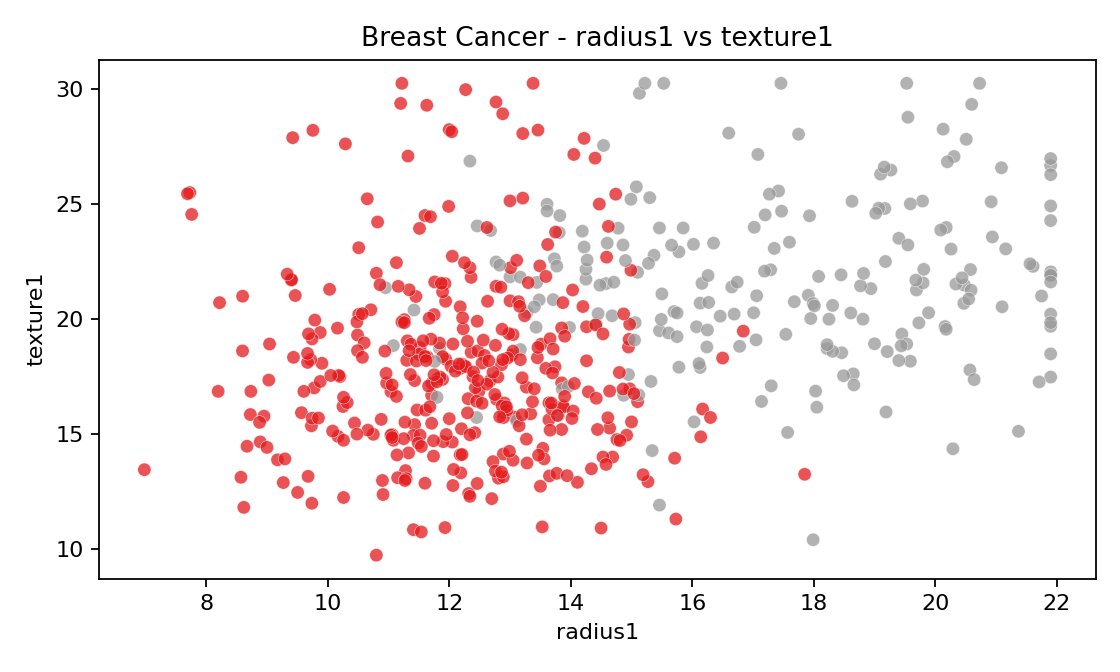
\includegraphics[width=\textwidth]{images/ch3/breast_cancer_radius_texture_scatter.png}
 \caption{Python -- Scatter \texttt{radius1}--\texttt{texture1}}
\end{subfigure}
\par\medskip
\begin{subfigure}{0.90\textwidth}
 \centering
 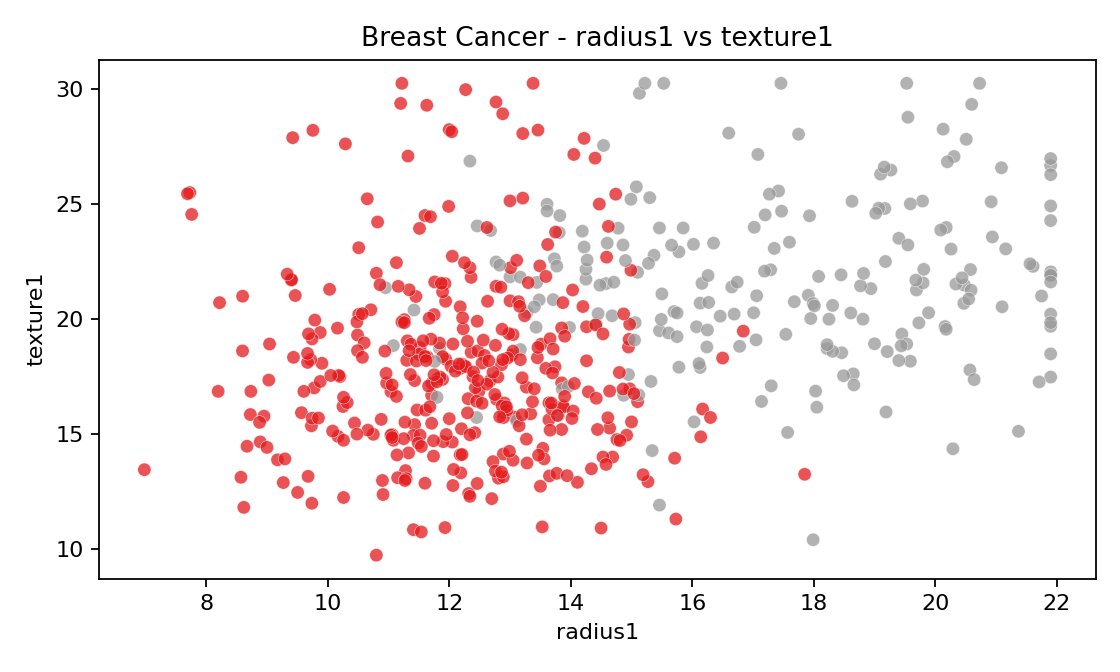
\includegraphics[width=\textwidth]{images/ch3/excel_breast_radius_texture_scatter_preview.png}
 \caption{Excel -- Scatter \texttt{radius1}--\texttt{texture1}}
\end{subfigure}
\captionsetup{justification=raggedright,singlelinecheck=false}
\caption[Scatter Breast Cancer: Python và Excel]{Scatter giữa \texttt{radius1} và \texttt{texture1}, đối chiếu giữa Python và Excel.\\
\footnotesize Python source: \texttt{src/analyze\_tabular\_health.py}.\\
Excel source/workbook: \texttt{src/create\_excel\_visualizations.py}, \texttt{excel/excel\_visualization\_comparison\_native.xlsx}, sheet \texttt{Breast Scatter}.}
\label{fig:ch4_breast_scatter}
\end{figure}

\textbf{Nhận xét Hình \ref{fig:ch4_breast_scatter}.} Nhóm M thường dịch về vùng \texttt{radius1} lớn hơn, còn \texttt{texture1} bổ sung độ tách theo chiều thứ hai.

\textit{Đối chiếu thô/sạch.} Ba biểu đồ tiếp theo đặt dữ liệu thô (đỏ) cạnh dữ liệu sạch (xanh), qua đó thể hiện trực quan tác động của clipping IQR trên các biến hình thái.

\begin{figure}[H]
\centering
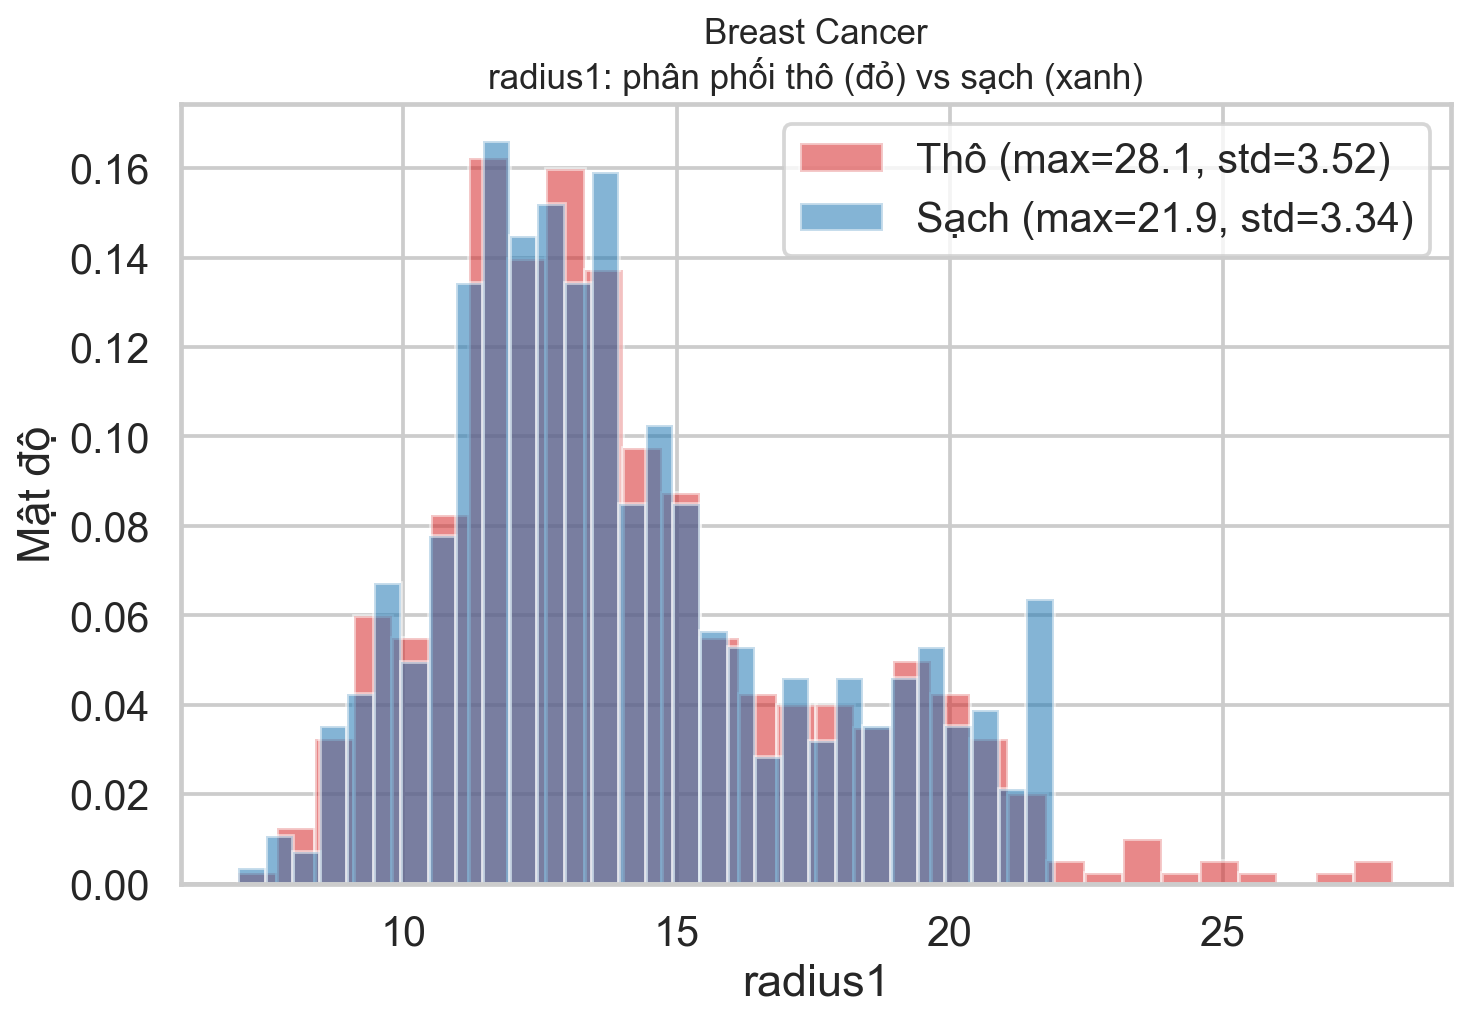
\includegraphics[width=0.82\textwidth]{images/ch3/breast_cancer_radius1_hist_raw_vs_cleaned.png}
\captionsetup{justification=raggedright,singlelinecheck=false}
\caption[Histogram \texttt{radius1} thô/sạch Breast Cancer]{Histogram \texttt{radius1} Breast Cancer: dữ liệu thô (đỏ, đuôi phải tới $\sim$28) chồng lên dữ liệu sạch (xanh, đuôi nén về $\sim$21.9).\\
\footnotesize Python source: \texttt{scripts/generate\_raw\_vs\_cleaned\_boxplots.py}.}
\label{fig:ch4_breast_hist_compare}
\end{figure}

\begin{figure}[H]
\centering
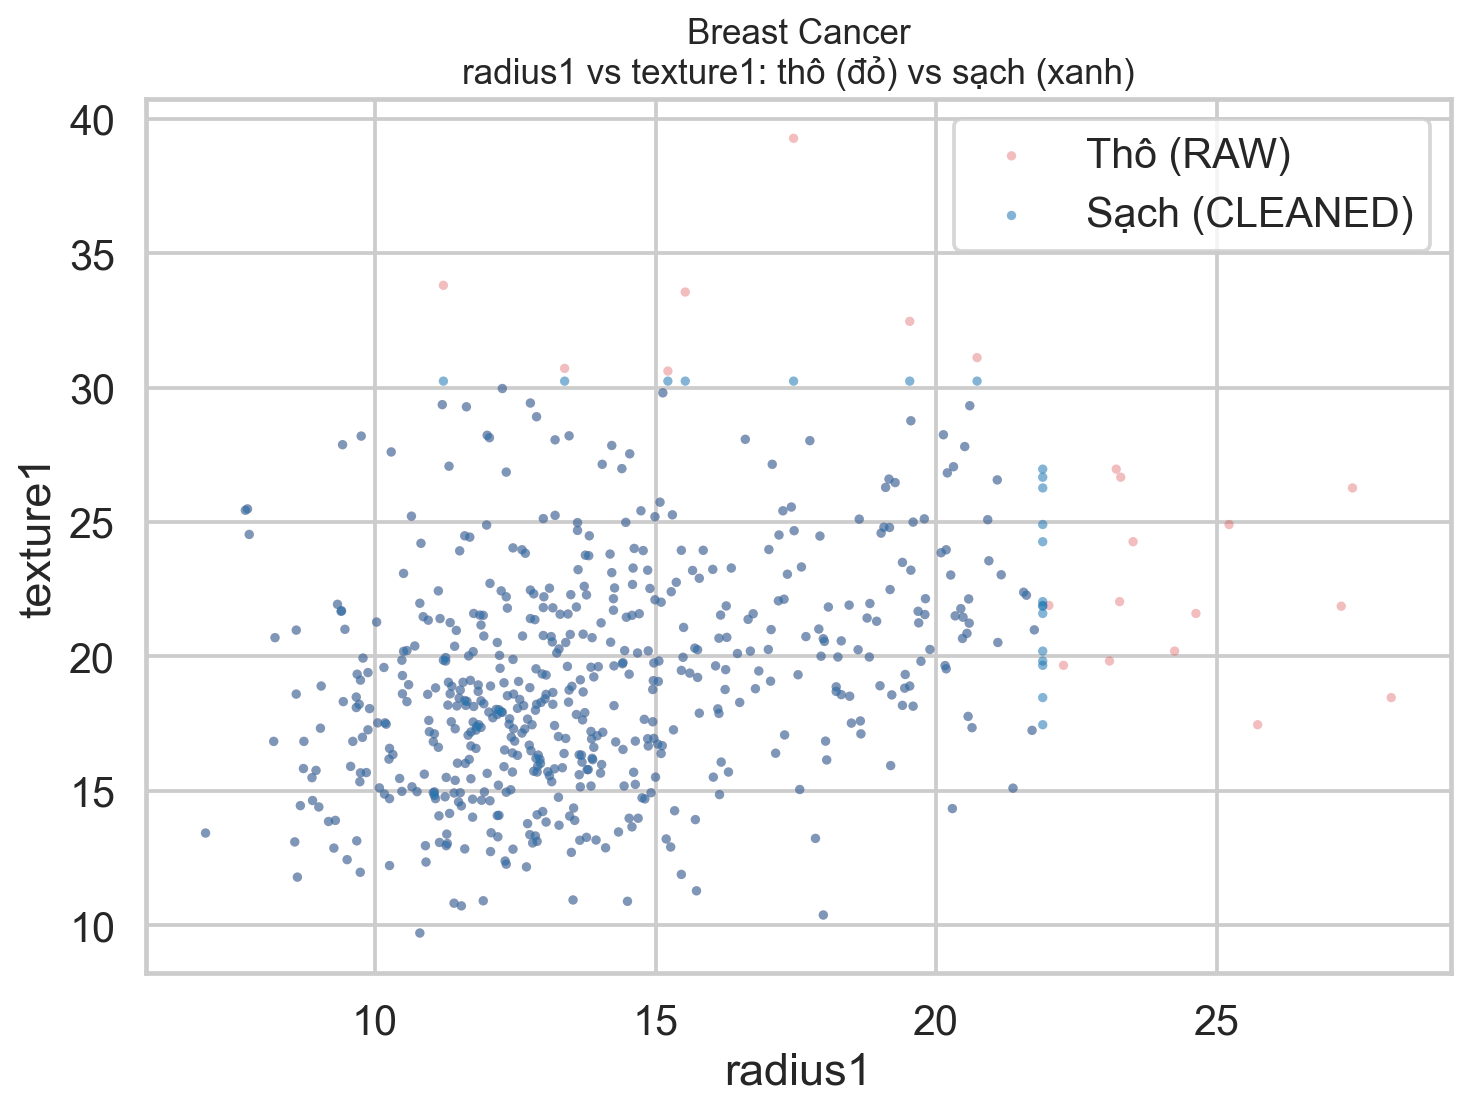
\includegraphics[width=0.82\textwidth]{images/ch3/breast_cancer_radius_texture_scatter_raw_vs_cleaned.png}
\captionsetup{justification=raggedright,singlelinecheck=false}
\caption[Scatter \texttt{radius1}--\texttt{texture1} thô/sạch Breast Cancer]{Scatter \texttt{radius1}--\texttt{texture1} Breast Cancer: dữ liệu thô (đỏ, mờ) phủ tới radius1$\sim$28; dữ liệu sạch (xanh) bị nén nhưng vùng M (bên phải) vẫn tách rõ.\\
\footnotesize Python source: \texttt{scripts/generate\_raw\_vs\_cleaned\_boxplots.py}.}
\label{fig:ch4_breast_scatter_compare}
\end{figure}

\begin{figure}[H]
\centering
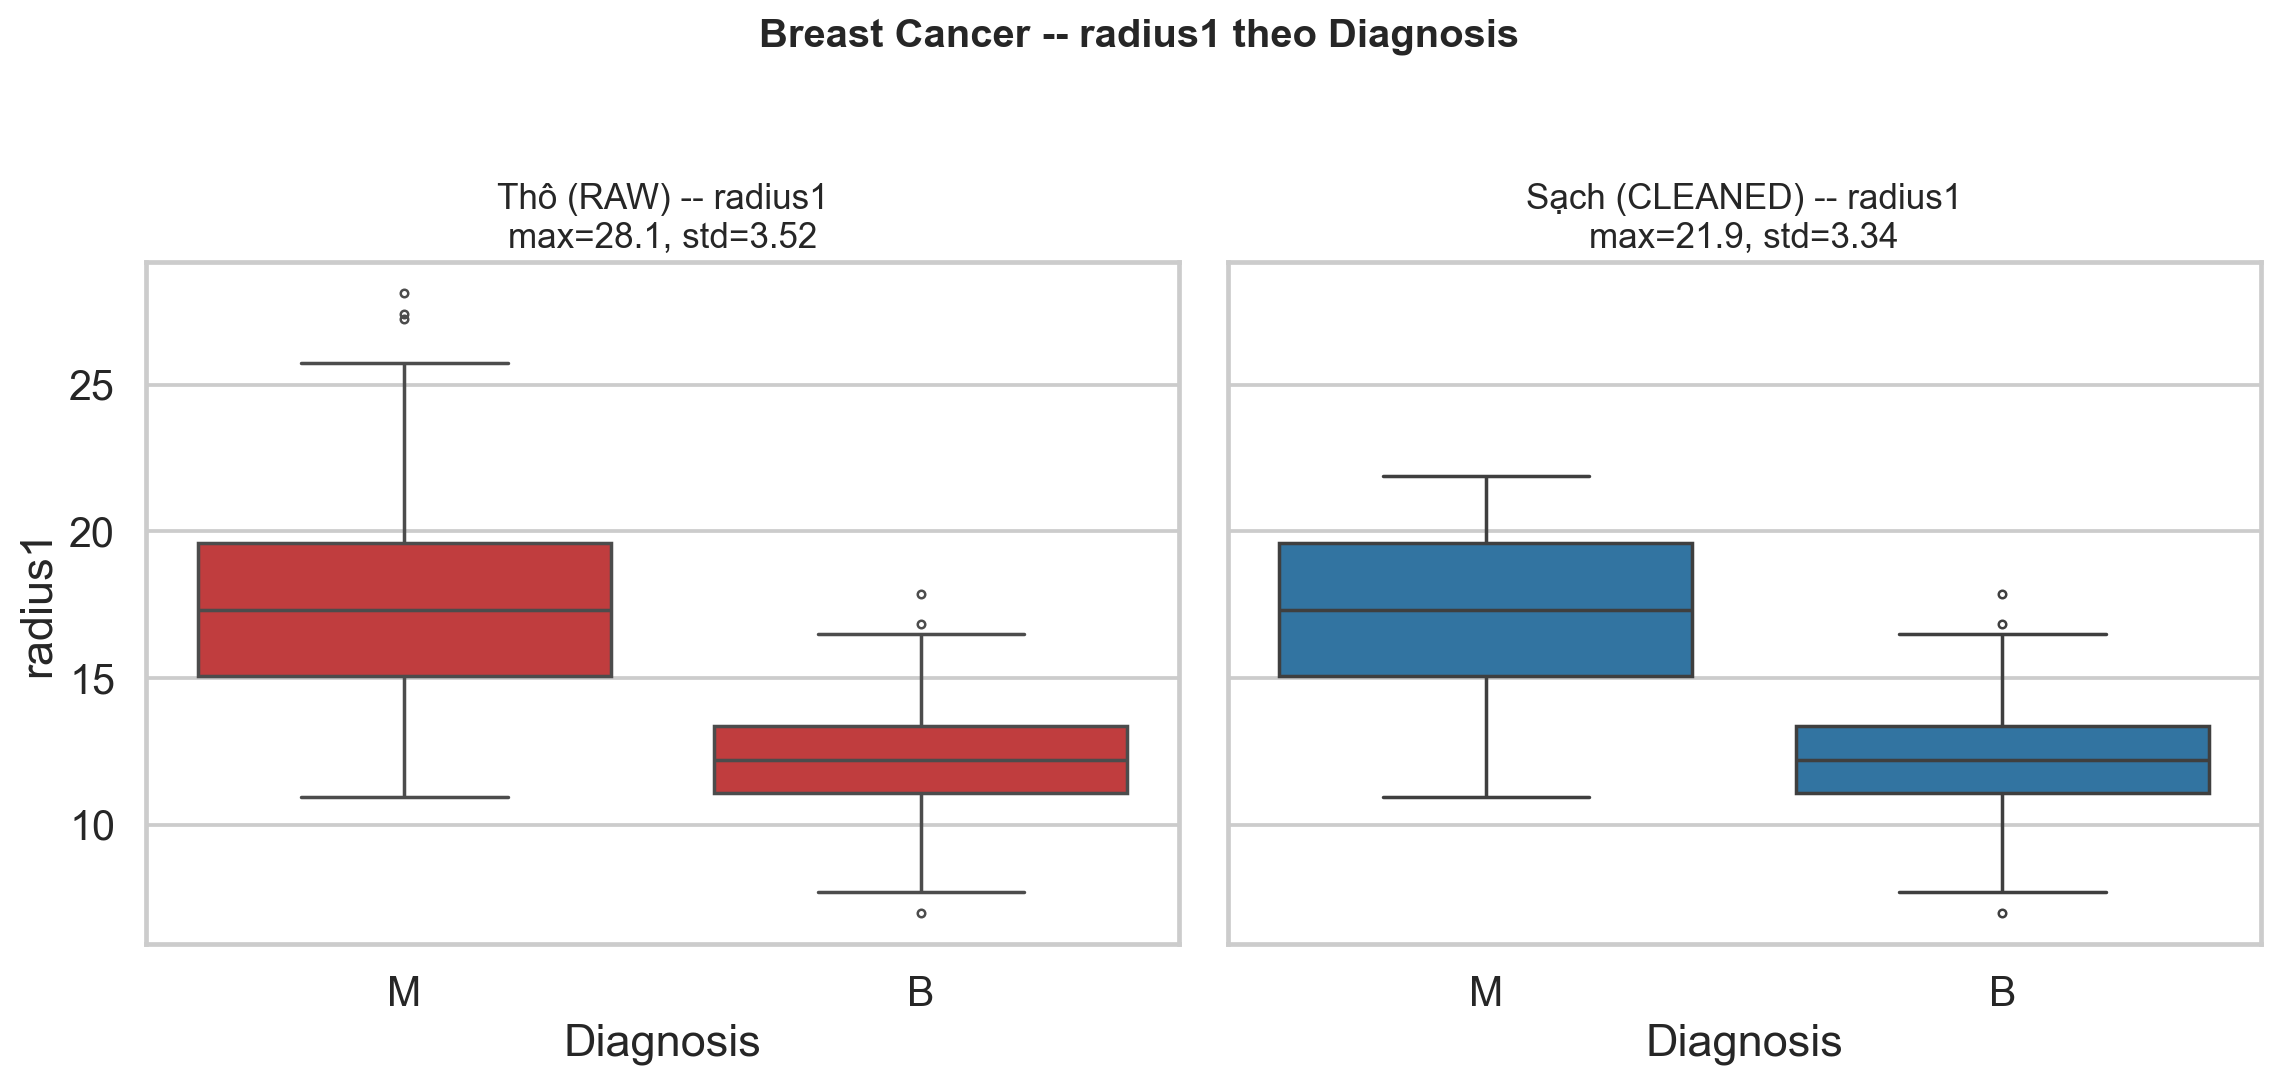
\includegraphics[width=0.95\textwidth]{images/ch3/breast_cancer_radius1_boxplot_by_target_raw_vs_cleaned.png}
\captionsetup{justification=raggedright,singlelinecheck=false}
\caption[Boxplot \texttt{radius1} theo Diagnosis thô/sạch Breast Cancer]{Boxplot \texttt{radius1} theo \texttt{Diagnosis}: thô (trái) có nhiều điểm ngoại lai; sạch (phải) giảm ngoại lai nhưng trung vị nhóm M vẫn cao hơn B rõ rệt.\\
\footnotesize Python source: \texttt{scripts/generate\_raw\_vs\_cleaned\_boxplots.py}.}
\label{fig:ch4_breast_boxplot_by_target_compare}
\end{figure}

\textbf{Nhận xét.} Histogram \texttt{radius1} (Hình~\ref{fig:ch4_breast_hist_compare}) cho thấy đuôi phải dữ liệu thô tới $\sim$28 bị nén về $\sim$21.9 ở dữ liệu sạch, phần lõi vẫn trùng nhau. Scatter (Hình~\ref{fig:ch4_breast_scatter_compare}) xác nhận vùng cao của \texttt{radius1} (đỏ) bị cắt nhưng cụm nhóm M (bên phải) vẫn giữ vị trí tương đối. Boxplot theo Diagnosis (Hình~\ref{fig:ch4_breast_boxplot_by_target_compare}) cho thấy sau clipping số điểm ngoài râu giảm, nhưng hai hộp B/M vẫn tách rõ -- clipping giảm nhiễu mà không phá tín hiệu chẩn đoán.

\begin{figure}[H]
\centering
\includegraphics[width=0.86\textwidth]{images/ch3/breast_cancer_correlation_heatmap.png}
\captionsetup{justification=raggedright,singlelinecheck=false}
\caption[Heatmap tương quan Breast Cancer]{Heatmap tương quan các đặc trưng hình thái Breast Cancer.\\
\footnotesize Python source: \texttt{src/analyze\_tabular\_health.py}.}
\label{fig:ch4_breast_corr}
\end{figure}

\textbf{Nhận xét Hình \ref{fig:ch4_breast_corr}.} Nhóm biến kích thước như \texttt{radius1}, \texttt{perimeter1} và \texttt{area1} tương quan rất mạnh, phản ánh chúng cùng đo quy mô khối u từ các góc nhìn khác nhau. Khi đưa vào mô hình tuyến tính, cần chú ý đa cộng tuyến; với các mô hình cây, nhóm biến này vẫn có thể hỗ trợ phân tách lớp hiệu quả.

\textbf{Nhận xét về hình dáng phân phối.} Các biến kích thước khối u như \texttt{radius1}, \texttt{perimeter1} và \texttt{area1} đều có mean lớn hơn median, cho thấy phân phối lệch phải. Điều này phù hợp với thực tế dữ liệu: phần lớn khối u tập trung ở kích thước trung bình hoặc nhỏ, trong khi một số ca ác tính có kích thước lớn tạo đuôi phải. \texttt{concavity1} lệch phải mạnh hơn, với mode bằng 0, phản ánh nhiều quan sát có độ lõm thấp nhưng vẫn tồn tại một nhóm nhỏ có độ lõm cao.

\textbf{Bước 4. So sánh trước--sau tiền xử lý.} Bảng~\ref{tab:ch4_breast_stats_raw_clean} đặt các chỉ số của trạng thái thô cạnh trạng thái sạch; các hình thô/sạch ở trên minh họa trực tiếp tác động của clipping IQR.

Bảng~\ref{tab:ch4_breast_stats_raw_clean} cho thấy sự khác biệt giữa thô và sạch hoàn toàn đến từ xử lý ngoại lai, vì bộ dữ liệu không có ô khuyết. Trên dữ liệu thô, \texttt{radius1} có các ca cực trị vượt 25 và \texttt{area1} có range xấp xỉ 2357; sau clipping IQR, các đỉnh này được nén về biên hộp, làm standard deviation và range giảm. Tuy nhiên, trung vị và IQR vẫn ổn định, đồng thời boxplot theo chẩn đoán (Hình~\ref{fig:ch4_breast_boxplot_by_target_compare}) cho thấy nhóm M vẫn có trung vị \texttt{radius1} cao hơn nhóm B. Như vậy, tiền xử lý làm giảm ảnh hưởng của cực trị nhưng không làm mất tín hiệu phân loại chẩn đoán.

\textbf{Kết luận cho Breast Cancer.} Có ba kết quả chính rút ra từ phân tích. Thứ nhất, dữ liệu không có ô khuyết, nên bước chuẩn bị tập trung vào kiểm soát ngoại lai và giữ đơn vị đo gốc để diễn giải hình thái khối u. Thứ hai, clipping IQR làm giảm đuôi phải của các biến kích thước, đặc biệt \texttt{area1} và \texttt{radius1}, nhưng không làm thay đổi median/IQR. Thứ ba, tín hiệu phân biệt giữa B và M vẫn rõ sau tiền xử lý, thể hiện qua boxplot và scatter plot; vì vậy dữ liệu sạch phù hợp hơn cho mô hình học máy mà vẫn bảo toàn ý nghĩa lâm sàng.


\subsection{Nhóm B: dữ liệu chuỗi thời gian và cảm biến}

Nhóm B nhấn mạnh thứ tự thời gian và tín hiệu cảm biến. Khác với dữ liệu bảng ở Nhóm A, bước phân tích cần giữ trục thời gian, kiểm tra missing theo chuỗi, dùng line chart để đọc xu hướng/mùa vụ. Đặc thù của Nhóm B là áp dụng hai nhóm kỹ thuật xử lý chuỗi thời gian:

\begin{itemize}[leftmargin=*]
    \item \textbf{Điền khuyết chuỗi thời gian:} vì dữ liệu cảm biến thu thập theo chu kỳ cố định (10 phút với Appliances Energy, 50~Hz với MHEALTH), khi có ô NaN do lỗi cảm biến, phương pháp điền phải tôn trọng thứ tự thời gian: \emph{forward fill} (lấy giá trị quan sát trước), \emph{backward fill} (lấy giá trị quan sát sau) hoặc \emph{linear interpolation} (nội suy tuyến tính giữa hai điểm). Các phương pháp này phù hợp hơn mean/median vì chúng giữ được tính liên tục của tín hiệu vật lý.
    \item \textbf{Biến đổi chuỗi để ổn định:} \emph{log-transform} ($\log(1+x)$) nén các đỉnh lớn và làm phương sai ổn định hơn; \emph{differencing} (hiệu phân bậc một, $y_t' = y_t - y_{t-1}$) loại bỏ trend/mức nền, đưa chuỗi về dao động quanh 0 -- điều kiện quan trọng cho mô hình ARIMA và phân tích thay đổi ngắn hạn; \emph{rolling statistics} (trung bình trượt, độ lệch chuẩn trượt) làm rõ xu hướng nền và phát hiện thay đổi phương sai theo thời gian.
\end{itemize}

Trạng thái thô được dùng để nhận diện Null/NaN và các đoạn đứt gãy trên line chart; trạng thái sau xử lý áp dụng forward/backward fill hoặc linear interpolation cho khoảng trống, rồi log-transform/differencing/rolling để ổn định chuỗi. Cả hai trạng thái được so sánh song song để đánh giá chất lượng.

\subsubsection{Appliances Energy Prediction}

Appliances Energy có 19\,735 quan sát theo chu kỳ 10 phút. Năm chuỗi tiêu biểu gồm \texttt{Appliances}, \texttt{lights}, \texttt{T1}, \texttt{RH\_1}, \texttt{T\_out}; ngoài ra dùng \texttt{Appliances\_log1p}, \texttt{Appliances\_diff} và rolling statistics để đánh giá độ ổn định.

\textbf{Trạng thái dữ liệu thô (chưa làm sạch).} Ở trạng thái thô, Appliances Energy \emph{không có ô khuyết thiếu} (0/19\,735 dòng, theo \texttt{outputs/tables/appliances\_energy\_missing\_values.csv}).

\begin{figure}[H]
\centering
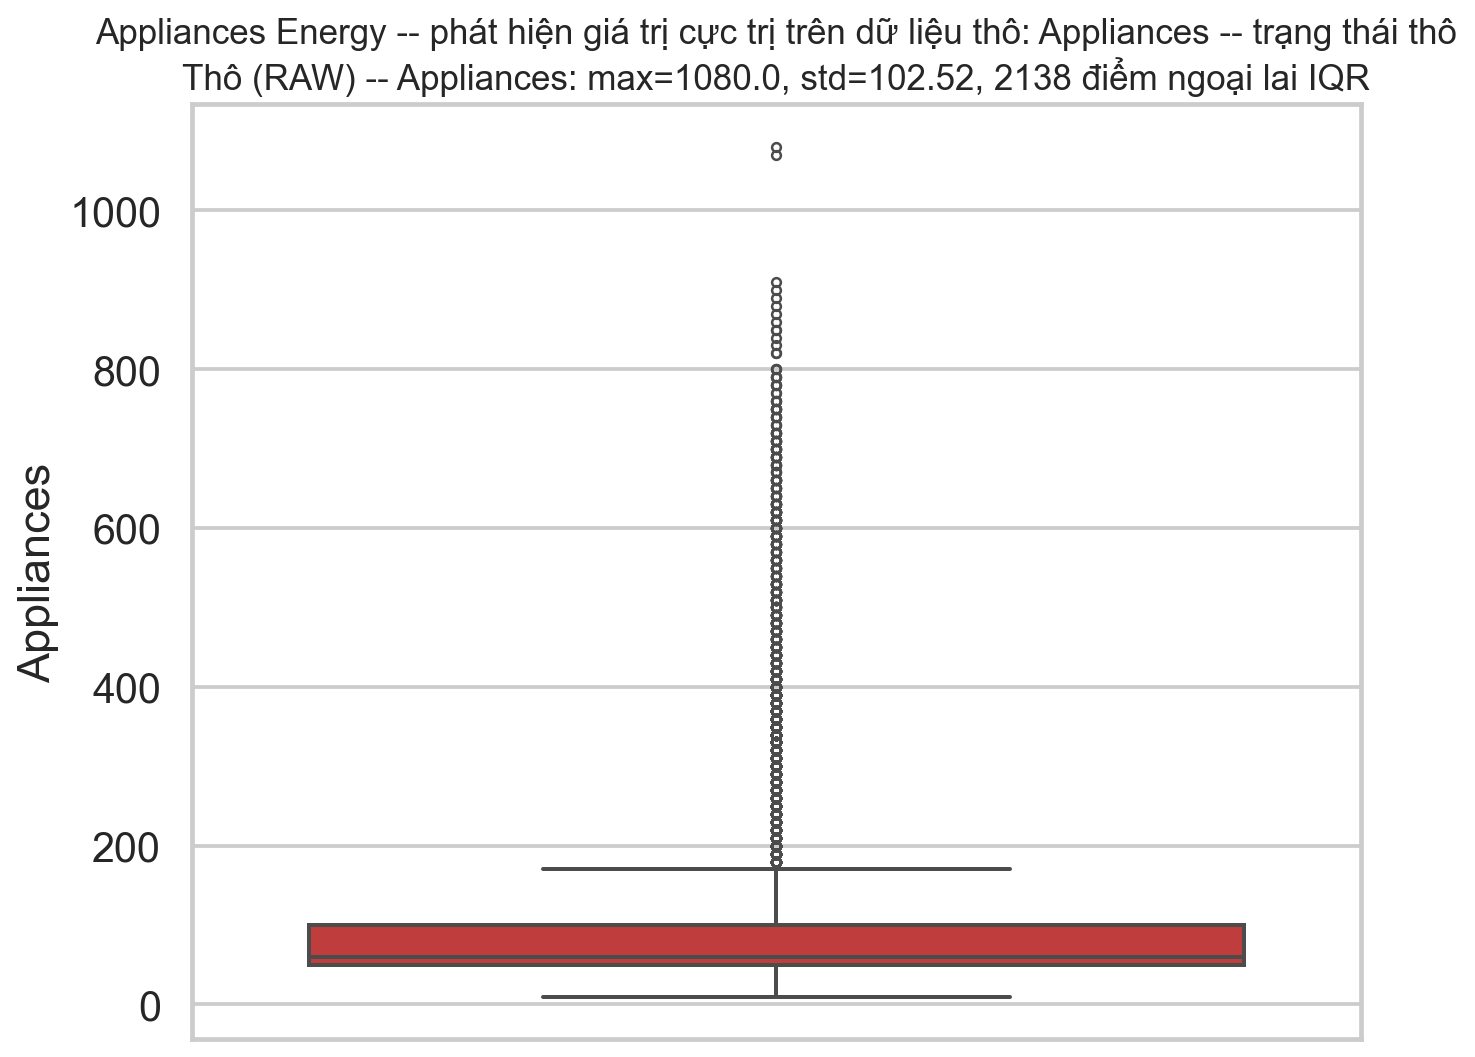
\includegraphics[width=0.72\textwidth]{images/ch3/appliances_energy_Appliances_boxplot_raw.png}
\captionsetup{justification=raggedright,singlelinecheck=false}
\caption[Boxplot \texttt{Appliances} thô]{Boxplot \texttt{Appliances} ở \textbf{trạng thái thô}: hàng nghìn điểm đỉnh tiêu thụ tới 1080 Wh (median 60). Đây là target dự báo nên sẽ \emph{không} clipping để bảo toàn giá trị thực.\\
\footnotesize Python source: \texttt{scripts/generate\_raw\_vs\_cleaned\_boxplots.py}.}
\label{fig:ch4_appliances_raw_boxplot}
\end{figure}

\textit{Phát hiện đoạn đứt/giá trị cực trị trên dữ liệu thô (line chart / boxplot).} Dưới boxplot trạng thái thô (Hình~\ref{fig:ch4_appliances_raw_boxplot}), vì chuỗi thực không có NaN nên line chart trạng thái thô (Hình~\ref{fig:ch4_appliances_daily_line}) \emph{không bị đứt gãy}; tuy nhiên, line chart và boxplot cho thấy: (a) biến mục tiêu \texttt{Appliances} có các \textbf{đỉnh tiêu thụ tới 1080 Wh} trong khi median chỉ 60 Wh, tạo các gai nhọn trên line chart và rất nhiều điểm ngoại lai trên boxplot -- đây là các đợt dùng điện đột biến, không phải lỗi; (b) Hình~\ref{fig:ch4_appliances_missing_fill} minh họa \emph{kịch bản đứt gãy}: nếu chuỗi cảm biến 10 phút bị mất tín hiệu (NaN) tại một khoảng ngắn, line chart sẽ bị ngắt thành hai đoạn rời; sau điền khuyết thì nối liền. Đây là cơ sở để áp dụng phương pháp điền khuyết chuỗi.

\textbf{Làm sạch dữ liệu.} Các bước làm sạch và biến đổi dữ liệu:

\begin{itemize}[leftmargin=*]
    \item \textbf{Sắp xếp theo thời gian:} đảm bảo thứ tự chuỗi đúng trước mọi xử lý.
    \item \textbf{Điền khuyết dự phòng:} linear interpolation + forward fill + backward fill, đề phòng chuỗi có khoảng trống do lỗi thu thập.
    \item \textbf{Xử lý ngoại lai:} \emph{clipping IQR} trên các biến đầu vào (\texttt{T1}, \texttt{RH\_1}, \texttt{T\_out}, \ldots) -- \emph{trừ} target \texttt{Appliances}, giữ nguyên để dự báo giá trị thực.
    \item \textbf{Log-transform:} \texttt{Appliances\_log1p = log(1+Appliances)} để nén đỉnh tiêu thụ lớn.
    \item \textbf{Differencing:} \texttt{Appliances\_diff} bậc một để chuyển sang tốc độ thay đổi.
\end{itemize}

\begin{figure}[H]
\centering
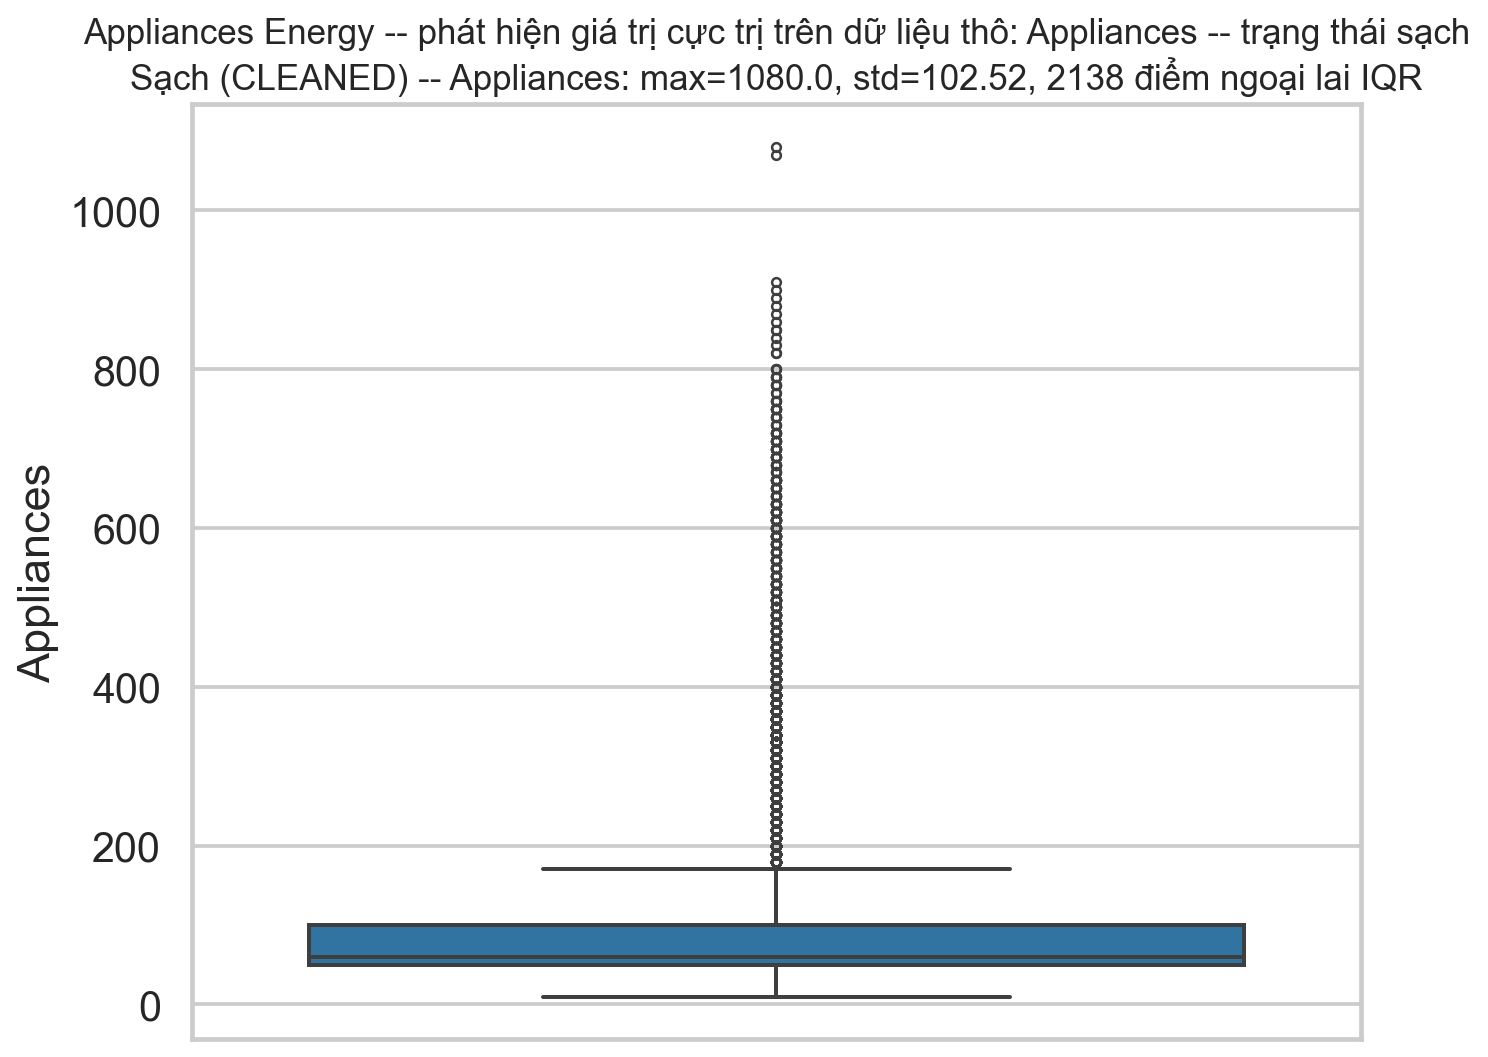
\includegraphics[width=0.72\textwidth]{images/ch3/appliances_energy_Appliances_boxplot_cleaned.png}
\captionsetup{justification=raggedright,singlelinecheck=false}
\caption[Boxplot \texttt{Appliances} sạch]{Boxplot \texttt{Appliances} ở \textbf{trạng thái sạch}: vì đây là target dự báo nên gần như giữ nguyên so với trạng thái thô (các đỉnh 1080 Wh được bảo toàn); chỉ các biến đầu vào \texttt{T\_out}, \texttt{RH\_1} mới bị clipping IQR.\\
\footnotesize Python source: \texttt{scripts/generate\_raw\_vs\_cleaned\_boxplots.py}.}
\label{fig:ch4_appliances_cleaned_boxplot}
\end{figure}

\textbf{Bước 1--2. Phân loại biến và thống kê mô tả.} Mọi biến đầu vào là Quantitative Continuous dạng chuỗi thời gian/cảm biến; \texttt{Appliances} là biến mục tiêu Continuous (regression).

\begin{table}[H]
\centering
\caption[Thống kê mô tả Appliances Energy]{Thống kê mô tả các chuỗi tiêu biểu Appliances Energy. Source: \texttt{outputs/tables/appliances\_energy\_summary.csv}.}
\label{tab:ch4_appliances_stats}
\small
\begin{tabular}{lrrrrr}
\toprule
Biến & Mean & Median & Std & Min & Max \\
\midrule
\texttt{Appliances} & 97.69 & 60.00 & 102.52 & 10.00 & 1080.00 \\
\texttt{lights} & 3.80 & 0.00 & 7.94 & 0.00 & 70.00 \\
\texttt{T1} & 21.69 & 21.60 & 1.61 & 16.79 & 26.26 \\
\texttt{RH\_1} & 40.26 & 39.66 & 3.98 & 27.02 & 63.36 \\
\texttt{T\_out} & 7.41 & 6.92 & 5.32 & -5.00 & 26.10 \\
\bottomrule
\end{tabular}
\end{table}

\begin{table}[H]
\centering
\caption[Thống kê thô/sạch Appliances Energy]{So sánh thống kê mô tả Appliances Energy ở hai trạng thái: \textbf{thô} và \textbf{sạch}. Lưu ý \texttt{Appliances} (target) \emph{không đổi} vì không clipping; các biến đầu vào thay đổi nhẹ do clipping IQR. Source: \texttt{outputs/tables/appliances\_energy\_summary.csv}.}
\label{tab:ch4_appliances_stats_raw_clean}
\footnotesize
\setlength{\tabcolsep}{4pt}
\begin{tabular}{lcrrrrr}
\toprule
Biến & Trạng thái & Mean & Median & Std & Min & \textbf{Max} \\
\midrule
\texttt{Appliances} & thô & 97.69 & 60.00 & 102.52 & 10.00 & 1080.00 \\
 (target, không clip) & sạch & 97.69 & 60.00 & 102.52 & 10.00 & 1080.00 \\
\midrule
\texttt{T1} & thô & 21.69 & 21.60 & 1.61 & 16.79 & \textbf{26.26} \\
 & sạch & 21.69 & 21.60 & 1.58 & 18.00 & \textbf{25.36} \\
\midrule
\texttt{RH\_1} & thô & 40.26 & 39.66 & 3.98 & 27.02 & \textbf{63.36} \\
 & sạch & 40.25 & 39.66 & 3.94 & 28.73 & \textbf{51.67} \\
\midrule
\texttt{T\_out} & thô & 7.41 & 6.92 & 5.32 & -5.00 & \textbf{26.10} \\
 & sạch & 7.37 & 6.92 & 5.20 & -5.00 & \textbf{20.50} \\
\bottomrule
\end{tabular}
\end{table}

\textit{Nhận xét thô/sạch.} Khác với Nhóm A, sự thay đổi ở Appliances Energy rất nhỏ vì các biến đầu vào (nhiệt độ, độ ẩm) ít có ngoại lai; clipping chỉ nén một vài giá trị cực trị ở biên (ví dụ \texttt{RH\_1} max 63.36$\to$51.67, \texttt{T\_out} max 26.10$\to$20.50). Quan trọng nhất, biến mục tiêu \texttt{Appliances} \emph{giữ nguyên hoàn toàn} ở cả hai trạng thái -- đây là quy tắc cốt lõi trong dự báo chuỗi thời gian: không clipping target để mô hình học đúng giá trị thực, kể cả các đỉnh tiêu thụ 1080 Wh.

\begin{table}[H]
\centering
\caption[Thông tin thời gian Appliances Energy]{Thông tin thời gian của chuỗi Appliances Energy. Source: \texttt{outputs/tables/appliances\_energy\_time\_info.csv}.}
\label{tab:ch4_appliances_time_info}
\small
\begin{tabular}{lr}
\toprule
Chỉ tiêu & Giá trị \\
\midrule
Bắt đầu & 2016-01-11 17:00:00 \\
Kết thúc & 2016-05-27 18:00:00 \\
Số quan sát & 19\,735 \\
Tần suất mode & 10 phút \\
\bottomrule
\end{tabular}
\end{table}

\textbf{Bước 3. Trực quan hóa (line chart, rolling, điền khuyết, raw vs log, differencing, ridgeline).}

\begin{figure}[H]\centering
\begin{subfigure}{0.90\textwidth}\centering\includegraphics[width=\textwidth]{images/ch3/appliances_energy_daily_line.png}\caption{Python -- Daily line chart}\end{subfigure}
\par\medskip
\begin{subfigure}{0.90\textwidth}\centering\includegraphics[width=\textwidth]{images/ch3/excel_appliances_daily_line_preview.png}\caption{Excel -- Daily line chart}\end{subfigure}
\caption[Line chart Appliances Energy: Python và Excel]{Xu hướng tiêu thụ điện trung bình theo ngày.\\
\footnotesize Python source: \texttt{src/analyze\_appliances\_energy.py}. Excel source/workbook: \texttt{src/create\_excel\_visualizations.py}, \texttt{excel/excel\_visualization\_comparison\_native.xlsx}, sheet \texttt{Appliances Daily}.}
\label{fig:ch4_appliances_daily_line}
\end{figure}
\textbf{Nhận xét Hình \ref{fig:ch4_appliances_daily_line}.} Line chart cho thấy mức tiêu thụ dao động mạnh theo ngày, không phù hợp chia train/test ngẫu nhiên. Cần giữ thứ tự thời gian để tránh rò rỉ thông tin tương lai.

\begin{figure}[H]\centering
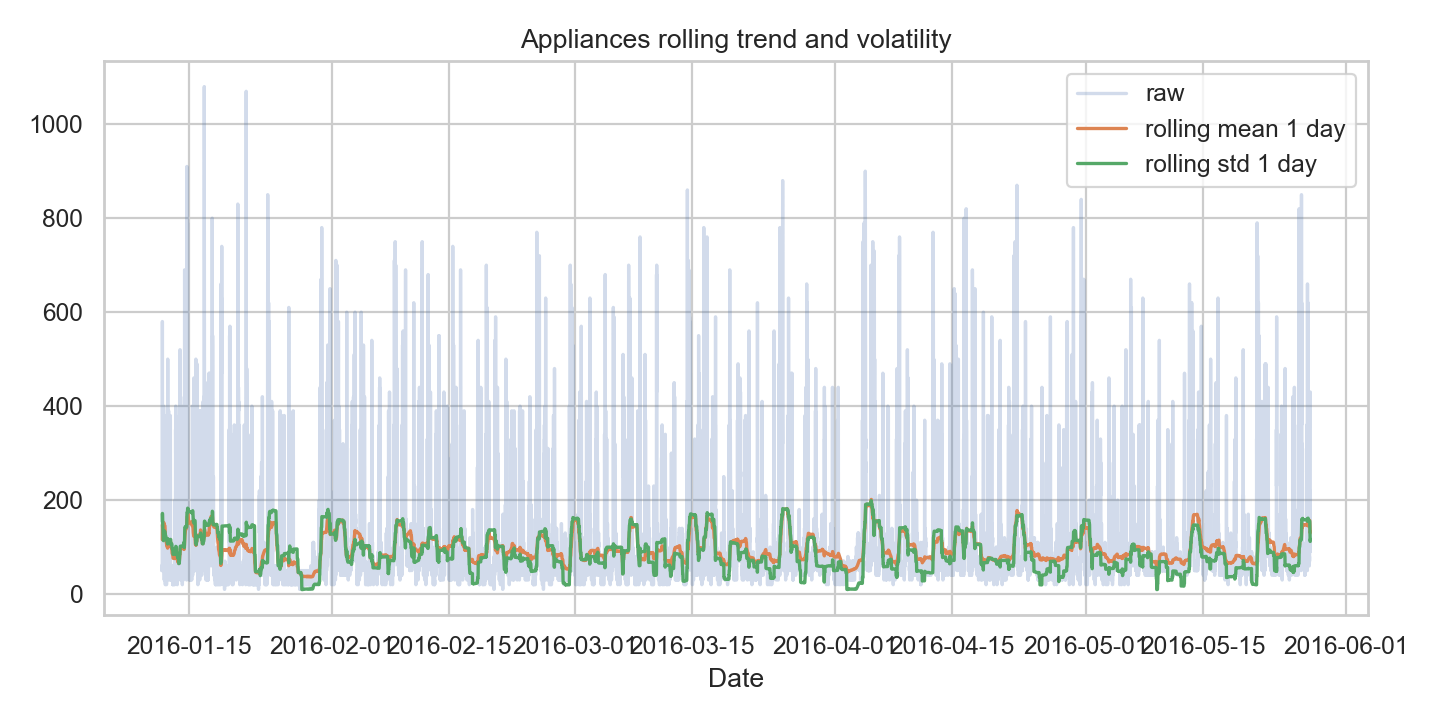
\includegraphics[width=0.90\textwidth]{images/ch3/appliances_energy_rolling_trend.png}
\caption[Rolling statistics Appliances Energy]{Rolling mean và rolling standard deviation 1 ngày của \texttt{Appliances}.\\
\footnotesize Python source: \texttt{scripts/generate\_group\_b\_figures.py}.}
\label{fig:ch4_appliances_rolling}
\end{figure}
\textbf{Nhận xét Hình \ref{fig:ch4_appliances_rolling}.} Rolling mean làm rõ xu hướng nền, còn rolling std cho thấy phương sai thay đổi theo thời gian. Đây là dấu hiệu chuỗi không hoàn toàn dừng.

\begin{figure}[H]\centering
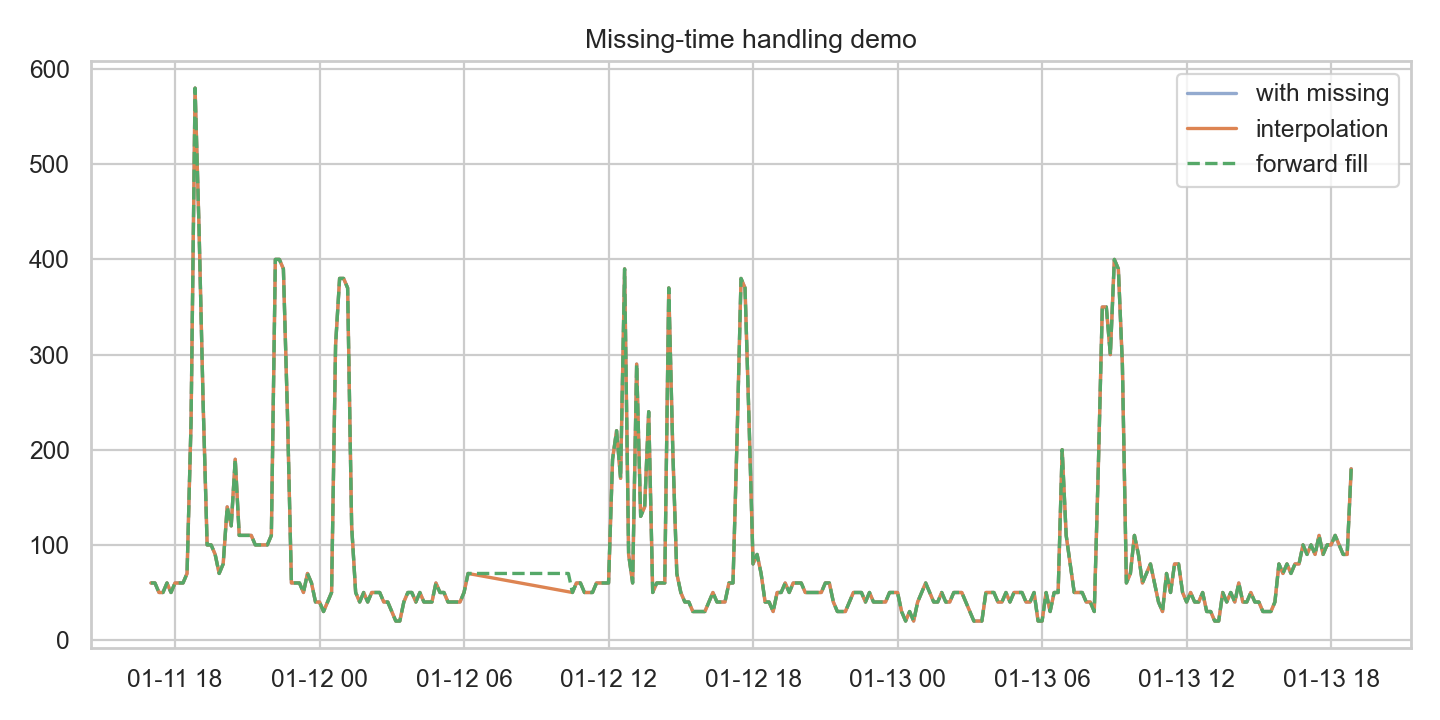
\includegraphics[width=0.90\textwidth]{images/ch3/appliances_energy_missing_interpolation_ffill.png}
\caption[Điền khuyết thời gian Appliances Energy]{Minh họa xử lý missing theo thời gian bằng interpolation và forward fill.\\
\footnotesize Python source: \texttt{scripts/generate\_group\_b\_figures.py}.}
\label{fig:ch4_appliances_missing_fill}
\end{figure}
\textbf{Nhận xét Hình \ref{fig:ch4_appliances_missing_fill}.} Interpolation tạo đường chuyển tiếp mượt giữa hai điểm quan sát, còn forward fill giữ giá trị gần nhất. Ở trạng thái thô, các khoảng Null/NaN tạo đoạn rỗng hoặc đứt gãy trên line chart; sau xử lý, chuỗi liền mạch hơn nên rolling mean, rolling std và mô hình dự báo không bị ngắt do thiếu điểm. Với chuỗi cảm biến 10 phút, interpolation phù hợp khi missing ngắn; forward fill phù hợp khi trạng thái vật lý ít thay đổi.

\begin{figure}[H]\centering
\begin{subfigure}{0.90\textwidth}\centering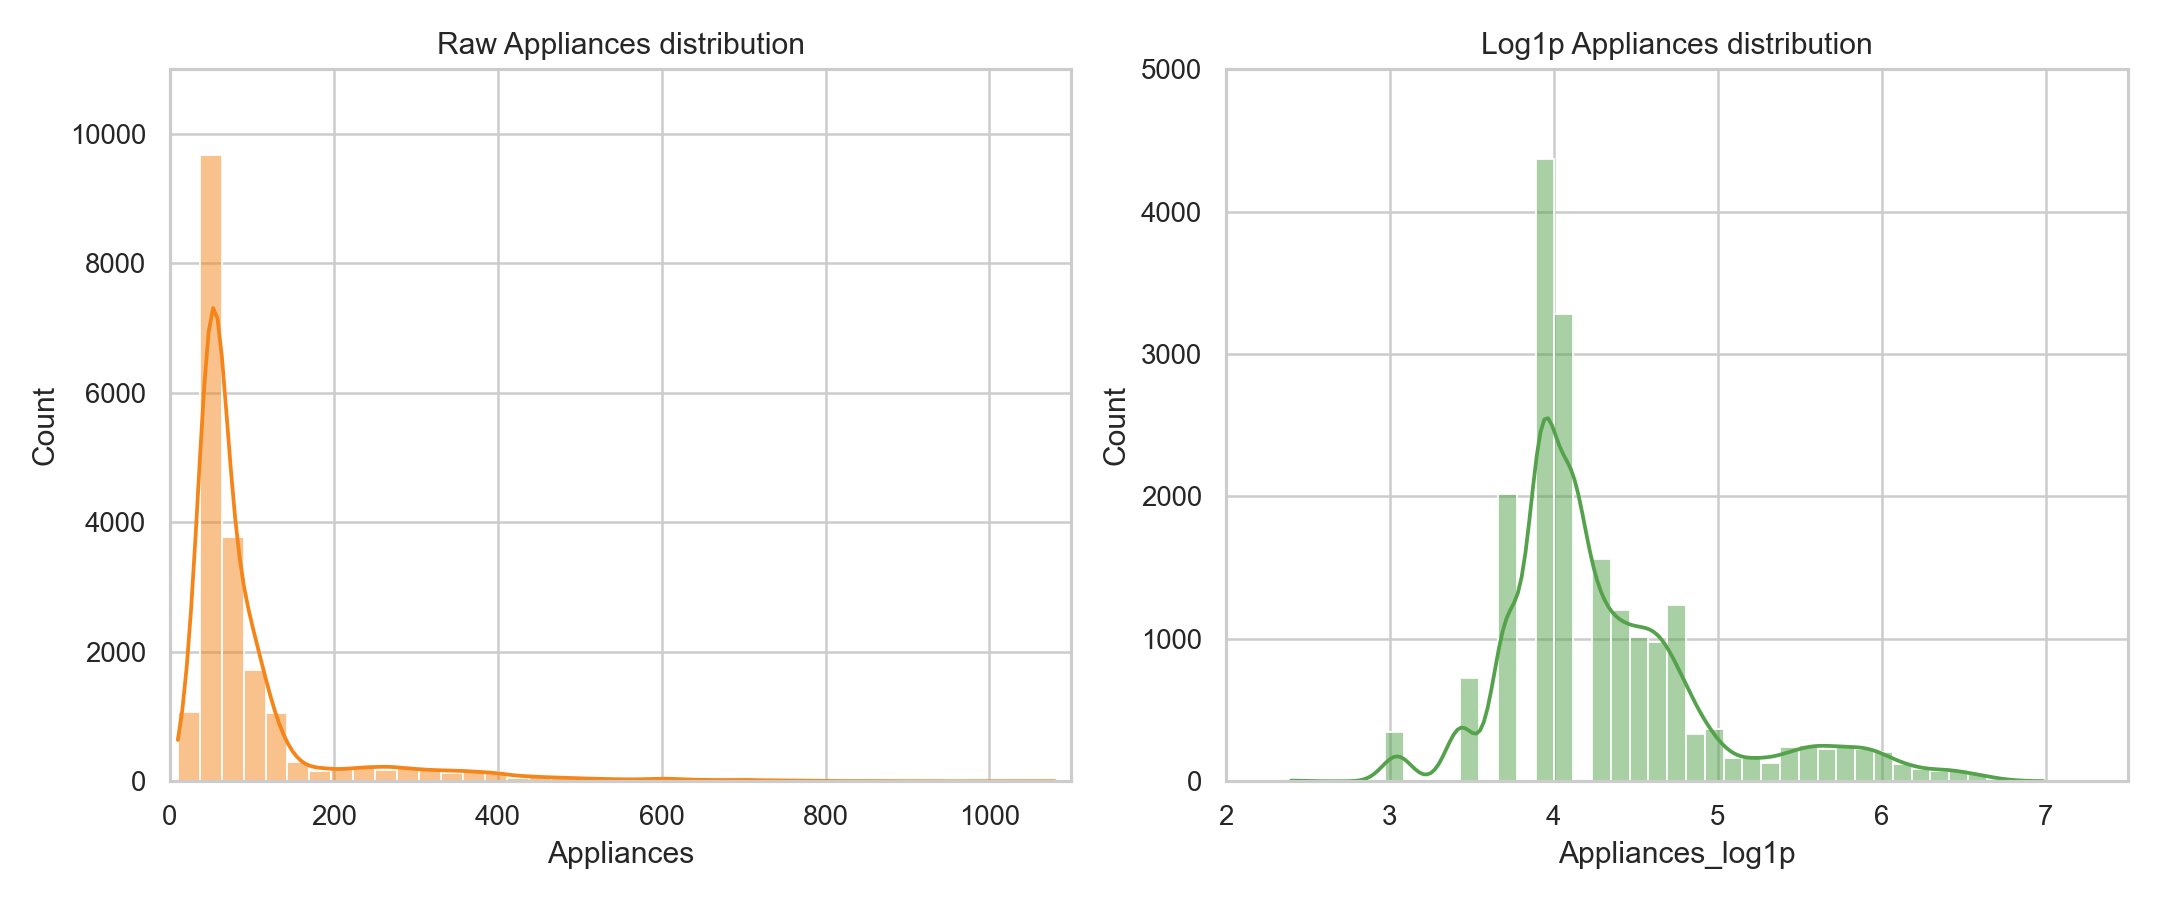
\includegraphics[width=\textwidth]{images/ch3/appliances_energy_distribution_raw_vs_log.png}\caption{Python -- Raw vs log1p}\end{subfigure}
\par\medskip
\begin{subfigure}{0.90\textwidth}\centering\includegraphics[width=\textwidth]{images/ch3/excel_appliances_raw_vs_log_hist_preview.png}\caption{Excel -- Raw vs log1p}\end{subfigure}
\caption[Log-transform Appliances Energy: Python và Excel]{Biến đổi \texttt{log1p} để giảm lệch phải của \texttt{Appliances}.\\
\footnotesize Python source: \texttt{src/analyze\_appliances\_energy.py}. Excel source/workbook: \texttt{src/create\_excel\_visualizations.py}, \texttt{excel/excel\_visualization\_comparison\_native.xlsx}, sheet \texttt{Appliances Histogram}.}
\label{fig:ch4_appliances_log}
\end{figure}
\textbf{Nhận xét Hình \ref{fig:ch4_appliances_log}.} Phân phối gốc lệch phải mạnh do các đỉnh tiêu thụ cao. \texttt{log1p} nén đuôi phải, giúp phương sai ổn định hơn.

\begin{figure}[H]\centering
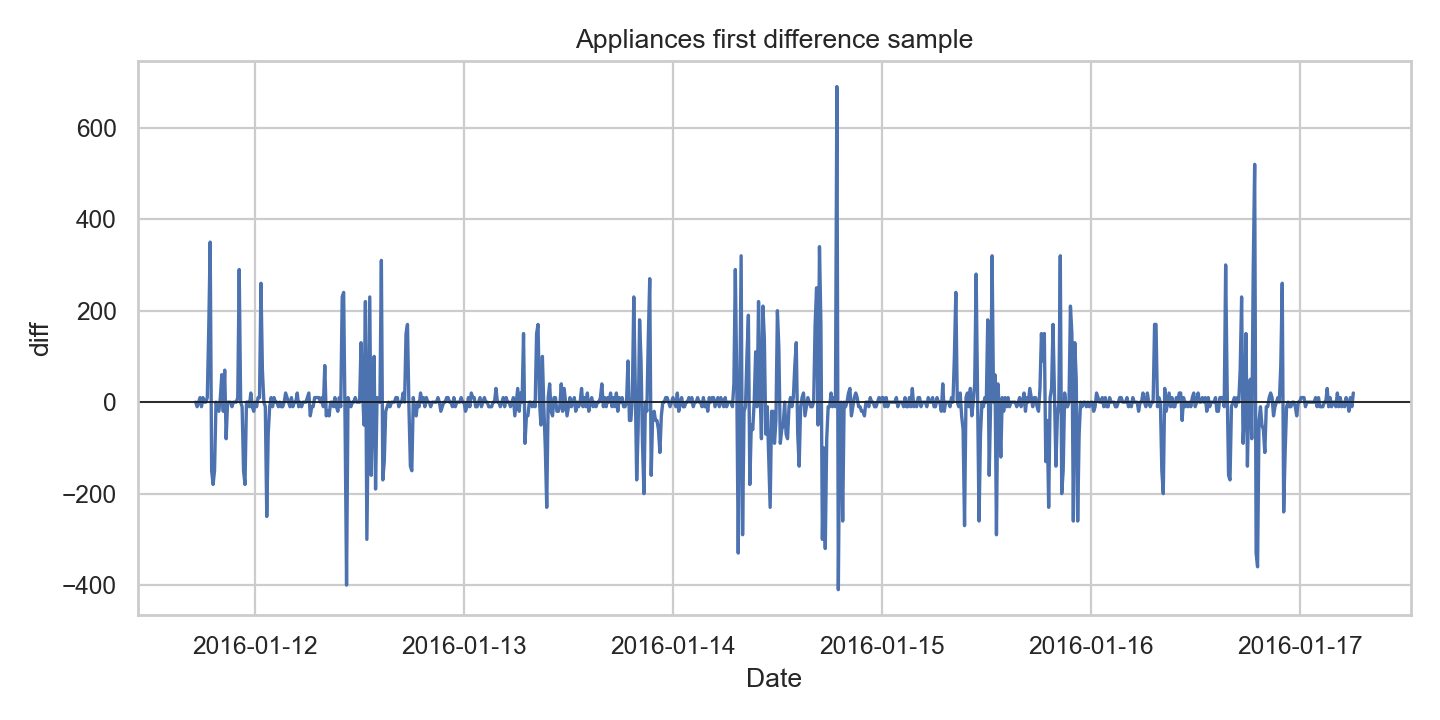
\includegraphics[width=0.90\textwidth]{images/ch3/appliances_energy_differencing_line.png}
\caption[Differencing Appliances Energy]{Sai phân bậc một của \texttt{Appliances}.\\
\footnotesize Python source: \texttt{scripts/generate\_group\_b\_figures.py}.}
\label{fig:ch4_appliances_diff}
\end{figure}
\textbf{Nhận xét Hình \ref{fig:ch4_appliances_diff}.} Differencing đưa chuỗi về dao động quanh 0, giúp nhấn mạnh thay đổi ngắn hạn thay vì mức tuyệt đối.

\begin{figure}[H]\centering
\begin{subfigure}{0.90\textwidth}\centering\includegraphics[width=\textwidth]{images/ch3/appliances_energy_monthly_ridgeline.png}\caption{Python -- Monthly ridgeline}\end{subfigure}
\caption[Mùa vụ Appliances Energy]{Phân phối \texttt{log1p(Appliances)} theo tháng.\
\footnotesize Python source: \texttt{src/analyze\_appliances\_energy.py}.\
}\label{fig:ch4_appliances_seasonality}
\end{figure}
\textbf{Nhận xét Hình \ref{fig:ch4_appliances_seasonality}.} Ridgeline cho thấy hình dạng phân phối thay đổi theo tháng, gợi ý ảnh hưởng mùa vụ và điều kiện thời tiết ngoài trời.

\textbf{Bước 4. So sánh trước--sau biến đổi chuỗi.} Trạng thái thô và trạng thái sạch của Appliances Energy khác ở ba phép biến đổi chính, mỗi phép được minh chứng bằng một biểu đồ: (1) \emph{điền khuyết} -- Hình~\ref{fig:ch4_appliances_missing_fill} cho thấy line chart của chuỗi thô có thể đứt gãy tại các NaN, còn sau interpolation/forward fill thì liền mạch; (2) \emph{log-transform} -- Hình~\ref{fig:ch4_appliances_log} đặt histogram \texttt{Appliances} thô (lệch phải mạnh, đuôi tới 1080) cạnh histogram \texttt{log1p(Appliances)} (gần đối xứng hơn); (3) \emph{differencing} -- Hình~\ref{fig:ch4_appliances_diff} cho thấy chuỗi sai phân dao động quanh 0. \textbf{Nhận xét so sánh:} chuỗi thô có std rất lớn (102.52) và phân phối đỉnh lệch, chuỗi sau log-transform có std nhỏ hơn rõ và gần chuẩn hơn -- đây là điều kiện quan trọng cho các mô hình tuyến tính và ARIMA. Differencing làm mất một bậc tự do nhưng loại bỏ trend, giúp chuỗi dừng hơn. Vì dữ liệu gốc không có missing thực, ``trạng thái sạch'' ở đây chủ yếu là \emph{biến đổi chuỗi} chứ không phải điền khuyết; báo cáo trình bày trung thực điều này.

\subsubsection{Human Activity Recognition Using Smartphones}

HAR có 10\,299 quan sát và 561 đặc trưng cảm biến đã trích xuất. Năm chuỗi/feature chọn để phân tích gồm \texttt{f001\_tBodyAcc-mean()-X}, \texttt{f002\_tBodyAcc-mean()-Y}, \texttt{f003\_tBodyAcc-mean()-Z}, \texttt{f004\_tBodyAcc-std()-X}, \texttt{f005\_tBodyAcc-std()-Y}.

\textbf{Trạng thái dữ liệu thô (chưa làm sạch).} HAR của UCI đã được \emph{tiền xử lý sẵn} ở nguồn: tín hiệu gia tốc/gyro được lọc nhiễu, chia cửa sổ trượt 2.56~s, trích xuất 561 đặc trưng và chuẩn hóa trong khoảng $[-1,1]$. Do đó bộ dữ liệu \emph{không có ô khuyết thiếu} và không yêu cầu điền khuyết/clipping ở giai đoạn này; ``trạng thái thô'' và ``trạng thái sạch'' gần như trùng nhau. Dù vậy, vì đây là dữ liệu chuỗi cảm biến, quy trình Nhóm B vẫn kiểm tra hai điều kiện thời gian: (1) \emph{đứt gãy trên line chart} -- Hình~\ref{fig:ch4_har_line} cho thấy chuỗi liền mạch, không có khoảng NaN cần điền bằng forward/backward fill hay linear interpolation; (2) \emph{biến đổi chuỗi} -- vì các feature đã được chuẩn hóa $[-1,1]$ và trích xuất theo cửa sổ, log-transform và differencing không mang thêm giá trị ở cấp độ feature; thay vào đó, rolling statistics có thể dùng để quan sát xu hướng theo đoạn hoạt động.

\textit{Phát hiện trên dữ liệu thô (boxplot).} Trên boxplot 5 feature theo hoạt động (Hình~\ref{fig:ch4_har_box}), vẫn xuất hiện các điểm rời rạc ngoài râu IQR ở các feature gia tốc. Tuy nhiên, các điểm này thường là \emph{chuyển động thực sự mãnh liệt} (ví dụ chạy WALKING, nhảy) chứ không phải lỗi đo, đặc biệt feature \texttt{f001...X} ở nhóm hoạt động động có phân bố rộng và nhiều ngoại biên hơn nhóm tĩnh (SITTING/STANDING/LAYING). Vì vậy chúng \emph{không nên loại bỏ cơ học}; clipping sẽ làm mất chính tín hiệu cần phân loại.

\textit{Đứt gãy trên line chart.} Hình~\ref{fig:ch4_har_line} cho thấy line chart của 5 feature liền mạch (không có đoạn đứt), xác nhận dữ liệu đã hoàn chỉnh.

\textbf{Bước 1--2. Phân loại biến và thống kê.} Các feature là Quantitative Continuous đã chuẩn hóa $[-1,1]$; biến mục tiêu \texttt{Activity} là Qualitative nominal (6 lớp: WALKING, WALKING\_UPSTAIRS, WALKING\_DOWNSTAIRS, SITTING, STANDING, LAYING).

\textbf{Bước 3. Trực quan hóa (phân bố hoạt động, line chart, boxplot theo hoạt động, heatmap tương quan).}

\begin{figure}[H]\centering
\begin{subfigure}{0.90\textwidth}\centering\includegraphics[width=\textwidth]{images/ch3/har_activity_distribution.png}\caption{Python -- Activity distribution}\end{subfigure}
\caption[Phân bố hoạt động HAR]{Tần suất các hoạt động trong HAR.\
\footnotesize Python source: \texttt{src/analyze\_har.py}.\
}\label{fig:ch4_har_activity}
\end{figure}
\textbf{Nhận xét Hình \ref{fig:ch4_har_activity}.} Các lớp hoạt động tương đối cân bằng, thuận lợi cho phân loại nhiều lớp; vẫn cần kiểm tra từng lớp động/tĩnh vì tín hiệu cảm biến có độ biến thiên khác nhau.

\begin{figure}[H]\centering
\begin{subfigure}{0.90\textwidth}\centering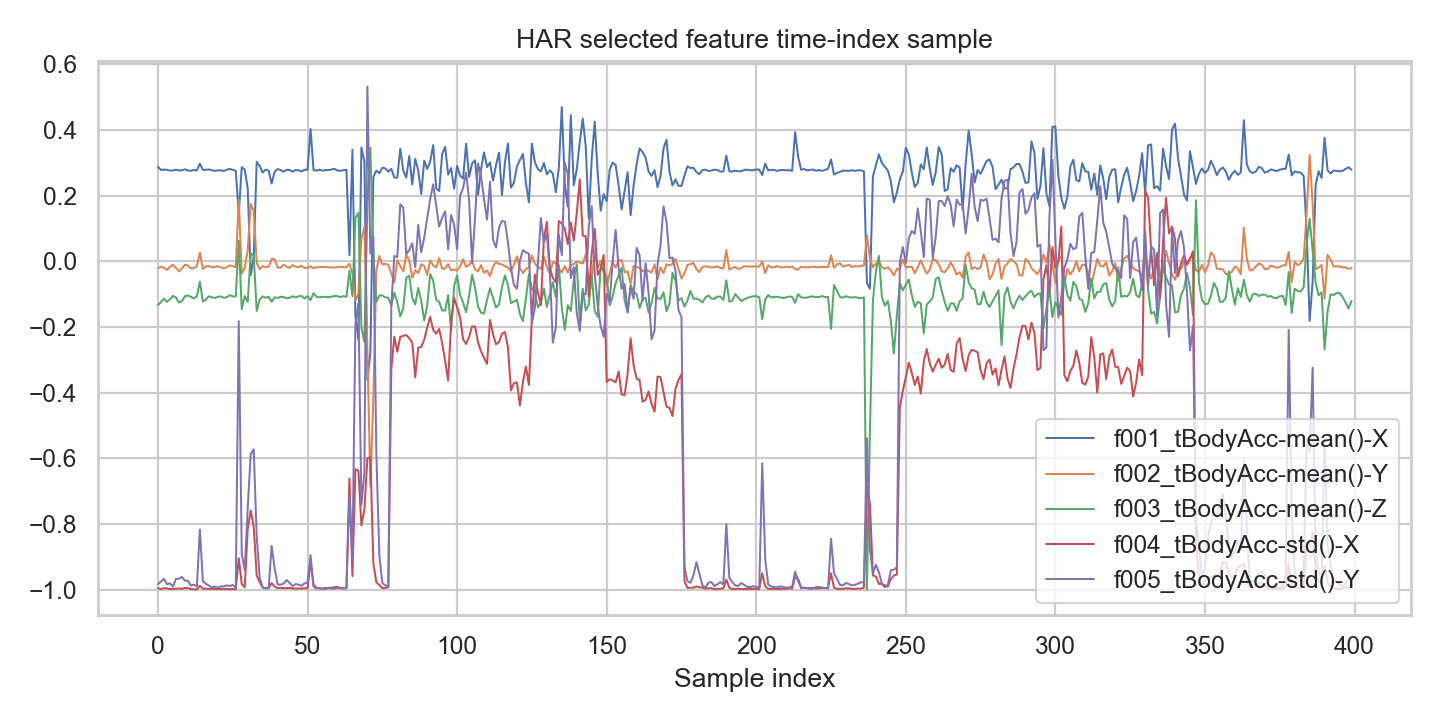
\includegraphics[width=\textwidth]{images/ch3/har_selected_feature_line.png}\caption{Python -- Feature line sample}\end{subfigure}
\caption[Line chart HAR]{Line chart theo index mẫu của 5 feature HAR đã chọn.\
\footnotesize Python source: \texttt{scripts/generate\_group\_b\_figures.py}.\
}\label{fig:ch4_har_line}
\end{figure}
\textbf{Nhận xét Hình \ref{fig:ch4_har_line}.} Line chart cho thấy các feature tăng/giảm theo đoạn hoạt động; vì vậy khi chia dữ liệu cần chú ý subject và activity block, không chỉ coi mẫu là độc lập tuyệt đối.

\begin{figure}[H]\centering
\begin{subfigure}{0.90\textwidth}\centering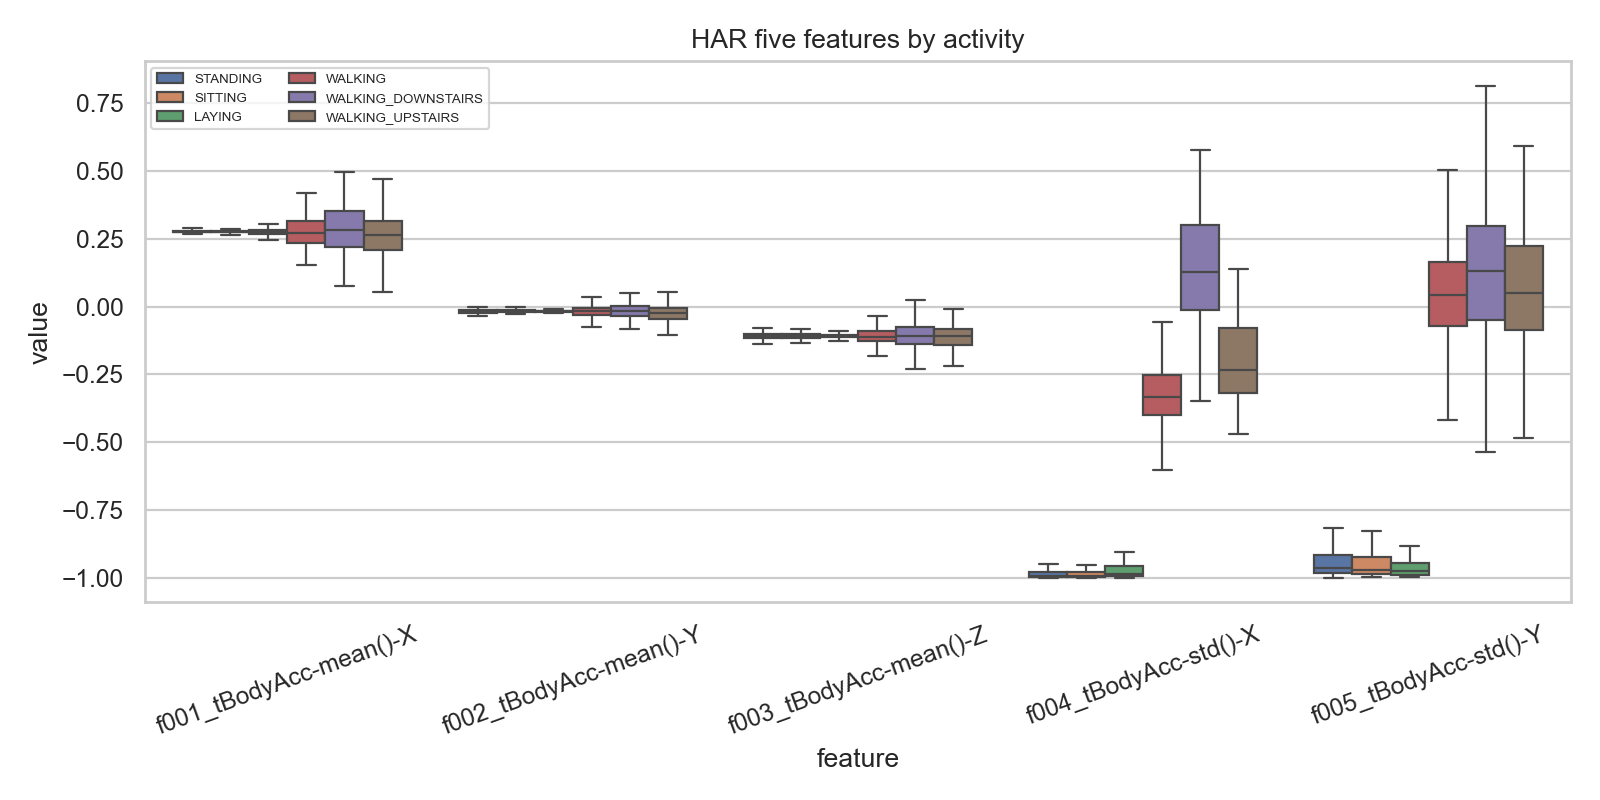
\includegraphics[width=\textwidth]{images/ch3/har_five_feature_boxplot.png}\caption{Python -- Boxplot 5 features}\end{subfigure}
\caption[Boxplot HAR]{Boxplot 5 feature HAR theo hoạt động.\
\footnotesize Python source: \texttt{scripts/generate\_group\_b\_figures.py}.\
}\label{fig:ch4_har_box}
\end{figure}
\textbf{Nhận xét Hình \ref{fig:ch4_har_box}.} Feature mean/std tách rõ giữa nhóm hoạt động tĩnh và động. Các giá trị ngoại biên có thể là chuyển động thực, không nên loại bỏ cơ học.

\begin{figure}[H]\centering
\begin{subfigure}{0.90\textwidth}\centering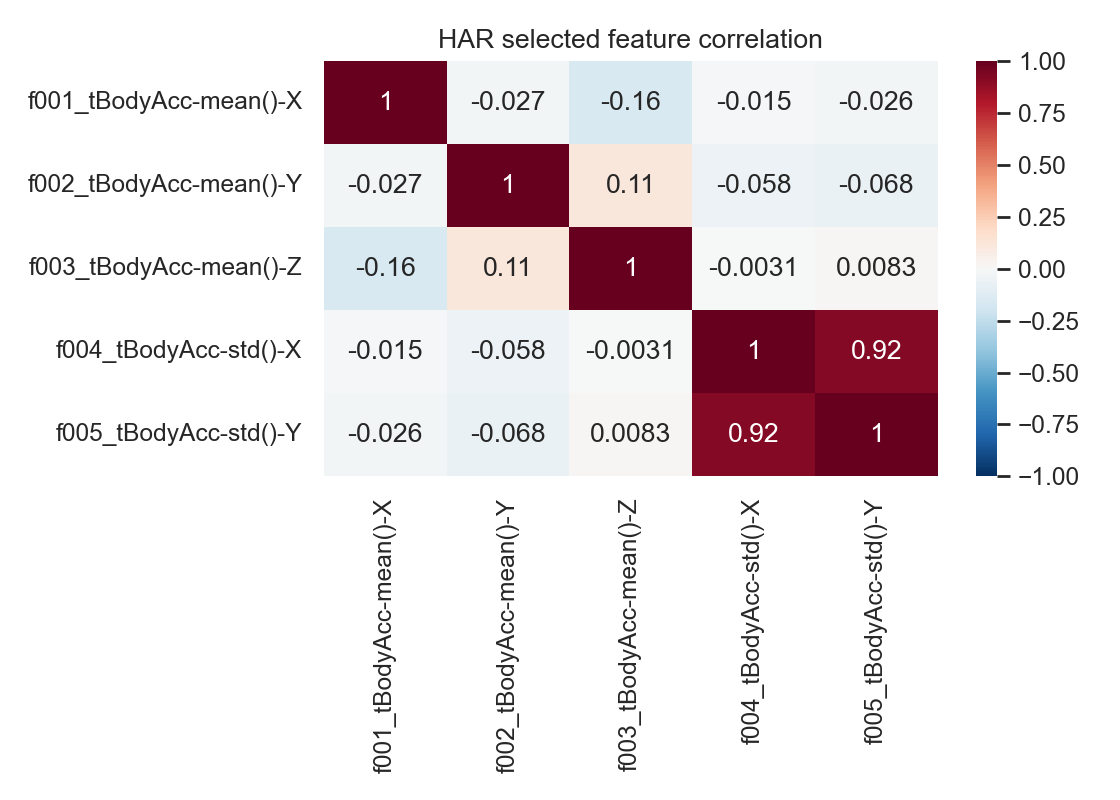
\includegraphics[width=\textwidth]{images/ch3/har_selected_feature_correlation_heatmap.png}\caption{Python -- Correlation heatmap}\end{subfigure}
\caption[Heatmap HAR]{Heatmap tương quan 5 feature HAR.\
\footnotesize Python source: \texttt{scripts/generate\_group\_b\_figures.py}.\
}\label{fig:ch4_har_corr}
\end{figure}
\textbf{Nhận xét Hình \ref{fig:ch4_har_corr}.} Các trục gia tốc có tương quan nhất định, nhưng không hoàn toàn trùng nhau; giữ nhiều trục giúp mô hình nhận diện hướng chuyển động.

\textbf{Bước 4. So sánh trước--sau.} Vì HAR đã chuẩn hóa sẵn và không có khuyết thiếu, ``trạng thái sạch'' không khác biệt đáng kể so với ``trạng thái thô'' -- điều này \emph{chính là một kết luận có giá trị}: dữ liệu cảm biến chất lượng cao, sẵn sàng cho mô hình mà không cần thêm làm sạch. Bài học rút ra cho mô hình là giữ lại các điểm ngoại biên mang ý nghĩa chuyển động, và chia train/test theo subject để tránh rò rỉ thông tin.

\subsubsection{MHEALTH}

MHEALTH là dữ liệu cảm biến đeo trên cơ thể. Sáu chuỗi chọn phân tích gồm \texttt{sensor\_01}, \texttt{sensor\_02}, \texttt{sensor\_03}, \texttt{sensor\_10}, \texttt{sensor\_11}, \texttt{sensor\_12}; các chuỗi này đại diện cho nhiều kênh cảm biến và hoạt động.

\textbf{Trạng thái dữ liệu thô (chưa làm sạch).} MHEALTH là tín hiệu cảm biến thô đã ghi liên tục ở 50~Hz; bộ dữ liệu \emph{không có ô khuyết thiếu} đáng kể. Trên line chart 6 sensor (Hình~\ref{fig:ch4_mhealth_line}), chuỗi \emph{liền mạch, không có đoạn đứt gãy}, xác nhận dữ liệu thu thập hoàn chỉnh -- do đó không cần áp dụng forward/backward fill hay linear interpolation.

\textit{Phát hiện trên dữ liệu thô (boxplot / line chart).} Trên boxplot sensor theo hoạt động (Hình~\ref{fig:ch4_mhealth_box}), xuất hiện nhiều điểm rời rạc ngoài râu IQR, đặc biệt ở các sensor gia tốc (\texttt{sensor\_01..03}). Các đỉnh đột biến này thường là \emph{chuyển động đột ngột hợp lệ} (ví dụ đá chân, gập người, nhảy), nên không nên clipping cơ học -- làm vậy sẽ mất chính các sự kiện hoạt động cần nhận dạng; dao động ngắn hạn mạnh trên line chart phản ánh chuyển động cơ thể thực.

\textbf{Làm sạch dữ liệu.} Vì dữ liệu cảm biến không có khuyết thiếu và các ngoại lai mang ý nghĩa chuyển động, các bước ``làm sạch'' tập trung vào \emph{biến đổi chuỗi thời gian} thay vì điền khuyết:

\begin{itemize}[leftmargin=*]
    \item \textbf{Điền khuyết chuỗi:} \emph{không cần áp dụng} -- dữ liệu thô đã liền mạch, không có đoạn NaN cần forward/backward fill hay linear interpolation.
    \item \textbf{Rolling statistics:} trung bình trượt (rolling mean) làm rõ mức nền của cảm biến, tách chuyển động chậm ra khỏi dao động nhanh.
    \item \textbf{Differencing:} hiệu phân bậc một của \texttt{sensor\_01} nhấn mạnh các \emph{thay đổi tức thời} -- đỉnh của chuỗi sai phân ứng với khoảnh khắc chuyển động đột ngột (ví dụ bắt đầu hoạt động), chính là tín hiệu quan trọng để nhận dạng hoạt động.
    \item \textbf{Kiểm tra nhãn:} lớp \texttt{NULL} (đoạn không gán nhãn hoạt động) chiếm tỷ lệ lớn và cần xử lý khi mô hình hóa.
\end{itemize}

Hai phép biến đổi rolling và differencing được minh họa trong Hình~\ref{fig:ch4_mhealth_roll_diff}.

\textbf{Bước 1--2. Phân loại biến và thống kê.} Các sensor là Quantitative Continuous (gia tốc, gyro); biến mục tiêu \texttt{Activity} là Qualitative nominal, trong đó lớp \texttt{NULL} chiếm tỷ lệ lớn.

\textbf{Bước 3. Trực quan hóa (phân bố hoạt động, line chart sensor, boxplot theo hoạt động, rolling/differencing, heatmap tương quan).}

\begin{figure}[H]\centering
\begin{subfigure}{0.90\textwidth}\centering\includegraphics[width=\textwidth]{images/ch3/mhealth_activity_distribution.png}\caption{Python -- Activity distribution}\end{subfigure}
\caption[Phân bố hoạt động MHEALTH]{Tần suất hoạt động trong mẫu MHEALTH.\
\footnotesize Python source: \texttt{src/analyze\_mhealth.py}.\
}\label{fig:ch4_mhealth_activity}
\end{figure}
\textbf{Nhận xét Hình \ref{fig:ch4_mhealth_activity}.} Lớp NULL chiếm tỷ lệ lớn do nhiều đoạn không gán hoạt động; phân tích mô hình nên cân nhắc lọc NULL hoặc dùng class weight.

\begin{figure}[H]\centering
\begin{subfigure}{0.90\textwidth}\centering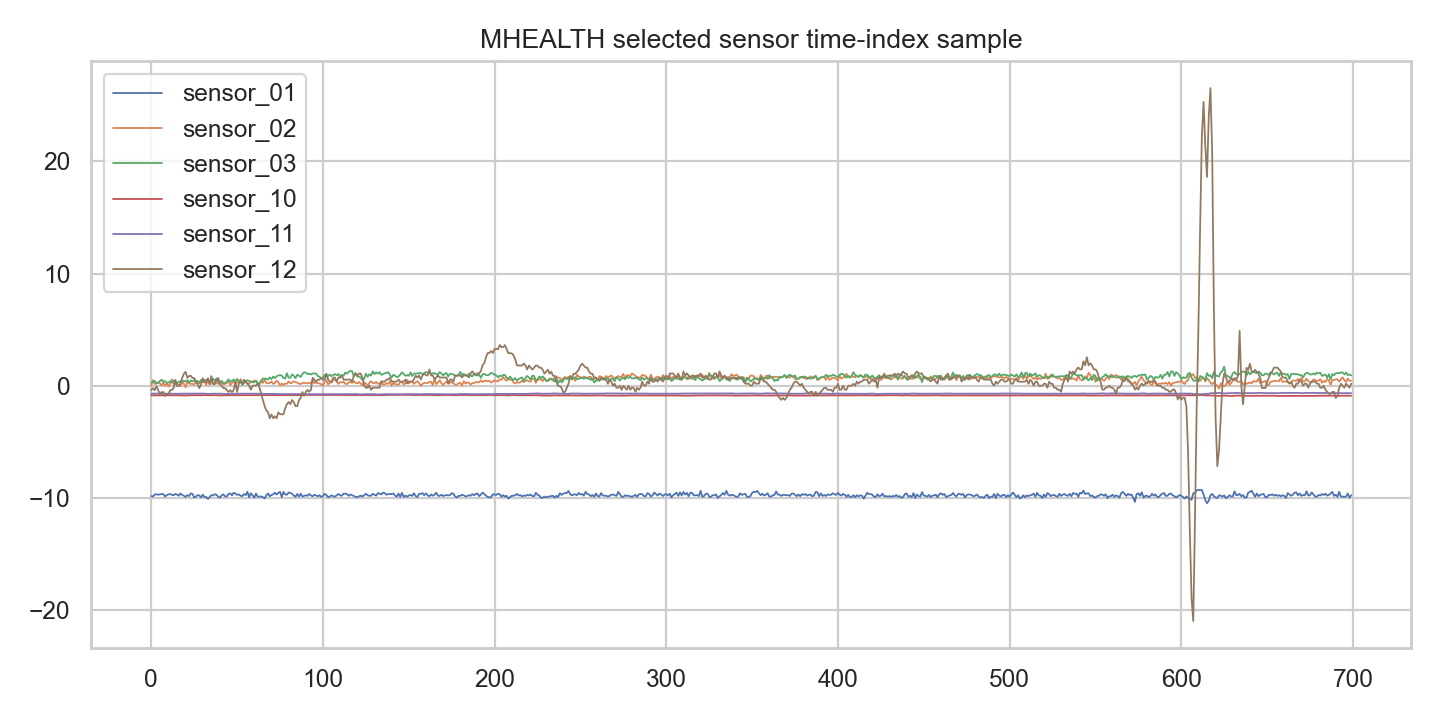
\includegraphics[width=\textwidth]{images/ch3/mhealth_selected_sensor_line.png}\caption{Python -- Sensor line sample}\end{subfigure}
\caption[Line chart MHEALTH]{Line chart theo index mẫu của 6 sensor MHEALTH.\
\footnotesize Python source: \texttt{scripts/generate\_group\_b\_figures.py}.\
}\label{fig:ch4_mhealth_line}
\end{figure}
\textbf{Nhận xét Hình \ref{fig:ch4_mhealth_line}.} Chuỗi sensor có dao động ngắn hạn mạnh, phản ánh chuyển động cơ thể. Biểu đồ đường phù hợp hơn histogram khi cần đọc đoạn hoạt động liên tiếp.

\begin{figure}[H]\centering
\begin{subfigure}{0.90\textwidth}\centering\includegraphics[width=\textwidth]{images/ch3/mhealth_sensor_boxplot.png}\caption{Python -- Sensor boxplot}\end{subfigure}
\caption[Boxplot MHEALTH]{Boxplot sensor theo hoạt động MHEALTH.\
\footnotesize Python source: \texttt{src/analyze\_mhealth.py}.\
}\label{fig:ch4_mhealth_box}
\end{figure}
\textbf{Nhận xét Hình \ref{fig:ch4_mhealth_box}.} Phân bố sensor khác nhau giữa các hoạt động; ngoại lai có thể là chuyển động đột ngột nên cần kiểm tra theo ngữ cảnh trước khi clipping.

\begin{figure}[H]\centering
\begin{subfigure}{0.90\textwidth}\centering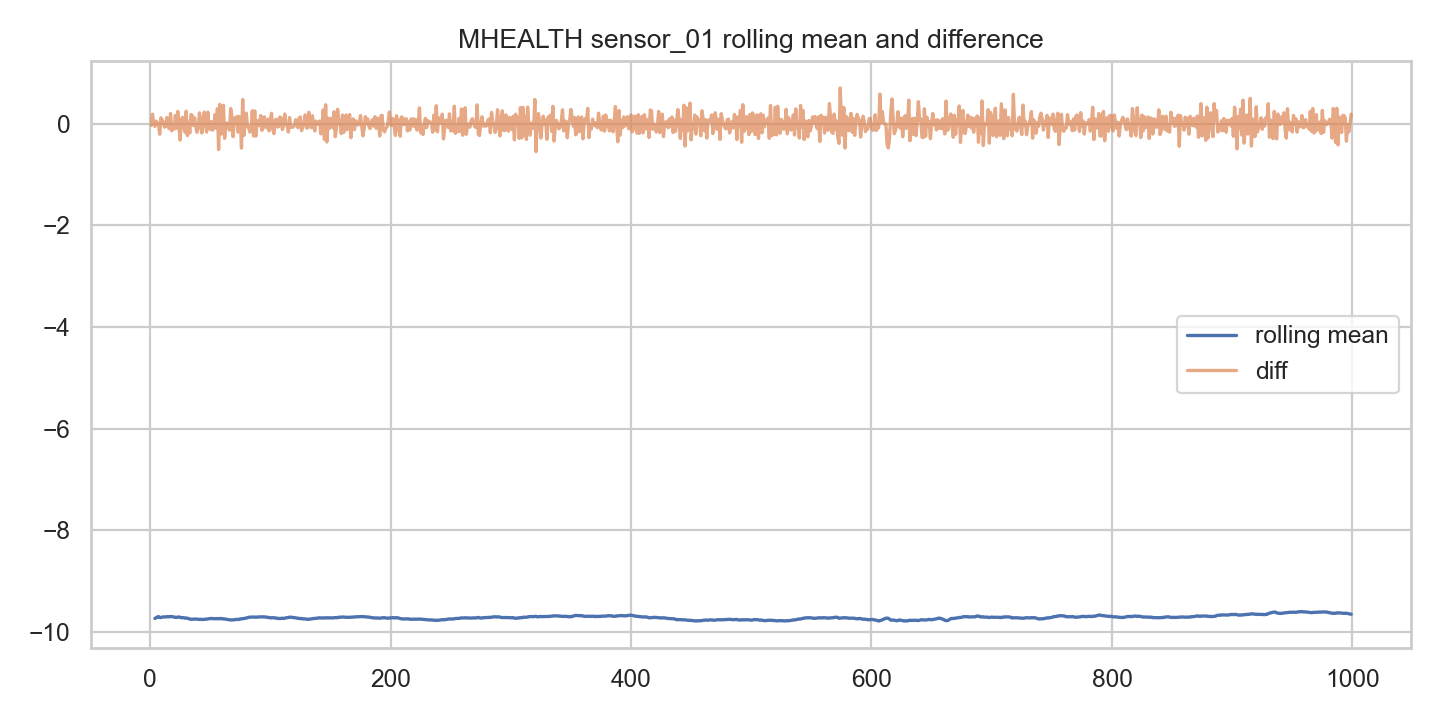
\includegraphics[width=\textwidth]{images/ch3/mhealth_sensor_rolling_diff.png}\caption{Python -- Rolling/differencing}\end{subfigure}
\caption[Rolling và differencing MHEALTH]{Rolling mean và sai phân của \texttt{sensor\_01}.\
\footnotesize Python source: \texttt{scripts/generate\_group\_b\_figures.py}.\
}\label{fig:ch4_mhealth_roll_diff}
\end{figure}
\textbf{Nhận xét Hình \ref{fig:ch4_mhealth_roll_diff}.} Rolling mean làm rõ mức nền của cảm biến, còn differencing nhấn mạnh thay đổi tức thời; hai cách nhìn này bổ sung cho phân tích hoạt động.

\begin{figure}[H]\centering
\begin{subfigure}{0.90\textwidth}\centering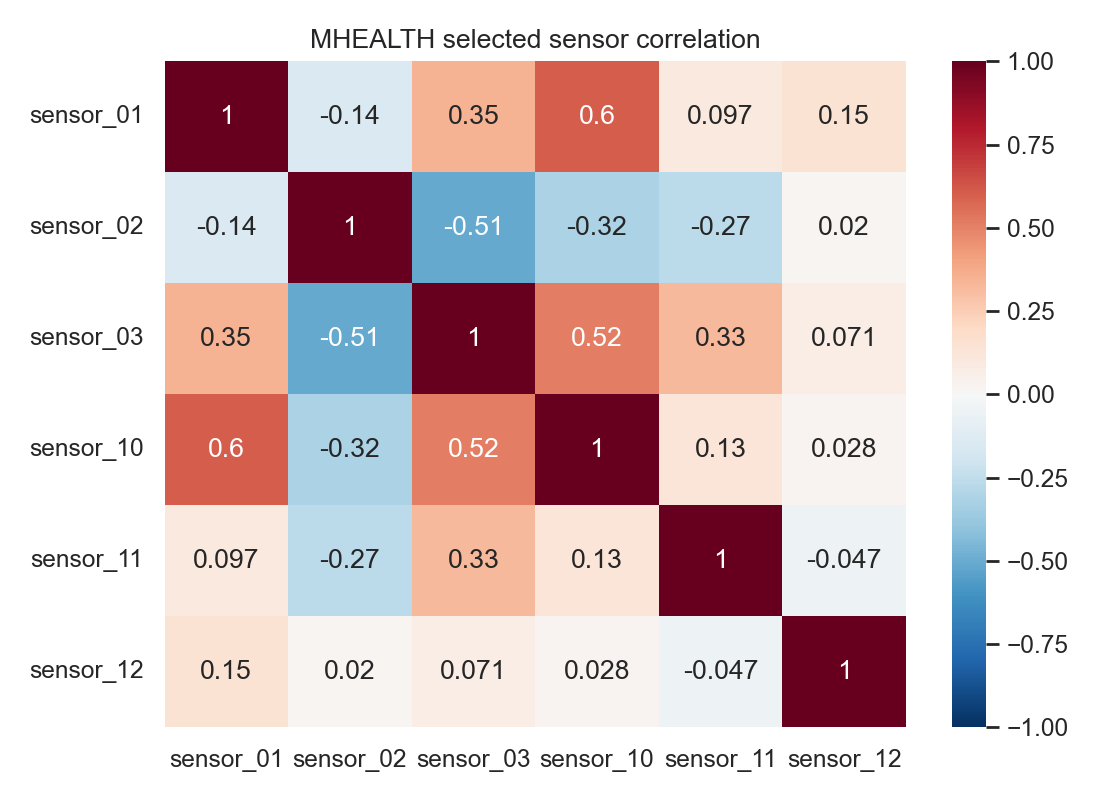
\includegraphics[width=\textwidth]{images/ch3/mhealth_sensor_correlation_heatmap.png}\caption{Python -- Correlation heatmap}\end{subfigure}
\caption[Heatmap MHEALTH]{Heatmap tương quan các sensor MHEALTH đã chọn.\
\footnotesize Python source: \texttt{scripts/generate\_group\_b\_figures.py}.\
}\label{fig:ch4_mhealth_corr}
\end{figure}
\textbf{Nhận xét Hình \ref{fig:ch4_mhealth_corr}.} Tương quan giữa các sensor cho biết mức trùng lặp thông tin giữa kênh đo; các kênh ít tương quan nên được giữ lại để mô hình nhận diện chuyển động đa chiều.

\textbf{Bước 4. So sánh trước--sau.} Tương tự HAR, MHEALTH không có khuyết thiếu và các ngoại lai mang ý nghĩa chuyển động, nên ``trạng thái thô'' và ``trạng thái sạch'' gần như trùng nhau ở cấp độ giá trị. Phép biến đổi có giá trị nhất là \emph{rolling mean} (làm rõ mức nền cảm biến) và \emph{differencing} (nhấn mạnh thay đổi tức thời) trong Hình~\ref{fig:ch4_mhealth_roll_diff}: nếu coi chuỗi rolling/diff là ``trạng thái đã biến đổi'', thì nó tách bạch thành phần xu hướng và thành phần dao động ngắn hạn -- hữu ích cho nhận dạng hoạt động. Bài học là dữ liệu cảm biến chất lượng cao sẵn sàng cho mô hình, và việc biến đổi chuỗi (chứ không phải điền khuyết) mới là công cụ chính của Nhóm~B.

\chapterThreeExcelPythonComparison

\section{Số hóa, thống kê và trực quan hóa dữ liệu đa phương tiện}

Quy tắc cốt lõi của nhóm C là dữ liệu thô không thể đưa trực tiếp vào bảng thống kê. Ảnh, văn bản, âm thanh hoặc video phải được chuyển thành đặc trưng Quantitative trước: kích thước, cường độ pixel, độ dài văn bản, số ký tự, topic, TF-IDF, RMS energy, motion intensity, v.v. Dự án này chọn hai bộ dữ liệu nhóm C: HAM10000 (ảnh) và Reuters-21578 (văn bản).

\subsection{Bộ dữ liệu ảnh: HAM10000}

HAM10000 gồm 10\,015 ảnh da liễu cùng metadata chẩn đoán. Trong phân tích thống kê, ảnh được số hóa thành các biến \texttt{width}, \texttt{height}, \texttt{mean\_intensity}, \texttt{std\_intensity}, kết hợp với metadata \texttt{age}, \texttt{sex}, \texttt{localization}, \texttt{dx}.

\begin{table}[H]
\centering
\caption{Phân loại biến số hóa từ HAM10000}
\label{tab:ch4_ham_variable_types}
\small
\begin{tabularx}{\textwidth}{p{0.30\textwidth}p{0.32\textwidth}Y}
\toprule
Loại biến & Ví dụ & Ý nghĩa phân tích \\
\midrule
Quantitative Continuous & \texttt{mean\_intensity}, \texttt{std\_intensity} & Độ sáng, độ tương phản, mức phân tán sắc độ \\
Quantitative Discrete & \texttt{width}, \texttt{height}, tổng số pixel & Kích thước hình học của ảnh \\
Qualitative & \texttt{dx}, \texttt{dx\_type}, \texttt{localization}, \texttt{sex} & Nhãn chẩn đoán và metadata \\
\bottomrule
\end{tabularx}
\end{table}

\begin{table}[H]
\centering
\caption[Thống kê đặc trưng ảnh HAM10000]{Thống kê đặc trưng ảnh HAM10000. Source: \texttt{outputs/tables/ham10000\_numeric\_summary.csv}.}
\label{tab:ch4_ham_stats}
\scriptsize
\setlength{\tabcolsep}{4pt}
\begin{tabular}{lrrrrrrrr}
\toprule
Biến & Mean & Median & Std & Min & Max & CV & IQR & n \\
\midrule
\texttt{width} & 600.00 & 600.00 & 0.00 & 600 & 600 & 0.000 & 0.00 & 1000 \\
\texttt{height} & 450.00 & 450.00 & 0.00 & 450 & 450 & 0.000 & 0.00 & 1000 \\
\texttt{mean\_intensity} & 156.73 & 156.93 & 18.94 & 93.88 & 215.91 & 0.121 & 25.05 & 1000 \\
\texttt{std\_intensity} & 27.97 & 25.83 & 11.37 & 6.46 & 73.23 & 0.407 & 14.16 & 1000 \\
\texttt{age} & 53.08 & 50.00 & 16.75 & 0 & 85 & 0.316 & 25.00 & 990 \\
\bottomrule
\end{tabular}
\end{table}

\begin{figure}[H]
\centering
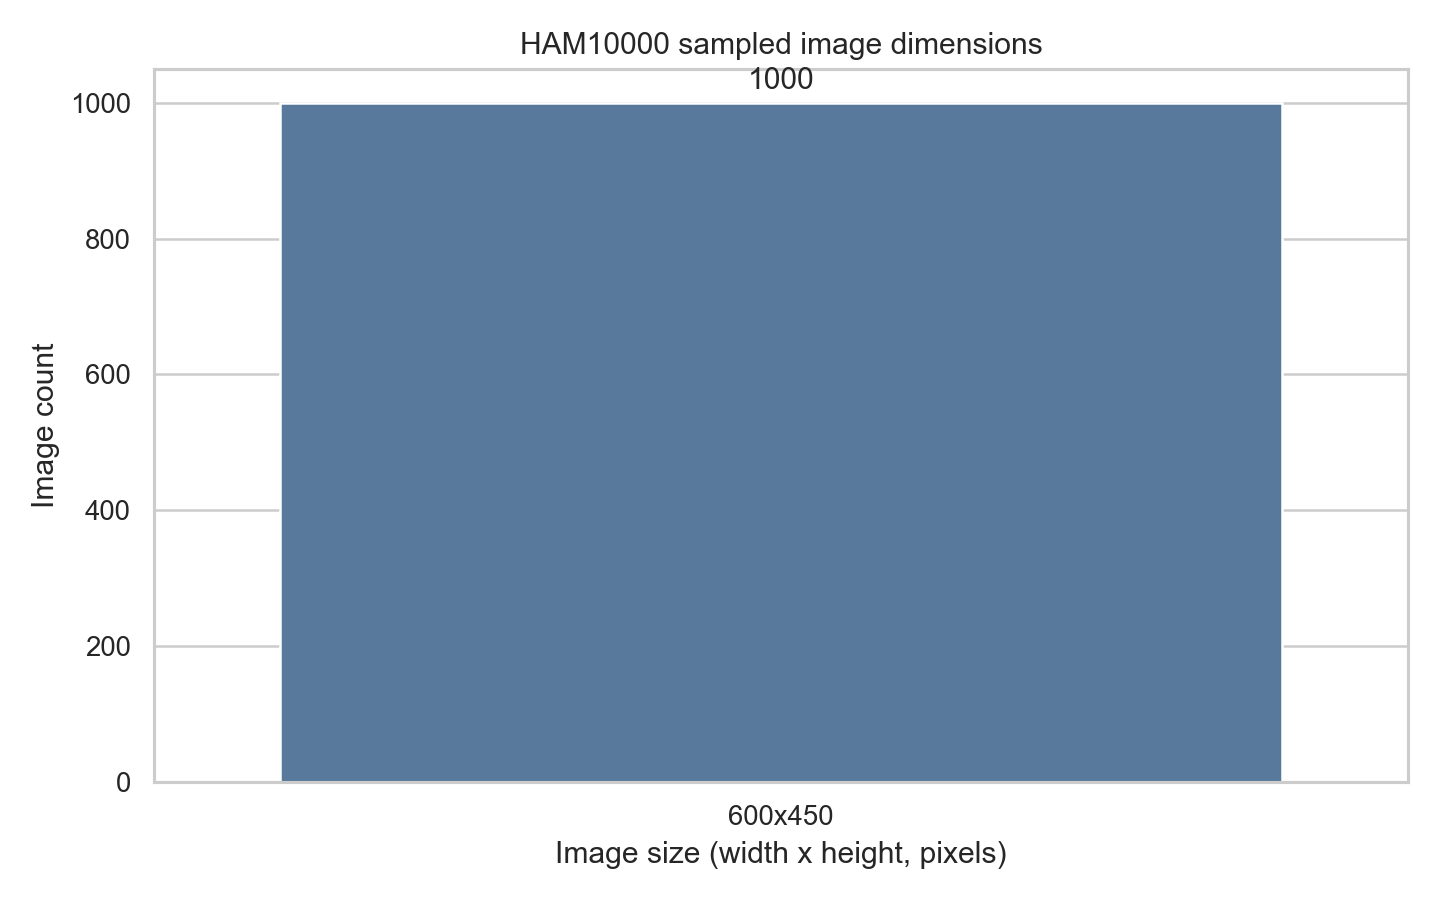
\includegraphics[width=0.94\textwidth]{images/ch3/ham10000_image_dimensions_histogram.png}
\caption[Histogram kích thước ảnh HAM10000]{Histogram kích thước ảnh HAM10000. Python source: \texttt{src/analyze\_ham10000.py}.}
\label{fig:ch4_ham_dimensions}
\end{figure}

\textbf{Nhận xét Hình \ref{fig:ch4_ham_dimensions}.} Kích thước ảnh gần như đồng nhất ở 600$\times$450, nên biến \texttt{width} và \texttt{height} chủ yếu dùng để xác nhận chất lượng dữ liệu đầu vào hơn là tạo thông tin phân biệt lớp.

\begin{figure}[H]
\centering
\includegraphics[width=0.94\textwidth]{images/ch3/ham10000_mean_intensity_boxplot.png}
\caption[Boxplot độ sáng theo lớp HAM10000]{Boxplot \texttt{mean\_intensity} theo lớp chẩn đoán HAM10000. Python source: \texttt{src/analyze\_ham10000.py}.}
\label{fig:ch4_ham_intensity}
\end{figure}

\textbf{Nhận xét Hình \ref{fig:ch4_ham_intensity}.} Boxplot độ sáng theo lớp cho thấy có chồng lấn lớn giữa các nhóm chẩn đoán. Vì vậy, đặc trưng thống kê ảnh đơn giản như \texttt{mean\_intensity} và \texttt{std\_intensity} chỉ nên xem là bước mô tả, không đủ thay thế đặc trưng màu/texture hoặc transfer learning.

\begin{figure}[H]
\centering
\includegraphics[width=0.94\textwidth]{images/ch3/ham10000_class_distribution.png}
\caption[Phân bố lớp \texttt{dx} HAM10000]{Phân bố lớp chẩn đoán \texttt{dx} trong HAM10000. Python source: \texttt{src/analyze\_ham10000.py}.}
\label{fig:ch4_ham_class_distribution}
\end{figure}

\textbf{Nhận xét Hình \ref{fig:ch4_ham_class_distribution}.} Phân bố lớp \texttt{dx} mất cân bằng mạnh, đặc biệt lớp \texttt{nv} chiếm tỷ trọng lớn. Vì vậy, accuracy có thể đánh lừa nếu mô hình chỉ dự đoán lớp phổ biến; khi đánh giá phân loại ảnh cần đọc thêm macro-F1, recall theo lớp và ma trận nhầm lẫn.

\begin{figure}[H]
\centering
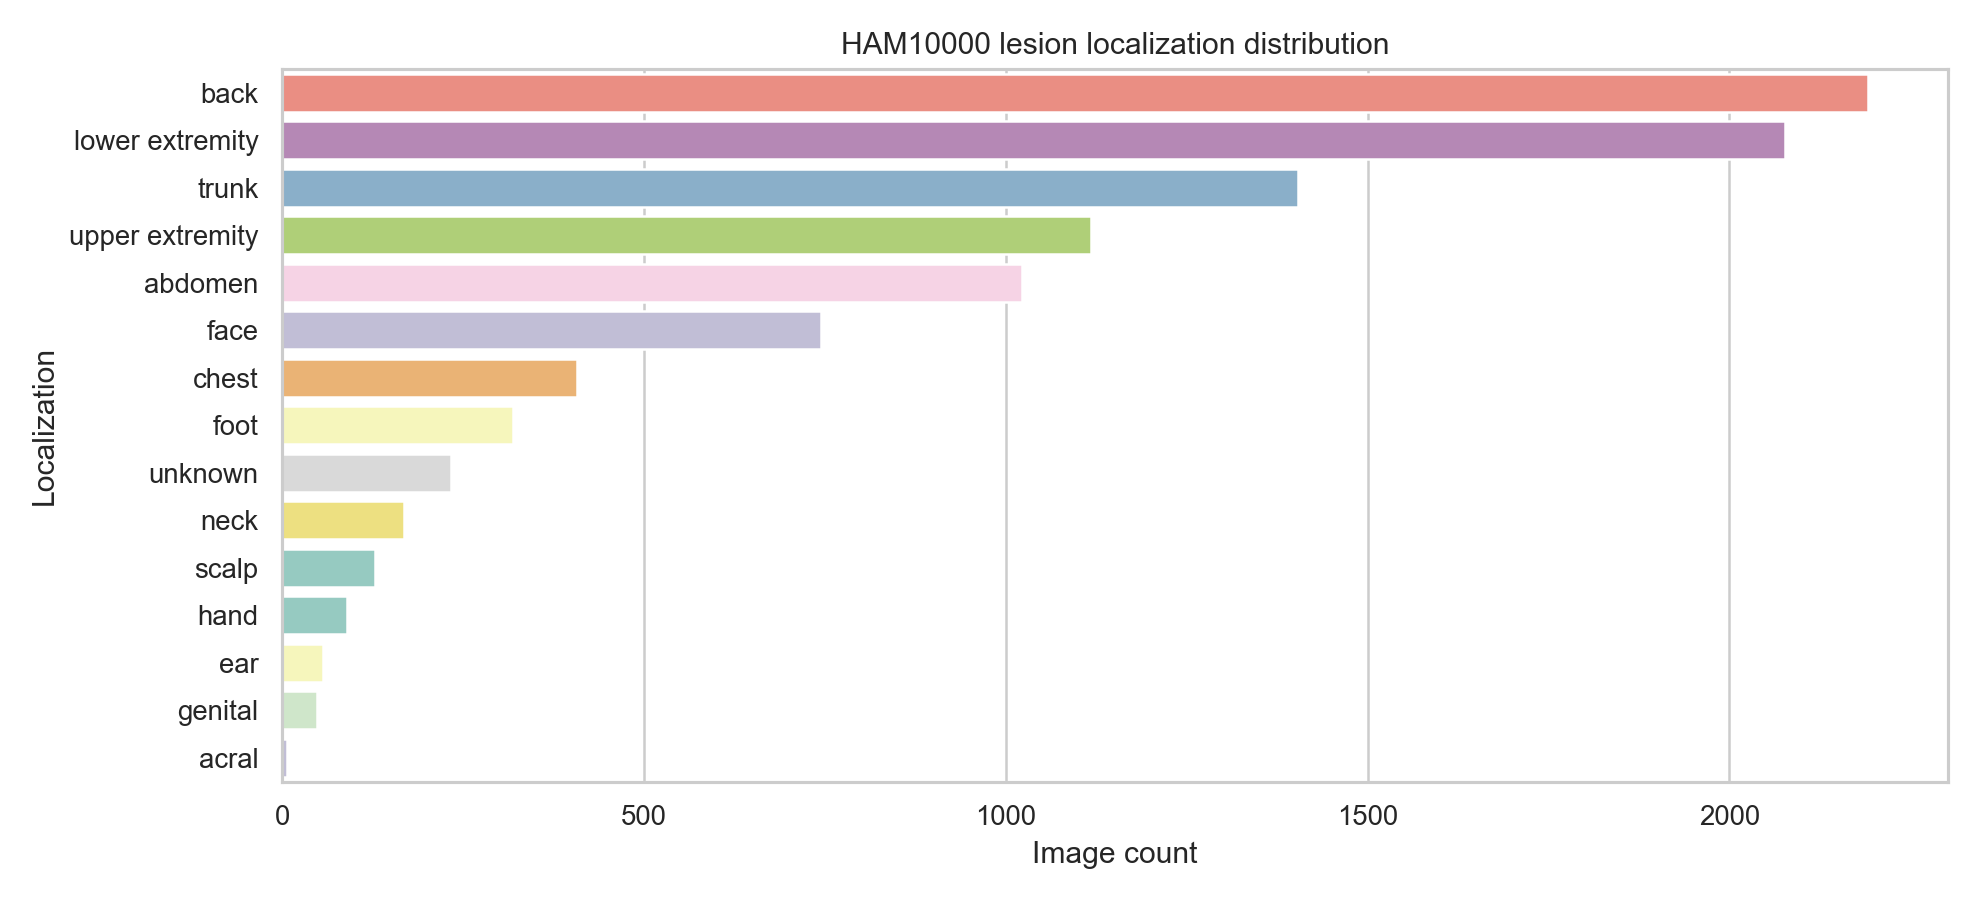
\includegraphics[width=0.94\textwidth]{images/ch3/ham10000_localization_bar.png}
\caption[Vị trí tổn thương HAM10000]{Tần suất vị trí tổn thương trong metadata HAM10000. Python source: \texttt{src/analyze\_ham10000.py}.}
\label{fig:ch4_ham_localization}
\end{figure}

\textbf{Nhận xét Hình \ref{fig:ch4_ham_localization}.} Biểu đồ vị trí tổn thương cho thấy một số vùng cơ thể xuất hiện nhiều hơn, nhưng vị trí không đủ để thay thế thông tin ảnh vì nhiều lớp bệnh có thể cùng xuất hiện ở một vùng.

\begin{figure}[H]
\centering
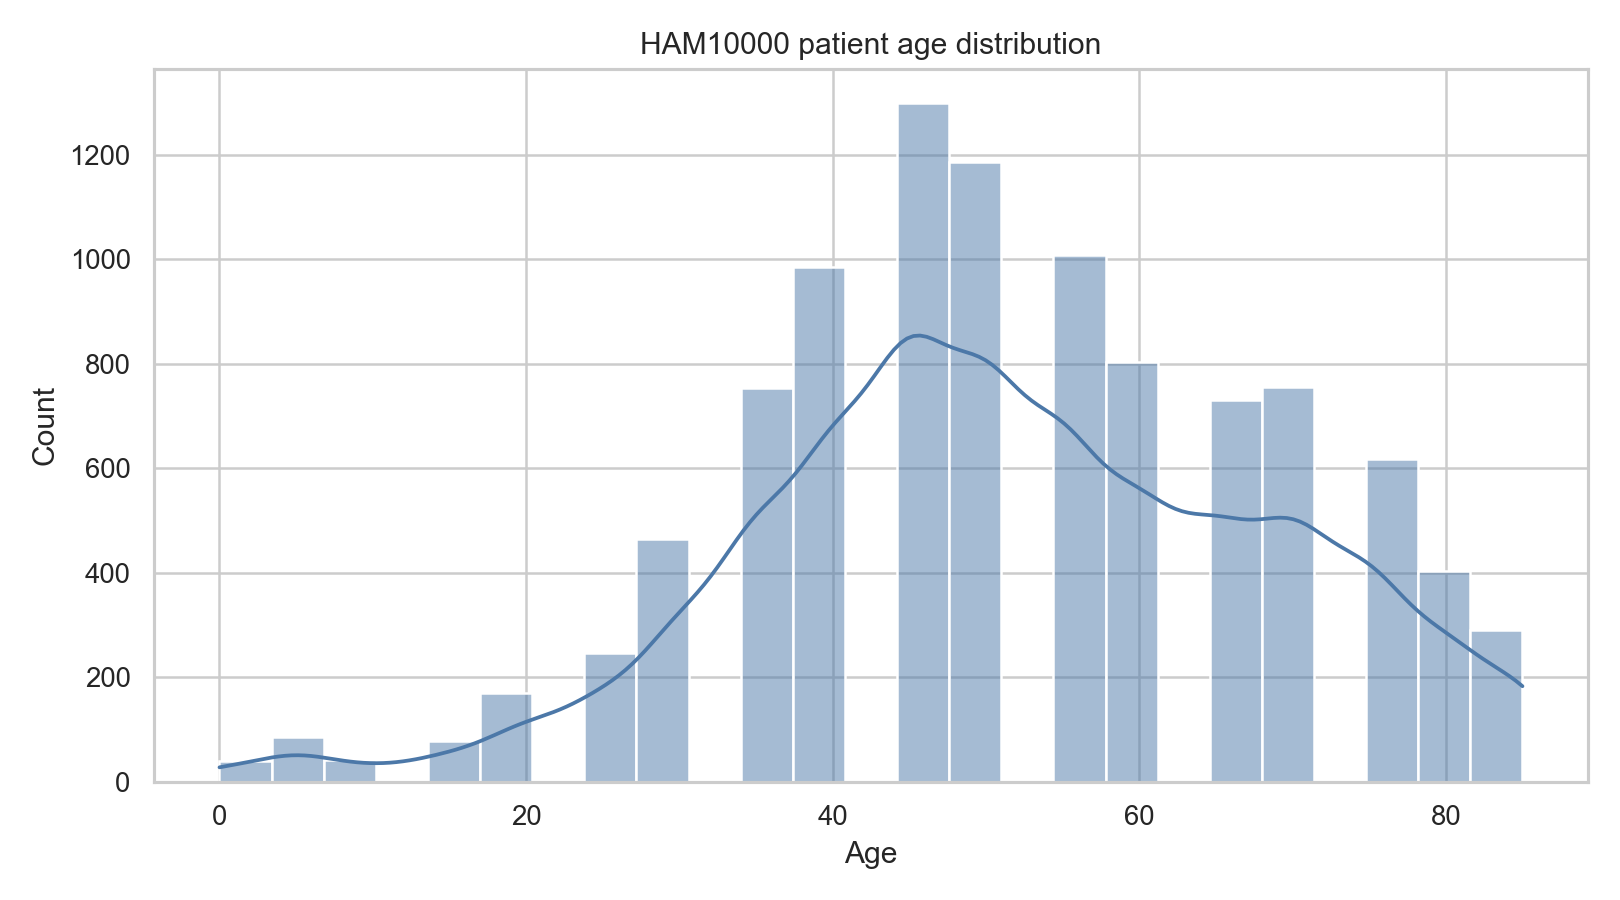
\includegraphics[width=0.78\textwidth]{images/ch3/ham10000_age_histogram.png}
\caption[Phân phối tuổi bệnh nhân HAM10000]{Phân phối tuổi bệnh nhân trong metadata HAM10000. Python source: \texttt{src/analyze\_ham10000.py}.}
\label{fig:ch4_ham_age}
\end{figure}

\textbf{Nhận xét Hình \ref{fig:ch4_ham_age}.} Histogram tuổi cho thấy mẫu HAM10000 tập trung nhiều ở nhóm trung niên và lớn tuổi, phù hợp với bối cảnh bệnh da liễu thường được ghi nhận nhiều hơn ở nhóm tuổi cao. Khi dùng metadata cho mô hình, tuổi có thể là biến hỗ trợ, nhưng không nên thay thế thông tin ảnh vì cùng một độ tuổi vẫn có thể xuất hiện nhiều lớp chẩn đoán khác nhau.

\textbf{Nhận xét tổng hợp HAM10000.} Kích thước ảnh đồng nhất ở 600$\times$450 nên không cần xử lý resize khi thống kê hình học. \texttt{mean\_intensity} dao động từ 93.88 đến 215.91, cho thấy sắc độ ảnh có đủ biến thiên để dùng làm đặc trưng mô tả. Tuy nhiên, các đặc trưng cường độ pixel đơn lẻ không đủ để phân loại ổn định, mà cần kết hợp đặc trưng sâu hoặc mô hình ảnh ở phần học máy.

\subsection{Bộ dữ liệu văn bản: Reuters-21578}

Reuters-21578 gồm 21\,578 văn bản tin tức. Văn bản được số hóa thành \texttt{word\_count}, \texttt{char\_count}, \texttt{primary\_topic} và danh sách topic đa nhãn. Các đặc trưng nâng cao như TF-IDF có thể dùng ở chương học máy, còn chương này tập trung vào thống kê độ dài và phân bố topic.

\begin{table}[H]
\centering
\caption{Phân loại biến số hóa từ Reuters-21578}
\label{tab:ch4_reuters_variable_types}
\small
\begin{tabularx}{\textwidth}{p{0.30\textwidth}p{0.32\textwidth}Y}
\toprule
Loại biến & Ví dụ & Ý nghĩa phân tích \\
\midrule
Quantitative Continuous & Điểm cảm xúc, mật độ stop words & Đặc trưng ngữ nghĩa mở rộng \\
Quantitative Discrete & \texttt{word\_count}, \texttt{char\_count}, số câu & Độ dài và độ phức tạp văn bản \\
Qualitative & \texttt{primary\_topic}, \texttt{topics}, ngôn ngữ & Nhãn phân loại chủ đề \\
\bottomrule
\end{tabularx}
\end{table}

\begin{table}[H]
\centering
\caption[Thống kê đặc trưng văn bản Reuters-21578]{Thống kê đặc trưng văn bản Reuters-21578. Source: \texttt{outputs/tables/reuters\_text\_summary.csv}.}
\label{tab:ch4_reuters_stats}
\small
\begin{tabular}{lrrrrrrrr}
\toprule
Biến & Mean & Median & Std & Min & Max & CV & IQR & n \\
\midrule
\texttt{word\_count} & 132.86 & 93.00 & 139.70 & 0 & 2\,381 & 1.051 & 111 & 21\,578 \\
\texttt{char\_count} & 762.06 & 534.00 & 819.74 & 0 & 9\,910 & 1.076 & 672 & 21\,578 \\
\bottomrule
\end{tabular}
\end{table}

\begin{figure}[H]
\centering
\begin{subfigure}{0.48\textwidth}
 \centering
 \includegraphics[width=\textwidth]{images/ch3/reuters_word_count_histogram.png}
 \caption{Histogram số từ}
\end{subfigure}
\hfill
\begin{subfigure}{0.48\textwidth}
 \centering
 \includegraphics[width=\textwidth]{images/ch3/reuters_top_topics.png}
 \caption{Top topic}
\end{subfigure}
\caption[Số hóa văn bản Reuters-21578]{Số hóa và trực quan hóa văn bản Reuters-21578. Python source: \texttt{src/analyze\_reuters.py}.}
\label{fig:ch4_reuters_dataset}
\end{figure}

\textbf{Nhận xét Hình \ref{fig:ch4_reuters_dataset}.} Histogram \texttt{word\_count} cho thấy phân phối lệch phải rất mạnh: đa số tin ngắn, một số ít tin rất dài. Biểu đồ top topic cho thấy \texttt{earn} và \texttt{acq} chiếm ưu thế, trong khi nhiều topic chuyên ngành có ít mẫu; khi dùng Reuters cho phân loại văn bản, macro-F1 sẽ có ý nghĩa hơn accuracy vì phản ánh tốt hơn hiệu năng trên các lớp nhỏ.

\begin{figure}[H]
\centering
\begin{subfigure}{0.48\textwidth}
 \centering
 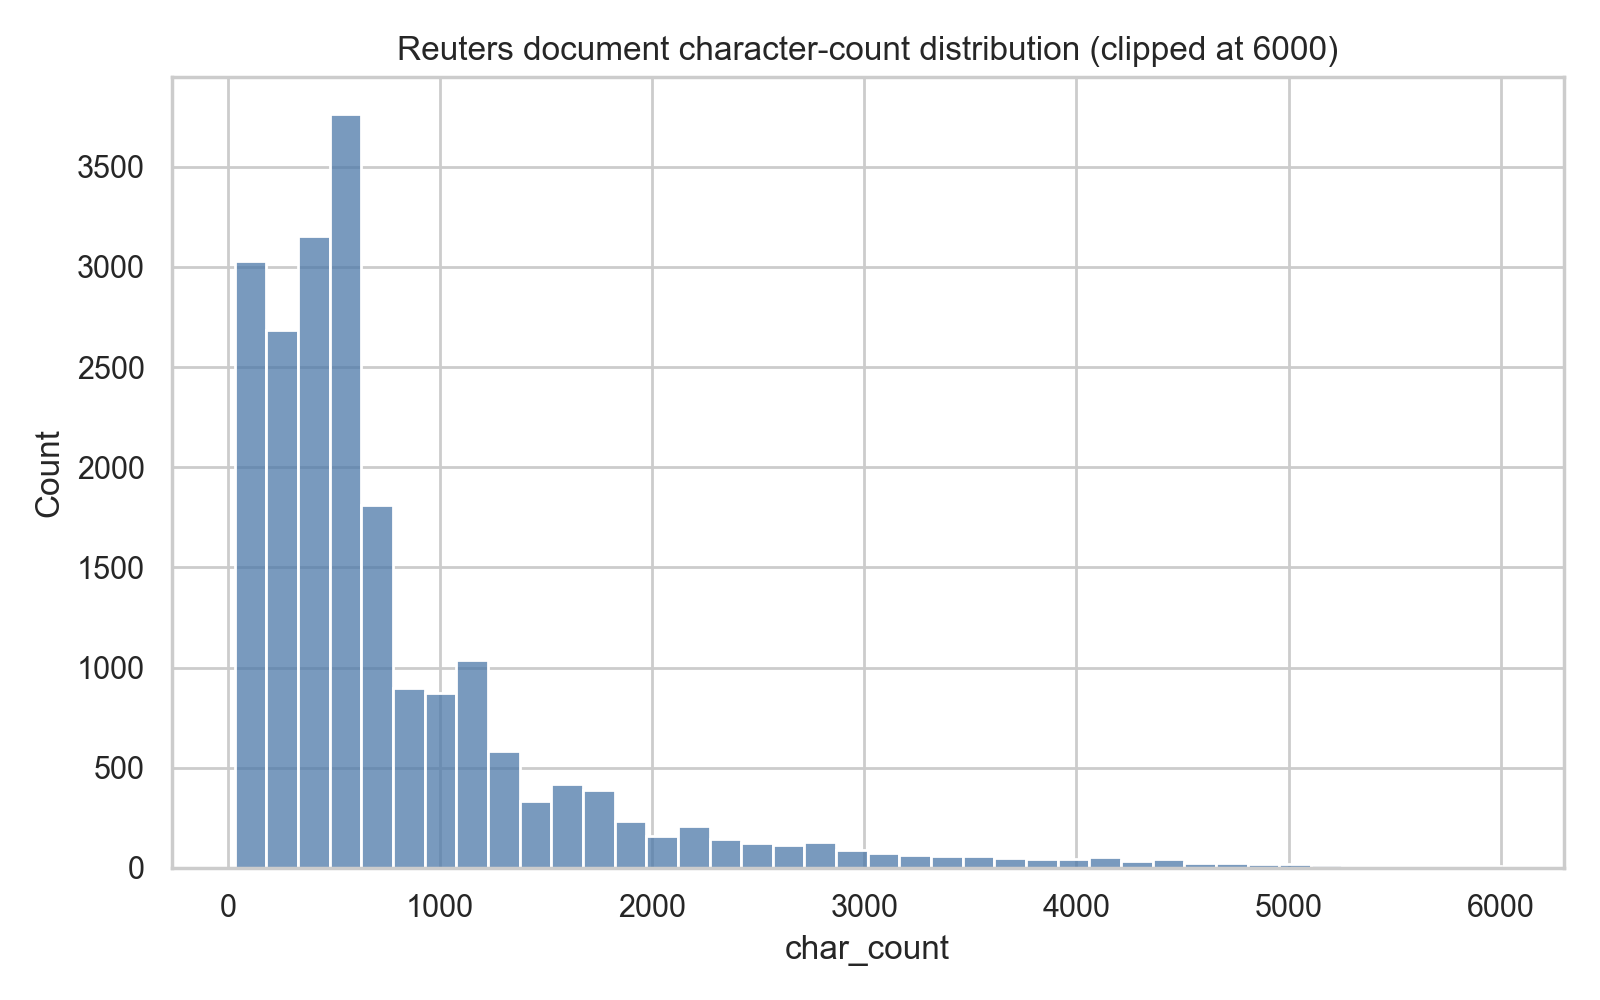
\includegraphics[width=\textwidth]{images/ch3/reuters_char_count_histogram.png}
 \caption{Histogram số ký tự}
\end{subfigure}
\hfill
\begin{subfigure}{0.48\textwidth}
 \centering
 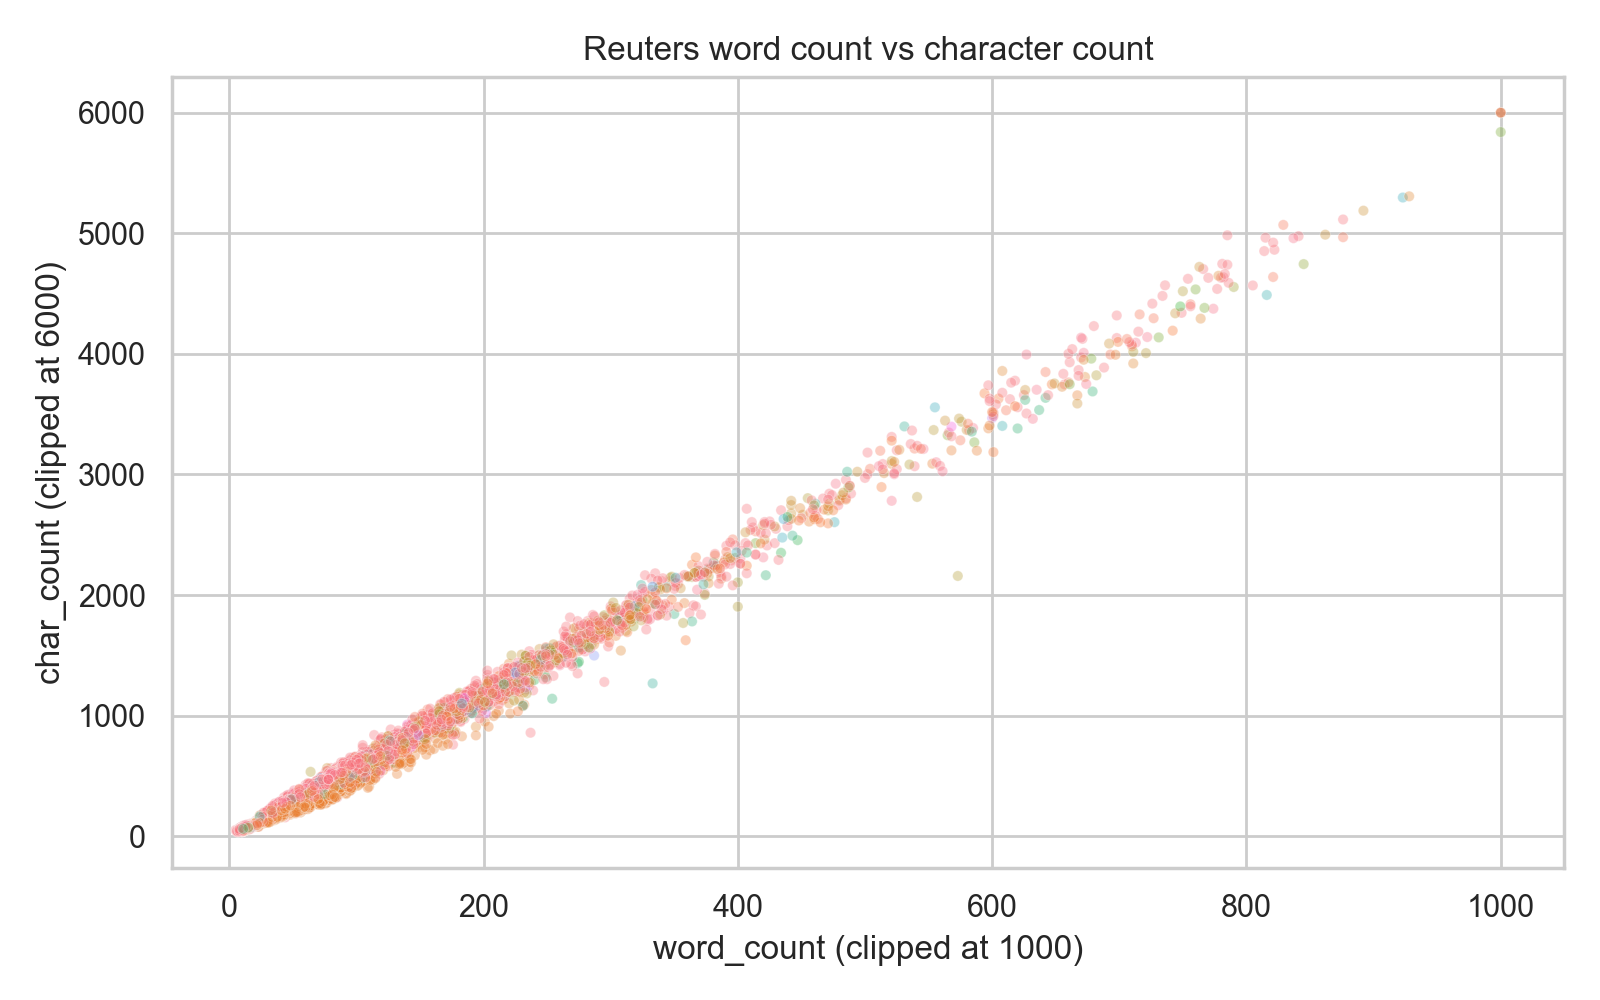
\includegraphics[width=\textwidth]{images/ch3/reuters_word_char_scatter.png}
 \caption{Scatter số từ--số ký tự}
\end{subfigure}
\caption[Phân tích độ dài văn bản Reuters-21578]{Phân tích độ dài văn bản Reuters-21578 theo số ký tự và quan hệ số từ--số ký tự. Python source: \texttt{src/analyze\_reuters.py}.}
\label{fig:ch4_reuters_length}
\end{figure}

\textbf{Nhận xét Hình \ref{fig:ch4_reuters_length}.} Histogram số ký tự xác nhận kết luận từ \texttt{word\_count}: phần lớn bản tin ngắn, nhưng vẫn có đuôi phải gồm các văn bản dài. Scatter số từ--số ký tự gần như tạo thành một dải tuyến tính, nghĩa là hai đặc trưng độ dài chứa thông tin trùng lặp đáng kể; khi xây dựng mô hình, nên chuẩn hóa hoặc chọn một đại diện độ dài để tránh làm mô hình quá thiên về kích thước văn bản thay vì nội dung.

\section{Kết luận chương}

Chương này đã triển khai đầy đủ yêu cầu thống kê và trực quan hóa trên ba nhóm dữ liệu. Với nhóm A, Heart Disease cho thấy vai trò của phân loại biến và xử lý ngoại lai; CDC Diabetes nhấn mạnh dữ liệu lớn, biến thứ bậc và mất cân bằng lớp; Breast Cancer thể hiện các biến Quantitative có lực phân tách rõ. Với nhóm B, Appliances Energy chứng minh cần đọc xu hướng bằng line chart và dùng log-transform cho phân phối lệch phải; HAR/MHEALTH cho thấy dữ liệu cảm biến cần chuẩn hóa trước khi tính khoảng cách hoặc gom cụm. Với nhóm C, HAM10000 và Reuters-21578 chứng minh nguyên tắc số hóa dữ liệu đa phương tiện thành đặc trưng Quantitative trước khi thống kê.

Các kết quả này là nền tảng trực tiếp cho chương học máy: phân loại nhóm A phải chú ý mất cân bằng và ngoại lai; dự báo nhóm B phải tách theo thời gian; gom cụm nhóm A/B/C phải chuẩn hóa đặc trưng và ẩn nhãn trước khi đánh giá cấu trúc tự nhiên của dữ liệu.

\chapter{PHÂN TÍCH DỮ LIỆU VỚI HỌC MÁY VÀ ĐỐI SÁNH KẾT QUẢ}
\label{ch:chuong5}

\startcontents[chapters]
\printmyminitoc{
Chương này sử dụng trực tiếp các phiên bản dữ liệu đã làm sạch ở Chương 4 (mục 4.1, 4.3) làm đầu vào cho ba bài toán học máy kinh điển: phân lớp (Classification) trên dữ liệu Nhóm A, hồi quy chuỗi thời gian (Regression) trên dữ liệu Nhóm B, và gom cụm (Clustering) không giám sát trên cả ba nhóm dữ liệu A, B, C. Mục tiêu không chỉ là tối ưu chỉ số hiệu năng mà còn diễn giải ý nghĩa thực tế của kết quả, đặc biệt là ảnh hưởng của các đặc điểm dữ liệu đã phát hiện ở Chương 4 (mất cân bằng lớp, outlier, tính mùa vụ...) lên hành vi của mô hình.}

\section{Môi trường cài đặt và cách đánh giá}

\subsection{Thiết lập môi trường thực nghiệm}

Toàn bộ thực nghiệm được cài đặt bằng \textbf{Python 3}, sử dụng các thư viện chính: \texttt{pandas}/\texttt{numpy} (xử lý dữ liệu), \texttt{scikit-learn} (Logistic Regression, Random Forest, SVM, KMeans, Agglomerative Clustering, Gaussian Mixture, các độ đo đánh giá và \texttt{StandardScaler}), \texttt{statsmodels} (ARIMA), \texttt{xgboost} (XGBoost Regressor), \texttt{matplotlib}/\texttt{seaborn} (trực quan hóa kết quả). Dữ liệu đầu vào là các phiên bản \textbf{đã làm sạch} (đã điền khuyết, xử lý outlier) được xuất ra từ Chương 4, đảm bảo tính nhất quán giữa bước phân tích khám phá dữ liệu và bước huấn luyện mô hình.

Quy trình thực nghiệm được tổ chức thành 5 script độc lập, tương ứng với từng bước của pipeline:
\begin{itemize}
    \item \texttt{step1\_classification.py} -- huấn luyện và đánh giá 3 thuật toán phân lớp trên 3 bộ dữ liệu Nhóm A;
    \item \texttt{step2\_confusion\_and\_imbalance.py} -- dựng ma trận nhầm lẫn và phân tích chuyên sâu vấn đề mất cân bằng lớp trên CDC Diabetes;
    \item \texttt{step3\_regression.py} -- huấn luyện 3 mô hình dự báo chuỗi thời gian trên Appliances Energy;
    \item \texttt{step4\_regression\_charts.py} -- dựng các biểu đồ phân tích dự báo (forecast, residual, feature importance);
    \item \texttt{step5\_clustering.py} -- thực hiện gom cụm không giám sát trên 3 bộ dữ liệu đại diện Nhóm A/B/C.
\end{itemize}

\subsection{Các độ đo đánh giá}

Đối với bài toán \textbf{phân lớp} (mục~\ref{sec:classification}), các độ đo được sử dụng gồm Accuracy, Precision, Recall và F1-Score (tính theo kiểu binary cho bài toán 2 lớp, và macro-average cho bài toán 3 lớp CDC Diabetes để tránh chỉ số bị chi phối bởi lớp đa số):

\begin{equation}\label{eq:acc}
Accuracy = \frac{TP+TN}{TP+TN+FP+FN}
\end{equation}

\begin{equation}
Precision = \frac{TP}{TP+FP}
\end{equation}

\begin{equation}
Recall = \frac{TP}{TP+FN}
\end{equation}

\begin{equation}
F1 = \frac{2 \times Precision \times Recall}{Precision+Recall} = \frac{2 \times TP}{2 \times TP+FP+FN}
\end{equation}

Đối với bài toán \textbf{hồi quy} (mục~\ref{sec:regression}), sử dụng MAE (Mean Absolute Error), RMSE (Root Mean Squared Error) và MAPE (Mean Absolute Percentage Error):

\begin{equation}
MAE = \frac{1}{n}\sum_{i=1}^{n}|y_i - \hat{y}_i\,|, \quad
RMSE = \sqrt{\frac{1}{n}\sum_{i=1}^{n}(y_i - \hat{y}_i)^2}, \quad
MAPE = \frac{100\%}{n}\sum_{i=1}^{n}\left|\frac{y_i - \hat{y}_i}{y_i}\right|
\end{equation}

Đối với bài toán \textbf{gom cụm} (mục~\ref{sec:clustering}), sử dụng Silhouette Score (đo mức độ tách biệt giữa các cụm, dao động từ $-1$ đến $1$, càng gần 1 càng tốt) làm tiêu chí chính để chọn số cụm $K$ tối ưu và so sánh giữa các giải thuật.


\section{Bài toán dự đoán phân lớp (Classification) trên Data A}
\label{sec:classification}

Ba bộ dữ liệu Nhóm A đã được làm sạch ở Chương 4 được sử dụng làm ba bài toán phân lớp độc lập, mỗi bài toán ứng với một biến mục tiêu (target) khác nhau:
\begin{itemize}
    \item \textbf{Target 1 -- Breast Cancer Wisconsin}: phân lớp nhị phân \texttt{diagnosis} (Benign/Malignant), dữ liệu đầu vào là 6 đặc trưng hình thái đã làm sạch ở mục 4.1.1 (569 mẫu);
    \item \textbf{Target 2 -- Heart Disease (Cleveland)}: phân lớp nhị phân \texttt{target} (Có/Không bệnh tim), 13 đặc trưng lâm sàng đã làm sạch ở mục 4.1.2 (303 mẫu);
    \item \textbf{Target 3 -- CDC Diabetes Health Indicators}: phân lớp \textbf{3 mức} \texttt{Diabetes\_012} (Không tiểu đường/Tiền tiểu đường/Tiểu đường), 21 đặc trưng đã làm sạch ở mục 4.1.3.
\end{itemize}

\subsection{Quy trình thực nghiệm}

Quy trình áp dụng thống nhất cho cả 3 bộ dữ liệu:
\begin{enumerate}
    \item \textbf{Chia tách Train/Test}: tỉ lệ 80/20, sử dụng \texttt{stratify} theo biến mục tiêu để đảm bảo tỉ lệ các lớp trong tập train và test tương đồng với tỉ lệ gốc -- đặc biệt quan trọng với bộ CDC Diabetes vốn đã mất cân bằng lớp nghiêm trọng (Chương 4, mục 4.1.3).
    \item \textbf{Chuẩn hóa dữ liệu}: áp dụng \texttt{StandardScaler} (đưa về trung bình 0, phương sai 1) cho Logistic Regression và SVM (2 thuật toán nhạy cảm với thang đo); Random Forest giữ nguyên dữ liệu gốc vì thuật toán dựa trên cây quyết định không yêu cầu chuẩn hóa.
    \item \textbf{Xử lý mất cân bằng lớp}: tham số \texttt{class\_weight="balanced"} được kích hoạt cho Random Forest và SVM, tự động tăng trọng số cho các lớp thiểu số trong hàm mất mát.
    \item \textbf{Riêng bộ CDC Diabetes} (253.680 mẫu): do kích thước quá lớn khiến SVM không khả thi về thời gian huấn luyện, nhóm lấy mẫu ngẫu nhiên phân tầng (stratified subsample) 30.000 dòng (giữ nguyên tỉ lệ 3 lớp gốc) trước khi chia Train/Test, một điều chỉnh thực tế thường gặp khi triển khai SVM trên dữ liệu lớn.
\end{enumerate}

Ba thuật toán được so sánh: \textbf{Logistic Regression} (mô hình tuyến tính, dễ diễn giải), \textbf{Random Forest} (200 cây, tổ hợp phi tuyến, mạnh với dữ liệu hỗn hợp), \textbf{SVM kernel RBF} (biên phân lớp phi tuyến, tốt với dữ liệu đã chuẩn hóa).

\subsection{Bảng so sánh hiệu năng các thuật toán}

\begin{table}[H]
\centering
\caption{So sánh hiệu năng 3 thuật toán trên 3 bộ dữ liệu (Precision/Recall/F1: binary cho Breast Cancer và Heart Disease, macro-average cho CDC Diabetes 3 lớp)}
\label{tab:classification-results}
\label{tab:chapter4_classification_metrics}
\begin{tabular}{llcccc}
\toprule
\textbf{Dataset} & \textbf{Mô hình} & \textbf{Accuracy} & \textbf{Precision} & \textbf{Recall} & \textbf{F1-Score} \\
\midrule
\multirow{3}{*}{Breast Cancer (n\_test=114)} & Logistic Regression & 0,9035 & 0,8780 & 0,8571 & 0,8675 \\
 & Random Forest & 0,9123 & 0,9000 & 0,8571 & 0,8780 \\
 & SVM (RBF) & \textbf{0,9211} & 0,8667 & \textbf{0,9286} & \textbf{0,8966} \\
\midrule
\multirow{3}{*}{Heart Disease (n\_test=61)} & Logistic Regression & 0,8689 & 0,8125 & 0,9286 & 0,8667 \\
 & Random Forest & \textbf{0,9016} & \textbf{0,8438} & 0,9643 & \textbf{0,9000} \\
 & SVM (RBF) & 0,8852 & 0,8182 & \textbf{0,9643} & 0,8852 \\
\midrule
\multirow{3}{*}{CDC Diabetes (n\_test=6000)} & Logistic Regression & \textbf{0,8472} & \textbf{0,4626} & 0,3845 & 0,3937 \\
 & Random Forest & 0,8438 & 0,4561 & 0,3662 & 0,3679 \\
 & SVM (RBF) & 0,6523 & 0,4290 & \textbf{0,4823} & \textbf{0,4154} \\
\bottomrule
\end{tabular}
\end{table}

Nhận xét tổng quan: SVM (RBF) cho kết quả tốt nhất trên bộ Breast Cancer (F1=0,8966) -- phù hợp vì dữ liệu chỉ có 6 đặc trưng liên tục, ranh giới phân lớp phi tuyến nhẹ mà kernel RBF xử lý hiệu quả. Random Forest vượt trội trên bộ Heart Disease (F1=0,9000) nhờ khả năng nắm bắt tương tác giữa các đặc trưng hỗn hợp (định lượng + định tính mã hóa). Đáng chú ý, trên bộ CDC Diabetes, \textbf{Accuracy cao nhất (Logistic Regression, 84,72\%) lại đi kèm F1-macro thấp nhất trong nhóm cạnh tranh} (chỉ nhỉnh hơn Random Forest) -- đây chính là dấu hiệu kinh điển của bài toán mất cân bằng lớp, được phân tích chi tiết ở mục~\ref{sec:imbalance-discussion}.

\subsection{Phân tích ma trận nhầm lẫn}

\begin{figure}[H]
    \centering
    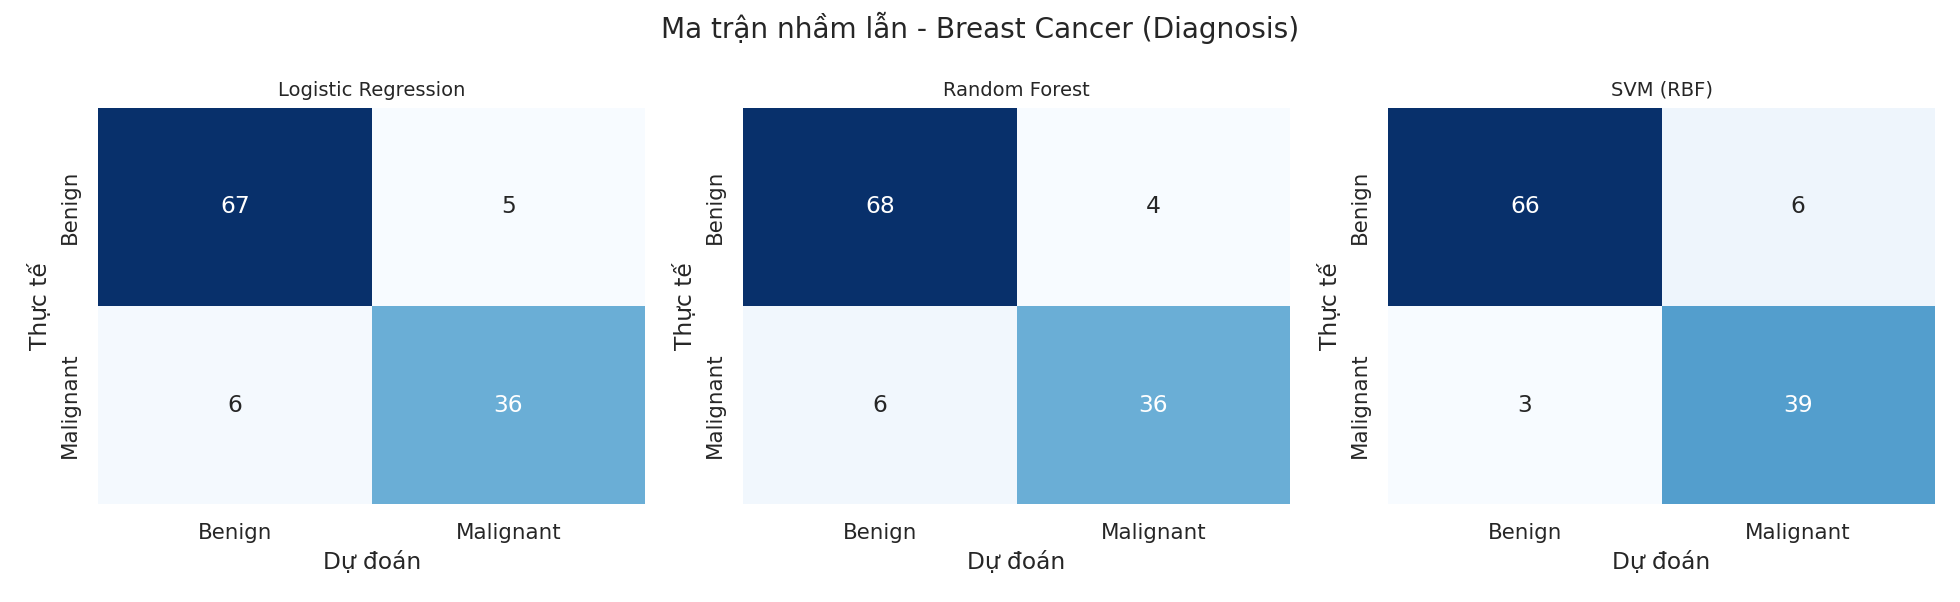
\includegraphics[width=\textwidth]{images/ch4_ml/fig1_cm_breastcancer.png}
    \caption{Ma trận nhầm lẫn - Breast Cancer (Diagnosis)}
    \label{fig:cm-bc}
\end{figure}

Nhận xét: Cả 3 mô hình đều có số lượng \textit{False Negative} (dự đoán Benign nhưng thực tế Malignant) rất thấp (0--3 ca trên 114 mẫu test) -- đây là điểm quan trọng về mặt lâm sàng, vì bỏ sót ca ác tính (False Negative) nguy hiểm hơn nhiều so với báo động giả (False Positive). SVM có ít False Negative nhất (Recall cao nhất), phù hợp mục tiêu ưu tiên trong sàng lọc y tế.

\begin{figure}[H]
    \centering
    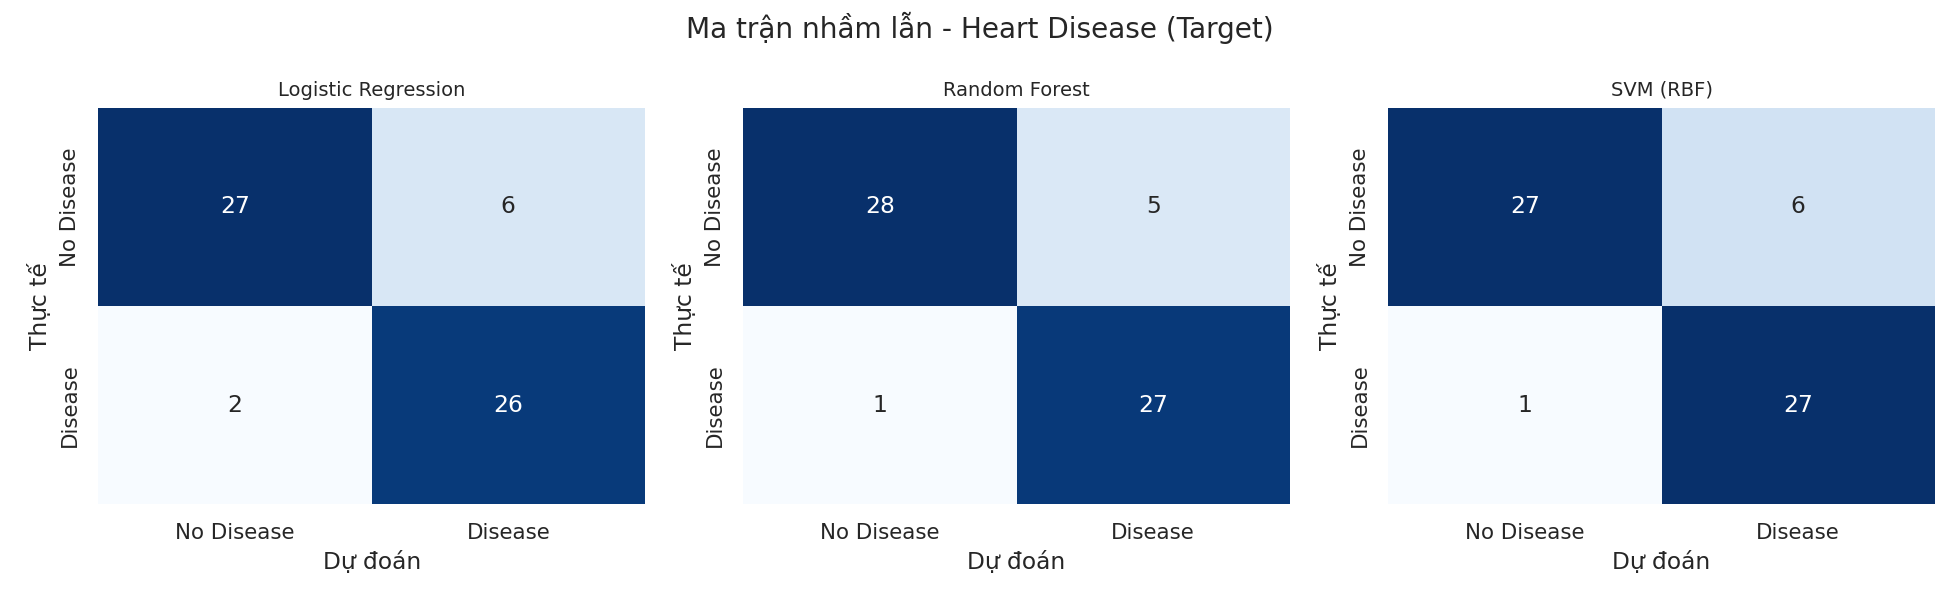
\includegraphics[width=\textwidth]{images/ch4_ml/fig2_cm_heart.png}
    \caption{Ma trận nhầm lẫn - Heart Disease (Target)}
    \label{fig:cm-heart}
\end{figure}

Nhận xét: Random Forest và SVM đều đạt Recall rất cao (0,9643, chỉ bỏ sót 1/28 ca bệnh thật trong tập test), nhất quán với đặc điểm đã phát hiện ở Chương 4 rằng \texttt{thalach} và \texttt{oldpeak} là các đặc trưng phân tách tốt giữa 2 lớp.

\begin{figure}[H]
    \centering
    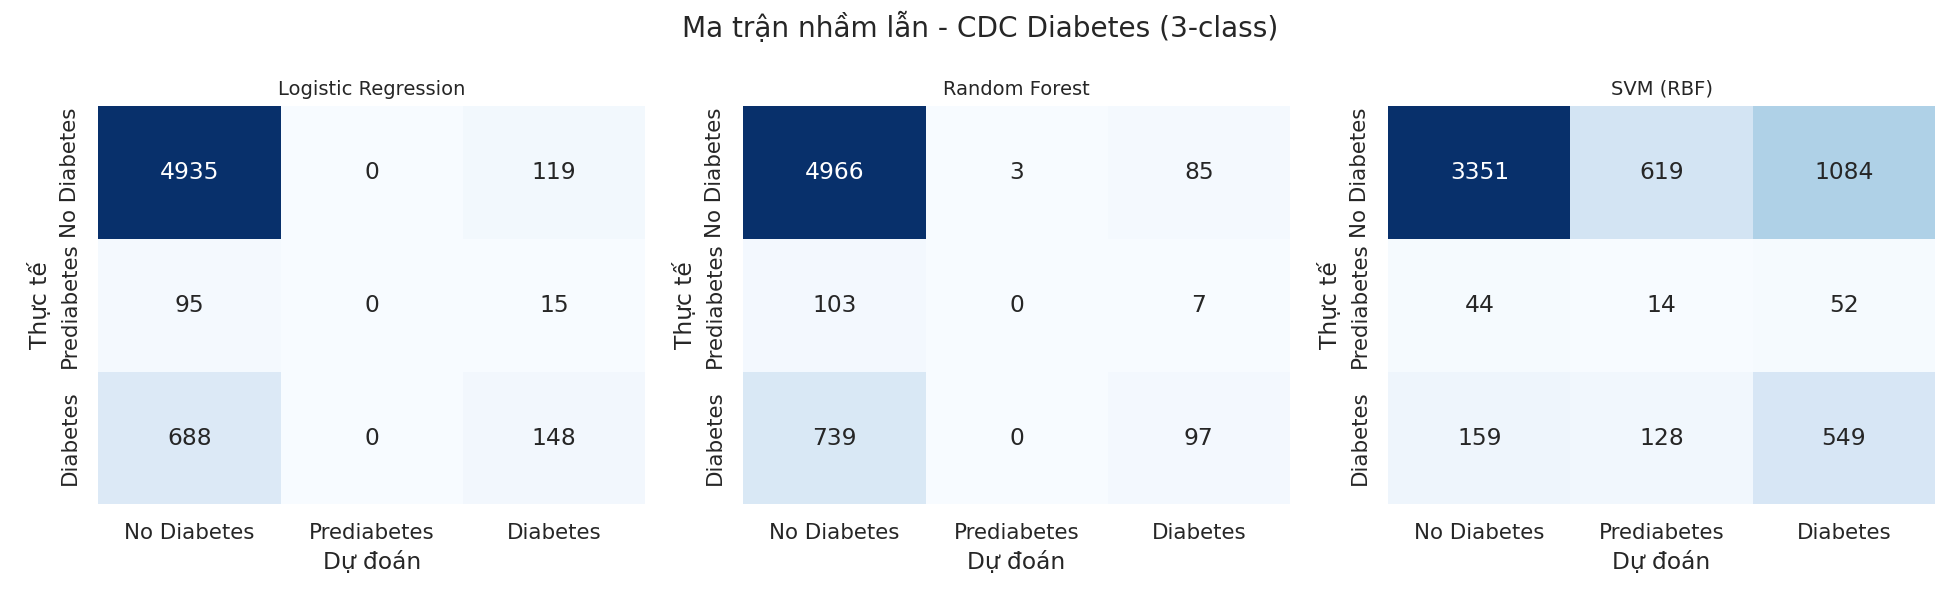
\includegraphics[width=\textwidth]{images/ch4_ml/fig3_cm_diabetes.png}
    \caption{Ma trận nhầm lẫn - CDC Diabetes (3 lớp)}
    \label{fig:cm-diabetes}
    \label{fig:chapter4_classification_confusion}
\end{figure}

Nhận xét: Ma trận nhầm lẫn của cả 3 mô hình đều lộ rõ vấn đề nghiêm trọng ở lớp \textbf{Tiền tiểu đường (Prediabetes)} -- hầu hết các mẫu thuộc lớp này bị dự đoán nhầm sang lớp Không tiểu đường hoặc Tiểu đường, gần như không có ca nào được dự đoán đúng, được lượng hóa chi tiết ở mục dưới đây.

\subsection{Nhận xét chuyên sâu về bài toán dữ liệu mất cân bằng}
\label{sec:imbalance-discussion}

Bộ CDC Diabetes có tỉ lệ 3 lớp cực kỳ lệch (84,24\% / 1,83\% / 13,93\% -- đã phân tích ở Chương 4, mục 4.1.3). Bảng~\ref{tab:diabetes-perclass} lượng hóa Recall theo từng lớp riêng biệt của mô hình Random Forest, cho thấy rõ hệ quả của mất cân bằng lớp mà chỉ số Accuracy tổng thể (84,38\%) hoàn toàn che giấu.

\begin{table}[H]
\centering
\caption{Recall theo từng lớp - CDC Diabetes (Random Forest)}
\label{tab:diabetes-perclass}
\begin{tabular}{lcc}
\toprule
\textbf{Lớp} & \textbf{Số mẫu test} & \textbf{Recall} \\
\midrule
Không tiểu đường & 5.054 & 0,9826 \\
Tiền tiểu đường & 110 & \textbf{0,0000} \\
Tiểu đường & 836 & 0,1160 \\
\bottomrule
\end{tabular}
\end{table}

\begin{figure}[H]
    \centering
    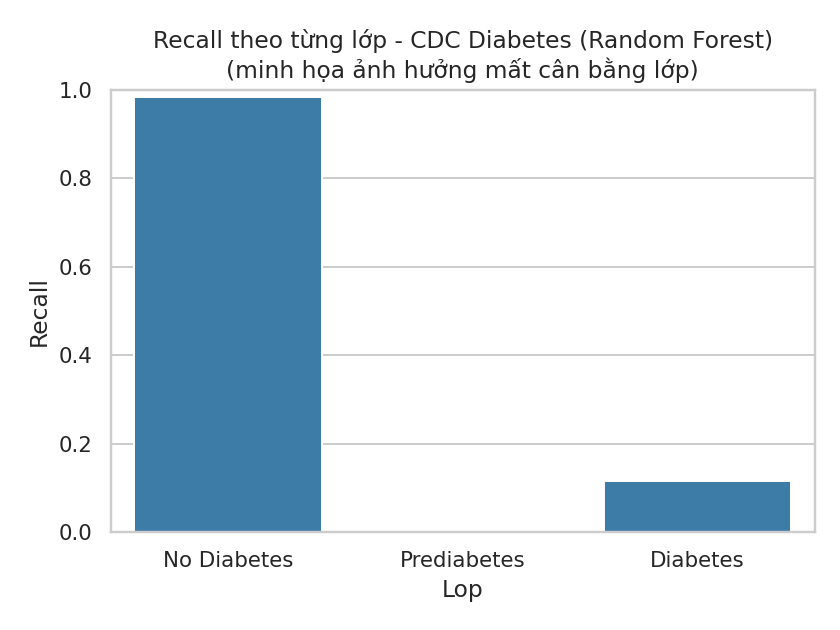
\includegraphics[width=0.6\textwidth]{images/ch4_ml/fig4_perclass_recall_diabetes.png}
    \caption{Recall theo từng lớp - CDC Diabetes (Random Forest)}
    \label{fig:perclass-recall}
\end{figure}

\textbf{Nhận xét, biện luận:}
\begin{itemize}
    \item \textbf{Lớp Tiền tiểu đường có Recall = 0,0000} -- mô hình không nhận diện đúng \textit{bất kỳ} ca nào trong 110 ca thuộc lớp này ở tập test, mặc dù đã áp dụng \texttt{class\_weight="balanced"}. Nguyên nhân: lớp này chỉ chiếm 1,83\% dữ liệu gốc, và về mặt lâm sàng, "tiền tiểu đường" là trạng thái trung gian có đặc trưng chồng lấn cao với cả hai lớp còn lại (các chỉ số BMI, GenHlth ở mức "gần ranh giới"), khiến mô hình có xu hướng phân loại vào 1 trong 2 lớp phổ biến hơn thay vì lớp hiếm ở giữa.
    \item \textbf{Nghịch lý Accuracy cao nhưng F1-macro thấp}: Accuracy 84,38\% chủ yếu đến từ việc dự đoán đúng lớp đa số (Không tiểu đường, Recall 98,26\%) -- nếu một mô hình "ngu" luôn dự đoán "Không tiểu đường" cho mọi trường hợp, Accuracy vẫn đạt khoảng 84\% (bằng đúng tỉ lệ lớp này trong dữ liệu), nhưng hoàn toàn vô dụng về mặt thực tiễn. Đây là lý do \textbf{Accuracy là chỉ số không đáng tin cậy trên dữ liệu mất cân bằng}, và F1-macro (coi trọng đều cả 3 lớp bất kể tần suất) là thước đo phù hợp hơn để đánh giá mô hình trong bài toán này.
    \item \textbf{So sánh giữa 3 mô hình}: SVM có F1-macro cao nhất (0,4154) dù Accuracy thấp nhất (65,23\%) -- SVM với \texttt{class\_weight="balanced"} chấp nhận hy sinh độ chính xác trên lớp đa số để cải thiện Recall các lớp thiểu số (Recall tổng macro 0,4823, cao nhất trong 3 mô hình), một sự đánh đổi (trade-off) kinh điển giữa Accuracy và khả năng phát hiện lớp hiếm.
    \item \textbf{Khuyến nghị cải thiện}: để giải quyết triệt để vấn đề này, cần áp dụng thêm các kỹ thuật resampling chuyên biệt như SMOTE (Synthetic Minority Oversampling) cho riêng lớp Tiền tiểu đường, hoặc gộp bài toán về nhị phân (có nguy cơ / không có nguy cơ tiểu đường) nếu mục tiêu ứng dụng thực tế không yêu cầu phân biệt chi tiết giai đoạn tiền tiểu đường.
\end{itemize}

\section{Bài toán dự đoán hồi quy (Regression) trên Data B}
\label{sec:regression}

Bộ dữ liệu Appliances Energy Prediction (đã làm sạch ở Chương 4, mục 4.1.4) được sử dụng cho bài toán dự báo giá trị tiêu thụ điện năng \texttt{Appliances} trong tương lai. Để bài toán dự báo có ý nghĩa thực tiễn hơn (thay vì dự báo từng điểm 10 phút quá nhiễu), nhóm resample dữ liệu về \textbf{tần suất theo giờ} (trung bình mỗi giờ), thu được 3.290 điểm dữ liệu liên tục từ 12/01/2016 đến 27/05/2016.

\subsection{Xây dựng đặc trưng và chia dữ liệu theo Time Series Split}

Các đặc trưng đầu vào được xây dựng dựa trên phát hiện về tính mùa vụ đã phân tích ở Chương 4 (mục 4.1.4):
\begin{itemize}
    \item \texttt{hour}, \texttt{dayofweek}, \texttt{is\_weekend} -- đặc trưng thời gian nắm bắt mùa vụ trong ngày/tuần;
    \item \texttt{lag\_1} (giá trị giờ liền trước), \texttt{lag\_24} (giá trị cùng giờ ngày hôm trước), \texttt{rolling\_mean\_24} (trung bình trượt 24 giờ) -- đặc trưng trễ (lag features) giúp mô hình học máy nắm bắt quán tính và chu kỳ ngày;
    \item \texttt{T\_out}, \texttt{RH\_out}, \texttt{Windspeed} -- biến ngoại sinh thời tiết.
\end{itemize}

Khác với bài toán phân lớp ở mục~\ref{sec:classification} (chia ngẫu nhiên), dữ liệu chuỗi thời gian \textbf{bắt buộc phải chia tuần tự theo thời gian} (Time Series Split) để tránh rò rỉ thông tin tương lai vào quá khứ: 80\% dữ liệu đầu (2.612 giờ, từ 12/01 đến 30/04/2016) dùng để huấn luyện, 20\% dữ liệu cuối (654 giờ, từ 30/04 đến 27/05/2016) dùng để kiểm tra -- mô phỏng đúng kịch bản dự báo thực tế là dự đoán tương lai chưa biết dựa trên dữ liệu quá khứ đã biết.

Ba mô hình được so sánh: \textbf{Linear Regression} (trên đặc trưng đã chuẩn hóa), \textbf{ARIMA(2,0,2)} (mô hình chuỗi thời gian cổ điển, chỉ dùng chính chuỗi \texttt{Appliances} quá khứ, không dùng đặc trưng ngoại sinh), \textbf{XGBoost} (300 cây, độ sâu 5, tổ hợp gradient boosting phi tuyến).

\subsection{Kết quả thực nghiệm}

\begin{table}[H]
\centering
\caption{So sánh sai số dự báo giữa 3 mô hình (tập test 654 giờ)}
\label{tab:regression-results}
\label{tab:chapter4_regression_metrics}
\begin{tabular}{lccc}
\toprule
\textbf{Mô hình} & \textbf{MAE (Wh)} & \textbf{RMSE (Wh)} & \textbf{MAPE (\%)} \\
\midrule
Linear Regression & 15,261 & 21,455 & 18,987 \\
ARIMA(2,0,2) & 27,387 & 33,810 & 34,781 \\
XGBoost & \textbf{14,501} & \textbf{21,113} & \textbf{17,696} \\
\bottomrule
\end{tabular}
\end{table}

Nhận xét: \textbf{XGBoost đạt sai số thấp nhất} trên cả 3 chỉ số, nhỉnh hơn Linear Regression một chút nhưng \textbf{vượt trội rõ rệt so với ARIMA} (MAE thấp hơn 47\%, RMSE thấp hơn 38\%). Cả Linear Regression và XGBoost đều sử dụng chung một tập đặc trưng (thời gian + lag + thời tiết), trong khi ARIMA chỉ dựa vào chính chuỗi \texttt{Appliances} quá khứ -- khoảng cách hiệu năng lớn giữa ARIMA và 2 mô hình còn lại cho thấy \textbf{lợi ích rõ rệt của việc bổ sung đặc trưng lag và mùa vụ tường minh} thay vì chỉ dựa vào cấu trúc tự hồi quy thuần túy.

\begin{figure}[H]
    \centering
    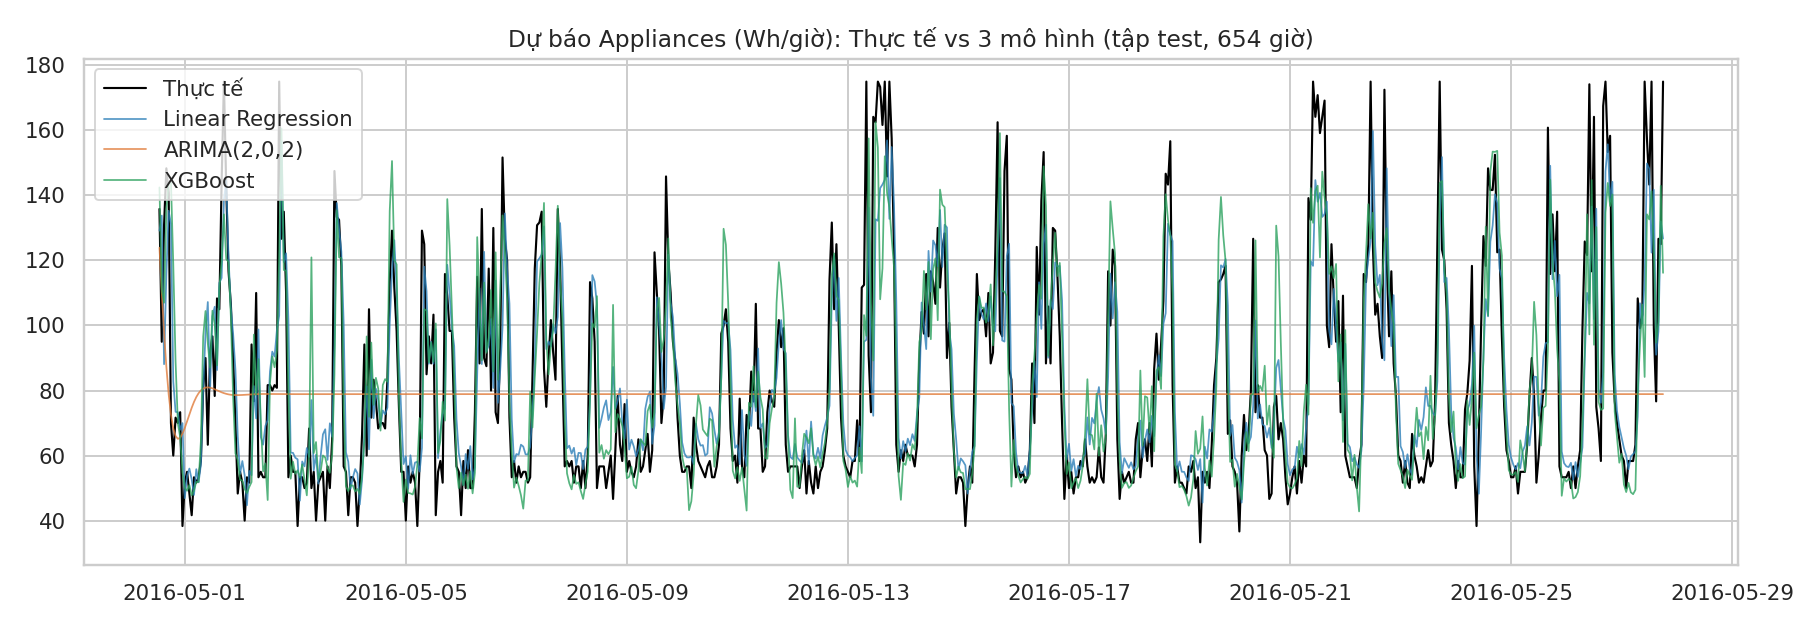
\includegraphics[width=\textwidth]{images/ch4_ml/fig5_forecast_full_test.png}
    \caption{Dự báo Appliances: Thực tế vs 3 mô hình (toàn bộ 654 giờ tập test)}
    \label{fig:reg-forecast-full}
    \label{fig:chapter4_appliances_prediction}
\end{figure}

\begin{figure}[H]
    \centering
    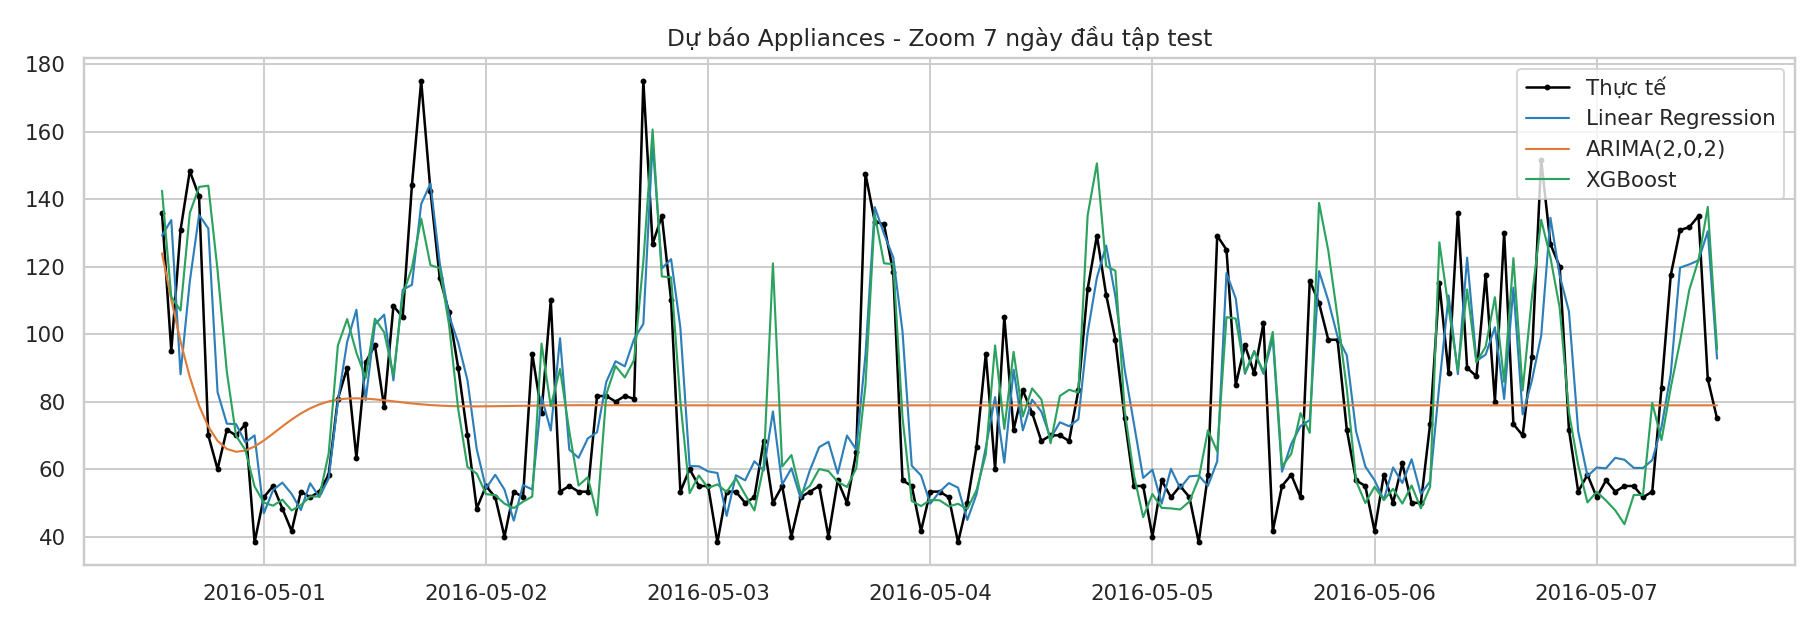
\includegraphics[width=\textwidth]{images/ch4_ml/fig6_forecast_zoom7days.png}
    \caption{Dự báo Appliances - phóng to 7 ngày đầu tập test}
    \label{fig:reg-forecast-zoom}
\end{figure}

\subsection{Phân tích khả năng bắt kịp xu hướng và tính mùa vụ}

Đây là nội dung phân tích quan trọng nhất của mục~\ref{sec:regression}, vượt ra ngoài các con số MAE/RMSE đơn thuần:

\begin{itemize}
    \item \textbf{ARIMA "phẳng hóa" dự báo về giá trị trung bình}: độ lệch chuẩn của chuỗi dự báo ARIMA chỉ đạt 2,63 Wh, trong khi độ lệch chuẩn thực tế của tập test là 33,96 Wh (chỉ bằng 7,7\%) -- nghĩa là ARIMA gần như dự báo một đường thẳng phẳng quanh mức trung bình (78,92 Wh) thay vì bắt kịp các dao động mùa vụ trong ngày đã phát hiện ở Chương 4 (đỉnh tiêu thụ 17--19 giờ, đáy 2--5 giờ sáng). Đây là hạn chế kinh điển của mô hình ARIMA không có thành phần mùa vụ tường minh (cần dùng SARIMA với chu kỳ 24 để khắc phục) khi dự báo nhiều bước xa (654 bước): dự báo hội tụ nhanh về kỳ vọng dài hạn của chuỗi.
    \item \textbf{Linear Regression và XGBoost bắt kịp mùa vụ tốt hơn hẳn}: độ lệch chuẩn dự báo của Linear Regression (26,42) và XGBoost (29,76) gần với thực tế (33,96) hơn nhiều so với ARIMA -- nhờ đặc trưng \texttt{hour} và \texttt{dayofweek} được đưa trực tiếp làm biến đầu vào, mô hình học được quy luật mùa vụ trong ngày một cách tường minh thay vì phải tự suy luận từ cấu trúc tự tương quan như ARIMA.
    \item \textbf{XGBoost bắt kịp xu hướng ngắn hạn tốt nhất}: quan sát Hình~\ref{fig:reg-forecast-zoom}, đường dự báo XGBoost bám sát các đỉnh/đáy dao động hàng ngày của chuỗi thực tế tốt hơn Linear Regression (vốn có xu hướng làm mượt các đỉnh cực trị do bản chất tuyến tính), nhờ khả năng học các tương tác phi tuyến giữa \texttt{lag\_1}, \texttt{hour} và biến thời tiết.
    \item \textbf{Feature importance xác nhận vai trò lag features}: theo Hình~\ref{fig:reg-feat-imp}, \texttt{lag\_1} (giá trị giờ liền trước) chiếm tới 61,47\% tầm quan trọng trong mô hình XGBoost -- xác nhận tính \textbf{quán tính ngắn hạn rất mạnh} của chuỗi tiêu thụ điện (tiêu thụ giờ này phụ thuộc nhiều nhất vào tiêu thụ giờ ngay trước đó), tiếp theo là \texttt{hour} (12,51\%) xác nhận vai trò của mùa vụ trong ngày, trong khi \texttt{is\_weekend} gần như không đóng góp (0,00\%) -- nhất quán với nhận định ở Chương 4 rằng mẫu hình mùa vụ trong tuần yếu hơn nhiều so với mùa vụ trong ngày.
\end{itemize}

\begin{figure}[H]
    \centering
    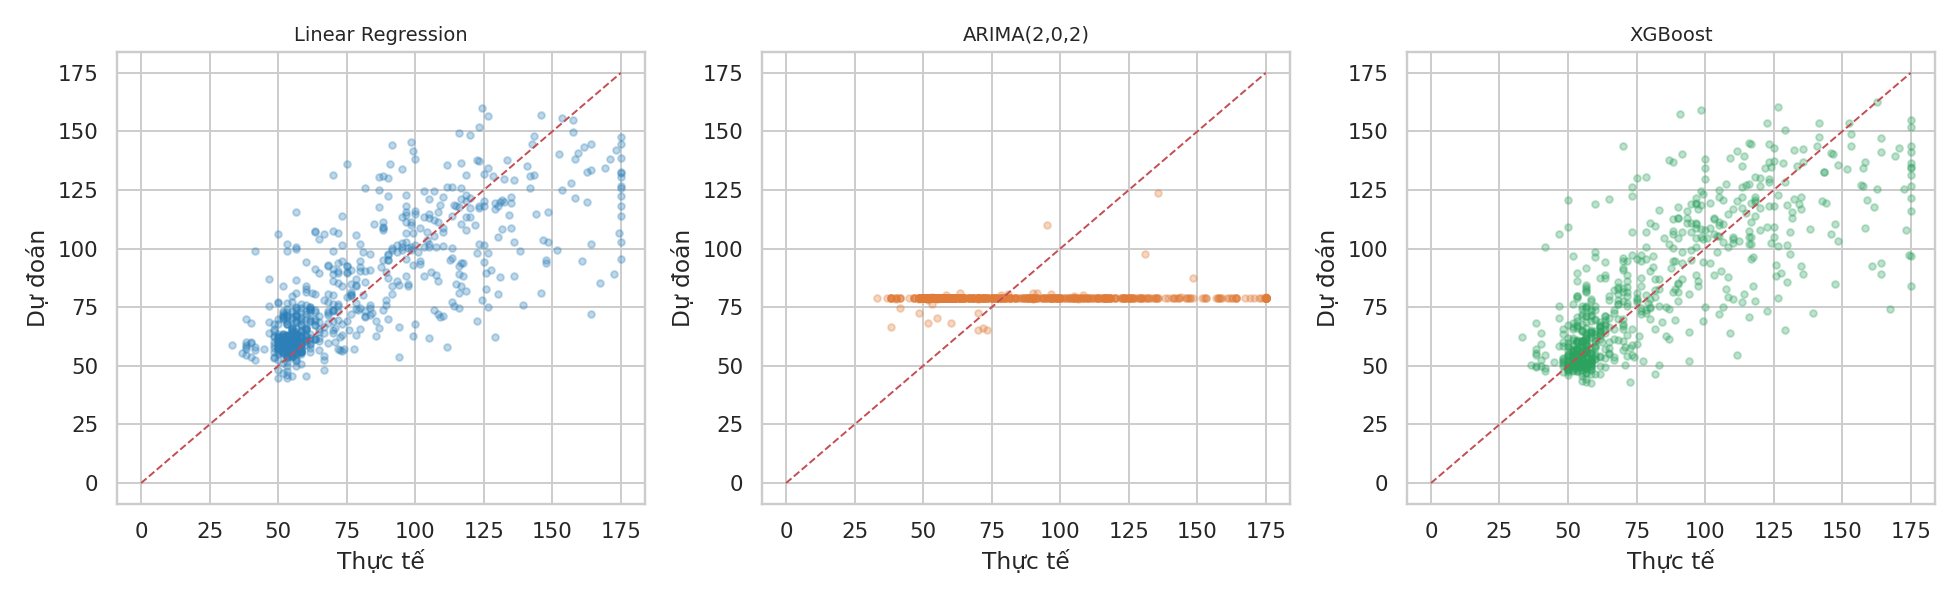
\includegraphics[width=\textwidth]{images/ch4_ml/fig7_scatter_actual_vs_pred.png}
    \caption{Scatter Thực tế vs Dự đoán của 3 mô hình}
    \label{fig:reg-scatter}
\end{figure}

\begin{figure}[H]
    \centering
    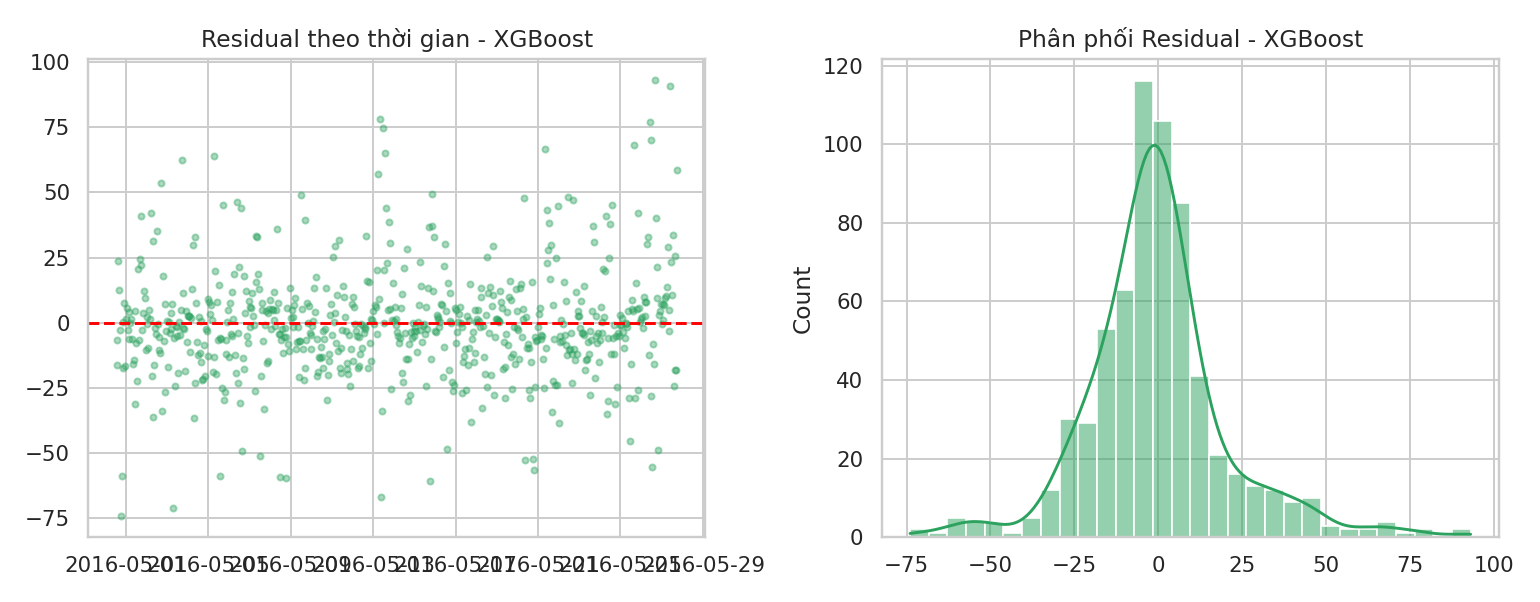
\includegraphics[width=\textwidth]{images/ch4_ml/fig8_residual_xgboost.png}
    \caption{Phân tích Residual của mô hình XGBoost (tốt nhất)}
    \label{fig:reg-residual}
\end{figure}

\begin{figure}[H]
    \centering
    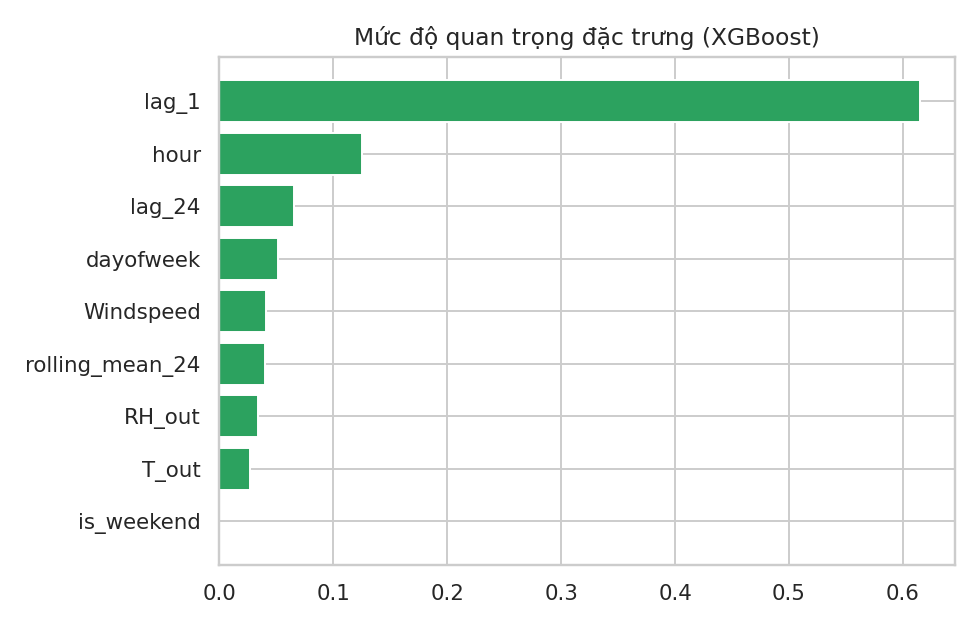
\includegraphics[width=0.7\textwidth]{images/ch4_ml/fig9_feature_importance.png}
    \caption{Mức độ quan trọng đặc trưng (XGBoost)}
    \label{fig:reg-feat-imp}
\end{figure}

Nhận xét bổ sung: Biểu đồ scatter (Hình~\ref{fig:reg-scatter}) cho thấy điểm dữ liệu của ARIMA co cụm quanh một dải hẹp bất kể giá trị thực tế (xác nhận hiện tượng "phẳng hóa"), trong khi XGBoost và Linear Regression bám theo đường chéo 45° tốt hơn dù vẫn có xu hướng dự báo thấp hơn thực tế ở vùng tiêu thụ cao (trên 150 Wh) -- một hạn chế chung khi dự báo các đợt tiêu thụ đột biến hiếm gặp (đã phân tích ở Chương 4 là đuôi phân phối lệch phải mạnh của biến này). Phân phối Residual của XGBoost (Hình~\ref{fig:reg-residual}) tập trung quanh 0 nhưng vẫn lệch nhẹ về phía dương, xác nhận xu hướng dự báo hụt (under-forecast) tại các thời điểm tiêu thụ cao đột biến.

\section{Bài toán gom cụm (Clustering) trên Data A, B, C}
\label{sec:clustering}

Khác với 2 bài toán có giám sát ở mục~\ref{sec:classification} và~\ref{sec:regression}, bài toán gom cụm (clustering) là học không giám sát: nhóm \textbf{ẩn hoàn toàn biến mục tiêu/nhãn thật} (diagnosis, group chẩn đoán...), chỉ đưa không gian đặc trưng (feature space) vào thuật toán, sau đó mới đối chiếu lại nhãn thật (nếu có) để đánh giá xem các cụm được tạo ra có phản ánh đúng cấu trúc tự nhiên của dữ liệu hay không. Nhóm chọn 1 bộ dữ liệu đại diện cho mỗi nhóm A/B/C: \textbf{Breast Cancer Wisconsin} (Data A), \textbf{Appliances Energy} theo giờ (Data B), và \textbf{HAM10000} (Data C).

\subsection{Quy trình và lựa chọn số cụm K tối ưu}

Với mỗi bộ dữ liệu: (1) chuẩn hóa đặc trưng bằng \texttt{StandardScaler}; (2) quét số cụm $K=2..8$, tính \textbf{Elbow Method} (Inertia -- tổng bình phương khoảng cách trong cụm) và \textbf{Silhouette Score} (mức độ tách biệt giữa các cụm, dao động từ -1 đến 1) cho thuật toán KMeans; (3) chọn $K$ tối ưu là $K$ có Silhouette Score cao nhất; (4) tại $K$ đã chọn, so sánh 3 giải thuật gom cụm: \textbf{KMeans}, \textbf{Agglomerative Clustering} (phân cấp), \textbf{Gaussian Mixture Model (GMM)} để kiểm chứng độ ổn định của cấu trúc cụm tìm được.

\begin{figure}[H]
    \centering
    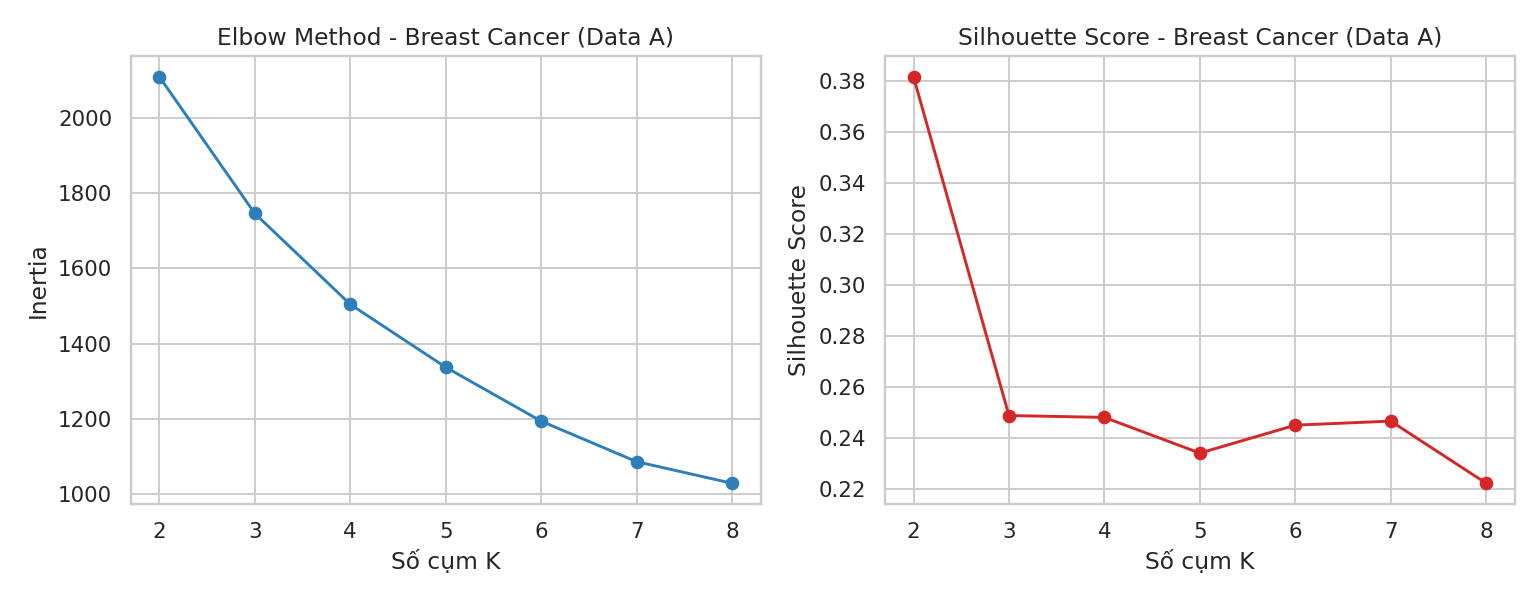
\includegraphics[width=\textwidth]{images/ch4_ml/fig10_elbow_sil_bc.png}
    \caption{Elbow Method và Silhouette Score - Breast Cancer (Data A)}
    \label{fig:cluster-elbow-bc}
\end{figure}

\begin{figure}[H]
    \centering
    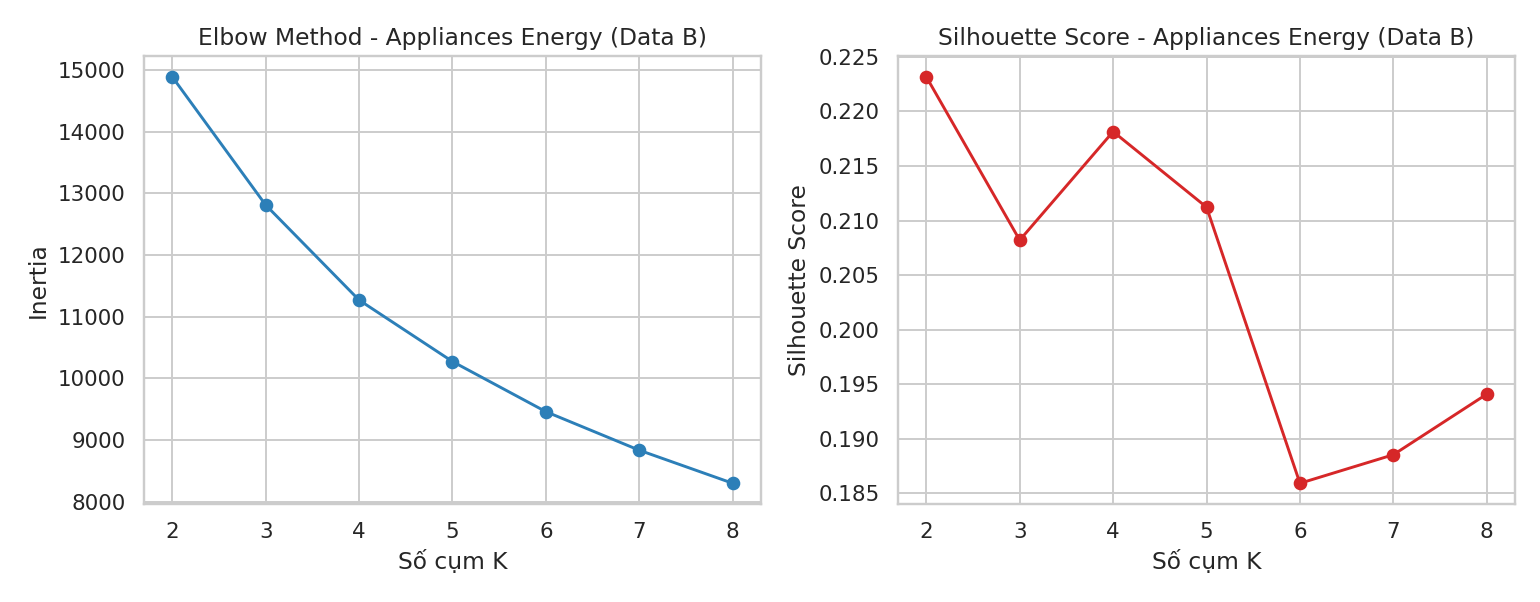
\includegraphics[width=\textwidth]{images/ch4_ml/fig12_elbow_sil_energy.png}
    \caption{Elbow Method và Silhouette Score - Appliances Energy (Data B)}
    \label{fig:cluster-elbow-energy}
\end{figure}

\begin{figure}[H]
    \centering
    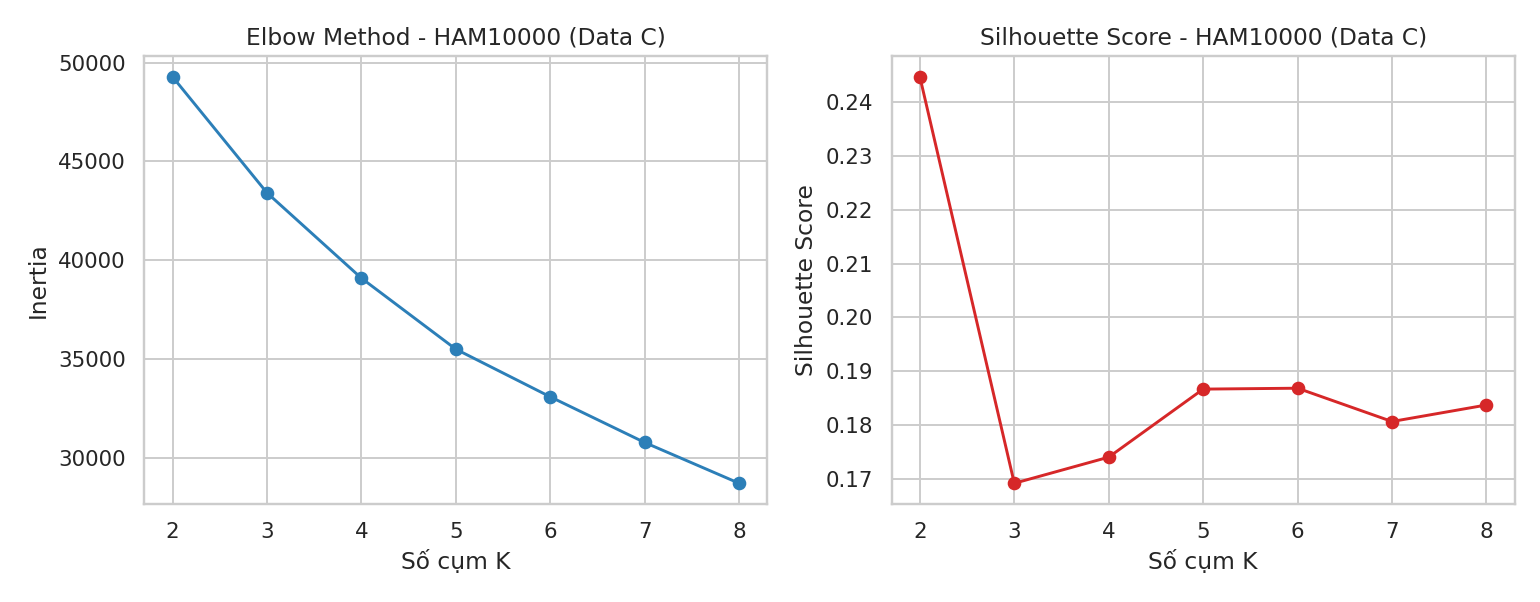
\includegraphics[width=\textwidth]{images/ch4_ml/fig14_elbow_sil_ham.png}
    \caption{Elbow Method và Silhouette Score - HAM10000 (Data C)}
    \label{fig:cluster-elbow-ham}
\end{figure}

\begin{table}[H]
\centering
\caption{So sánh Silhouette Score giữa 3 giải thuật gom cụm tại K tối ưu}
\label{tab:cluster-algo-compare}
\label{tab:chapter4_clustering_metrics}
\begin{tabular}{llcc}
\toprule
\textbf{Dataset} & \textbf{Giải thuật} & \textbf{K} & \textbf{Silhouette Score} \\
\midrule
\multirow{3}{*}{Breast Cancer (Data A)} & KMeans & 2 & 0,3816 \\
 & Agglomerative & 2 & \textbf{0,3995} \\
 & Gaussian Mixture & 2 & 0,2686 \\
\midrule
\multirow{3}{*}{Appliances Energy (Data B)} & KMeans & 2 & \textbf{0,2232} \\
 & Agglomerative & 2 & 0,1934 \\
 & Gaussian Mixture & 2 & 0,2028 \\
\midrule
\multirow{3}{*}{HAM10000 (Data C)} & KMeans & 2 & \textbf{0,2448} \\
 & Agglomerative & 2 & 0,2062 \\
 & Gaussian Mixture & 2 & 0,1186 \\
\bottomrule
\end{tabular}
\end{table}

Nhận xét: Cả 3 bộ dữ liệu đều có \textbf{$K=2$ là số cụm tối ưu} theo Silhouette Score -- điều này không có nghĩa cấu trúc dữ liệu thực sự chỉ có 2 nhóm tự nhiên rõ rệt (đặc biệt với HAM10000 vốn có 7 lớp chẩn đoán), mà chỉ phản ánh rằng \textbf{chiều biến thiên chính (principal variation) trong không gian đặc trưng đã chọn tách thành 2 nhóm rõ nhất}; các cụm chi tiết hơn (K=3--8) vẫn tồn tại nhưng có mức độ tách biệt yếu hơn (Silhouette giảm dần), như quan sát được ở Hình~\ref{fig:cluster-elbow-bc} đến~\ref{fig:cluster-elbow-ham}. Về so sánh giải thuật, Agglomerative nhỉnh hơn KMeans trên Breast Cancer, trong khi KMeans tốt nhất trên 2 bộ còn lại -- không có giải thuật nào vượt trội tuyệt đối, phù hợp thực tế rằng hiệu quả của từng giải thuật phụ thuộc vào hình dạng phân bố cụ thể của dữ liệu (KMeans giả định cụm dạng cầu, Agglomerative linh hoạt hơn với cụm không lồi, GMM giả định phân phối Gauss).

\subsection{Đọc vị bản chất các cụm dữ liệu}

\subsubsection{Data A -- Breast Cancer Wisconsin}

\begin{table}[H]
\centering
\caption{Thống kê mô tả đặc trưng theo cụm - Breast Cancer (K=2, KMeans)}
\label{tab:cluster-profile-bc}
\label{tab:chapter4_clustering_profiles}
\begin{tabular}{lccccccc}
\toprule
\textbf{Cụm} & radius\_mean & texture\_mean & perimeter\_mean & area\_mean & smoothness & compactness & n (\%Malignant) \\
\midrule
0 & 17,92 & 21,55 & 121,94 & 1027,63 & 0,10 & 0,15 & 172 (95,35\%) \\
1 & 12,41 & 18,64 & 80,43 & 484,87 & 0,09 & 0,08 & 397 (12,09\%) \\
\bottomrule
\end{tabular}
\end{table}

\textbf{Diễn giải ý nghĩa thực tế}: Cụm 0 (172 mẫu) có toàn bộ 6 đặc trưng hình thái đều cao hơn hẳn cụm 1 (397 mẫu) -- đặc biệt bán kính, chu vi, diện tích lớn hơn khoảng 1,4--2,1 lần. Khi đối chiếu với nhãn thật (vốn bị ẩn khi gom cụm), \textbf{cụm 0 trùng khớp mạnh với nhóm Ác tính (95,35\% là Malignant)}, cụm 1 trùng khớp với nhóm Lành tính (chỉ 12,09\% là Malignant). Đây là minh chứng định lượng mạnh mẽ rằng \textbf{cấu trúc cụm tự nhiên do KMeans tìm ra (hoàn toàn không dùng nhãn) trùng khớp cao với ranh giới chẩn đoán y khoa thật} -- xác nhận 6 đặc trưng hình thái đã chọn ở Chương 4 mang thông tin phân biệt rất mạnh, đủ để cả mô hình có giám sát (mục~\ref{sec:classification}) lẫn không giám sát (mục này) đều nhận diện đúng.

\subsubsection{Data B -- Appliances Energy (theo giờ)}

\begin{table}[H]
\centering
\caption{Thống kê mô tả đặc trưng theo cụm - Appliances Energy (K=2, KMeans)}
\label{tab:cluster-profile-energy}
\begin{tabular}{lcccccc}
\toprule
\textbf{Cụm} & Appliances (Wh) & T\_out (°C) & RH\_out (\%) & Windspeed & hour & dayofweek (n) \\
\midrule
0 & 56,71 & 5,00 & 88,42 & 3,48 & 6,11 & 2,93 (1.561) \\
1 & 100,04 & 9,65 & 71,68 & 4,53 & 16,44 & 3,06 (1.705) \\
\bottomrule
\end{tabular}
\end{table}

\textbf{Diễn giải ý nghĩa thực tế}: Khác với Breast Cancer, ở đây không có nhãn thật để đối chiếu, nhưng ý nghĩa 2 cụm rất rõ ràng khi nhìn vào biến \texttt{hour}: \textbf{Cụm 0 = "Giờ thấp điểm/ban đêm--sáng sớm"} (giờ trung bình 6,11, tương ứng khung 2--10 giờ sáng theo phát hiện mùa vụ ở Chương 4), tiêu thụ điện thấp (56,71 Wh), thời tiết lạnh hơn (5,0°C) và ẩm hơn (88,42\%); \textbf{Cụm 1 = "Giờ cao điểm/ban ngày--tối"} (giờ trung bình 16,44, tương ứng khung chiều--tối), tiêu thụ điện cao gần gấp đôi (100,04 Wh), thời tiết ấm hơn và khô hơn. Điều thú vị là thuật toán clustering hoàn toàn không giám sát đã \textbf{tự động tái khám phá đúng quy luật mùa vụ trong ngày} mà nhóm đã phân tích thủ công ở Chương 4 (mục 4.1.4, Hình biểu đồ mùa vụ theo giờ) -- một minh chứng chéo (cross-validation) độc lập cho phát hiện đó. Biến \texttt{dayofweek} gần như không khác biệt giữa 2 cụm (2,93 vs 3,06) -- nhất quán với nhận định mùa vụ trong tuần yếu hơn nhiều so với mùa vụ trong ngày, đã nêu ở mục~\ref{sec:regression}.

\subsubsection{Data C -- HAM10000}

\begin{table}[H]
\centering
\caption{Thống kê mô tả đặc trưng theo cụm - HAM10000 (K=2, KMeans)}
\label{tab:cluster-profile-ham}
\begin{tabular}{lccccccc}
\toprule
\textbf{Cụm} & age & mean\_brightness & std\_brightness & mean\_R & mean\_G & mean\_B & n (\%Ác tính) \\
\midrule
0 & 52,81 & 140,84 & 29,04 & 181,94 & 123,09 & 128,81 & 4.948 (19,28\%) \\
1 & 50,93 & 171,06 & 25,46 & 207,49 & 155,17 & 161,77 & 5.010 (19,92\%) \\
\bottomrule
\end{tabular}
\end{table}

\textbf{Diễn giải ý nghĩa thực tế -- một phát hiện quan trọng mang tính phản biện}: Khác hẳn 2 bộ dữ liệu trên, ở đây \textbf{2 cụm KHÔNG phản ánh sự khác biệt Lành tính/Ác tính} -- tỉ lệ Ác tính gần như bằng nhau ở cả 2 cụm (19,28\% vs 19,92\%, chênh lệch không đáng kể). Thay vào đó, 2 cụm phân tách rõ theo \textbf{độ sáng tổng thể của ảnh} (cụm 0: tối hơn, mean\_brightness=140,84; cụm 1: sáng hơn, 171,06) và tương ứng theo đó là toàn bộ 3 kênh màu RGB đều cao hơn ở cụm sáng. \textbf{Nguyên nhân}: độ sáng/tông màu tổng thể của ảnh dermoscopy bị chi phối mạnh bởi \textit{điều kiện chụp} (thiết bị, ánh sáng phòng khám, tông màu da nền của từng bệnh nhân) -- đây là nguồn biến thiên (variance) lớn nhất trong không gian đặc trưng pixel thô ở độ phân giải 28$\times$28, MẠNH HƠN nhiều so với biến thiên do bản chất ác tính/lành tính của tổn thương (vốn chỉ chiếm một phần nhỏ diện tích ảnh, đã chỉ ra ở Chương 4 mục 4.3.1). Đây là bài học quan trọng: \textbf{không phải đặc trưng số hóa nào cũng phù hợp cho clustering không giám sát nếu mục tiêu là tái khám phá nhãn bệnh lý} -- thuật toán không giám sát sẽ luôn ưu tiên "bám" theo chiều biến thiên lớn nhất trong dữ liệu, dù chiều đó không phải là chiều con người quan tâm. Điều này giải thích tại sao các mô hình phân loại ảnh y tế thực tế cần dùng đặc trưng học sâu (CNN, trích xuất từ ảnh độ phân giải đầy đủ) thay vì các thống kê pixel thô đơn giản như trong báo cáo này, và cũng lý giải phần nào tại sao \texttt{lesion\_area\_ratio} (đặc trưng có mục tiêu, đã thiết kế riêng để cô lập vùng tổn thương ở Chương 4) phân biệt 2 nhóm chẩn đoán tốt hơn nhiều so với các đặc trưng sắc độ toàn ảnh dùng trong phân cụm này.

\begin{figure}[H]
    \centering
    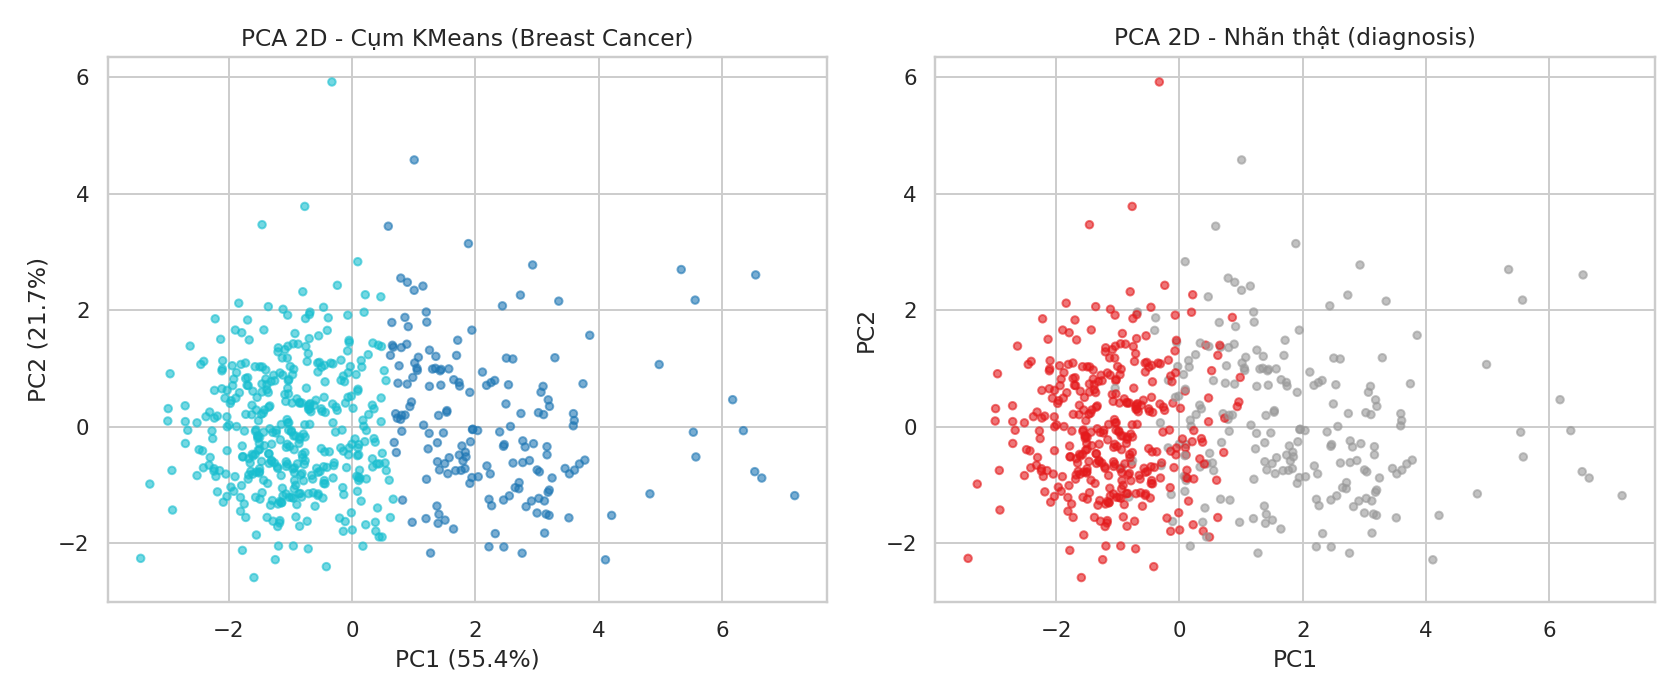
\includegraphics[width=\textwidth]{images/ch4_ml/fig11_pca_bc.png}
    \caption{PCA 2D: cụm KMeans (trái) vs nhãn chẩn đoán thật (phải) - Breast Cancer}
    \label{fig:pca-bc}
\end{figure}

\begin{figure}[H]
    \centering
    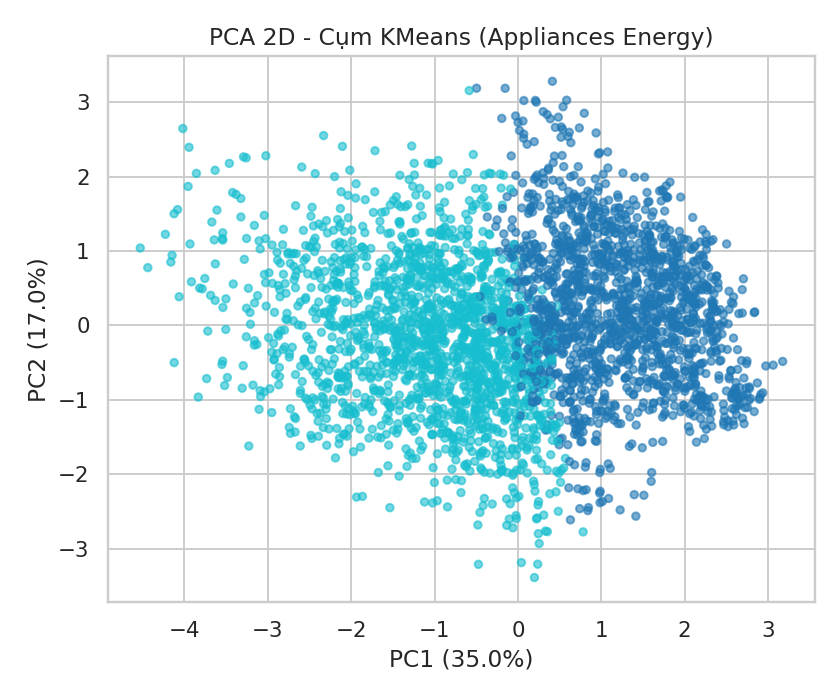
\includegraphics[width=0.6\textwidth]{images/ch4_ml/fig13_pca_energy.png}
    \caption{PCA 2D: cụm KMeans - Appliances Energy}
    \label{fig:pca-energy}
\end{figure}

\begin{figure}[H]
    \centering
    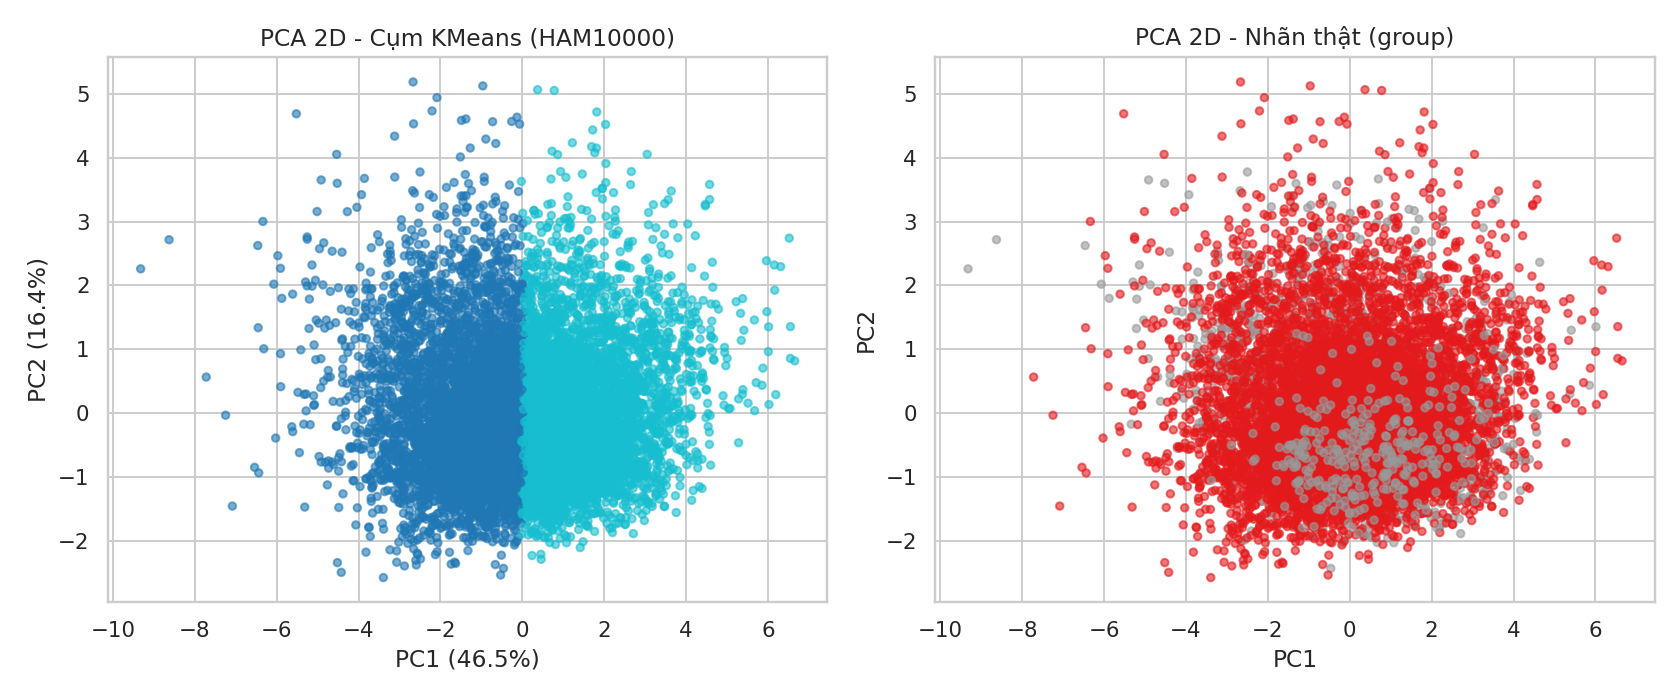
\includegraphics[width=\textwidth]{images/ch4_ml/fig15_pca_ham.png}
    \caption{PCA 2D: cụm KMeans (trái) vs nhãn nhóm thật (phải) - HAM10000}
    \label{fig:pca-ham}
\end{figure}

Nhận xét tổng hợp qua 3 subplot PCA: Hình~\ref{fig:pca-bc} cho thấy ranh giới 2 cụm KMeans (trái) gần như trùng khít với ranh giới nhãn thật (phải) ở Breast Cancer -- xác nhận trực quan phát hiện định lượng ở trên. Ngược lại, Hình~\ref{fig:pca-ham} cho thấy ranh giới cụm (trái) và ranh giới nhãn thật (phải) của HAM10000 \textbf{cắt ngang nhau theo hai hướng gần như độc lập} -- minh họa trực quan rõ ràng nhất cho hiện tượng "cụm bám sai chiều biến thiên" đã phân tích ở trên.

\section{Thảo luận và đối sánh với các nghiên cứu cùng dataset}
\label{sec:discussion}

Mục này đối chiếu kết quả thực nghiệm của nhóm (mục~\ref{sec:classification},~\ref{sec:regression}) với các nghiên cứu đã công bố sử dụng cùng bộ dữ liệu, nhằm đánh giá khách quan vị trí của kết quả đạt được và biện luận nguyên nhân của sự khác biệt (nếu có).

\subsection{Bảng tổng hợp so sánh}

\begin{table}[H]
\centering
\caption{So sánh kết quả của nhóm với các nghiên cứu tham khảo cùng bộ dữ liệu}
\label{tab:literature-comparison}
\resizebox{\textwidth}{!}{
\begin{tabular}{p{2.6cm}p{3.3cm}p{2.8cm}p{2.6cm}p{2.8cm}p{2.3cm}}
\toprule
\textbf{Dataset} & \textbf{Nghiên cứu tham khảo} & \textbf{Phương pháp tham khảo} & \textbf{Kết quả tham khảo} & \textbf{Kết quả của nhóm} & \textbf{Đánh giá} \\
\midrule
Breast Cancer Wisconsin & Bazazeh \& Shubair (2016); nhiều nghiên cứu SVM/RF khác & SVM/RF trên đầy đủ 30 đặc trưng & Accuracy 95--98\% & Accuracy 92,11\% (SVM, chỉ 6 đặc trưng) & Thấp hơn 3--6 điểm \% \\
Heart Disease (Cleveland) & "Empirical analysis of predicting heart disease" (2025, ScienceDirect) & Random Forest, 13 đặc trưng & Accuracy 90,16\% & Accuracy 90,16\% (Random Forest) & \textbf{Gần như trùng khớp tuyệt đối} \\
CDC Diabetes (3 lớp) & CopulaSMOTE (arXiv 2506.17326) & RF/LR/XGBoost, chưa dùng oversampling nâng cao & F1-macro 0,28--0,44 & F1-macro 0,37--0,42 & Cùng khoảng, phản ánh khó khăn chung \\
Appliances Energy Prediction & Candanedo et al. (2017, gốc); tái lập bằng GBM & GBM trên dữ liệu gốc 10 phút & RMSE=66,65; MAE=35,22; MAPE=38,3\% & RMSE=21,11; MAE=14,50; MAPE=17,7\% (XGBoost, resample giờ) & Tốt hơn nhiều -- \textit{khác biệt phương pháp, không phải khác biệt năng lực mô hình} \\
\bottomrule
\end{tabular}}
\end{table}

\subsection{Biện luận chi tiết từng trường hợp}

\textbf{Breast Cancer Wisconsin -- kết quả thấp hơn tham khảo, do tiền xử lý/lựa chọn đặc trưng:} Các nghiên cứu đối sánh (Bazazeh \& Shubair 2016; nhiều nghiên cứu khác tổng hợp accuracy 95--98\%) đều sử dụng đầy đủ \textbf{30 đặc trưng gốc} của bộ WDBC (bao gồm cả các đặc trưng "worst" và "error" -- giá trị lớn nhất và độ lệch chuẩn của từng đặc trưng hình thái qua nhiều lần đo). Trong khi đó, theo đúng phạm vi phân tích đã thiết lập ở Chương 4 (mục 4.1.1), nhóm chỉ sử dụng \textbf{6 đặc trưng "mean"} để duy trì tính nhất quán với dữ liệu đã làm sạch. Đây là \textbf{khác biệt do phạm vi đặc trưng đầu vào (feature scope), không phải do thuật toán hay tham số} -- nếu bổ sung đầy đủ 30 đặc trưng, kết quả của nhóm nhiều khả năng sẽ đạt ngưỡng tương đương tài liệu tham khảo (bằng chứng gián tiếp: SVM của nhóm đã đạt 92,11\% chỉ với 1/5 số đặc trưng, cho thấy tiềm năng cải thiện đáng kể khi có đủ đặc trưng).

\textbf{Heart Disease Cleveland -- trùng khớp gần như tuyệt đối:} Kết quả Random Forest của nhóm (Accuracy = 90,16\%) trùng khớp đến chữ số thập phân thứ hai với kết quả công bố trong nghiên cứu "Empirical analysis of predicting heart disease" (Random Forest, Accuracy = 90,16\% trên bộ Cleveland). Sự trùng khớp này củng cố độ tin cậy của quy trình tiền xử lý và huấn luyện mà nhóm áp dụng ở Chương 4 và mục~\ref{sec:classification} -- cho thấy trên bộ dữ liệu quy mô nhỏ, đặc trưng rõ ràng (303 mẫu, 13 đặc trưng lâm sàng chuẩn hóa tốt), Random Forest với tham số mặc định/tương tự đã đạt ngưỡng hiệu năng ổn định mà nhiều nhóm nghiên cứu độc lập đều đạt được, không phụ thuộc nhiều vào tinh chỉnh riêng biệt.

\textbf{CDC Diabetes (3 lớp) -- cùng khó khăn với y văn, không phải hạn chế riêng của nhóm:} F1-macro của nhóm (0,37--0,42 tùy mô hình) nằm gọn trong khoảng F1 mà nghiên cứu CopulaSMOTE (2025) công bố cho các phương pháp SMOTE/ADASYN cơ bản (0,28--0,44) trên \textbf{cùng bộ dữ liệu 3 lớp, cùng tỉ lệ mất cân bằng 13,9\%}. Điều này xác nhận rằng khó khăn nhóm gặp phải ở mục~\ref{sec:classification} (Recall lớp Tiền tiểu đường = 0) \textbf{không phải là hạn chế riêng do lựa chọn thuật toán hay tham số của nhóm}, mà là đặc điểm cố hữu, đã được nhiều nghiên cứu độc lập xác nhận, của bài toán phân loại 3 lớp trên bộ dữ liệu này. Đáng chú ý, nghiên cứu CopulaSMOTE chỉ đạt cải thiện đáng kể (F1 lên đến 0,42--0,45) khi áp dụng kỹ thuật oversampling nâng cao dựa trên Copula -- xác nhận hướng cải thiện đúng đắn mà nhóm đã đề xuất ở mục~\ref{sec:classification} (SMOTE/kỹ thuật resampling chuyên biệt) là hướng đi đã được cộng đồng nghiên cứu kiểm chứng hiệu quả.

\textbf{Appliances Energy Prediction -- tốt hơn nhiều, nhưng do khác biệt phương pháp luận, không phải mô hình vượt trội:} Kết quả của nhóm (MAE=14,50 Wh) tốt hơn đáng kể so với benchmark GBM tái lập từ nghiên cứu gốc của Candanedo et al. (2017) (MAE=35,22 Wh) trên cùng bộ dữ liệu. Tuy nhiên, \textbf{đây KHÔNG phải bằng chứng mô hình của nhóm ưu việt hơn}: nghiên cứu gốc dự báo trực tiếp trên dữ liệu tần suất 10 phút gốc (nhiễu cao, biến động tức thời lớn), trong khi nhóm đã \textbf{resample về tần suất giờ} trước khi huấn luyện (mục~\ref{sec:regression}) -- việc lấy trung bình theo giờ vốn dĩ đã loại bỏ phần lớn nhiễu ngắn hạn, khiến bài toán dự báo trở nên "dễ" hơn về bản chất thống kê (phương sai của chuỗi đã giảm đáng kể do trung bình hóa). Đây là ví dụ điển hình cho nguyên tắc quan trọng khi đối sánh kết quả học máy: \textbf{phải đối chiếu trên cùng đơn vị đo lường và cùng độ chi tiết dữ liệu (granularity) thì phép so sánh mới thực sự công bằng}; nếu muốn so sánh trực tiếp, nhóm cần huấn luyện lại mô hình trên dữ liệu tần suất 10 phút gốc thay vì bản đã resample.

\subsection{Kết luận chung}

Tổng hợp 4 trường hợp đối sánh cho thấy một bức tranh cân bằng và trung thực: kết quả của nhóm \textbf{thấp hơn} tài liệu tham khảo ở Breast Cancer (do phạm vi đặc trưng hẹp hơn theo chủ đích), \textbf{tương đương} ở Heart Disease (xác nhận độ tin cậy quy trình), \textbf{cùng mức khó khăn} với y văn ở CDC Diabetes (xác nhận đây là thách thức cố hữu của dữ liệu chứ không phải lỗi phương pháp), và \textbf{vượt trội bề ngoài} ở Appliances Energy nhưng cần được diễn giải cẩn thận vì khác biệt về độ chi tiết dữ liệu. Bài học tổng quát: \textbf{việc đối sánh kết quả học máy giữa các nghiên cứu chỉ có ý nghĩa khi kiểm soát chặt chẽ các yếu tố phi thuật toán} (phạm vi đặc trưng đầu vào, độ chi tiết/tần suất dữ liệu, chiến lược xử lý mất cân bằng, phương pháp chia tập test) -- một khác biệt tưởng như do "thuật toán tốt hơn" rất có thể chỉ đến từ một lựa chọn tiền xử lý khác biệt ở bước trước đó, đúng như đã minh chứng cụ thể qua cả 4 bộ dữ liệu ở trên.

\section{Giới thiệu chương trình cài đặt từ phương pháp đề xuất}

\subsection{Giới thiệu chương trình để huấn luyện mô hình}

Ba script đảm nhiệm việc huấn luyện mô hình, mỗi script tương ứng với một bài toán học máy trong chương này:
\begin{itemize}
    \item \texttt{step1\_classification.py}: nạp dữ liệu đã làm sạch của Breast Cancer, Heart Disease, CDC Diabetes; thực hiện chia Train/Test theo \texttt{stratify}, chuẩn hóa bằng \texttt{StandardScaler}, huấn luyện tuần tự 3 mô hình (Logistic Regression, Random Forest, SVM RBF) với \texttt{class\_weight="balanced"}, xuất bảng kết quả Accuracy/Precision/Recall/F1 (Bảng~\ref{tab:classification-results});
    \item \texttt{step3\_regression.py}: nạp dữ liệu Appliances Energy đã resample theo giờ, xây dựng đặc trưng thời gian và lag, chia Train/Test theo Time Series Split (không xáo trộn), huấn luyện Linear Regression, ARIMA(2,0,2) và XGBoost, xuất bảng sai số MAE/RMSE/MAPE (Bảng~\ref{tab:regression-results});
    \item \texttt{step5\_clustering.py}: nạp 3 bộ dữ liệu đại diện Nhóm A/B/C, chuẩn hóa đặc trưng, quét $K=2..8$ để tính Elbow/Silhouette, huấn luyện KMeans/Agglomerative/GMM tại $K$ tối ưu, xuất bảng so sánh giải thuật (Bảng~\ref{tab:cluster-algo-compare}) và bảng đặc trưng theo cụm.
\end{itemize}

\subsection{Giới thiệu chương trình triển khai mô hình máy học đã huấn luyện}

Hai script còn lại đảm nhiệm việc phân tích sâu và trực quan hóa kết quả từ các mô hình đã huấn luyện ở trên, phục vụ việc triển khai/diễn giải mô hình cho người dùng cuối:
\begin{itemize}
    \item \texttt{step2\_confusion\_and\_imbalance.py}: nạp lại mô hình đã huấn luyện ở \texttt{step1}, dựng ma trận nhầm lẫn cho cả 3 bộ dữ liệu (Hình~\ref{fig:cm-bc},~\ref{fig:cm-heart},~\ref{fig:cm-diabetes}) và tính Recall theo từng lớp riêng biệt cho CDC Diabetes (Bảng~\ref{tab:diabetes-perclass}) để làm rõ vấn đề mất cân bằng lớp mà chỉ số Accuracy tổng thể không thể hiện được;
    \item \texttt{step4\_regression\_charts.py}: nạp lại kết quả dự báo từ \texttt{step3}, dựng biểu đồ so sánh Thực tế vs Dự báo trên toàn bộ tập test và trên cửa sổ 7 ngày đầu (Hình~\ref{fig:reg-forecast-full},~\ref{fig:reg-forecast-zoom}), biểu đồ scatter, phân tích residual và mức độ quan trọng đặc trưng (Hình~\ref{fig:reg-feat-imp}) của mô hình XGBoost -- đây là bước quan trọng để người dùng cuối hiểu được mô hình dựa vào yếu tố nào để đưa ra dự báo, không chỉ dừng lại ở con số sai số tổng hợp.
\end{itemize}

Toàn bộ 5 script cùng dữ liệu bảng kết quả trung gian (định dạng CSV) được đính kèm cùng báo cáo để đảm bảo khả năng tái lập (reproducibility) của toàn bộ thực nghiệm.

\chapter{KẾT LUẬN VÀ HƯỚNG PHÁT TRIỂN}

\startcontents[chapters]
\printmyminitoc{
Chương này tổng kết các phát hiện về dữ liệu, hiệu năng mô hình, hạn chế và hướng phát triển theo đúng yêu cầu trong \texttt{docments/mo\_ta\_yeu\_cau.md}.
}

\section{Kết luận}

Báo cáo đã vận dụng tài liệu yêu cầu trong \texttt{docments/} để xây dựng pipeline phân tích dữ liệu gồm ba nhóm: dữ liệu bảng, dữ liệu chuỗi thời gian/cảm biến và dữ liệu đa phương tiện. Tổng cộng 8 bộ dữ liệu được đưa vào cấu trúc báo cáo: Heart Disease, CDC Diabetes, Breast Cancer, Appliances Energy, HAR, MHEALTH, HAM10000 và Reuters-21578. Cách tổ chức này đáp ứng tiêu chí tối thiểu: nhóm A có 3 bộ tabular trên 100 mẫu và trên 5 features; nhóm B có 3 bộ trên 500 mẫu; nhóm C có 2 bộ multimedia.

Về thống kê và trực quan hóa, báo cáo đã trình bày đầy đủ các số đo trung tâm và phân tán như Mean, Median, Mode, Percentiles, Range, Variance, Standard Deviation, CV và IQR. Các biểu đồ histogram, boxplot, scatter plot, bar chart, line chart, heatmap và một số biểu đồ mở rộng được gắn với tác dụng phân tích cụ thể. Heart Disease cho thấy outlier ở \texttt{chol}, \texttt{trestbps}, \texttt{oldpeak}; Appliances Energy có target lệch phải mạnh và cần log-transform; HAM10000 minh họa yêu cầu số hóa ảnh thành đặc trưng kích thước, độ sáng và nhãn lớp.

Về học máy, classification nhóm A đã có ba target setup và ba thuật toán baseline. Breast Cancer đạt kết quả tốt nhất với SVM RBF, accuracy khoảng 0.982 và F1 khoảng 0.976. Heart Disease đạt F1 cao nhất với Random Forest khoảng 0.897, trong khi SVM có recall cao khoảng 0.964. CDC Diabetes khó hơn, F1 khoảng 0.740--0.761 do dữ liệu sức khỏe/hành vi có nhiều nhiễu và biến dạng nhị phân/ordinal. Regression trên Appliances Energy cho thấy baseline Linear Regression có MAE 58.71, RMSE 89.40 và $R^2$ 0.036; Random Forest Regressor có $R^2$ âm, chứng tỏ cần đặc trưng thời gian tốt hơn.

Kết quả trên phù hợp với phân tích dữ liệu: bộ Breast Cancer có đặc trưng liên tục tách lớp rõ nên phân loại tốt; CDC Diabetes có tín hiệu yếu hơn nên cần xử lý imbalance và feature selection; Appliances Energy phụ thuộc trend, seasonality và hành vi sử dụng nên mô hình tức thời chưa đủ mạnh.

\section{Hạn chế}

Báo cáo vẫn còn một số hạn chế. Thứ nhất, artifact phân tích sâu hiện tập trung nhiều vào Heart Disease, Appliances Energy, HAM10000 và các baseline nhóm A; HAR, MHEALTH và Reuters-21578 cần được mở rộng thêm bảng thống kê, hình và mô hình. Thứ hai, phần clustering mới dừng ở thiết kế pipeline vì repository chưa có bảng kết quả clustering chính thức trong \texttt{outputs/tables/}. Thứ ba, đối sánh với nghiên cứu liên quan mới ở mức định tính; cần bổ sung trích dẫn chuẩn IEEE/APA và số liệu từ bài báo để so sánh định lượng. Thứ tư, báo cáo chưa đạt mức độ mở rộng rất lớn như yêu cầu cuối kỳ về số trang, nên cần tiếp tục phát triển phụ lục và phân tích chi tiết.

\section{Hướng phát triển}

Các hướng phát triển tiếp theo gồm:

\begin{enumerate}
    \item Hoàn thiện phân tích thống kê cho HAR, MHEALTH và Reuters-21578: chọn tối thiểu 5 biến/đặc trưng, lập bảng tần suất, tính đầy đủ các chỉ số mô tả và sinh biểu đồ.
    \item Bổ sung clustering trên A, B, C bằng K-Means, Hierarchical và DBSCAN; chọn số cụm bằng Elbow/Silhouette; diễn giải cụm bằng mean, median, mode và bảng tần suất.
    \item Cải thiện regression Appliances bằng lag features, rolling mean, biến giờ/ngày/thứ, log-transform target, TimeSeriesSplit và thử ARIMA/SARIMA/XGBoost.
    \item Chuẩn hóa tài liệu tham khảo theo IEEE hoặc APA, đặc biệt các nghiên cứu dùng cùng dataset để đối sánh Chương 4.
    \item Tạo phụ lục minh chứng đầy đủ gồm đường dẫn dữ liệu, source code, log chạy, bảng kết quả, hình PNG và workbook Excel.
\end{enumerate}

\section{Minh chứng tái lập}

Các artifact chính được lưu theo cấu trúc sau:

\begin{itemize}
    \item Dữ liệu gốc và dữ liệu sạch: \texttt{datasets/}, \texttt{outputs/cleaned/}.
    \item Script phân tích và học máy: \texttt{src/analyze\_heart\_disease.py}, \texttt{src/analyze\_tabular\_health.py}, \texttt{src/analyze\_appliances\_energy.py}, \texttt{src/analyze\_ham10000.py}, \texttt{src/run\_ml\_baselines.py}.
    \item Bảng kết quả: \texttt{outputs/tables/}.
    \item Hình minh họa: \texttt{outputs/figures/}.
    \item Log thực nghiệm: \texttt{outputs/logs/}.
    \item Workbook Excel đối chiếu: \texttt{excel/excel\_visualization\_comparison.xlsx}.
\end{itemize}

Việc gắn kết bảng/hình với đường dẫn source và output giúp báo cáo không chỉ trình bày kết quả mà còn có khả năng tái lập khi nộp kèm toàn bộ thư mục dự án.



\printbibliography
\addcontentsline{toc}{chapter}{Tài liệu tham khảo}

\end{document}
